% concatenated from main.tex, Introduction.tex, Braids.tex, LegLinks.tex, Varieties2.tex, Conjecture.tex
\documentclass[10pt]{amsart}

\usepackage{amsmath,amssymb,amsxtra,anysize, tikz,hyperref,tikz-cd,graphicx,combelow}


\usepackage{comment}
%\usepackage[dvipsnames]{xcolor}
%\usepackage[hyperfootnotes=false]{hyperref}
\usepackage{enumerate}
\usepackage{enumitem}
\usepackage{tikz}
\usepackage{tikz-cd}
\usetikzlibrary{decorations.markings}
\bibliographystyle{alpha}
\usepackage{hyperref}
\usepackage{amsthm,amsfonts,amsmath,amscd,amssymb}
\usepackage{xcolor,float}
\usepackage[all]{xy}
\usepackage{mathrsfs}
\usepackage{graphics,graphicx}
%\usepackage[draft]{graphics,graphicx}
\usepackage{caption}
\usepackage{subcaption}
\usepackage{mathtools}

\setlength{\marginparwidth}{.9in}
\let\oldmarginpar\marginpar
\renewcommand\marginpar[1]{\-\oldmarginpar[\raggedleft\footnotesize #1]%
	{\raggedright\footnotesize #1}}
\setlength{\topmargin}{-50pt}
\setlength{\textheight}{24cm}
\setlength{\oddsidemargin}{5pt} \setlength{\evensidemargin}{5pt}
\setlength{\textwidth}{440pt}
%\parindent=0pt
\parskip=4pt

%pst-all,pstricks,rotating,

\theoremstyle{plain}
\newtheorem{thm}{Theorem}[section]
\newtheorem{lemma}[thm]{Lemma}
\newtheorem{example}[thm]{Example}
\newtheorem{prop}[thm]{Proposition}
\newtheorem{principle}[thm]{Principle}
\newtheorem{cor}[thm]{Corollary}
\newtheorem{question}[thm]{Question}
\newtheorem{conj}[thm]{Conjecture}
\theoremstyle{definition}
\newtheorem{recipe}[thm]{Recipe}
\newtheorem{propdef}[thm]{Proposition/Definition}
\newtheorem{definition}[thm]{Definition}
\newtheorem{remark}[thm]{Remark}
\newtheorem{remarks}[thm]{Remarks}
\newtheorem{ex}[thm]{Example}
\newtheorem{algorithm}[thm]{Algorithm}
\theoremstyle{remark}
\newtheorem*{note}{Note}
\numberwithin{equation}{section}

%\newcommand{\C}{\mathbb{C}}
%\newcommand{\Z}{\mathbb{Z}}
%\newcommand{\R}{\mathbb{R}}
\newcommand{\PP}{\mathbb{P}}


%\newcommand{\Hom}{\text{Hom}}
\newcommand{\g}{\mathfrak{g}}
\newcommand{\m}{\mathfrak{m}}
\renewcommand{\S}{\mathbb{S}}
\renewcommand{\P}{\mathbb{P}}
\renewcommand{\L}{\mathbb{L}}
\newcommand{\F}{\mathbb{F}}
\newcommand{\D}{\mathbb{D}}
\newcommand{\N}{\mathbb{N}}
\newcommand{\Z}{\mathbb{Z}}
\newcommand{\Q}{\mathbb{Q}}
\newcommand{\R}{\mathbb{R}}
\newcommand{\C}{\mathbb{C}}
\newcommand{\SA}{\mathcal{A}}
\renewcommand{\SS}{\mathcal{S}}
\newcommand{\SH}{\mathcal{H}}
\newcommand{\SI}{\mathcal{I}}
\newcommand{\SM}{\mathcal{M}}
\newcommand{\SV}{\mathcal{V}}
\newcommand{\SC}{\mathcal{C}}
\newcommand{\SB}{\mathscr{B}}
\newcommand{\SF}{\mathscr{F}}
\newcommand{\SG}{\mathscr{G}}
\newcommand{\ST}{\mathscr{T}}
\newcommand{\SL}{\mathcal{L}}
%\newcommand{\PP}{\mathbb{P}}
\newcommand{\LL}{\mathcal{L}}
%\newcommand{\J}{\mathcal{J}}
\newcommand{\A}{\mathscr{A}}
\newcommand{\fM}{\mathfrak{M}}
\newcommand{\La}{\Lambda}
\newcommand{\la}{\lambda}
\newcommand{\p}{\varphi}
\renewcommand{\a}{\alpha}

\renewcommand{\b}{\beta}
\renewcommand{\d}{\delta}
\newcommand{\e}{\varepsilon}
\newcommand{\dd}{\partial}
\newcommand{\ip}{\, \lrcorner \,}
\newcommand{\es}{\varnothing}
\newcommand{\op}{\operatorname}
\newcommand{\pf}{\noindent \emph{Proof: }}
\newcommand{\pfo}{\noindent \emph{Proof of }}
\newcommand{\epf}{\hfill \square}
\newcommand{\sse}{\subseteq}
\newcommand{\lr}{\longrightarrow}
\newcommand{\les}{\leqslant}
\newcommand{\ges}{\geqslant}
\newcommand{\x}{\times}
\newcommand{\sm}{\setminus}
\newcommand{\pt}{\text{point}}
%\newcommand{\Br}{\operatorname{Br}}
\newcommand{\Hilb}{\operatorname{Hilb}}
\newcommand{\Sat}{\operatorname{Sat}}
\newcommand{\const}{\text{constant}}
\newcommand{\ob}{\operatorname{ob}}
\newcommand{\tb}{\operatorname{tb}}
\newcommand{\sign}{\operatorname{Sign}}
\newcommand{\Aut}{\operatorname{Aut}}
\newcommand{\Diff}{\operatorname{Diff}}
\newcommand{\Symp}{\operatorname{Symp}}
\newcommand{\Cont}{\operatorname{Cont}}
\newcommand{\GL}{\operatorname{GL}}
%\newcommand{\GL}{\operatorname{GL}}
\newcommand{\PGL}{\operatorname{PGL}}
\newcommand{\PSL}{\operatorname{PSL}}
\newcommand{\lch}{\operatorname{LCH}}
%\newcommand{\sh}{\operatorname{SH}}
\newcommand{\fl}{\operatorname{Fl}}
\newcommand{\cw}{\operatorname{CW}}
%\newcommand{\Sh}{\operatorname{Sh}}
\newcommand{\Ob}{\operatorname{ob}}
\newcommand{\Aug}{\operatorname{Aug}}
\newcommand{\Spec}{\operatorname{Spec}}
\newcommand{\coh}{\operatorname{Coh}}
\newcommand{\wfuk}{\operatorname{WFuk}}
\newcommand{\mush}{\operatorname{\mu sh}}
\newcommand{\wt}{\tilde}
\newcommand{\wh}{\widehat}
\newcommand{\ol}{\overline}
\newcommand{\Lag}{Lagrangian}
\newcommand{\Lags}{Lagrangians}
\newcommand{\Leg}{Legendrian}
\newcommand{\Legs}{Legendrians}
\newcommand{\Ham}{Hamiltonian}
\newcommand{\mi}{{-\infty}}
\newcommand{\lf}{\text{lf}}
%\newcommand{\Ob}{\text{ob}}
\newcommand{\st}{\text{st}}
\newcommand{\std}{\text{st}}
\newcommand{\ot}{\text{ot}}
\newcommand{\cyl}{\text{cyl}}
\newcommand{\univ}{\text{univ}}
\newcommand{\Int}{\operatorname{Int}}
\def\Op{{\mathcal O}{\it p}}
\hyphenation{Pla-me-nevs-ka-ya}
\hyphenation{ma--ni--fold}
\hyphenation{Wein--stein}
\newcounter{daggerfootnote}
\newcommand*{\daggerfootnote}[1]{%
	\setcounter{daggerfootnote}{\value{footnote}}%
	\renewcommand*{\thefootnote}{\fnsymbol{footnote}}%
	\footnote[2]{#1}%
	\setcounter{footnote}{\value{daggerfootnote}}%
	\renewcommand*{\thefootnote}{\arabic{footnote}}%
}

\newcommand\blfootnote[1]{%
	\begingroup
	\renewcommand\thefootnote{}\footnote{#1}%
	\addtocounter{footnote}{-1}%
	\endgroup
}

\newcommand{\red}[1]{{\color{red}#1}}
\newcommand{\blue}[1]{{\color{blue}#1}}
\newcommand{\green}[1]{{\color{green}#1}}
\newcommand{\brown}[1]{{\color{brown}#1}}

\newcommand{\BM}{\mathrm{BM}}
\newcommand{\SBim}{\mathrm{SBim}}

%--unordered commands, mostly textformatting--
% MADE MATH BOLD

\newcommand{\bA}{\mathbb{A}}
\newcommand{\bC}{\mathbb{C}}
\renewcommand{\C}{\mathbb{C}}
\newcommand{\bD}{\mathbb{D}}
\newcommand{\bF}{\mathbb{F}}
\newcommand{\bG}{\mathbb{G}}
\newcommand{\bH}{\mathscr{H}}
\newcommand{\bL}{\mathbb{L}}
\newcommand{\bN}{\mathbb{N}}
\newcommand{\bP}{\mathbb{P}}
\newcommand{\bQ}{\mathbb{Q}}
\newcommand{\bR}{\mathbb{R}}
\newcommand{\bZ}{\mathbb{Z}}
\newcommand{\bT}{\mathbb{T}}


\newcommand{\bfM}{\mathbf{M}}
\newcommand{\bfN}{\mathbf{N}}
\newcommand{\bfP}{\mathbf{P}}
\newcommand{\bfT}{\mathbf{T}}
\newcommand{\bfX}{\mathbf{X}}
\newcommand{\bfZ}{\mathbf{Z}}

\newcommand{\rmX}{\mathrm{X}}

\newcommand{\cA}{\mathcal{A}}
\newcommand{\cB}{\mathcal{B}}
\newcommand{\cC}{\mathcal{C}}
\newcommand{\cD}{\mathcal{D}}
\newcommand{\cE}{\mathcal{E}}
\newcommand{\cF}{\mathscr{F}}
\newcommand{\cG}{\mathcal{G}}
\newcommand{\cH}{\mathcal{H}}
\newcommand{\cI}{\mathcal{I}}
\newcommand{\cJ}{\mathcal{J}}
\newcommand{\cK}{\mathcal{K}}
\newcommand{\cL}{\mathcal{L}}
\newcommand{\cM}{\mathcal{M}}
\newcommand{\cN}{\mathcal{N}}
\newcommand{\cO}{\mathcal{O}}
\newcommand{\cP}{\mathcal{P}}
\newcommand{\cQ}{\mathcal{Q}}
\newcommand{\cR}{\mathcal{R}}
\newcommand{\cS}{\mathcal{S}}
\newcommand{\cT}{\mathcal{T}}
\newcommand{\cU}{\mathcal{U}}
\newcommand{\cV}{\mathcal{V}}
\newcommand{\cY}{\mathcal{Y}}
\newcommand{\cX}{\c{X}}
\newcommand{\cZ}{\mathcal{Z}}
 
\newcommand{\HHH}{\mathrm{HHH}}

\newcommand{\Hom}{\mathrm{Hom}}


\newcommand{\Fl}{\mathscr{F}\ell}
\newcommand{\brick}{\operatorname{brick}}
\newcommand{\rev}[1]{\buildrel \leftarrow \over {#1}}
\newcommand{\Br}{\mathrm{Br}}

\newcommand{\schub}{\buildrel\circ \over X}
%\newcommand{\rich}[2]{\buildrel \circ \over{\mathcal{R}}\!^{#2}_{#1}}
\newcommand{\rich}[2]{\mathcal{R}^{\circ}\!(#2,#1)}
\newcommand{\posi}{\buildrel\circ \over \Pi}

%\DeclareMathOperator{\GL}{GL}
\DeclareMathOperator{\id}{id}
%\DeclareMathOperator{\std}{std}
\DeclareMathOperator{\ant}{ant}
\DeclareMathOperator{\inv}{inv}
\DeclareMathOperator{\BS}{BS} 
\DeclareMathOperator{\OBS}{OBS} 
\DeclareMathOperator{\Gr}{Gr} 

\DeclareMathOperator{\Ker}{Ker} 
%\DeclareMathOperator{\Spec}{Spec} 


\DeclareMathOperator{\diag}{diag} 
\DeclareMathOperator{\FT}{FT} 

\newcommand{\CA}{\mathcal{A}}
\newcommand{\w}{\mathtt{w}}
\newcommand{\s}{\sigma}
\newcommand{\Ja}{J^{(1)}}
\newcommand{\Jb}{J^{(2)}}
\newcommand{\J}{\mathcal{J}}
\newcommand{\wire}[1]{\mathcal{W}(#1)}

\newcommand{\JS}[1]{{\color{cyan}{{\bf Jos\'e}: #1}}}
\newcommand{\MG}[1]{{\color{teal}{{\bf Misha}: #1}}}

%\def\Le{\hbox{\rotatedown{\Gamma}}}
 
 \usepackage{epigraph}
 
 % \epigraphsize{\small}% Default
 \setlength\epigraphwidth{6cm}
 \setlength\epigraphrule{0pt}
 
 %\usepackage{etoolbox}
 
 %\makeatletter
 %\patchcmd{\epigraph}{\@epitext{#1}}{\itshape\@epitext{#1}}{}{}
 %\makeatother

%\def\Le{\mathrm{L}}

   \DeclareFontFamily{U}{wncy}{}
\DeclareFontShape{U}{wncy}{m}{n}{<->wncyr10}{}
\DeclareSymbolFont{mcy}{U}{wncy}{m}{n}
\DeclareMathSymbol{\Sh}{\mathord}{mcy}{"58} 

\DeclareRobustCommand{\ateb}{\text{\reflectbox{$\beta$}}}
\DeclareRobustCommand{\um}{\text{\reflectbox{$\mu$}}}
\DeclareRobustCommand{\ate}{\text{\reflectbox{$\eta$}}}
\def\Le{\reflectbox{$\mathrm{L}$}}
\newenvironment{RC}{\color{red}{\bf RC:} \footnotesize}{}


\newcommand{\bdot}[2]{
\draw [black, fill = black] (#1, #2) circle [radius = 0.1];
}

\newcommand{\wdot}[2]{
\draw [black, fill = white] (#1, #2) circle [radius = 0.1];
}

\newcommand{\sdot}[2]{
\draw [black, fill=black] (#1, #2) circle [radius = 0.05]
}

\newcommand{\edge}[3]{
\draw (#1,#2) -- (#1, #2 + #3);
\bdot{#1}{#2}
\wdot{#1}{#2 + #3}
}

\newcommand{\dcrsg}[2]{
\begin{scope}[xshift = #1 cm, yshift = #2 cm]
\draw [dashed, rounded corners] (0,0) -- (0.2,0) -- (0.8,1)-- (1,1);
\draw [dashed, rounded corners] (0,1) -- (0.2,1) -- (0.8,0) -- (1,0);\
\end{scope}
}

\newcommand{\crsg}[2]{
\begin{scope}[xshift = #1 cm, yshift = #2 cm]
\draw [rounded corners] (0,0) -- (0.2,0) -- (0.8,1)-- (1,1);
\draw [rounded corners] (0,1) -- (0.2,1) -- (0.8,0) -- (1,0);\
\end{scope}
}



\newcommand{\rcrsg}[2]{
\begin{scope}[xshift = #1 cm, yshift = #2 cm]
\draw [rounded corners] (1,0) -- (0.8,0) -- (0.5,0.5);
\draw [rounded corners] (1,1) -- (0.8,1) -- (0.5,0.5);
\draw [dashed,rounded corners] (0.5,0.5) -- (0.2,0) -- (0, 0);
\draw [dashed,rounded corners] (0.5,0.5) -- (0.2,1) -- (0, 1);\
\end{scope}
}



\newcommand{\brcrsg}[2]{
\begin{scope}[xshift = #1 cm, yshift = #2 cm]
\draw [rounded corners] (0,1) -- (0.2,1) -- (0.8,0)-- (1,0);
\draw [rounded corners] (1,1) -- (0.8,1) -- (0.5,0.5);
\draw [dashed,rounded corners] (0.5,0.5) -- (0.2,0) -- (0, 0);\
\end{scope}
}

\newcommand{\brcrsgtr}[2]{
\begin{scope}[xshift = #1 cm, yshift = #2 cm]
\draw [rounded corners] (0,1) -- (0.2,1) -- (0.8,0)-- (1,0);
\draw [dashed, rounded corners] (1,1) -- (0.8,1) -- (0.5,0.5);
\draw [dashed,rounded corners] (0.5,0.5) -- (0.2,0) -- (0, 0);\
\end{scope}
}


\newcommand{\trcrsg}[2]{
\begin{scope}[xshift = #1 cm, yshift = #2 cm]
\draw [rounded corners] (1,0) -- (0.8,0) -- (0.5,0.5);
\draw [rounded corners] (0,0) -- (0.2,0) -- (0.8,1) -- (1,1);
\draw [dashed,rounded corners] (0.5,0.5) -- (0.2,1) -- (0, 1);\
\end{scope}
}

\newcommand{\trcrsgbr}[2]{
\begin{scope}[xshift = #1 cm, yshift = #2 cm]
\draw [dashed, rounded corners] (1,0) -- (0.8,0) -- (0.5,0.5);
\draw [rounded corners] (0,0) -- (0.2,0) -- (0.8,1) -- (1,1);
\draw [dashed,rounded corners] (0.5,0.5) -- (0.2,1) -- (0, 1);\
\end{scope}
}

\newcommand{\crsgr}[2]{
\begin{scope}[xshift = #1 cm, yshift = #2 cm]
\draw [rounded corners] (0,0) -- (0.2,0) -- (0.5,0.5);
\draw [rounded corners] (0,1) -- (0.2,1) -- (0.5,0.5);
\draw [dashed,rounded corners] (0.5,0.5) -- (0.8,0) -- (1, 0);
\draw [dashed,rounded corners] (0.5,0.5) -- (0.8,1) -- (1, 1);\
\end{scope}
}

\newcommand{\crsgbr}[2]{
\begin{scope}[xshift = #1 cm, yshift = #2 cm]
\draw [rounded corners] (0,0) -- (0.2,0) -- (0.8,1)-- (1,1);
\draw [rounded corners] (0,1) -- (0.2,1) -- (0.5,0.5);
\draw [dashed,rounded corners] (0.5,0.5) -- (0.8,0) -- (1, 0);\
\end{scope}
}

\newcommand{\crsgtr}[2]{
\begin{scope}[xshift = #1 cm, yshift = #2 cm]
\draw [rounded corners] (0,0) -- (0.2,0) -- (0.5,0.5);
\draw [rounded corners] (0,1) -- (0.2,1) -- (0.8,0) -- (1,0);
\draw [dashed,rounded corners] (0.5,0.5) -- (0.8,1) -- (1, 1);\
\end{scope}
}

\newcommand{\btm}[2]{
\begin{scope}[xshift = #1 cm, yshift = #2 cm]
\draw (0,0) -- (1,0);
\end{scope}
}

\newcommand{\dbtm}[2]{
\begin{scope}[xshift = #1 cm, yshift = #2 cm]
\draw[dashed] (0,0) -- (1,0);
\end{scope}
}


\newcommand{\tp}[2]{
\begin{scope}[xshift = #1 cm, yshift = #2 cm]
\draw (0,1) -- (1,1);
\end{scope}
}

\newcommand{\dtp}[2]{
\begin{scope}[xshift = #1 cm, yshift = #2 cm]
\draw[dashed] (0,1) -- (1,1);
\end{scope}
}

\newcommand{\brd}[2]{
\begin{scope}[xshift = #1 cm, yshift = #2 cm]
\draw[dashed] (0.2,0) -- (0.8,1);
\draw[dashed] (0.2,1) -- (0.8,0);
\draw (0,0) -- (1,0);
\draw (0,1) -- (1,1);
\end{scope}
}

\newcommand{\mbrd}[2]{
\begin{scope}[xshift = #1 cm, yshift = #2 cm, scale = 0.5]
\draw[dashed] (0.2,0) -- (0.8,1);
\draw[dashed] (0.2,1) -- (0.8,0);
\draw (0,0) -- (1,0);
\draw (0,1) -- (1,1);
\end{scope}
}

\newcommand{\dbrd}[2]{
\begin{scope}[xshift = #1 cm, yshift = #2 cm, scale = 0.5]
\draw[dashed] (0.2,0) -- (0.8,1);
\draw[dashed] (0.2,1) -- (0.8,0);
\end{scope}
}

\newcommand{\dmr}[2]{
\begin{scope}[xshift = #1 cm, yshift = #2 cm]
\draw (0,0) -- (1,0);
\draw (0,1) -- (1,1);
\edge{0.5}{0}{1};
\end{scope}
}

\newcommand{\hdmr}[2]{
\begin{scope}[xshift = #1 cm, yshift = #2 cm]
\draw (0.5,0) -- (1,0);
\draw (0.5,1) -- (1,1);
\edge{0.5}{0}{1};
\end{scope}
}

\newcommand{\tdmr}[2]{
\begin{scope}[xshift = #1 cm, yshift = #2 cm]
\draw (0.5,0) -- (1,0);
\draw (0,1) -- (1,1);
\edge{0.5}{0}{1};
\end{scope}
}

\newcommand{\bdmr}[2]{
\begin{scope}[xshift = #1 cm, yshift = #2 cm]
\draw (0,0) -- (1,0);
\draw (0.5,1) -- (1,1);
\edge{0.5}{0}{1};
\end{scope}
}

\newcommand{\tcrsg}[2]{
\begin{scope}[xshift = #1 cm, yshift = #2 cm]
\draw [rounded corners] (0,1) -- (0.2,1) -- (0.8,0) -- (1,0);
\end{scope}
}

\newcommand{\bcrsg}[2]{
\begin{scope}[xshift = #1 cm, yshift = #2 cm]
\draw [rounded corners] (0,0) -- (0.2,0) -- (0.8,1)-- (1,1);
\end{scope}
}


\title{Positroid Links and Braid varieties}
\subjclass[2020]{13F60, 14M15, 53D12, 57K43}

\author[R. Casals]{Roger Casals}
\address{Dept. of Mathematics\\ University of California, Davis\\ One Shields Avenue, Davis, CA, USA}
\email{casals@math.ucdavis.edu}
\author[E. Gorsky]{Eugene Gorsky}
\address{Dept. of Mathematics\\ University of California, Davis\\ One Shields Avenue, Davis, CA, USA}
\email{egorskiy@math.ucdavis.edu}
\author[M. Gorsky]{Mikhail Gorsky}
\address{Department of Mathematics,
University of Vienna,
Oscar-Morgenstern Platz~1,
1090 Vienna,
Austria
\\
\newline and Universit\"at Hamburg, Fachbereich Mathematik, Bundesstraße 55, 20146 Hamburg, Germany\\ 
\newline and Institut Camille Jordan UMR 5208, Université Jean Monnet, CNRS, Centrale Lyon, INSA Lyon, Université Claude Bernard Lyon 1, 20, rue Annino, 42023, Saint-Étienne, France.}
\email{mikhail.gorskii@univie.ac.at}
\author[J. Simental]{Jos\'e Simental}
\address{Instituto de Matem\'aticas, Universidad Nacional Aut\'onoma de M\'exico. Mexico City, Mexico.}
\email{simental@im.unam.mx}

%\usepackage[T2A,T1]{fontenc}
%\usepackage[T2A]{fontenc}
%\usepackage[utf8]{inputenc}
%\usepackage[english]{babel}

\usepackage{amsfonts}
\input{cyracc.def}

\font\tencyrit=wncyi10
\font\tencyr=wncyr10
\def\cyi{\tencyrit\cyracc}
\def\cyr{\tencyr\cyracc}


    

\begin{document}

\begin{abstract}
We study braid varieties and their relation to open positroid varieties. We discuss four different types of braids associated to open positroid strata and show that their associated Legendrian links are all Legendrian isotopic. In particular, we prove that each open positroid stratum can be presented as the augmentation variety for four different Legendrian fronts described in terms of either permutations, juggling patterns, cyclic rank matrices or Le diagrams. We also relate braid varieties to open Richardson varieties and brick manifolds, showing that the latter provide projective compactifications of braid varieties, with normal crossing divisors at infinity.
\end{abstract}

\maketitle
\vspace{-0.7cm}

%\begin{comment}

\epigraph{
%	``\begin{otherlanguage*}{russian} Она любила Ричардсона\\ Не потому, чтобы прочла\end{otherlanguage*}
\cyi Ona lyubila Richardsona\\ Ne potomu, chtoby prochla
%``%Insert quote: Tatyana likes algebraic geometry. 
%Она любила Ричардсона\\ Не потому, чтобы прочла''
}{\cyr A.~S.~Pushkin, \cyi Evgeni\u\i \, Onegin\footnotemark}\footnotetext{{\it The reason she loved Richardson
  was not that she had read him} --- A.S. Pushkin, {\it Eugene Onegin} \, (tr. V. Nabokov).}

%\end{comment}

\setcounter{tocdepth}{1}
\tableofcontents

\begin{comment}
\color{blue}
\begin{itemize}
    \item Write the generalization of destabilization move in the front, as in Figure 15 but general.\\

    \item Justify how to go from juggling to Le braid via Legendrians.\\

    \item General re-writing/re-packing of the Legendrian section (what is in front, what in Lagrangian and equivalences, e.g. $wu^{-1}\Delta^2$ and $w\frac{\Delta}{u}\Delta$.)

    \item (JS) Generalize 3.17.\\

    \item \MG{Change the conventions to replace $\ateb$ by $\beta$ in Section 4 and match the conventions in \cite{cgglss}. Or this might make it problematic to connect braid varieties to Chekanov?}

    \item \MG{Remove Section 4.1 completely / almost completely and refer to \cite[Theorem 3.14]{cgglss} ?}

    \item Re-write example in intro.
\end{itemize}
\color{black}
\end{comment}

\section{Introduction}\label{sec:intro}
%\foreignlanguage{russian}{юбил}
This article studies braid varieties \cite{CGGS,Mellit} and their relation to open positroid varieties \cite{KLS}. In a nutshell, we study four braids associated to any open positroid variety, and develop new techniques to algebraically study their braid varieties. %, now including Markov moves and allowing for negative crossings. 
In addition, this paper brings to bear insight from contact and symplectic topology to explicitly study these braid varieties, with a focus on Legendrian links and their relation to open positroid varieties in Grassmannians.

\noindent An open positroid variety $\Pi$ of the Grassmannian $\Gr(k,n)$ can be indexed by either of the following four pieces of data. First, a pair of permutations $u,w\in S_n$ such that $u\leq w$ in the Bruhat order and $w$ is a $k$-Grassmannian permutation. Second, a $k$-bounded affine permutation $f:\Z\lr\Z$ of size $n$. %\textcolor{red}{I would not call it a period, $f(i+n)=f(i)+n$. Affine permutation in $\widetilde{S}_n$?}. 
Third, a cyclic rank matrix $r$ and, fourth, a Le diagram. The bijections between these objects and the description of their associated positroid varieties are provided in \cite{KLS, Post}. In this article, we study four braids, one associated to each of these four pieces of data, and introduce and study their associated Legendrian links.

The first result of this manuscript, within the realm of algebraic combinatorics, is showing that these four braids close up to links in $\R^3$ that are smoothly isotopic, up to trivially adding unlinks. For that, we develop new results  using the positroid data above: $k$-Grassmannian permutations, $k$-bounded affine permutations,  cyclic rank matrices and Le diagrams. In particular, this requires addressing the dissonance in the number of strands between these braids, which we address by introducing a Markov-type destabilization move that suits the algebraic combinatorics associated to positroids.

\noindent The main contact geometric result of this manuscript is then showing that the four associated Legendrian links are all Legendrian isotopic, up to trivially unlinked %\MG{unilinked?}
unknots. In particular, we show that our results and  constructions in the smooth case, related to the algebraic combinatorics of positroids, can all be realized by contact isotopies. To our knowledge, the conceptual insight that certain Legendrian links, not just smooth links, underlie each of these four presentations of a positroid variety is also new. It has the important consequence of allowing the description and study of positroid strata in terms of contact topology, which has already been initiated in other works with fruitful consequences, cf.~ \cite{asplund2023lagrangian,cgglss,CGGS,CGLSBW,CasalsWeng22}. In particular, \cite[Theorem 1.1]{CGGS} established the relationship between braid varieties and augmentation varieties. The contact isotopies between the four Legendrian links above imply that the four braid varieties associated to these Legendrians are isomorphic to the corresponding positroid variety, up to trivially adding frozens.

\noindent Finally, the article includes new results relating braid varieties to projective brick manifolds and open Richardson varieties. In particular, we show that brick varieties are good projective compactifications of our affine braid varieties. This also allows us to relate their homology to the top $a$-degree Khovanov-Rozansky homology of the underlying smooth link and establish the curious Lefschetz property for open Richardson varieties. The article concludes with a brief discussion on conjectural matters regarding cluster structures and Legendrian links.
%%%%%%%%%%%%%%%%%%%%%%%%%%%%%%%%%%%%%%%%%%%%%%%%%
%%%%%%%%%%%%%%%%%%%%%%%%%%%%%%%%%%%%%%%%%%%%%%%%%
\subsection{Scientific Context}\label{ssec:scientific_context}

Positroid varieties first appeared in the study of total positivity \cite{Lusztig1994, Lusztig1998, Post, Rietsch} and in the context of Poisson geometry \cite{BGY}. Let ${\Pi}_{u,w}$ be the open positroid variety of the Grassmannian $\Gr(k,n)$ indexed by a pair of permutations $u,w\in S_n$, where $u\leq w$ in Bruhat order and $w$ is $k$-Grassmannian. We consider the bijections between such pairs $(u,w)$, bounded affine permutations $f:\Z\lr\Z$, cyclic rank matrices $r$,  and Le-diagrams $\Le$ established in \cite{KLS, Post}.

\noindent For instance, the bounded affine permutation $f(u,w):\Z\lr\Z$ corresponding to a pair $(u,w)$ is $f(u,w):=u^{-1}t_kw$, where $t_k$ is the translation by the $k$th fundamental weight; conversely, $f$ recovers $(u,w)$. Here $f$ is interpreted as a bijection $f:\Z\to \Z$ such that $f(i+n)=f(i)+n$ and  $i\le f(i)\le i+n$ for all $i\in\Z$. The four pieces of data $(u,w)$, $f$, $r$ and $\Le$ are said to {\it represent the same positroid type} if they correspond to each other under these bijections. Each piece of data, $(u,w)$, $f$, $r$, and $\Le$, yields an open stratum ${\Pi}_{u,v}$, ${\Pi}_{f}$, ${\Pi}_{r}$, and ${\Pi}_{\Le}$ in $\Gr(k,n)$, and ${\Pi}_{u,v} = {\Pi}_{f} = {\Pi}_{r} = {\Pi}_{\Le}$ if $(u,w)$, $f$, $r$, and $\Le$ represent the same positroid type, cf.~\cite{KLS}.

In Section \ref{sec:RichardsonJuggling} we explain how each of these pieces of data, $(u,w)$, $f$, $r$ and $\Le$, also yields a {\it braid word}. In consequence, we can associate braids and links to each such four types of positroid data. These four braids, which we correspondingly denote $R_n(u,v)$, $J_k(f)$, $M_k(r)$ and $D_{k}(\Le)$, are studied in detail in this article. Either of these four braids will be referred to as a {\it positroid braid}. We also connect the results in Section \ref{sec:RichardsonJuggling} to previous works in the literature, including \cite{GL,KLS,STWZ}.

In Section \ref{sec:Legendrian} we associate a {\it Legendrian link} to each such positroid braid. This has an important consequence: we can construct the corresponding positroid strata in a contact geometric manner. Namely, for the Legendrian links we construct from positroid braids, the corresponding positroid stratum is recovered as a Legendrian invariant. Specifically, as the spectrum of the $0$th homology of the Legendrian contact dg-algebra. Therefore,  it becomes a central question whether these Legendrian links are Legendrian isotopic if they are obtained from data representing the same positroid type. This is the content of Section \ref{sec:Legendrian}, where we develop the necessary results to show that this is the case. Note that these Legendrian links and their connection to positroid strata and their cluster algebras have already featured in the recent preprints \cite{asplund2023lagrangian,cgglss,CGLSBW,glsbs,glsb}.

In Section \ref{sec:brick} we study the braid varieties associated to these positroid braids. Braid varieties have featured prominently in the series of articles \cite{CGGS,cgglss,glsbs,glsb}, where their cluster structures are studied. The present manuscript is the second part of a trilogy: the first part is \cite{CGGS}, where braid varieties were studied through weaves, and third part is \cite{cgglss}, which establishes the general existence of cluster algebra structures on braid varieties. The current article  studies some relevant algebraic geometric aspects of braid varieties  associated to positroid data in Section \ref{sec:brick}. These include  their relation to open Richardson varieties, the construction of smooth projective compactifications with normal crossing divisors, and the computation of their torus-equivariant homology, among others.
%%%%%%%%%%%%%%%%%%%%%%%%%%%%%%%%%%%%%%%%%%%%%%%%%
%%%%%%%%%%%%%%%%%%%%%%%%%%%%%%%%%%%%%%%%%%%%%%%%%

\subsection{Main Results} By definition, two positive braid words $\beta_1,\beta_2$ are said to be equivalent if they represent the same element in the braid group $\Br_m$. By \cite{Garside69}, two equivalent $\beta_1,\beta_2$ represent the same element in the braid monoid $\Br_m^+$.% The point of \cite{Garside69} is that the map from braid monoid to braid group is injective, which is the reverse implication.}

\noindent The first result, proven in Section \ref{sec:RichardsonJuggling},  establishes the relation between the four types of positroid braids $R_n(u,v)$, $J_k(f)$, $M_k(r)$ and $D_{k}(\Le)$.

\begin{thm}\label{thm:main1}
Let $u,w\in S_n$ be such that $u\leq w$ in the Bruhat order and $w$ is a $k$-Grassmannian permutation, $f$ a bounded affine permutation, $r$ a cyclic rank matrix, and $\Le$ a Le-diagram. Suppose that these four pieces of data represent the same positroid type. Then

\begin{itemize}
	\item[(i)] The $n$-stranded braid $\Delta_nR_n(u,w)$ and the $k$-stranded braid $\Delta_kJ_k(f)$ are equivalent, up to positive Markov stabilizations and adding unlinked disjoint strands. \\%\JS{this is confusing to me, what does it mean that two braids in a different number of strands are equivalent? A couple paragraphs above we say that two positive braid words are equivalent if they represent the same element in the braid group. This is not the equivalence we are talking about here. We can either mention the Markov-type destabilization and then define equivalence, or just talk about links}\\

    \item[(ii)] The $k$-stranded braid $J_k(f)$ and the $k$-stranded braid $\Delta_kD_k(\Le)$ are equivalent.\\
 
	\item[(iii)] The $k$-stranded positive braids $\Delta_kJ_k(f)$ and $M_k(r)$ are equivalent.\hfill$\Box$
\end{itemize}
\end{thm}

\noindent Note that Theorem \ref{thm:main1}.(i) relates two braids, $R_n(u,w)$ and $J_k(f)$, on %\MG{on?} 
a different number of strands. Section \ref{ssec:destabilization} develops a Markov-type destabilization  which is well-suited for  comparing the different types of algebraic combinatorics related to positroids.

The second result, established in Section \ref{sec:Legendrian}, is a contact geometric counterpart of Theorem \ref{thm:main1}. Section \ref{ssec:Leglinks} introduces four Legendrian links $\La(u,w),\La(f),\La(r)$ and $\La(\Le)$ in $(\R^3,\xi_\st)$, each one associated to a different type of positroid data. 

\begin{thm}\label{thm:main2}
Let $u,w\in S_n$ be such that $u\leq w$ in the Bruhat order and $w$ is a $k$-Grassmannian permutation, $f$ a bounded affine permutation, $r$ a cyclic rank matrix, and $\Le$ a Le-diagram. Suppose that these four pieces of data represent the same positroid type.

\noindent Then the four Legendrian positroid links $\La(u,w),\La(f),\La(r),\La(\Le)\sse(\R^3,\xi_\st)$ are Legendrian isotopic, up to unlinked max-tb Legendrian unknots.\hfill$\Box$
\end{thm}

\noindent An important consequence of Theorem \ref{thm:main2} is that the Legendrian contact dg-algebras associated to each of these Legendrian links are stable tame isomorphic. In particular, the spectra of their $0$th  homology algebras are isomorphic up to torus factors and they coincide with the corresponding positroid stratum, also up to torus factors. This provides an intrinsic and geometric way to recover positroids from these Legendrian links.

The third result studies braid varieties associated to positroid braids. In particular,  it relates braid varieties to open Richardson varieties. Braid varieties $X(\beta;w)$ associated to a braid (word) $\beta$ and a permutation $w$ were introduced in \cite{CGGS}, their definition is recalled in Section \ref{ssec:braid_prelim} below. The proof of the following result uses Theorem \ref{thm:main2} together with \cite{KLS} to show that any positroid variety $\Pi_{u, w}$ in the Grassmannian $\Gr(k, n)$ can be expressed in terms of braid varieties, either using the $n$-stranded braid $R_{n}(u, w)$ or the $k$-stranded braid $J_{k}(f)$.
%\textcolor{red}{Need to introduce notation $X(\beta)$ before thm}

\begin{thm}\label{thm:rich vs juggling intro}
Let $u,w\in S_{n}$ with  $u\leq w$ in Bruhat order, $w$ a $k$-Grassmannian permutation, and $f := ut_{k}w^{-1}$ the corresponding $k$-bounded affine permutation. Then we have algebraic isomorphisms 
\begin{itemize}
    \item[(i)] $\Pi_{u, w} %\cong X(R_{n}(u,w)\Delta_{n})/V 
\cong X(\beta(u^{-1}w_{0,n})\beta(w_{0,n}ww_{0,n});w_{0,n})$;\\

\item[(ii)] $X(\beta(u^{-1}w_{0,n})\beta(w_{0,n}ww_{0,n});w_{0,n})\cong  X(J_{k}(f);w_{0,k}) \times (\bC^{*})^{n-k-\varphi}$
\end{itemize} 
of affine algebraic varieties, where $\varphi := \#\{i \in [1,n] : f(i) = i\}$ is the number of fixed points of $f$.\hfill$\Box$ 
\end{thm}

\noindent Theorem \ref{thm:rich vs juggling intro} is proven in Section \ref{ssec:Richardson_braidvar}. Section \ref{sec:brick} offers a fourth result as well. Section \ref{ssec:compactify} shows that the brick manifolds introduced in \cite[Definition 3.2]{Escobar} provide smooth projective compactifications of braid varieties. %associated positroids. 
We denote the brick manifold of $\beta$ by $\brick(\beta)$ and its maximal open stratum by $\brick^{\circ}(\beta)$, cf.~\cite{Escobar}. The precise relation we establish between braid varieties and brick manifolds %the brick manifold $\brick(\beta)$ 
is the following:

\begin{thm}	\label{thm: intro brick} Let $\beta = \sigma_{i_{1}}\cdots\sigma_{i_{\ell}}\in\cB_n$ be a positive braid word, $\ateb\in\cB_n$ its opposite, $\delta(\beta)$ the Demazure product of $\beta$, and consider the truncations $\beta_{j} := \sigma_{i_{1}}\cdots \sigma_{i_{j}}$, $j\in[1,\ell]$. The following holds:
	
	\begin{itemize}
		\item[$(i)$] The algebraic map $\Theta:\bC^{\ell}\lr\Fl_n^{\ell+1}$, $(z_1, \dots, z_{\ell}) \mapsto (\cF^{\std}, \cF^{1}, \dots, \cF^{\ell}),$
		where $\cF^{j}$ is the flag associated to the matrix $B_{\ateb_{j}}^{-1}(z_{\ell - j + 1}, \dots, z_{\ell})$, restricts to an algebraic isomorphism
		$$\Theta:	X(\ateb; \delta(\beta)) \stackrel{\cong}{\lr} \brick^{\circ}(\beta).$$
				
		\item[$(ii)$] 
		The complement to $X(\ateb; \delta(\beta))$ in $\brick(\beta)$ is a normal crossing divisor. Its components correspond to all possible ways to remove a letter from $\ateb$ while preserving its Demazure product.
	\end{itemize}
In particular, $\brick(\beta)$ is a smooth projective good compactification of the affine variety $X(\ateb;\delta(\beta))$.
\end{thm}

\noindent Note that $\brick(\beta)$ depends on the choice of braid word $\beta\in\cB^+$, and not just the braid element $[\beta]\in\Br^+$, whereas $X(\beta;w_0)$ only depends on the positive braid $[\beta]$. Therefore, Theorem \ref{thm: intro brick}.(ii) can be used to construct several smooth projective SNC compactifications of the same braid variety.

\noindent In addition, Theorem \ref{thm: intro brick},  in combination with \cite{Escobar}, clarifies the connection between braid varieties and the combinatorics of subword complexes. This allows us to translate properties of spherical subword complexes via brick manifolds to braid varieties, and vice versa.% \MG{Discussion around next sentence is gone from Section 4. Restore it there or delete the sentence here?} In particular, the {\it rotation invariance} of the subword complex for $(\beta, w_0)$ proved in \cite[Proposition 3.9]{CLS} can now be interpreted via invariance of $\brick(\beta)$ and of $X(\beta;w_0)$ under conjugations of $\gamma = \beta\Delta^{-1}$ by simple reflections. 

\noindent Finally, Section \ref{ssec:equiv_hom} explains how to compute the torus-equivariant homology of braid varieties associated to positroids. The article concludes in Section \ref{sec:cluster} with a brief discussion on conjectural matters.\\


\noindent {\bf Acknowledgments}: We are grateful to Taras Panov for his questions on possible compactifications of braid varieties and to Laura Escobar for her interest in our previous work \cite{CGGS}; these led to the conception of Section 4. We also thank Pavel Galashin, Thomas Lam, Anton Mellit and Minh-Tam Trinh for useful discussions, and Etienne M\'enard for his comments. E. G. would like to thank Melody Chan, Yifan Guo and Ethan Partida for correcting a mistake in an earlier version of Lemma \ref{lem: homology brick}. Finally, we are grateful to the referee for their helpful comments, including catching an error in the first version: the manuscript has improved thanks to them.

R.~Casals is supported by the National Science Foundation under grants DMS-2505760 and DMS-1942363, a UC Davis College of L\&S Dean's Fellowship, and the Alfred P. Sloan Foundation.
E.~Gorsky is supported by the NSF FRG grant DMS-1760329.
M.~Gorsky was partially supported by the French ANR grant CHARMS (ANR-19-CE40-0017), and by the Deutsche Forschungsgemeinschaft SFB 1624 ``Higher structures, moduli spaces and integrability'' (506632645), and received funding from the European Research Council (ERC) under the European Union’s Horizon 2020 research and innovation programme (grant agreement No. 101001159). Parts of this work were done during his stay at the University of Stuttgart, and he is very grateful to Steffen Koenig for the hospitality. J.~Simental was partially supported by SECIHTI project CF-2023-G-106 and UNAM'S PAPIIT Grant IA102124, and is grateful for the financial support and hospitality of the Max Planck Institute for Mathematics, where parts of this work were carried out.\hfill$\Box$\\

\noindent {\bf Notational Conventions}: Here are our notational conventions and a comparison to those in the existing literature. As usual, $S_n$ is the symmetric group and $s_i \in S_n$ is the simple transposition that just swaps $i$ and $i+1$. We multiply permutations as we compose functions. For example, $s_2s_1\in S_3$ is the permutation $s_2s_1(1) = 3, s_2s_1(2) = 1, s_2s_1(3) = 2$. Our notion of a $k$-Grassmannian permutation coincides with that of \cite{KLS} but differs from the one in \cite{GL}. A reason to choose this convention is Lemma \ref{lem: projection schubert} below.

Let $\Br_n$ be the braid group in $n$ strands with Artin generators $\sigma_1, \dots, \sigma_{n-1}$. Let $\Br^+_{n} \sse \Br_n$ be the monoid of positive braids. Braids are multiplied so that the map $\sigma_{i} \mapsto s_i$, $\Br_n \to S_n$ is a group homomorphism. When drawing braid diagrams, the convention is that the strands are enumerated by $1, \dots, n$ from top to bottom. Due to the convention above, we draw the braid diagram of a braid word as follows: we read the crossings (generators) of the braid word right-to-left and we draw them in the braid diagram left-to-right.
%while reading the crossings  the permutation associated to the braid from left-to-right. %\MG{I would rephrase. The generators are read from right to left, but we compose them as in the previous paragraph, so the strand labels on the left are mapped to labels of the same strands on the right.} 
Thus, the following is a picture of the braid diagram for the braid word $\sigma_2\sigma_1 \in \Br_3$:
\begin{center}
    	\begin{tikzpicture}[scale = 0.6]
  \draw node at (5.5,1.5) {$3$};
  \draw node at (5.5,2.5) {$2$};
  \draw node at (5.5,3.5)  {$1$};

  \draw[out=0, in=180] (6, 3.5) to (8, 2.5);
  \draw[out=0, in=180] (6, 2.5) to (8, 3.5);
  \draw[out=0, in=180] (6, 1.5) to (8, 1.5);

  \draw[out=0, in=180] (8, 3.5) to (10, 3.5);
  \draw[out=0, in=180] (8, 2.5) to (10, 1.5);
  \draw[out=0, in=180] (8, 1.5) to (10, 2.5);

  \draw node at (7, 0.5) {$\sigma_1$};
  \draw node at (9, 0.5) {$\sigma_2$};

  \draw node at (3.5, 2.5) {\Large{$\sigma_2\sigma_1 =$}};
 % \draw node at (6, -0.2) {$T_1$};
%  \draw node at (7, -0.2) {\Large{$I_{2}$}};
  \end{tikzpicture}
  \end{center}

\noindent Note that the underlying permutation is indeed $s_2s_1$. We denote by $\cB_n$ the set of braid {\it words} in the $n$ Artin generators $\sigma_1,\ldots,\sigma_{n-1}$, of $\Br_n$, and $\cB^+_n$ the set of {\it positive} braid words. Two braids are said to be \emph{equivalent} if they represent the same element in the braid group. Equivalently, if they are represented by braid words which are related by a sequence of braid moves. The set of braids equivalent to the braid represented by a braid word $\beta\in\cB_n$ is denoted by $[\beta]$. Given a braid word $\beta$, read left to right, its {\it opposite} $\ateb$ is defined to be the braid word $\beta$ read right to left, i.e. in reverse order. The half-twist word we use will be denoted by
$$\Delta_n:=(\sigma_1)(\sigma_2\sigma_1)(\sigma_3\sigma_2\sigma_1)\cdot\ldots\cdot(\sigma_{n-1}\sigma_{n-2}\ldots\sigma_2\sigma_1)\in\cB^+_n,$$
and its Coxeter projection is denoted by $w_{0,n}\in S_n$. If $u,w\in S_n$, we denote $u\leq w$ if $u$ is less than $w$ in the Bruhat order. The tautological braid lift of a reduced expression of a permutaion $w\in S_n$ to a braid word in $\Br$ is denoted by $\beta(w)\in \Br$ or simply $w\in \Br$. 
For a permutation $w \in S_n$, we denote by $w^*$ its conjugation by the longest element: $w^* := w_{0, n} w w_{0, n}$. In particular, we have $s_i^* = s_{n-i}$.
Finally, the braid matrices we use in Section \ref{sec:brick} coincide with those used in \cite{CGGS, CasalsNg} but differ from those used in \cite{cgglss}. The two conventions differ by taking inverse matrices. 

Finally, sometimes (in particular, in Section \ref{ssec:JugglingBraid}) we will consider  permutation braids where the strands are labeled in a non-standard way. In this case, we clearly state the labels and their order {\it both} on the left and on the right, and how the left labels are connected to the right ones. This determines a permutation braid uniquely up to braid moves. 

In particular, we define {\it interval} braids as follows.
An interval braid on $k$ strands is a braid of the form $\sigma_i\sigma_{i-1}\cdots \sigma_{j}$ for some $1 \leq j \leq i \leq k - 1$. When depicting such braids diagrammatically, we label strands on the left and on the right by a pair of $k$-element subsets of $[1,n]$ differing in precisely one element, in the decreasing order from top to bottom on both sides. 
Explicitly, assume that $a_1>\ldots>a_{k-1}$, $a_{j-1}>b>a_j$ for some $1 \leq j \leq k-1$ or $b > a_1$, and $a_i>c>a_{i+1}$ for some $1 \leq j \leq k-2$, $c >a_1$ or $a_{k-1} > c$. 
The interval braid has labels $a_1,\ldots,a_{j-1},b,a_j,\ldots,a_{k-1}$ on the left and $a_1,\ldots,a_i,c,a_{i+1},\ldots,a_{k-1}$ on the right. The labels $a_1,\ldots,a_{k-1}$ are connected with the namesake labels on the right, while $b$ on the left is connected to $c$ on the right. The resulting permutation braid has $i-j$ crossings. See Figure \ref{fig: interval braid} for a visual description. 
\hfill$\Box$

\begin{figure}
    \centering
   \begin{center}
    	\begin{tikzpicture}[scale = 0.6]

     \draw node at (5, -3.5) {$a_{k-1}$};
     \draw node at (5, -2.5) {$\vdots$};
     \draw node at (5, -1.5) {$a_{i+1}$};
  \draw node at (5, -0.5) {$a_{i}$};
  \draw node at (5,0.5) {$a_{i-1}$};
  \draw node at (5, 1.5) {$\vdots$};
  \draw node at (5,2.5) {$a_{j}$};
  \draw node at (5,3.5)  {$b$};
  \draw node at (5, 4.5) {$a_{j-1}$};
  \draw node at (5, 5.5) {$\vdots$};
  \draw node at (5, 6.5) {$a_1$};

  
 \draw node at (9, -3.5) {$a_{k-1}$};
     \draw node at (9, -2.5) {$\vdots$};
     \draw node at (9, -1.5) {$a_{i+1}$};
  \draw node at (9, -0.5) {$c$};
  \draw node at (9,0.5) {$a_i$};
  \draw node at (9, 1.5) {$\vdots$};
  \draw node at (9,2.5) {$a_{j+1}$};
  \draw node at (9,3.5)  {$a_{j}$};
  \draw node at (9, 4.5) {$a_{j-1}$};
  \draw node at (9, 5.5) {$\vdots$};
  \draw node at (9, 6.5) {$a_1$};


  \draw (6, 3.5) to[out=0, in=180] (8, -0.5);
  \draw (6, 2.5) to[out=0, in=180] (8, 3.5);
  \draw (6, 1.5) to[out=0, in=180] (8, 2.5);
  \draw (6, 0.5) to[out=0, in=180] (8, 1.5);
  \draw (6, -0.5) to[out=0, in=180] (8, 0.5);
  \draw (6, 4.5) to (8, 4.5);
  \draw (6, 6.5) to (8, 6.5);
  \draw (6, -1.5) to (8, -1.5);
  \draw (6, -3.5) to (8, -3.5);
  \end{tikzpicture}
\end{center}
    \caption{
    %The interval braid $\sigma_j\sigma_{j-1}\cdots \sigma_{i}$.
    The interval braid $\sigma_i\sigma_{i-1}\cdots \sigma_{j}$.}
    \label{fig: interval braid}
\end{figure}
%The reason why choose to keep the conventions of \cite{CGGS} is that they are better suited for computations with the Legendrian dga of a link, see e.g. \MG{...as considered e.g. in (?)} \cite[Section 5]{CasalsNg}. 

%%%%%%%%%%%%%%%%%%%%%%%%%%%%%%%%%%%%%%%%%%%%%%%
%%%%%%%%%%%%%%%%%%%%%%%%%%%%%%%%%%%%%%%%%%%%%%%
%%%%%%%%%%%%%%%%%%%%%%%%%%%%%%%%%%%%%%%%%%%%%%%
%%%%%%%%%%%%%%%%%%%%%%%%%%%%%%%%%%%%%%%%%%%%%%%

\begin{comment}
{\bf Finally}, the article concludes with a discussion on conjectural matters regarding the existence of cluster $\mathcal{A}$-structures on the coordinate rings of braid varieties and their properties.

\noindent For instance, open brick manifolds $\brick^{\circ}(\beta)$ are subvarieties in open Bott-Samelson varieties and, if $\beta$ contains $\Delta$ as a subword, the corresponding brick manifold is a half decorated double Bott-Samelson cell, as introduced in \cite{GSW,SW}. These cells are endowed with cluster $\mathcal{A}$-structures and thus Theorem \ref{thm: intro brick} implies that certain braid varieties are cluster $\mathcal{A}$-varieties. In fact, there are more classes of braid varieties whose coordinate rings are known to admit (upper) cluster algebra structures; e.g. P. Galashin and T. Lam proved in \cite{GL19} that the coordinate rings of all open positroid varieties admit cluster algebra structures. More generally, for all open Richardson varieties, not necessarily in type $A$, the proof of the existence of upper cluster algebra structures was recently announced by P. Cao and B. Keller \cite{CK}, based on works of B. Leclerc \cite{Leclerc} and E. M\'enard \cite{Menard}; and in type $A$, it was proved independently by G. Ingermanson \cite{I}. Based on the results about cluster structures listed above and the discussion on Section \ref{sec:cluster}, we will present a series of conjectural results in Conjecture \ref{conj:cluster}. A first part of Conjecture \ref{conj:cluster} reads:

\begin{conj}
The coordinate ring of any braid variety $X(\eta)$ admits a structure of a cluster algebra. The exchange type of the mutable part of its defining quiver is preserved under Reidemeister II moves, Reidemeister III moves and $\Delta$-conjugations of the braid word $\eta$. In addition, each such move gives rise to a quasi-cluster transformation. %A positive stabilization adds one frozen vertex to the defining quiver, and a positive destabilization specializes one frozen variable to 1.
\hfill$\Box$
\end{conj}

\noindent See Section \ref{sec:cluster} and Conjecture \ref{conj:cluster} for more details. For instance, we will state some stronger conjectural properties about such cluster structures, based on the combinatorial properties which we expect the corresponding quivers to enjoy. We will also explain the relation between the quivers considered in \cite{GL19, SSBW} in the context of positroids, and the quivers considered in \cite{GSW,SW} in the context of half decorated double Bott-Samelson cells. 

As a side note, observe that positroid varieties are often considered inside Grassmannian varieties, whereas Richardson varieties are subvarieties in complete flag varieties, and Bott-Samelson cells live in Bott-Samelson varieties; as a consequence, the relation between these classes of varieties is, in a sense, somewhat hidden in the existing literature. The following Figure \ref{figure:intro:zoo} is intended to clarify part of the interplay between them:

%Skew Schubert varieties in Grassmannians can be seen both as positroids and as half decorated double BS cells. Gao, Shen and Weng \cite{GSW} interpret cluster structures on them via symplectic topological means, explaining that many of the cluster seeds are actually geometrically induced by exact Lagrangian fillings of the Legendrian (positroid) links. We expect that the same can be said for all braid varieties, in particular, for all open Richardson and positroid varieties. 




	\begin{center}
		\begin{figure}[h!] 
			\centering 
			\vspace{2cm}
\[
\makebox[\textwidth][c]{
%\hspace{-20pt}
\begin{picture}(290,100)(45,0)

\put(0,0){
\begin{tikzpicture}
\draw [fill=white!20, rounded corners](0,0) rectangle (14.5,5.5);
\end{tikzpicture}
}
\put(57,145){$X(\eta)/V(\eta) \cong X(\eta_+) \cong \brick^{\circ}({}_+\ate) \cong \mbox{Spec}(H^0(\mathcal{A}(\eta\Delta)))$}
%, \, ,\, \eta \sim \eta_+, \eta_+ \in \cB_n^+$}


\put(3,3){
\begin{tikzpicture}
\draw [fill=white!20, rounded corners](0,0) rectangle (7.4,3.5);
\end{tikzpicture}
}
\put(20,89){$X(\bar{\eta}_+ \Delta) \cong \brick^{\circ}(\Delta({}_+\bar{\ate})) \cong$}
\put(20,69){$\mbox{Spec}(H^0(\mathcal{A}(\bar{\eta}_+\Delta^2))) \cong \mbox{Conf}_{\bar{\eta}_+}^{e}(\mathcal{C})$}


\put(170,6){
\begin{tikzpicture}
\draw [rounded corners](0,0) rectangle (8.4,4.5);
\end{tikzpicture}
}
\put(240,119){$X(R_n(u, w) \Delta_n)/V(R_n(u, w) \Delta_n)) \cong$}
\put(260,99){$X(\beta(w)\beta(u^{-1}w_0)) \cong \rich{w}{u}$}
\put(300,79){$(u \leq w)$}


\put(175,9){
\begin{tikzpicture}
\draw [rounded corners](0,0) rectangle (8.1,2);
\end{tikzpicture}
}
\put(265,55){$\rich{w}{u} \cong \Pi_{u, w} \cong$}
\put(245,35){$X(J_{k}(f);w_{0,k}) \times (\bC^{*})^{n-k-s}$}
\put(245,15){($u \leq w$; $w$ $k-$Grassmannian)}




\end{picture}
}
%\bigskip
%\bigskip
\]
\caption{Some of the varieties appearing in the present article and in the literature \cite{GL19,GSW,SSBW}. Here $\eta_+, \bar{\eta}_+\in\cB_n^+$ are positive braid words, where $\eta_+$ represents $[\eta] \in \Br_n^+$. Braid varieties, which are open brick manifolds for $G = \mbox{SL}_n$, are subsets of the open Bott-Samelson OBS$(\eta_+\Delta)$. Open Richardson varieties are subsets of the flag variety $\Fl_n\cong G/B$, and open positroid varieties are subsets of the Grassmannian $\Gr(k, n).$ The larger intersection in the middle consists of $\rich{w}{u}$ such that $w$ admits a decomposition $w = vu$, with $l(w) = l(v) + l(u)$. The smaller intersection further requires the permutation $w$ to be $k$-Grassmannian. The positroids in the small intersection were called skew Schubert varieties in \cite{SSBW}.}
\label{figure:intro:zoo}
		\end{figure}
	\end{center}

%\begin{remark} Theorem \ref{thm:main2} implies the existence of cluster structures on quotients of braid pairs $X(\eta)/V(\eta)$ for braids $\eta$ that are related to those considered in \cite{GSW}, or related to Richardson braids via iterated positive (de)stabilizations, $\Delta$-conjugations and Reidemeister moves II and III. Such varieties are related to Bott-Samelson cells and open Richardson varieties by products and quotients by algebraic tori; nevertheless, it appears to be an interesting open problem to describe all braids appearing in such way.  For instance, the braid $\eta = \sigma_1\sigma_2 \sigma_1 \sigma_2 \sigma_ 3 \sigma_3 \sigma_2 \sigma_3 \sigma_2^{-1} \sigma_1 \sigma_3 \in \Br_4$ contains a negative crossing and it can be checked that it cannot be decomposed as a Richardson braid $R_4(u, w)$. However, it is related to a braid $\sigma_1^3 \Delta_4$ by a sequence of Reidemeister II and III moves, and thus the quotient $X(\eta)/V(\eta)$ is isomorphic to $X(\sigma_1^3 \Delta_4)$ and admits a cluster structure of type $A_2$. We will describe a class of braids appearing as juggling braids for opposite Schubert varieties in Grassmannians in Section \ref{subsec:rev_eng}.\hfill$\Box$
%\end{remark}
\end{comment}

%%%%%%%%%%%%%%%%%%%%%%%%%%%%%%%%%%%%%%%%%%%%%%%%%
%%%%%%%%%%%%%%%%%%%%%%%%%%%%%%%%%%%%%%%%%%%%%%%%%

\begin{comment}

\subsection{A simple example}\label{ssec:IntroExample} We conclude this introduction with an explicit simple example, illustrating the different braids and links that feature in this manuscript. Let us choose $k=3$ and $n=7$, so that the positroid stratum will be a subset of the Grassmannian $\Gr(3,7)$. Consider the following positroid data and associated braids:

\begin{itemize}
	\item[(i)] The pair of permutations $(u,w)$ given by
	$$w=[4,5,1,6,7,2,3]= s_3s_2s_1s_4s_3s_2s_5s_4s_6s_5 \in S_7,$$
	$$u=[1,3,4,2,5,6,7]=s_2s_3\in S_7,$$
	where we are first using line notation and then $s_1,\ldots,s_6$ are the simple transpositions generating $S_7$. Note that $u\leq w$ in the Bruhat order, and $w$ is indeed $3$-Grassmannian. %The opposite of the permutations $u,w$ are $$w^{-1}=s_3s_2s_1s_4s_3s_2s_5s_4s_6s_5,\quad u^{-1}=s_2s_3.$$
	Then, the 7-stranded Richardson braid $R_7(u,w)$ reads
	
	$$R_7(u,w):=\beta(w)\beta(u)^{-1}=(\sigma_3\sigma_2\sigma_1\sigma_4\sigma_3\sigma_2\sigma_5\sigma_4\sigma_6\sigma_5)(\sigma_2\sigma_3)^{-1}.$$
	
	\noindent Note that this Richardson braid is presented with a non-positive word $R_7(u,w)\not\in\cB_7^+$. In fact, it will not necessarily be the case that $[R_n(u,w)]\in\Br_n^+$, but only $[R_n(u,w)\Delta_n]\in\Br_n^+$, and even then the exact braid word associated to $(u,w)$ contains negative crossings if $u$ is non-empty.\\
	
	\item[(ii)] The $3$-bounded affine permutation $f=[3,5,8,6,7,11,9]$, where again we are using the notation that $f(i)$ is the $i$th entry of $f$, i.e. $f(1)=3,f(2)=5$ through $f(7)=9$, and extended $7$-periodically. This is the affine permutation associated to $(u,w)$, as it is readily checked that $f=u^{-1}t_3w$ with $(u,w)$ as in item (i) above. The arc diagram for this affine permutation is given in Figure \ref{fig:jugglingcorrect} and its associated 3-stranded braid word $J_3(f)=J_3([3,5,8,6,7,11,9])$ reads
	\[
	J_3(f) = \s_2\s_2\s_2\s_1\s_1\s_1^{-1}\s_2^{-1}\s_{1}^{-1}\s_2\s_1 \in \cB_3
	\] 
	
%	\begin{center}
%		\begin{tikzpicture}
%		\draw (0.8,-0.2) node {\scriptsize{1}};
%		\draw (1.8,-0.2) node {\scriptsize{2}};
%		\draw (2.8,-0.2) node {\scriptsize{3}};
%		\draw (3.8,-0.2) node {\scriptsize{4}};
%		\draw (4.8,-0.2) node {\scriptsize{5}};
%		\draw (5.8,-0.2) node {\scriptsize{6}};
%		\draw (6.8,-0.2) node {\scriptsize{7}};
%		\draw (7.8,-0.2) node {\scriptsize{8}};
%		\draw (8.8,-0.2) node {\scriptsize{9}};
%		\draw (9.8,-0.2) node {\scriptsize{10}};
%		\draw (10.8,-0.2) node {\scriptsize{11}};
%%%%		\draw [->] (0,0)--(14,0);
	%	\draw (3,0) arc (0:180:1);
	%	\draw (5,0) arc (0:180:1.5);
	%	\draw (8,0) arc (0:180:2.5);
	%	\draw (6,0) arc (0:180:1);
	%	\draw (7,0) arc (0:180:1);
	%	\draw (11,0) arc (0:180:2.5);
	%	\draw (9,0) arc (0:180:1);
	%
	%%	\draw (8,0) arc (0:-180:3.5);
	%%%	\end{tikzpicture}
%	\end{center}
	
%	and its associated 3-stranded braid word $J_3(f)=J_3([3,5,8,6,7,11,9])$ reads
%	\[
%	J_3(f) = \sigma_2\sigma_1^{-1}\sigma_2^{-1}\sigma_{1}^{-1}\sigma_1\sigma_1\sigma_2\sigma_2\sigma_2\sigma_1 \in \cB_3
%	\] 
%	$$J_3(f)=\sigma_2\sigma_1^{-1}\sigma_1\sigma_2\sigma_2\sigma_2\sigma_1\sigma_1 \in \cB_3.$$%\sigma_2^2\sigma_1^3\sigma_2\sigma_1\in \cB_3.$$
	
	\item[(iii)] The cyclic rank matrix $r=r(f)$ associated to $f=[3,5,8,6,7,11,9]$ is given by Figure \ref{fig: rank matrix intro}
	
	\begin{figure}[ht!]
		\begin{tikzpicture}[scale=0.7]
		\filldraw[lightgray] (2,6)--(2,7)--(3,7)--(3,6);
		\filldraw[lightgray] (4,5)--(4,6)--(5,6)--(5,5);
		\filldraw[lightgray] (7,4)--(7,5)--(8,5)--(8,4);
		\filldraw[lightgray] (5,3)--(5,4)--(6,4)--(6,3);
		\filldraw[lightgray] (6,2)--(6,3)--(7,3)--(7,2);
		\filldraw[lightgray] (10,1)--(10,2)--(11,2)--(11,1);
		\filldraw[lightgray] (8,0)--(8,1)--(9,1)--(9,0);
		
		\draw[step=1] (0,-1) grid (10,7);
		
		
		\draw (-1,8)--(0,7);
		\draw (-0.7,7.3) node {$i$};
		\draw (-0.3,7.7) node {$j$};
		\draw (-0.5,6.5) node {$1$};
		\draw (-0.5,5.5) node {$2$};
		\draw (-0.5,4.5) node {$3$};
		\draw (-0.5,3.5) node {$4$};
		\draw (-0.5,2.5) node {$5$};
		\draw (-0.5,1.5) node {$6$};
		\draw (-0.5,0.5) node {$7$};
		\draw (-0.5,-0.5) node {$8$};
		
		\draw (0.5,7.5) node {$1$};
		\draw (1.5,7.5) node {$2$};
		\draw (2.5,7.5) node {$3$};
		\draw (3.5,7.5) node {$4$};
		\draw (4.5,7.5) node {$5$};
		\draw (5.5,7.5) node {$6$};
		\draw (6.5,7.5) node {$7$};
		\draw (7.5,7.5) node {$8$};
		\draw (8.5,7.5) node {$9$};
		\draw (9.5,7.5) node {$10$};
		
		\draw (0.5,6.5) node {$1$};
		\draw (1.5,6.5) node {$2$};
		\draw (2.5,6.5) node {$2$};
		\draw (3.5,6.5) node {$3$};
		\draw (4.5,6.5) node {$3$};
		\draw (5.5,6.5) node {$3$};
		\draw (6.5,6.5) node {$3$};
		\draw (7.5,6.5) node {$3$};
		\draw (8.5,6.5) node {$3$};
		\draw (9.5,6.5) node {$3$};
		
		
		\draw (1.5,5.5) node {$1$};
		\draw (2.5,5.5) node {$2$};
		\draw (3.5,5.5) node {$3$};
		\draw (4.5,5.5) node {$3$};
		\draw (5.5,5.5) node {$3$};
		\draw (6.5,5.5) node {$3$};
		\draw (7.5,5.5) node {$3$};
		\draw (8.5,5.5) node {$3$};
		\draw (9.5,5.5) node {$3$};
		
		
		\draw (2.5,4.5) node {$1$};
		\draw (3.5,4.5) node {$2$};
		\draw (4.5,4.5) node {$3$};
		\draw (5.5,4.5) node {$3$};
		\draw (6.5,4.5) node {$3$};
		\draw (7.5,4.5) node {$3$};
		\draw (8.5,4.5) node {$3$};
		\draw (9.5,4.5) node {$3$};
		
		
		\draw (3.5,3.5) node {$1$};
		\draw (4.5,3.5) node {$2$};
		\draw (5.5,3.5) node {$2$};
		\draw (6.5,3.5) node {$2$};
		\draw (7.5,3.5) node {$3$};
		\draw (8.5,3.5) node {$3$};
		\draw (9.5,3.5) node {$3$};
		
		
		\draw (4.5,2.5) node {$1$};
		\draw (5.5,2.5) node {$2$};
		\draw (6.5,2.5) node {$2$};
		\draw (7.5,2.5) node {$3$};
		\draw (8.5,2.5) node {$3$};
		\draw (9.5,2.5) node {$3$};
		
		\draw (5.5,1.5) node {$1$};
		\draw (6.5,1.5) node {$2$};
		\draw (7.5,1.5) node {$3$};
		\draw (8.5,1.5) node {$3$};
		\draw (9.5,1.5) node {$3$};
		
		\draw (6.5,0.5) node {$1$};
		\draw (7.5,0.5) node {$2$};
		\draw (8.5,0.5) node {$2$};
		\draw (9.5,0.5) node {$2$};
		
		\draw (7.5,-0.5) node {$1$};
		\draw (8.5,-0.5) node {$2$};
		\draw (9.5,-0.5) node {$2$};
		
		\draw [line width=2] (0,7)--(0,6)--(1,6)--(1,5)--(2,5)--(2,4)--(3,4)--(3,3)--(4,3)--(4,2)--(5,2)--(5,1)--(6,1)--(6,0)--(7,0)--(7,-1);
		\draw [line width=2] (1,7)--(1,6)--(2,6)--(2,5)--(3,5)--(3,4)--(4,4)--(4,3)--(5,3)--(5,2)--(6,2)--(6,1)--(7,1)--(7,0)--(8,0)--(8,-1);;
		\draw [line width=2] (3,7)--(3,5)--(4,5)--(4,4)--(7,4)--(7,1)--(10,1)--(10,-1);
		
		\end{tikzpicture}
	\caption{Cyclic rank matrix for the introductory example.}
    \label{fig: rank matrix intro}
	\end{figure}

	\noindent where we have marked the squares $(i,f(i))$ in gray, and highlighted the 3-stranded braid $M_3(r)$ in black, according to the rules in Figure \ref{fig:MatrixBraid}. The braid reads $${\color{blue}M_3(r)=\s_2^2\s_1\s_2\s_1\s_2^3\s_1\s_2}$$.%\footnote{\JS{backwards to how it was}}
\end{itemize}
According to Theorem \ref{thm:main1}, the $7$-stranded braid $[R_n(u,w)]\in\Br_7$ and the three-stranded braid $[J_3(f)]\in\Br_3$ are equivalent. We verify this in this instance:
\[
\begin{array}{rl}
{\color{blue}(\s_3\s_2\s_1)}{\color{red}(\s_4\s_3\s_2)}{\color{violet}(\s_5\s_4)}{\color{cyan}(\s_6\s_5)}{\color{red} \s_3^{-1}}{\color{blue}\s_2^{-1}} & \sim {\color{blue}(\s_3\s_2\s_1)}{\color{red}(\s_4\s_3\s_2)}{\color{violet}(\s_5\s_4)}{\color{cyan}(\s_5)}{\color{red} \s_3^{-1}}{\color{blue}\s_2^{-1}} \\
& \sim {\color{cyan}(\s_2)}{\color{blue}(\s_3\s_2\s_1)}{\color{red}(\s_4\s_3\s_2)}{\color{violet}(\s_5\s_4)}{\color{red} \s_3^{-1}}{\color{blue}\s_2^{-1}} \\
& \sim {\color{cyan}(\s_2)}{\color{blue}(\s_3\s_2\s_1)}{\color{red}(\s_4\s_3\s_2)}{\color{violet}(\s_4)}{\color{red} \s_3^{-1}}{\color{blue}\s_2^{-1}} \\
& \sim {\color{cyan}(\s_2)}{\color{violet}(\s_2)}{\color{blue}(\s_3\s_2\s_1)}{\color{red}(\s_4\s_3\s_2)}{\color{red} \s_3^{-1}}{\color{blue}\s_2^{-1}} \\
& \sim {\color{cyan}(\s_2)}{\color{violet}(\s_2)}{\color{blue}(\s_3\s_2\s_1)}{\color{red} \s_2^{-1}}{\color{red}(\s_4\s_3\s_2)}{\color{blue}\s_2^{-1}} \\
& \sim {\color{cyan}(\s_2)}{\color{violet}(\s_2)}{\color{red} \s_1^{-1}}{\color{blue}(\s_3\s_2\s_1)}{\color{red}(\s_3\s_2)}{\color{blue}\s_2^{-1}} \\
& \sim {\color{cyan}(\s_2)}{\color{violet}(\s_2)}{\color{red} \s_1^{-1}}{\color{red}(\s_2\s_1)}{\color{blue}(\s_3\s_2\s_1)}{\color{blue}\s_2^{-1}} \\
& \sim {\color{cyan}(\s_2)}{\color{violet}(\s_2)}{\color{red} \s_1^{-1}}{\color{red}(\s_2\s_1)}{\color{blue}\s_1^{-1}}{\color{blue}(\s_3\s_2\s_1)} \\
& \sim {\color{cyan}(\s_2)}{\color{violet}(\s_2)}{\color{red} \s_1^{-1}}{\color{red}(\s_2\s_1)}{\color{blue}\s_1^{-1}}{\color{blue}(\s_2\s_1)}
\end{array}
\]
where we color-code the braid word according to the columns of the corresponding Young diagram, so for example the expression ${\color{red}(\s_4\s_3\s_2)}$ corresponds to the second column, and ${\color{red}\s_3^{-1}}$ corresponds to the box without a dot in the second column of the Le diagram for $u$, see Figure \ref{fig:LeIntro}. On the other hand, for $J_3(f)$ we have:
\[
\begin{array}{rl}
\s_2\s_2\s_2\s_1\s_1\s_1^{-1}\s_2^{-1}\s_1^{-1}\s_2\s_1 & = \s_2\s_2\s_2\s_1\s_2^{-1}\s_1^{-1}\s_2\s_1 \\
& = \s_2\s_2\s_2\s_2^{-1}\s_1^{-1}\s_2\s_2\s_1 \\
& = \s_2\s_2\s_1^{-1}\s_2\s_2\s_1
\end{array}
\]
We see then that the braids $[J_3(f)] \in \Br_3$ and $[R_n(u,w)] \in \Br_7$ are equivalent.




%This can be verified in this instance via
%$$J_3(f)\Delta_3^{-1}= \sigma_2\sigma_1\sigma_2^3\sigma_1^2\cdot(\sigma_1\sigma_2\sigma_1)^{-1} = (\sigma_1\sigma_2\sigma_1)^{-1}\cdot\sigma_2\sigma_1\sigma_2^3\sigma_2^2 = \sigma_2^2\sigma_1^2,$$ %\sigma_2^2\sigma_1^3\sigma_2\sigma_1\cdot(\sigma_1\sigma_2\sigma_1)^{-1}=\sigma_2^2\sigma_1^2,$$
%$$R_7(u,w)=(\sigma_3\sigma_2\sigma_1\sigma_4\sigma_3\sigma_2\sigma_5\sigma_4\sigma_6\sigma_5)(\sigma_2\sigma_3)^{-1}=\sigma_3\sigma_2\sigma_1\sigma_4\sigma_3\sigma_2\sigma_5\sigma_4\sigma_5(\sigma_2\sigma_3)^{-1}=$$
%$$=\sigma_3\sigma_2\sigma_1\sigma_4\sigma_3\sigma_2\sigma_4\sigma_4(\sigma_2\sigma_3)^{-1}=\sigma_3\sigma_2\sigma_1\sigma_3\sigma_3\sigma_4\sigma_3\sigma_2(\sigma_2\sigma_3)^{-1}=\sigma_3\sigma_2\sigma_1\sigma_3\sigma_3\sigma_3\sigma_2\sigma_3^{-1}\sigma_2^{-1}=$$
%$$=\sigma_3\sigma_2\sigma_1\sigma_3\sigma_3\sigma_2^{-1}\sigma_3\sigma_2\sigma_2^{-1}=\sigma_2\sigma_3\sigma_2\sigma_1\sigma_3\sigma_2^{-1}\sigma_3=\sigma_2\sigma_3\sigma_2\sigma_2\sigma_1\sigma_3\sigma_2^{-1}=\sigma_2^2\sigma_3^2\simeq\sigma_2^2\sigma_1^2.$$

%\noindent where the braid $R_7(u,w)$ has been simplified using conjugations, Reidemeister II and III moves, and Markov positive destabilizations. 

\JS{We lose this with the new definition of the juggling braid. Maybe now we want to say that $J(f)\Delta^2$ is equivalent to $M(r)$. Is this OK? The blue part is rewritten like this}
{\color{blue} Theorem \ref{thm:main2}.(ii) states that the braid $[J_3(f)\Delta_3^2] \in \Br_3$ is equivalent to the braid $[M_3(r)] \in \Br_3$. This is readily verified in this case as
\[
\begin{array}{rl}
J_3(f)\Delta_3^2  & = \s_2\s_2\s_2\s_1\s_1\s_1^{-1}\s_{2}^{-1}\s_1^{-1}\s_2\s_1(\s_1\s_2\s_1)^2 \\ 
& = \s_2\s_2\s_2\s_1\s_1(\s_2\s_1\s_2)\s_2\s_1 \\
& = \s_2\s_2\s_2\s_1\s_2\s_1\s_2\s_2\s_2\s_1 \\
& = \s_2\s_2\s_2\s_2\s_1\s_2\s_2\s_2\s_2\s_1 \\
& \sim \s_2\s_2\s_2\s_1\s_2\s_2\s_2\s_2\s_1\s_2 \\
& = \s_2\s_2\s_1\s_2\s_1\s_2\s_2\s_2\s_1\s_2= M_3(r)
\end{array}
\]
where the part with $\sim$ involves cyclically rotating the element $\s_2$ (\MG{Is this allowed (i.e. realizable by an isotopy of clean Legendrian fronts?}) while all other equalities involve only Reidemeister moves.
}
Theorem \ref{thm:main2}.(ii) states that the braid $[J_3(f)\Delta_3]\in \Br_3$ is equivalent to $[M_3(r)]\in\Br_3$. This is readily verified in this case as
$$J_3(f)\Delta_3 = \sigma_2\sigma_1\sigma_2^3\sigma_1\sigma_1\cdot(\sigma_1\sigma_2\sigma_1) = (\sigma_1\sigma_2\sigma_1)\cdot \sigma_2\sigma_1\sigma_2^3\sigma_1\sigma_1 = \sigma_1\sigma_2\sigma_1^2\sigma_2\sigma_1\sigma_2^2\sigma_1^2 = \sigma_1\sigma_2\sigma_1^3\sigma_2\sigma_1\sigma_2\sigma_1^2 = M_3(r),$$
	%$$J_3(f)\Delta_3=\sigma_2^2\sigma_1^3\sigma_2\sigma_1\cdot(\sigma_1\sigma_2\sigma_1)=(\sigma_1\sigma_2\sigma_1)\cdot\sigma_2^2\sigma_1^3\sigma_2\sigma_1=\sigma^2_1\sigma_2\sigma_1\sigma_2\sigma_1^3\sigma_2\sigma_1=M_3(r),$$
	where the second equality is conjugation by $\Delta=\sigma_1\sigma_2\sigma_1$ and the third and fourth are Reidemeister III moves. The Le diagram $\Le$ associated to this positroid data in $\Gr(3,7)$ has partition $\la=(4,4,2)$ and is depicted in Figure \ref{fig:LeIntro}. This figure also depicts the smooth braid associated to $\Le$.
	
	\begin{center}
		\begin{figure}[h!]
			\centering
			\includegraphics[scale=0.65]{figures/LeIntro.pdf}
			\caption{The Le diagram $\Le$ associated to this introductory example with $(k,n)=(3,7)$ and partition $\la=(4,4,2)$, on the left. The 3-stranded Le braid word associated to this $\Le$, on the right. See Section \ref{ssec:LeBraid} for the general construction of a $k$-stranded braid word from a Le diagram inside the Young diagram $\la=(n-k)^k$.}
			\label{fig:LeIntro}
		\end{figure}
	\end{center}
\noindent Lastly, the Legendrian link $\La(u,w)\sse(\R^3,\xi_\st)$, which is Legendrian isotopic to $\La(f)$, $\La(r)$ and $\La(\Le)$, is the unique max-tb Legendrian representative of the link of the $D_2$-singularity $F(x,y)=(x^2+1)y$, or equivalently the $(A_1\times A_1)$-singularity; see \cite{CasalsViterbo60} for details on this Legendrian link. Notice that $\La(u,w)$ admits four immediate embedded exact Lagrangian fillings $L$, smoothly isotopic and with the topology of a thrice-punctured sphere. These fillings yield four different cluster charts $(\bC^*)^{b_1(L)}=(\bC^*)^2$ in the augmentation variety $\Aug(\La(u,w))$, and thus -- upon stabilizing with frozens -- in the corresponding positroid stratum $\Pi_{u,w}\sse\Gr(3,7)$. This matches the fact that the quiver associated to the Le diagram $\Le$ in Figure \ref{fig:LeIntro}, and the brick quiver of any of the braids, is of $A_1\times A_1$ type, as is the mutable part of the quiver for the cluster structure in $\Pi_{u,w}\sse\Gr(3,7)$ given via plabic graphs.
\hfill$\Box$\\
	
%\noindent {\bf Organization}: Section \ref{sec:DGA} constructs the pair $(X(\eta),V(\eta))$, studies its properties and proves Theorem \ref{thm:main2}. Theorem \ref{thm:main1} is proven in Section \ref{sec:RichardsonJuggling}, where the Le-braid is also introduced. Theorems \ref{thm:rich vs juggling intro} and \ref{thm: intro brick} are proven in Section \ref{sec:brick}. Section \ref{sec:cluster} concludes this manuscript with a few conjectures on cluster $\mathcal{A}$-structures on braid varieties.\hfill$\Box$
\end{comment}


%%%%%%%%%%%%%%%%%%%%%%%%%%%%%%%%%%%%%%%%%%%%%%%%%
%%%%%%%%%%%%%%%%%%%%%%%%%%%%%%%%%%%%%%%%%%%%%%%%%

\section{Positroid Braids and Equivalences}\label{sec:RichardsonJuggling}

In this section we introduce positroid braids and start discussing equivalences between them. After setting up the necessary combinatorics in Subsection \ref{ssec:Comb}, we study positroid braids as follows:

\begin{itemize}
    \item[(i)] The Richardson braid is presented in Subsection \ref{ssec:RichardsonBraid} and the Juggling braid is presented in Subsection \ref{ssec:JugglingBraid}. The former is an $n$-stranded braid and the latter is a $k$-stranded braid.\\

    \item[(ii)] Subsection \ref{ssec:destabilization} shows how to relate the Richardson braid and the Juggling braid via a sequence of generalized destabilization moves, which are also discussed in that subsection.\\

    \item[(iii)] The Le braid is introduced in Subsection \ref{ssec:LeBraid}, which also establishes its relation with the Juggling braid, and the matrix braid is discussed in Subsection \ref{ssec:MatrixBraids}.
\end{itemize}

%\noindent For the most part, this is an algebraic and combinatorial section: the braids and links discussed in this section will for now be considered either as elements of braid groups or as smooth links. The upgrade to Legendrian links and contact isotopies will be the content of the subsequent Section \ref{sec:Legendrian}.

%%%%%%%%%%%%%%%%%%%%%%%%%%%%%%%%%%%%%%%%%%%%%%%%%
%%%%%%%%%%%%%%%%%%%%%%%%%%%%%%%%%%%%%%%%%%%%%%%%%
\subsection{Combinatorial Data}\label{ssec:Comb} Let us introduce the combinatorial data used to describe positroid braids. Fix two natural numbers $k,n\in\N$ such that $k\leq n$. There are four equivalent families of combinatorial objects indexing open positroid strata that we employ: certain pairs of permutations $u,w\in S_n$, certain bijections $f:\Z\lr\Z$, Le diagrams, and cyclic rank matrices. These are schematically depicted in Figure \ref{fig:CombinatorialData}. The object of this first subsection is to define part of these pieces of combinatorial data and review the bijections we will need. 

\begin{center}
	\begin{figure}[h!]
		\centering
		\includegraphics[width=\textwidth]{figures/CombinatorialData.pdf}
		\caption{The four types of combinatorial data indexing positroid braids.}
		\label{fig:CombinatorialData}
	\end{figure}
\end{center}

\subsubsection{$k$-Grassmannian permutations and positroid pairs}
\label{subsec: w}
By definition, a permutation $w \in S_n$ is said to be \emph{$k$-Grassmannian} if
\[
w(1) < w(2) < \cdots < w(k), \mbox{ and } w(k+1) < \cdots < w(n).
\]
Similarly, $\Sh \in S_n$ is said to be a \emph{$k$-shuffle} if $\Sh^{-1}$ is $k$-Grassmannian, that is, if 
\[
\Sh^{-1}(1) < \Sh^{-1}(2) < \cdots < \Sh^{-1}(k), \mbox{ and } \Sh^{-1}(k+1) < \cdots < \Sh^{-1}(n).
\]

%\MG{Call this subsubsection ``k-Grassmannian permutations and Young diagrams'' and move the defintion of positroid pairs to the next subsubsection?}

The set of $k$-Grassmannian permutations in $S_{n}$ (equivalently, the set of $k$-shuffles) is in bijection with the set of partitions $\lambda$ whose Young diagram fits inside a $k \times (n-k)$-rectangle, cf.~ \cite[Section 19]{Post}. We do not distinguish between a partition $\lambda$ and its Young diagram; we draw the latter in French notation. Thus, if the Young diagram of $\lambda$ fits inside a $k \times (n-k)$-rectangle, we write $\lambda \subseteq (n-k)^k$. Such $\lambda$ can be written as
\[
\lambda = (\lambda_{1}, \dots, \lambda_{k})
\]
where $n-k \geq \lambda_1 \geq \cdots \geq \lambda_{k} \geq 0$. Note that it is possible that $\la$ has a zero part, e.g.~ $\lambda_{k} = 0$ is allowed. Similarly, the transposed partition can be written as
\[
\lambda^{t} = (\lambda_{1}^{t}, \dots, \lambda_{n-k}^{t})
\]
where $k \geq \lambda_1^{t} \geq \cdots \geq \lambda_{n-k}^{t} \geq 0$. Again, it is allowed that $\lambda_{n-k}^{t} = 0$; this happens if and only if $n-k > \lambda_{1}$.
%\textcolor{red}{Say more clearly that $\lambda$ or $\lambda^t$ can have zero parts}

For $\lambda \subseteq (n-k)^{k}$, we denote by $w_{\lambda} \in S_{n}$ its associated $k$-Grassmannian permutation. By using one-line notation, we can write
\begin{equation}
\label{eq: w from lambda}
w_{\lambda} = [1 + \lambda_k, 2 + \lambda_{k-1}, \dots, k+\lambda_1, k+1-\lambda_{1}^{t}, k+2 -\lambda_2^{t}, \dots, n - \lambda_{n-k}^{t}].
\end{equation}
%where $\lambda^{t}$ is the transposed Young diagram.
Note that the length of $w_{\lambda}$ is $\ell(w_{\lambda}) = |\lambda| := \la_1 + \ldots + \la_{k}$. In fact, we can obtain reduced decompositions for $w_{\lambda}$ as follows:
\begin{equation}\label{eqn:w lambda}
\begin{array}{rl}
w_{\lambda} = &  %(s_{k}s_{k+1}\cdots s_{k+\lambda_1 - 1})(s_{k-1}s_{k}\cdots s_{k+\lambda_2 - 2})\cdots (s_1 \cdots s_{\lambda_{k}})
(s_{\lambda_{k}}\cdots s_{1})\cdots (s_{k+\lambda_{2}-2}\cdots s_{k-1})(s_{k+\lambda_{1}-1}s_{k+\lambda_{1}-2}\cdots s_{k})
\\ = &  %(s_{k}s_{k-1}\cdots s_{k+1-\lambda_1^{t}})(s_{k+1}s_{k}\cdots s_{k+2-\lambda_2^{t}})\cdots (s_{n-1}\cdots s_{n-\lambda^{t}_{n-k}})
(s_{n-\lambda_{n-k}^{t}}\cdots s_{n-1})\cdots (s_{k+2 - \lambda_2^{t}}\cdots s_{k}s_{k+1})(s_{k+1-\lambda_{1}^{t}}\cdots s_{k-1}s_{k}).
\end{array}
\end{equation}
 This expression can be read pictorially: we draw the Young diagram $\lambda$ and fill the box in row $i$ and column $j$ with the number $k + j - i$. The first reduced expression in Equation \ref{eqn:w lambda} above is obtained by reading this diagram by rows. The second reduced expression is obtained by reading it by columns. Throughout the paper, we use the convention that empty rows (with $\lambda_i=0$) do not contribute to the first product and the empty columns (with $\lambda^t_i=0$) do not contribute to the second product. 


\begin{example}\label{ex:3x4} Let us consider the values $k=3$ and $n=7$ and the Young diagram $\lambda = (4, 3, 1)$. By filling the $(i,j)$-box of $\la$ with $3+(j-i)$ we obtain:
	\begin{center}
		\begin{tikzpicture}[scale=0.45]
		\draw (0,0)--(4,0)--(4,1)--(3,1)--(3,2)--(1,2)--(1,3)--(0,3)--(0,0);
		\draw (0,1)--(3,1);
		\draw (0,2)--(1,2);
		\draw (1,0)--(1,2);
		\draw (2,0)--(2,2);
		\draw (3,0)--(3,1);
		\draw (0.5,0.5) node {$3$};
		\draw (0.5,1.5) node {$2$};
		\draw (0.5,2.5) node {$1$};
		\draw (1.5,0.5) node {$4$};
		\draw (1.5,1.5) node {$3$};
		\draw (2.5, 0.5) node {$5$};
		\draw (2.5, 1.5) node {$4$};
		\draw (3.5, 0.5) node {$6$};
		\end{tikzpicture}
	\end{center}
The associated $3$-Grassmannian permutation is
$$w_{\lambda} = (s_1)(s_4s_3s_2)(s_6s_5s_4s_3)%(s_3s_4s_5s_6)(s_2s_3s_4)(s_1) 
= (s_6)(s_4s_5)(s_3s_4)(s_1s_2s_3),$$%(s_3s_2s_1)(s_4s_3)(s_5s_4)(s_6),$$
and note that the length $\ell(w_\lambda)$ is indeed $|\la|=8$.\hfill$\Box$
\end{example}

We can also read the permutation $w_{\lambda}$ as follows. First, we identify a partition $\lambda \subseteq (n-k)^{k}$ with a sequence of $n$ vertical and horizontal steps, that start from the northwest corner of the rectangle and follow the shape of the partition until they reach the southeast corner. For example, the partition in Example \ref{ex:3x4} corresponds to the sequence $(H, V, H, H, V, H, V)$\footnote{Note that the sequence of steps depends on the size of the box $k \times (n-k)$ and not just on the partition $\la$. For example, the partition in Example \ref{ex:3x4} considered inside a $4 \times 4$ box yields the sequence $(V, H, V, H, H, V, H, V)$.}. Enumerate these steps consecutively along the border
%\MG{boundary? here and/or everywhere}
of the partition. We will refer to these as the {\em right labels} of $\lambda$. We also enumerate the left border of the rectangle with the numbers $1, \dots, k$, reading top-to-bottom, and the bottom border with the numbers $k+1, \dots, n$, reading left-to-right. We refer to these as the {\em left labels} of $\lambda$.

For each vertical (resp. horizontal) step in the border of $\la$, draw a horizontal (resp. vertical) ray to the left (resp. down). The resulting diagram is known as the \emph{wiring diagram} of $\lambda$, and it gives the permutation $w_{\lambda}$ by mapping the left labels to the right labels
%by comparing the right and left labels 
along the rays. 
See Figure \ref{fig:3x4}.

\begin{center}
    \begin{figure}[ht]
\begin{tikzpicture}[scale=0.6]
		\draw (0,0)--(4,0)--(4,1)--(3,1)--(3,2)--(1,2)--(1,3)--(0,3)--(0,0);
		\draw (0,1)--(3,1);
		\draw (0,2)--(1,2);
		\draw (1,0)--(1,2);
		\draw (2,0)--(2,2);
		\draw (3,0)--(3,1);
        \draw (4.2, 0.5) node { $\mathbf{7}$};
        \draw (3.5, 1.3) node {$\mathbf{6}$};
        \draw (3.2, 1.5) node {$\mathbf{5}$};
        \draw (2.5, 2.3) node {$\mathbf{4}$};
        \draw (1.5, 2.3) node {$\mathbf{3}$};
        \draw (1.2, 2.5) node {$\mathbf{2}$};
        \draw (0.5, 3.3) node {$\mathbf{1}$};
        
        \draw (3.5, -0.3) node{$7$}; 
        \draw (2.5, -0.3) node{$6$};
        \draw (1.5, -0.3) node{$5$};
        \draw (0.5, -0.3) node {$4$};
        \draw (-0.2, 0.5) node {$3$};
        \draw (-0.2, 1.5) node {$2$};
        \draw (-0.2, 2.5) node {$1$};

        \draw[<-] (0.5,3)--(0.5,0);
        \draw[<-] (1.5, 2)--(1.5,0);
        \draw[<-] (2.5, 2)--(2.5, 0);
        \draw[<-] (3.5, 1)--(3.5,0);

        \draw[<-] (1, 2.5)--(0,2.5);
        \draw[<-] (3, 1.5)--(0, 1.5);
        \draw[<-] (4, 0.5)--(0,0.5);
		\end{tikzpicture}
  \caption{
  In one-line notation, $w_{\lambda} = [2,5,7,1,3,4,6]$. Right labels shown in bold.}
  \label{fig:3x4}
    \end{figure}
\end{center}

\begin{definition}
A pair of permutations $(u, w)$ with $u, w \in S_{n}$ is said to be a \emph{$k$-positroid pair} if $u \leq w$ in the Bruhat order and $w$ is $k$-Grassmannian. A $k$-positroid pair will be simply referred to as a \emph{positroid pair} if $k$ is understood from context.
%\MG{$k$-positroid pair? a positroid pair for some $k$?}
\hfill$\Box$
\end{definition}

\subsubsection{Le diagrams} In order to additionally record the data of $u$ in a positroid pair $(u, w)$, $u, w \in S_{n}$, one enhances the Young diagram $\la$ for $w$ into a {\it Le diagram}. Let us recall that the hook of a box in a Young diagram $\lambda$ consists of all the boxes above it (in the same column) as well as all the boxes to its right (in the same row). By definition, a Le diagram $\Le = (\lambda, P)$ consists of a partition $\lambda$ together with a collection $P$ of boxes of $\lambda$, such that any box belonging to the hooks of two different boxes in $P$ must also be in $P$. Pictorially, we depict a Le diagram $\Le$ as a partition $\lambda$ together with dots in some of its boxes, precisely in those that belong to $P$. We thus refer to boxes in $P$ as boxes \emph{with a dot}.

Fixing a partition $\la \subseteq (n-k)^{k}$, \cite[Theorem 19.1]{Post} shows that there is a bijection between Le diagrams with underlying partition $\la$ and elements $u \in S_{n}$ with $u \leq w_{\lambda}$. To a Le diagram $\Le = (\lambda, P)$, the bijection associates the permutation $u$ that is obtained by deleting the simple transpositions corresponding to boxes in $P$ in either of the reduced decompositions \eqref{eqn:w lambda} of $w_{\lambda}$. See Example \ref{ex: markov 44}. Thus, for each $k \in [n]$, there is a bijection between $k$-positroid pairs $(u, w)$ in $S_{n}$ and Le diagrams whose underlying partition fits into a $k \times (n-k)$-rectangle.  
%\textcolor{red}{Rightmost subword...}


\begin{example}\label{ex: markov 44} 
	Let us consider the values $(k,n)=(4,6)$ and the Young diagram $\lambda=(2,2,2,2)$. The associated permutation is $w_\la=(s_2s_3s_4s_5)(s_1s_2s_3s_4)$.%(s_4s_3s_2s_1)(s_5s_4s_3s_2).$ 
 Choose the permutation $u=(s_4)(s_2s_3) \in S_6$,%(s_3s_2)(s_4)\in S_6$, 
  which satisfies $u\leq w$. 
  The Le diagram associated to this pair $(u,w)$ is drawn on Figure \ref{figure:ex:markov 44}.(B). %In particular, $\lambda^t = (4,4)$ reads
 In one-line notation we have 
 $$
 w^{-1}=[5,6,1,2,3,4],\ w=[3,4,5,6,1,2],
 $$
 $$
 u^{-1}=[1,4,2,5,3,6],\ u=[1,3,5,2,4,6]
 $$

\noindent Note that $w^{-1}$ is a $4$-shuffle in $S_6$.\hfill$\Box$
\begin{center}
\begin{figure}[ht] 
\begin{subfigure}[t]{0.45\textwidth}
\centering
\begin{tikzpicture}[scale = 0.6]
			\draw (0,0)--(0,4)--(2,4)--(2,0)--(0,0);
			\draw (0,1)--(2,1);
			\draw (0,2)--(2,2);
			\draw (0,3)--(2,3);
			\draw (1,0)--(1,4);
			\draw (0.5,0.5) node {$4$};
			\draw (0.5,1.5) node {$3$};
			\draw (0.5,2.5) node {$2$};
			\draw (0.5,3.5) node {$1$};
			\draw (1.5,0.5) node {$5$};
			\draw (1.5,1.5) node {$4$};
			\draw (1.5,2.5) node {$3$};
			\draw (1.5,3.5) node {$2$};
			\end{tikzpicture}
			\caption{The Young diagram $\lambda=(2,2,2,2)$ associated to $w_\la= (s_2s_1)(s_3s_2)(s_4s_3)(s_5s_4) = (s_2s_3s_4s_5)(s_1s_2s_3s_4).$}%$ (s_4s_5)(s_3s_4)(s_2s_3)(s_1s_2) = 
   %(s_4s_3s_2s_1)(s_5s_4s_3s_2).$}
			\end{subfigure}
			\hspace{0.3 in}
			\begin{subfigure}[t]{0.4\textwidth}
			\centering
				\begin{tikzpicture}[scale = 0.6]
		\draw (0,0)--(0,4)--(2,4)--(2,0)--(0,0);
		\draw (0,1)--(2,1);
		\draw (0,2)--(2,2);
		\draw (0,3)--(2,3);
		\draw (1,0)--(1,4);
		\draw (0.5,0.5) node {$\bullet$};
		
		\draw (0.5,3.5) node {$\bullet$};
		\draw (1.5,0.5) node {$\bullet$};
		
		\draw (1.5,2.5) node {$\bullet$};
		\draw (1.5,3.5) node {$\bullet$};
		\draw (0.5,4)--(0.5,0.5)--(2,0.5);
		\draw (0.5,3.5)--(2,3.5);
		\draw (1.5,0.5)--(1.5,4);
		\draw (1.5,2.5)--(2,2.5);
		\end{tikzpicture}
			\caption{The Le diagram associated to the pair $(u,w_\la),$ for $u = (s_2)(s_4s_3) = (s_4)(s_2s_3)$.}%$
   %(s_3s_4)(s_2) =(s_3s_2)(s_4).$}
			%\label{figure:ex:markov 44}
		\end{subfigure}
		\caption{Constructing a Le diagram from a pair $(u, w).$} %In this example,
		%\newline $w = s_4s_3s_2s_1)(s_5s_4s_3s_2), u = (s_3)(s_4s_2).$}
		\label{figure:ex:markov 44}
		\end{figure}
		\end{center}
 \end{example}

\noindent Note that from a Le diagram $\Le = (\lambda, P)$, we can read the permutation $u$ in a similar way to how we read the permutation $w$ from the Young diagram $\lambda$. Simply make the following change to any box with a dot:%There is also a notion of a wiring diagram for a Le diagram $\Le = (\lambda, P)$ that is important for us. It is obtained from the wiring diagram of $\lambda$ by making the following change to any box with a dot:
\begin{center}
    \begin{tikzpicture}[scale=0.4]
\draw (0,0)--(2,0)--(2,2)--(0,2)--cycle;
\draw[<-] (2, 1)--(0,1);
\draw[<-] (1, 2) -- (1,0);
\draw[black, fill] (1,1) circle (2ex);

\draw[->, thick] (3,1)--(5,1);

\draw (6,0)--(8,0)--(8,2)--(6,2)--cycle;
\draw[black, fill] (7,1) circle (2ex);
\draw[<-] (8,1) to[out=180, in=90] (7,0);
\draw[<-] (7,2) to[out=270, in=0] (6,1);
    \end{tikzpicture}
\end{center}

\noindent In Example \ref{ex: markov 44} we have:
\begin{center}
	\begin{tikzpicture}[scale = 0.6]
		\draw (0,0)--(0,4)--(2,4)--(2,0)--(0,0);
		\draw (0,1)--(2,1);
		\draw (0,2)--(2,2);
		\draw (0,3)--(2,3);
		\draw (1,0)--(1,4);
		\draw (0.5,0.5) node {$\bullet$};
		
		\draw (0.5,3.5) node {$\bullet$};
		\draw (1.5,0.5) node {$\bullet$};
		
		\draw (1.5,2.5) node {$\bullet$};
		\draw (1.5,3.5) node {$\bullet$};

            \node at (-0.2, 3.5) {1};
            \node at (-0.2, 2.5) {2};
            \node at (-0.2, 1.5) {3};
            \node at (-0.2, 0.5) {4};
            \node at (0.5, -0.4) {5};
            \node at (1.5, -0.4) {6};

            \node at (0.5, 4.3) {$\mathbf{1}$};
            \node at (1.5, 4.3) {$\mathbf{2}$};
            \node at (2.2, 3.5) {$\mathbf{3}$};
            \node at (2.2, 2.5) {$\mathbf{4}$};
            \node at (2.2, 1.5) {$\mathbf{5}$};
            \node at (2.2, 0.5) {$\mathbf{6}$};

            \draw[->] (0, 3.5) to[out=0, in=270] (0.5, 4);
            \draw (0, 2.5) to (1, 2.5);
            \draw (1, 2.5) to[out=0, in=270] (1.5, 3);
            \draw[->] (1.5, 3) to[out=90, in=180] (2, 3.5);
            \draw[->] (0, 1.5) to (2, 1.5);
            \draw (0, 0.5) to[out=0, in=270] (0.5, 1) to (0.5, 3) to[out=90, in=180] (1, 3.5);
            \draw[->] (1, 3.5) to[out=0, in=270] (1.5, 4);
            \draw (0.5, 0) to[out=90, in=180] (1, 0.5) to[out=0, in=270] (1.5, 1) to (1.5, 2);
            \draw[->] (1.5, 2) to[out=90, in=180] (2, 2.5);
            \draw[->] (1.5, 0) to[out=80, in=180] (2, 0.5);
		%\draw (0.5,4)--(0.5,0.5)--(2,0.5);
		%\draw (0.5,3.5)--(2,3.5);
		%\draw (1.5,0.5)--(1.5,4);
		%\draw (1.5,2.5)--(2,2.5);
		\end{tikzpicture}
\end{center}
which coincides with $u = [1, 3, 5, 2, 4, 6]$. 
%\textcolor{red}{Need to say that this modified diagram represents $u$? Maybe show it explicitly in Example 2.3 by a figure.}

\subsubsection{Bounded affine permutations}\label{ssec:boundedaffinepermutation}Finally, let us discuss  $k$-bounded affine permutations of size $n$, following \cite{KLS}. By definition, an affine permutation $f:\Z\to \Z$ of size $n$ is a bijection such that $f(i+n)=f(i)+n$ for all $i\in\Z$; we often denote affine permutations in one-line window notation $f=[f(1)\ldots f(n)]$. By definition, an affine permutation is said to be {\it $k$-bounded} if the following conditions are satisfied:
$$i\le f(i)\le i+n,\quad i\in\Z\quad\mbox{ and } \quad \sum_{i = 1}^{n}(f(i) - i) = nk.$$%f(1)+\ldots+f(n)=\frac{n(n+1+2k)}{2}.$$
%\textcolor{red}{Why $\N$ and not $\Z$? Fixed $\N$ to $\Z$ in the previous sentence}
\noindent 
%These conditions imply that there are exactly $k$ values of $i\in[1,n]$ such that $f(i)\in [n+1,2n]$, and exactly $(n-k)$ values such that $f(i)\in[1,n]$. 
By \cite[Prop.~3.15]{KLS}, a $k$-bounded affine permutation $f$ admits a unique decomposition of the form
\begin{equation}\label{eq: dec bounded affine permutation}
f = u_ft_{k}w_f^{-1},\qquad \mbox{where }t_k:=[1 + n, 2+n, \dots, k+n, k+1, k+2, \dots, n],
\end{equation}

\noindent with $(u_f,w_f)\in S_n$ a positroid pair. This is to say, any $k$-bounded affine composition admits a unique decomposition of the form
\[
f = \mbox{\cyr{U}}^{-1}t_k\Sh
\]
where $\Sh$ is a $k$-shuffle permutation and {\cyr{U}} $\leq \Sh$.


Let us provide an explicit description of the permutations $u_f, w_f$ appearing in \eqref{eq: dec bounded affine permutation}. For that, we note that there exist exactly $k$ values $i_{1} < i_{2} < \ldots < i_{k}$ of $i_r\in[1,n]$ such that $n<f(i_r)$, and exactly $(n-k)$ values $j_{1} < j_{2} < \cdots < j_{n-k}$ of $j_t\in[1,n]$ such that $f(j_t) \leq n$. 
%We describe the 
The permutations $u_f,w_f$ are then described as follows:
\begin{equation}
\label{eq: w from f}
w_f := [i_{1}, i_{2}, \dots, i_{k}, j_{1}, j_{2}, \dots, j_{n-k}],
\end{equation}
\begin{equation}
\label{eq: u from f}
u_f := [f(i_{1}) - n, \dots, f(i_{k}) - n, f(j_{1}), \dots, f(j_{n-k})].
\end{equation}
\noindent Note that $w_f$ is a $k$-Grassmannian permutation and $u \in S_{n}$, since $n < f(i_{r}) \leq 2n$ for every $r\in[1,k]$. The permutations $u_f,w_f$ %are the same permutations that are 
coincide with the permutations  in \cite[Proposition 3.15]{KLS}. \footnote{Our notation coincides with that of \cite{KLS}. Note that what \cite{GL} calls a $k$-Grassmannian permutation is what we call a $k$-shuffle, so the decomposition in \cite[Proposition 4.2]{GL} is in fact the decomposition $f = \mbox{\cyr{U}}^{-1}t_k\Sh$.}

\begin{example}
First, for the trivial $n$-translation $f=t_{k} = [1+n, \dots, k+n, k+1, \dots, n]$, we have $(i_{1}, \dots, i_{k}) = (1, \dots, k)$ and thus $w_f = [1, 2, \dots, n]$. Similarly, $u_f = [1, 2, \dots, n]$ is also the identity. 

Second, for the $k$-bounded permutation $f$ defined by $f(i)=i+k$, we obtain that $(i_{1}, \dots, i_{k}) = (n-k+1, \dots, n)$ and hence $w_f = [n-k+1, \dots, n, 1, \dots, n-k]$ % \textcolor{red}{is it $w^{-1}$?}
is the maximal $k$-Grassmannian permutation. In this second case, the permutation $u_f = [1, 2, \dots, n]$ is still the identity.\hfill$\Box$
\end{example}

\noindent Next, we record some facts translating the notations between Le diagrams and bounded affine permutations. 

\begin{lemma}
\label{lem: Le and f}
Suppose that $u\le w$ correspond both to the Le diagram of shape $\lambda$ and to the bounded affine permutation $f$, so that $f = ut_{k}w^{-1}$. Let $i_1,\ldots,i_k$ and $j_1,\ldots,j_{n-k}$ be as above. Then:

a) $i_1=1+\lambda_k, i_2 = 2 + \lambda_{k-1}, \ldots,i_k=k+\lambda_1$ and  $j_1=k+1-\lambda_1^t, j_2 = k+2-\lambda_{2}^{t}\ldots, j_{n-k}=n-\lambda_{n-k}^t$.

b) If the Le diagram for $u\leq w$ has no dots in the rightmost column then 
$$f(j_{n-k})=u(n)=w(n)=j_{n-k}.$$ Otherwise $f(j_{n-k})=u(n)=n-d+1$, with $d$ the row number of the lowest dot in the last column.
\end{lemma}

\begin{proof}
Part (a) follows by comparing the two formulas  \eqref{eq: w from lambda} and \eqref{eq: w from f} for $w$ in one-line notation. The first part of Part (b) holds by construction.  To prove the second part, observe that 
$$
w=(s_{n-\lambda_{n-k}^t}\cdots s_{n-1})\cdots (s_{k+1-\lambda_1^{t}}\cdots s_{k})
$$
and that we have
$
u=(as_{n-d+1}\cdots s_{n-1})b
$,
where $b$ does not contain $s_{n-1}$ and $a$ is a subword of $(s_{n-\lambda_{n-k}^t}\cdots s_{n-d-1})$.
Therefore $u(n)=n-d+1$.
\end{proof}

Lemma \ref{lem: Le and f} above gives us a direct way for moving from the Le diagram to the corresponding bounded affine permutation. Let us fix a Le diagram $\Le$ with the underlying partition $\lambda$. Recall the left and right labels for $\lambda$ from Section \ref{subsec: w}.
%Recall that we enumerate the vertical and horizontal steps forming the partition $\lambda$. 
It follows from identity \eqref{eq: w from f} that $i_{1}, \dots, i_{k}$ are the right labels corresponding to the \emph{vertical} steps of $\la$, while $j_1, \dots, j_{n-k}$ are the right labels that correspond to the horizontal steps. 

Now we consider the wiring diagram of $\Le$. %with a slight change. Since in the decomposition $f = u_{f}^{-1}t_{k}w_{f}$ we see $u_{f}^{-1}$ (as opposed to $u$), we \emph{reverse} the direction of the wires. 
The following two facts are a consequence of \eqref{eq: u from f}.

\begin{itemize}
\item[(a)] Consider the wire starting at the bottom of the $s$-th column of $\Le$ with the left label $s+k$. Then, $f(j_{s})$ is the right label of the endpoint of this wire.
\item[(b)] Consider the wire starting on the left of the $\ell$-th row of $\Le$ with the left label $\ell$. Then, $f(i_{\ell}) = n + t$, where $t$ is the right label of the endpoint of this wire. 
\end{itemize}

\noindent Note that (a) and (b) imply that the dotless columns of $\Le$ correspond to the fixed points of $f$; while the dotless rows correspond to $x \in \{1, \dots, n\}$ satisfying $f(x) = x+n$.  See Figure \ref{fig: wiring diagram} for an example.
\begin{figure}[h!]
\centering
				\begin{tikzpicture}[scale = 0.8]
		\draw (0,0)--(0,4)--(2,4)--(2,0)--(0,0);
		\draw (0,1)--(2,1);
		\draw (0,2)--(2,2);
		\draw (0,3)--(2,3);
		\draw (1,0)--(1,4);
		\draw (0.5,0.5) node {$\bullet$};
		
		\draw (0.5,3.5) node {$\bullet$};
		\draw (1.5,0.5) node {$\bullet$};
		
		\draw (1.5,2.5) node {$\bullet$};
		\draw (1.5,3.5) node {$\bullet$};

  \draw node at (0.5, 4.3) {$1$};
  \draw node at (1.5, 4.3) {$2$};
  \draw node at (2.2, 3.5) {$3$};
  \draw node at (2.2, 2.5) {$4$};
  \draw node at (2.2, 1.5) {$5$};
  \draw node at (2.2, 0.5) {$6$};

  \draw[->, color=blue] (0, 3.5) to[out=0, in=270] (0.5, 4);
  \draw[->, color=blue] (0, 2.5) to (1, 2.5) to[out=0,in=270] (1.5, 3) to [out=90, in=180] (2, 3.5);
  \draw[->, color=blue] (0, 1.5) to (2, 1.5);
  \draw[->, color=blue] (0,0.5) to[out=0,in=270] (0.5, 1) to (0.5, 3) to[out=90, in=180] (1, 3.5) to[out=0, in=270] (1.5, 4);

  \draw[->, color=red] (0.5, 0) to[out=90, in=180] (1, 0.5) to[out=0, in=270] (1.5, 1) to (1.5, 2) to[out=90, in=180] (2, 2.5);
  \draw[->, color=red] (1.5, 0) to[out=90, in=180] (2, 0.5);	
		\end{tikzpicture}

  \caption{The wiring diagram for the Le diagram of Example \ref{ex: markov 44}. If $f$ is the corresponding bounded affine permutation, then $f(1), f(2) < n$, while $f(3), f(4), f(5), f(6) > n$. %\textcolor{red}{Recall that $w^{-1}=[i_1,i_2,i_3,i_4,j_1,j_2]=[3,4,5,6,1,2].$}
  Moreover, to find $f(1)$ we follow the red strand starting opposite to $1$, and see that $f(1) = 4$. Similarly, $f(2) = 6$. Likewise, to find $f(3)$ we follow the blue strand starting opposite to $3$, and see that $f(3) = 1 + 6$. Similarly, $f(4) = 3+6$, $f(5) = 5+6$, $f(6) = 2+6$.
  Note that the only dotless row has the right label $5$: this corresponds to $5$ being the only $x \in \{1, \dots, 6\}$ satisfying $f(x) = x+6$.}
    \label{fig: wiring diagram}
\end{figure}

For $1 \le s \le n-k$ we define
\begin{equation}
\inv(s):=\sharp\{t>s: f(j_t)<f(j_s)\}.
\end{equation}
%\MG{Use another letter? $s$ is used for the number of fixed points of $f$ in other sections, plus we have $s_i$ everywhere.}

\begin{lemma}
\label{lem: inv}
For all $s\in [1,n-k]$, we have the inequalities
$$
j_s\le f(j_s)-\inv(s)\le k+s
$$
The first inequality is sharp unless $f(j_s)=j_s$.
\end{lemma}

\begin{proof}
If $t>s$ then $j_t>j_s$. If $f(j_t)<f(j_s)$ then
$$
j_s<j_t\le f(j_t)<f(j_s),
$$
and since $f$ is injective all such $f(j_t)$ are distinct. Therefore either $f(j_s)=j_s$ and $\inv(s)=0$, or $\inv(s)\le f(j_s)-j_s-1$, so $f(j_s)-\inv(s)\ge j_s+1$.

For the second inequality, observe that 
\begin{equation}\label{eq: noninversions}
\sharp\{t>s: f(j_t)>f(j_s)\}=n-k-s-\inv(s),
\end{equation}
so we have at least $n-k-s-\inv(s)$ distinct integers between $f(j_s)+1$ and $n$. Therefore
$f(j_s)+n-k-s-\inv(s)\le n$ and $f(j_s)-\inv(s)\le k+s$. 
\end{proof}

\begin{comment}
Cyclic rank matrices, the fourth piece of combinatorial data, will be reviewed in Subsection \ref{ssec:MatrixBraids}. For now, we have enough ingredients to start addressing Theorem \ref{thm:main1}.(i) and we focus on that.
\MG{This paragraph seems to be out of place.}
\end{comment}

%%%%%%%%%%%%%%%%%%%%%%%%%%%%%%%%%%%%%%%%%%%%%%%%%
%%%%%%%%%%%%%%%%%%%%%%%%%%%%%%%%%%%%%%%%%%%%%%%%%
\subsection{Richardson Braids}\label{ssec:RichardsonBraid} 


Given a permutation $v\in S_n$, we will denote by $\beta(v)\in\Br_n^+$ its reduced positive braid lift to the $n$-stranded braid group. A positive braid word for the braid $\beta(v)\in\Br_n^+$, which we also denote by $\beta(v)\in\cB_n^+$, % \textcolor{red}{What is happening here? What is the difference between $\Br_n^+$ and $\cB_n^+$???},
 is obtained by considering a reduced expression $v=s_{i_1}\ldots s_{i_{\ell(v)}}$ for $v\in S_n$ in terms of a product of the simple transpositions $s_1,\ldots,s_{n-1}\in S_n$ generating the symmetric group $S_n$ and substituting each $s_i$ by the Artin braid generator $\sigma_i$, $i\in[1,n]$, i.e. $\beta(v)=\s_{i_1}\ldots \s_{i_{\ell(v)}}$. The braid word $\beta(v)$ depends on the choice of a reduced expression of $v$, but all such words for a given $v$ are related by braid relations $\sigma_i\sigma_{i+1}\sigma_i=\sigma_{i+1}\sigma_i\sigma_{i+1}$, a.k.a.~Reidemester III moves, and commutation relations, and thus represent the same braid. Recall the notation $v^* := w_0 v w_0$.
%\textcolor{red}{If we are going to talk about Reidemeister moves with numbers, we need to define these unfortunately.}

%\MG{General comment for Richardson stuff: would it make sense to use the notation $w^* = w_0 w w_0$ and/or $u^c = u^{-1} w_0 = w_0 (u^{-1})^* = ((u w_0)^*)^{-1}$ as in \cite{cgglss}? I can do the edits. }{\RC I am good if you want to do this, whatever you prefer.}\\

\begin{definition}[Richardson braid]\label{def:Richardson}
Let $u,w\in S_n$ be two permutations such that $u\leq w$ in the Bruhat order. The Richardson braid word $R_n(u,w)\in\cB_n$ associated to the pair $(u,w)$ is
%$$R_n(u,w):=\beta(w_0uw_0)^{-1}\beta(w_0ww_0).$$
$$R_n(u,w):=\beta(u^*)^{-1}\beta(w^*).$$
By definition, the smooth Richardson link is the smooth link $\La(u,w)\sse\R^3$ given by the $0$-framed closure of the $n$-stranded braid word $R_{n}(u, w)$.\hfill$\Box$
\end{definition}

\noindent Definition \ref{def:Richardson} is inspired by \cite[Section 1.5]{GL}. The reason we have to conjugate by $w_0$ is Corollary \ref{cor:richardson}. See also Remark \ref{rem:different isomorphisms}. Let us also define a version of the Richardson braid with only positive Artin generators, together with its associated smooth link:

\begin{definition}[Positive Richardson braid]\label{def:pos Richardson}
Let $u, w \in S_n$ be two permutations such that $u \leq w$ in the Bruhat order. The positive Richardson braid word $R^{+}_{n}(u, w)\in\cB_n$ associated to the pair $(u, w)$ is
%\[
%R^{+}_{n}(u, w) := \beta(u^{-1}w_0)\beta(w_0ww_0).
%\]
\[
R^{+}_{n}(u, w) := \beta(u^{-1}w_0)\beta(w^*).
\]
By definition, the positive Richardson link is the smooth link $\Lambda^{+}(u, w) \subseteq \R^{3}$ associated to the $0$-framed closure of the $n$-stranded braid word $\Delta^{-1}_{n}R^{+}_{n}(u, w)$.\hfill$\Box$
\end{definition}

\begin{remark}
We emphasize that the braid words in Definitions \ref{def:Richardson} and \ref{def:pos Richardson} depend on the choice of reduced expressions of $u$ and $w$, but the braids $R_n(u, w), R^{+}_{n}(u, w)$, and $\Delta^{-1}_{n}R^{+}_{n}(u, w)$ depend only on the pair $(u, w)$. The smooth links $\La(u,w)$ and $\La^{+}(u, w)$ thus also depend only on the pair $(u, w)$.

By construction, the smooth links $\La(u,w)$ and $\La^{+}(u, w)$ are smoothly isotopic. Indeed, note that we can find a reduced expression 
%$\Delta_n = \beta(u^{-1}w_0)\beta(w_0uw_0)$
$\Delta_n = \beta(u^{-1}w_0)\beta(u^*)$, so that
%$$
%\Delta_n^{-1}=\beta(w_0uw_0)^{-1}\beta(u^{-1}w_0)^{-1}
%$$
$$
\Delta_n^{-1}=\beta(u^*)^{-1}\beta(u^{-1}w_0)^{-1}
$$
and it follows that, in the braid group $\Br_n$, the braids $\Delta_n^{-1}R^{+}_n(u,w)$ and $R_n(u,w)$ are equivalent. 
%Therefore, there is a braid word of the form $\beta(w) \beta(u^{-1}w_0) \beta(u^{-1}w_0)^{-1} \beta(u)^{-1}$ which is both equivalent to $R^{+}_{n}(u, w)\Delta^{-1}_{n}$ and to $R_n(u, w)$. In the former case via a sequence of RIII moves, in the latter also using RII moves.
%\textcolor{red}{I would move the discussion of Reidemeister moves to section 3.}
\hfill$\Box$
\end{remark}

%%%%%%%%%%%%%%%%%%%%%%%%%%%%%%%%%%%%%%%%%%%%%%%%%
%%%%%%%%%%%%%%%%%%%%%%%%%%%%%%%%%%%%%%%%%%%%%%%%%
\subsection{Juggling Braid}\label{ssec:JugglingBraid}
Let $f$ be a $k$-bounded affine permutation. In this section, we construct a braid $J_k(f)$ on $k$-strands, called the \emph{juggling braid} of $f$, and provide an explicit braid word for it.

Given a $k$-bounded affine permutation $f: \Z \lr \Z$, we picture it as follows. We consider the plane $\R^2$ with Cartesian coordinates $(x,y)$. For each number $i \in \Z$, we join $i$ to $f(i)$ using the upper-circumference arc $A_{f(i)}(f)$\footnote{For convenience, cf.~Definition \ref{def:juggling}, we choose to label the upper-circumference arc $A_{f(i)}(f)$ by its rightmost point.}:
\[A_{f(i)}(f)=\left\{(x,y)\in\R^2: \left(x - \frac{i+f(i)}{2}\right)^{2}+y^2=\frac{(f(i)-i)^2}{4}\right\}\cap\{y\geq0\}\sse\R^2.\]
If $f(i) = i$, then $A_{i}(f) = A_{f(i)}(f)$ is an arc of radius zero that we represent by a dot at $(i, 0)$. The union of the arcs $A_{i}$, $i \in \Z$ is referred to as the \emph{affine juggling diagram} of $f$, cf. \cite{KLS}.

\begin{example} \label{ex:affine juggling}
Let us choose $k = 3, n = 7$ and $f = [3,4,9,6,7,12,8]$. Then the affine juggling diagram has the following form. 
\begin{center}
		\begin{tikzpicture}[scale=0.7]
            \draw (-4.1, -0.2) node {\scriptsize{-4}};
            \draw (-3.1,-0.2) node {\scriptsize{-3}};
		\draw (-2.1,-0.2) node {\scriptsize{-2}};
		\draw (-1.1,-0.2) node {\scriptsize{-1}};
		\draw (0,-0.2) node {\scriptsize{0}};
		\draw (1,-0.2) node {\scriptsize{1}};
		\draw (2,-0.2) node {\scriptsize{2}};
		\draw (3,-0.2) node {\scriptsize{3}};
		\draw (4,-0.2) node {\scriptsize{4}};
		\draw (5,-0.2) node {\scriptsize{5}};
		\draw (6,-0.2) node {\scriptsize{6}};
		\draw (7,-0.2) node {\scriptsize{7}};
		\draw (8,-0.2) node {\scriptsize{8}};
		\draw (9,-0.2) node {\scriptsize{9}};
		\draw (10,-0.2) node {\scriptsize{10}};
		\draw (11,-0.2) node {\scriptsize{11}};
		\draw (12,-0.2) node {\scriptsize{12}};
		\draw (13,-0.2) node {\scriptsize{13}};
		\draw (14,-0.2) node {\scriptsize{14}};
		\draw [->] (-4.5,0)--(14.5,0);
		\draw (3,0) arc (0:180:1);
		\draw (4,0) arc (0:180:1);
		%\draw (10,0) arc (0:180:3.5);
		%\draw (5,0) arc (0:180:1.5);
		\draw (8,0) arc (0:180:0.5);
		\draw (6,0) arc (0:180:1);
		\draw (7,0) arc (0:180:1);
		%\draw (11,0) arc (0:180:2.5);
		\draw (9,0) arc (0:180:3);
		\draw (12,0) arc (0:180:3);
            \draw (1,0) arc (0:180:0.5);
            \draw (5,0) arc (0:180:3);
            \draw (0,0) arc (0:180:1);
            \draw (-1,0) arc (0:180:1);
            \draw (10,0) arc (0:180:1);
            \draw (11,0) arc (0:180:1);
            \draw (2,0) arc (0:180:3);

            \node at (15, 0) {$\dots$};
		%\draw [dashed] (7.5,0)--(7.5,3);
		%\node at (7.2,2.75) {$\bullet$};
		%\node at (7.2, 2.4) {$\bullet$};
		%\node at (7.2, 0.4) {$\bullet$};
		%\draw (8,0) arc (0:-180:3.5);
		%\draw (11,0) arc (0:-180:3.5);
		%\draw (9,0) arc (0:-180:3.5);
		\end{tikzpicture}
	\end{center}
\end{example}

Since the function $f$ is $n$-periodic, so is its affine juggling diagram. Thus, to recover the affine juggling diagram it is enough to consider the arcs $A_{j}, j = 1, \dots, n$, whose \emph{rightmost} points are at $(j,0)$ with $j = 1, \dots, n$. The union of all such arcs will be referred to as simply the \emph{juggling diagram} of $f$. Moreover, we orient the arcs in a \emph{counterclockwise direction}. 

\begin{example}\label{ex: juggling}
The juggling diagram of the function $f$ from Example \ref{ex:affine juggling} is

\begin{center}
		\begin{tikzpicture}[scale=0.7]

            \draw (-4.1, -0.2) node {\scriptsize{-4}};
            \draw (-3.1,-0.2) node {\scriptsize{-3}};
		\draw (-2.1,-0.2) node {\scriptsize{-2}};
		\draw (-1.1,-0.2) node {\scriptsize{-1}};
		\draw (0,-0.2) node {\scriptsize{0}};
		\draw (1,-0.2) node {\scriptsize{1}};
		\draw (2,-0.2) node {\scriptsize{2}};
		\draw (3,-0.2) node {\scriptsize{3}};
		\draw (4,-0.2) node {\scriptsize{4}};
		\draw (5,-0.2) node {\scriptsize{5}};
		\draw (6,-0.2) node {\scriptsize{6}};
		\draw (7,-0.2) node {\scriptsize{7}};
		\draw (8,-0.2) node {\scriptsize{8}};
		%\draw (9,-0.2) node {\scriptsize{9}};
		%\draw (9.8,-0.2) node {\scriptsize{10}};
		%\draw (10.8,-0.2) node {\scriptsize{11}};
		%\draw (11.8,-0.2) node {\scriptsize{12}};
		%\draw (12.8,-0.2) node {\scriptsize{13}};
		%\draw (13.8,-0.2) node {\scriptsize{14}};
		\draw [->] (-4.5,0)--(8.5,0);
		\draw[->] (3,0) arc (0:180:1);
		\draw[->] (4,0) arc (0:180:1);
		%\draw (10,0) arc (0:180:3.5);
		%\draw (5,0) arc (0:180:1.5);
		%\draw (8,0) arc (0:180:0.5);
		\draw[->] (6,0) arc (0:180:1);
		\draw[->] (7,0) arc (0:180:1);
		%\draw (11,0) arc (0:180:2.5);
		%\draw (9,0) arc (0:180:3);
		%\draw (12,0) arc (0:180:3);
            \draw[->] (1,0) arc (0:180:0.5);
            \draw[->] (5,0) arc (0:180:3);
            \draw[->] (2,0) arc (0:180:3);
            %\draw (0,0) arc (0:180:1);
            %\draw (-1,0) arc (0:180:1);
            %\draw (10,0) arc (0:180:1);
            %\draw (11,0) arc (0:180:1);

           % \node at (14.5, 0) {$\dots$};
		%\draw [dashed] (7.5,0)--(7.5,3);
		%\node at (7.2,2.75) {$\bullet$};
		%\node at (7.2, 2.4) {$\bullet$};
		%\node at (7.2, 0.4) {$\bullet$};
		%\draw (8,0) arc (0:-180:3.5);
		%\draw (11,0) arc (0:-180:3.5);
		%\draw (9,0) arc (0:-180:3.5);
		\end{tikzpicture}
	\end{center}
\end{example}


%Let us construct the juggling braid $J_k(f)\in\Br_k$, which is associated to a $k$-bounded affine permutation $f$, and provide an explicit braid word for it. In contrast with the Richardon braid $R_n(u,w)$, the braid $J_{k}(f)$ is a braid on $k$ strands. 

%Given a $k$-bounded affine permutation $f:\Z\lr\Z$, we consider the real plane $\R^2$ with Cartesian coordinates $(x,y)$ and draw the integer values $1,2,\ldots,2n$ on the  $x$-axis $\{(x,y): y=0\}\sse\R^2$. For each of the values $i\in \N$, $1\le i\le n$, we draw the upper-circumference arc
%$$A_i(f)=\left\{(x,y)\in\R^2: \left(x - \frac{i+f(i)}{2}\right)^{2}+y^2=\frac{(f(i)-i)^2}{4}\right\}\cap\{y\geq0\}\sse\R^2$$
%that starts at the point $(f(i),0)$ and ends at $(i,0)$.
%If $f(i)=i$, the arc $A_i$ has radius zero and is represented by a dot at $(i,0)$.

 By virtue of $f$ being a $k$-bounded affine permutation, there exist exactly $k$ values $1 \leq i_1 < \ldots < i_k\leq n$  such that $n< f(i_s)\le 2n$. Equivalently, $0 < f(i_s) - n \leq n$, and $f^{-1}(f(i_s) - n) = i_s - n \leq 0$. Thus, we obtain $k$ arcs $A_{f(i_1) - n}, \dots, A_{f(i_k) - n}$ in the juggling diagram of $f$ whose leftmost point is at $(i, 0)$ with $i \leq 0$. %\MG{It should be ``with $i \leq 0$'' instead. Right?}
 We call these upper-circumferences \emph{special}. The juggling braid is defined via a tangle diagram obtained from the juggling diagram, as follows:

\begin{definition}[Juggling Braid]\label{def:juggling}  Let $f: \Z\lr\Z$ be a $k$-bounded affine permutation of size $n$, and consider the juggling diagram for $f$ as defined above, which is the union of all the arcs of non-zero radius among $A_{1}, \dots, A_{n}$ oriented in the counterclockwise direction. By definition, the juggling braid $J_k(f)$ is the braid defined by this tangle, declaring all the crossings between these arcs to be positive and smoothing the intersections with the $x$-axis according to the local models depicted in Figure \ref{fig:JugglingBraid}.
\end{definition}

%\textcolor{red}{We need to say more carefully (a) we read the crossings left to right (b) how exactly we label the strands? Also: the fixed points $f(i)=i$ are ignored....}

 %By definition, the juggling link $\La(f)\sse\R^3$ is the smooth 0-framed closure of $\Delta_{k}^{-1}J_k(f)$.\hfill$\Box$

%We define the Legendrian link $\Lambda_{k}(f) \subseteq (\R^3, \xi_{\std})$ as the Legendrian link associated to the $(-1)$-framed closure of the braid $J_k(f)\Delta_{k}$ in the front projection. \hfill$\Box$
%\end{definition}



\begin{center}
	\begin{figure}[h!]
		\centering
		\includegraphics[scale=0.6]{figures/JugglingBraidRev.pdf}
		\caption{Local models constructing the juggling braid from the juggling diagram.}
		\label{fig:JugglingBraid}
	\end{figure}
\end{center}

\begin{remark}
Let us comment on the number of strands of $J_k(f)$, as well as their labeling. Note that the elements $i_1, \dots, i_k$ satisfying $f(i_k) > n$ are precisely those points which are \emph{not} the leftmost point of an arc in the juggling diagram of $f$. We thus have $k$ strands and with initial points $i_1, \dots, i_k$.
We label the strands so that the $j$-th strand is precisely the strand whose initial point is $i_{k-j+1}$. 
%\MG{Shouldn't we include this labelling of the strands in the definition?}
\end{remark}

To see that $J_k(f)$ has precisely $k$ strands we can alternatively think of a juggler with $k$ balls and think of the arcs in $J_k(f)$ as being the trajectories for these balls while being juggled. Here $x$ denotes the time coordinate and $y$ denotes the height of a ball. This implies the following simple fact:

\begin{prop}
\label{prop: vertical line test}
Each vertical line with non-integer coordinate intersects $J_k(f)$ in at most $k$ arcs, which correspond to distinct strands of the juggling braid.\hfill$\Box$
\end{prop}

\begin{example}\label{ex: running 1}
The following will be our running example. Consider the $4$-bounded affine permutation of rank $6$, $f = [4,6,7,9,11,8]$. The juggling diagram of $f$ is as follows: 

\begin{center}
		\begin{tikzpicture}[scale=0.7]

             \draw (-3.1, -0.2) node {\scriptsize{-3}};
             \draw (-2.1, -0.2) node {\scriptsize{-2}};
             \draw (-1.1, -0.2) node {\scriptsize{-1}};
            \draw (0, -0.2) node {\scriptsize{0}};
		\draw (1,-0.2) node {\scriptsize{1}};
		\draw (2,-0.2) node {\scriptsize{2}};
		\draw (3,-0.2) node {\scriptsize{3}};
		\draw (4,-0.2) node {\scriptsize{4}};
		\draw (5,-0.2) node {\scriptsize{5}};
		\draw (6,-0.2) node {\scriptsize{6}};
		\draw (7,-0.2) node {\scriptsize{7}};
		\draw (8,-0.2) node {\scriptsize{8}};
		\draw [->] (-4,0)--(8.5,0);
            \draw[color=red] (4,0) arc (0:180:1.5);
            \draw[color=red] (1,0) arc (0:180:2);

            \draw[color=blue] (6,0) arc (0:180:2);
            \draw[color=blue] (2,0) arc (0:180:1);

          %  \draw[color=cyan] (7,0) arc (0:180:2);
            \draw[color=cyan] (3,0) arc (0:180:2.5);

           % \draw[color=magenta] (11,0) arc (0:180:3);
            \draw[color=magenta] (5,0) arc (0:180:3);
	%	\draw [dashed] (6.5,0)--(6.5,3);

         %   \node at (6.78, 0.95) {$\circ$};
          %  \node at (6.39, 2.47) {$\circ$};
          %  \node at (5.7, 1.85) {$\circ$};
          %  \node at (5, 2) {$\circ$};
		\end{tikzpicture}
	\end{center}

 And thus the juggling braid is as follows:

 \begin{center}
    	\begin{tikzpicture}[scale = 0.6]
 % \draw node at (5.5, 0.5) {$4$};
 % \draw node at (5.5,1.5) {$3$};
 % \draw node at (5.5,2.5) {$2$};
 % \draw node at (5.5,3.5)  {$1$};
 % \draw node at (6, -0.2) {$T_1$};

  %\draw node at (8,0.5) {$6$};
  %\draw node at (8,1.5)  {$5$};
  %\draw node at (8,2.5)  {$4$};
  %\draw node at (8,3.5)  {$3$};
%  \draw node at (8, -0.2) {$T_0$};

  \draw[color=blue] (6, 3.5) to[out=0, in=180] (8, 0.5);
  \draw[color=magenta] (6, 2.5) to[out=0, in=180] (8, 3.5);
  \draw[color=red] (6, 1.5) to[out=0, in=180] (8, 2.5);
  \draw[color=cyan] (6, 0.5) to[out=0, in=180] (8, 1.5);

    \draw[color=red] (8,2.5) to[out=0, in=180] (10,0.5);
    \draw[color=magenta] (8,3.5) to[out=0, in=180] (10, 3.5);
    \draw[color=cyan] (8, 1.5) to[out=0, in=180] (10,2.5);
    \draw[color=blue] (8, 0.5) to [out=0, in=180] (10,1.5);

    \draw[color=red] (10,0.5) to[out=0, in=180] (12, 3.5);
    \draw[color=blue] (10,1.5) to[out=0, in=180] (12, 0.5);
    \draw[color=cyan] (10, 2.5) to [out=0, in=180] (12, 2.5);
    \draw[color=magenta] (10, 3.5) to [out=-20, in=180] (12, 1.5);

%  \draw node at (7, -0.2) {\Large{$I_{2}$}};
  \end{tikzpicture}
  \end{center}
\end{example}



\begin{remark}
One can use parabolas, which correspond to actual juggling trajectories, or other curves instead of circles in the definition of $J_k(f)$. As long as these curves are convex and each pair of curves intersects at most once, the resulting braids are all related by Reidemeister III moves.
\hfill$\Box$
\end{remark}

Thanks to the previous remark, we may assume that all the crossings between special arcs come \emph{after} all other crossings. This means that we have a decomposition
\[
J_k(f) = \Jb_k(f)\Ja_k(f)
\]
where $\Jb_k(f)$ records the crossings between special arcs, and $\Ja_k(f)$ records all other crossings. Note that by definition, $\Jb_k(f)$ is a reduced $k$-stranded braid. In our running Example \ref{ex: running 1} we have:

 \begin{center}
    	\begin{tikzpicture}[scale = 0.6]
%  \draw node at (5.5, 0.5) {$4$};
 % \draw node at (5.5,1.5) {$3$};
  %\draw node at (5.5,2.5) {$2$};
  %\draw node at (5.5,3.5)  {$1$};
 % \draw node at (6, -0.2) {$T_1$};

  %\draw node at (8,0.5) {$6$};
  %\draw node at (8,1.5)  {$5$};
  %\draw node at (8,2.5)  {$4$};
  %\draw node at (8,3.5)  {$3$};
%  \draw node at (8, -0.2) {$T_0$};

  \draw[color=blue] (6, 3.5) to[out=0, in=180] (8, 0.5);
  \draw[color=magenta] (6, 2.5) to[out=0, in=180] (8, 3.5);
  \draw[color=red] (6, 1.5) to[out=0, in=180] (8, 2.5);
  \draw[color=cyan] (6, 0.5) to[out=0, in=180] (8, 1.5);

    \draw[color=red] (8,2.5) to[out=0, in=180] (10,0.5);
    \draw[color=magenta] (8,3.5) to[out=0, in=180] (10, 3.5);
    \draw[color=cyan] (8, 1.5) to[out=0, in=180] (10,2.5);
    \draw[color=blue] (8, 0.5) to [out=0, in=180] (10,1.5);

    \draw[color=red] (10,0.5) to[out=0, in=180] (12, 3.5);
    \draw[color=blue] (10,1.5) to[out=0, in=180] (12, 0.5);
    \draw[color=cyan] (10, 2.5) to [out=0, in=180] (12, 2.5);
    \draw[color=magenta] (10, 3.5) to [out=-20, in=180] (12, 1.5);

    \draw[dashed] (9.5,-1) to (9.5,4);

    \node at (7.5, -1) {$J^{(1)}(f)$};
    \node at (11, -1) {$J^{(2)}(f)$};

%  \draw node at (7, -0.2) {\Large{$I_{2}$}};
  \end{tikzpicture}
  \end{center}

\begin{comment}

\begin{example}\label{ex:juggling}
	\label{ex: beta k random}
	First, let us choose $k = 3, n = 7$ and $f = [3,4,9,6,7,12,8]$. Then the juggling diagram has the following form. \textcolor{red}{Here arcs intersect on the dotted line (which is probably correct for round circles), maybe move the line a bit?} %First, let use choose $k=3,n=7$ and $f=[3,5,8,6,7,11,9]$. Then the juggling diagram has the following form:
	\begin{center}
		\begin{tikzpicture}[scale=0.7]
		\draw (0.8,-0.2) node {\scriptsize{1}};
		\draw (1.8,-0.2) node {\scriptsize{2}};
		\draw (2.8,-0.2) node {\scriptsize{3}};
		\draw (3.8,-0.2) node {\scriptsize{4}};
		\draw (4.8,-0.2) node {\scriptsize{5}};
		\draw (5.8,-0.2) node {\scriptsize{6}};
		\draw (6.8,-0.2) node {\scriptsize{7}};
		\draw (7.8,-0.2) node {\scriptsize{8}};
		\draw (8.8,-0.2) node {\scriptsize{9}};
		\draw (9.8,-0.2) node {\scriptsize{10}};
		\draw (12.8,-0.2) node {\scriptsize{13}};
		\draw (13.8,-0.2) node {\scriptsize{14}};
		\draw [->] (0,0)--(14,0);
		\draw (3,0) arc (0:180:1);
		\draw (4,0) arc (0:180:1);
		%\draw (10,0) arc (0:180:3.5);
		%\draw (5,0) arc (0:180:1.5);
		\draw (8,0) arc (0:180:0.5);
		\draw (6,0) arc (0:180:1);
		\draw (7,0) arc (0:180:1);
		%\draw (11,0) arc (0:180:2.5);
		\draw (12,0) arc (0:180:3);
		\draw [dashed] (7.5,0)--(7.5,3);
		%\node at (7.2,2.75) {$\bullet$};
		%\node at (7.2, 2.4) {$\bullet$};
		%\node at (7.2, 0.4) {$\bullet$};
		%\draw (8,0) arc (0:-180:3.5);
		%\draw (11,0) arc (0:-180:3.5);
		%\draw (9,0) arc (0:-180:3.5);
		\end{tikzpicture}
	\end{center}

	\noindent A braid word for it is $J_{3}(f) = \underbrace{\s_1\s_1\s_2\s_2}_{\Ja(f)}\underbrace{\s_1}_{\Jb(f)}$. \textcolor{red}{How exactly we label the strands? How do we know it's $\sigma_1$?} Second, consider $k=3,n=7$ and $f=t_3=[8,9,10,4,5,6,7]$; then the juggling diagram reads: %\s_2\s_2\s_1\s_1\s_{1}^{-1}\s_2^{-1}\s_1^{-1}\s_1$. 
	\begin{center}
		\begin{tikzpicture}[scale=0.7]
		\draw (0.8,-0.2) node {\scriptsize{1}};
		\draw (1.8,-0.2) node {\scriptsize{2}};
		\draw (2.8,-0.2) node {\scriptsize{3}};
		\draw (3.8,-0.2) node {\scriptsize{4}};
		\draw (4.8,-0.2) node {\scriptsize{5}};
		\draw (5.8,-0.2) node {\scriptsize{6}};
		\draw (6.8,-0.2) node {\scriptsize{7}};
		\draw (7.8,-0.2) node {\scriptsize{8}};
		\draw (8.8,-0.2) node {\scriptsize{9}};
		\draw (9.8,-0.2) node {\scriptsize{10}};
		\draw (10.8,-0.2) node {\scriptsize{11}};
		\draw (11.8,-0.2) node {\scriptsize{12}};
		\draw (12.8,-0.2) node {\scriptsize{13}};
		\draw (13.8,-0.2) node {\scriptsize{14}};
		\draw [->] (0,0)--(14,0);
		\draw (8,0) arc (0:180:3.5);
		\draw (9,0) arc (0:180:3.5);
		\draw (10,0) arc (0:180:3.5);
		\draw (4,0) node {$\bullet$};
		\draw (5,0) node {$\bullet$};
		\draw (6,0) node {$\bullet$};
		\draw (7,0) node {$\bullet$};
		\draw [dashed] (7.5,0)--(7.5,4);
		%\node at (3.62, 2) {$\bullet$};
		%\node at (2.62, 2) {$\bullet$};
		%\node at (1.62, 2) {$\bullet$};
		%\draw (8,0) arc (0:-180:3.5);
		%\draw (9,0) arc (0:-180:3.5);
		%\draw (10,0) arc (0:-180:3.5);
		\end{tikzpicture}
	\end{center}
	\noindent In this case all the semicircumferences are special, so $J_k(f) = \Jb(f) = \Delta_{k}$. In general, the positive braid word $J_k(t_k) = \Jb(t_k) \in\cB_k$ is the half twist $\Delta_k \in\cB_k$ on $k$ strands. Finally, as a third example, let us consider $k=3,n=7$ and $f=[4,5,6,7,8,9,10]$. The juggling diagram then reads:
	\begin{center}
		\begin{tikzpicture}[scale=0.7]
		\draw (0.8,-0.2) node {\scriptsize{1}};
		\draw (1.8,-0.2) node {\scriptsize{2}};
		\draw (2.8,-0.2) node {\scriptsize{3}};
		\draw (3.8,-0.2) node {\scriptsize{4}};
		\draw (4.8,-0.2) node {\scriptsize{5}};
		\draw (5.8,-0.2) node {\scriptsize{6}};
		\draw (6.8,-0.2) node {\scriptsize{7}};
		\draw (7.8,-0.2) node {\scriptsize{8}};
		\draw (8.8,-0.2) node {\scriptsize{9}};
		\draw (9.8,-0.2) node {\scriptsize{10}};
		\draw (10.8,-0.2) node {\scriptsize{11}};
		\draw (11.8,-0.2) node {\scriptsize{12}};
		\draw (12.8,-0.2) node {\scriptsize{13}};
		\draw (13.8,-0.2) node {\scriptsize{14}};
		\draw [->] (0,0)--(14,0);
		\draw (4,0) arc (0:180:1.5);
		\draw (5,0) arc (0:180:1.5);
		\draw (6,0) arc (0:180:1.5);
		\draw (7,0) arc (0:180:1.5);
		\draw (8,0) arc (0:180:1.5);
		\draw (9,0) arc (0:180:1.5);
		\draw (10,0) arc (0:180:1.5);
		\draw [dashed] (7.3,0)--(7.3,3);
		%\draw (8,0) arc (0:-180:3.5);
		%\draw (10,0) arc (0:-180:3.5);
		%\draw (9,0) arc (0:-180:3.5);
		%node at (7.3,0.9) {$\bullet$};
		%\node at (6.8, 1.3) {$\bullet$};
		%\node at (6.5, 1.5) {$\bullet$};
		\end{tikzpicture}
	\end{center}
	More generally, if we consider the permutation $f(x)=x+k$, the corresponding links associated to the braid $J_k(f)\Delta_k$ will be $(k,n)$-torus links.\hfill$\Box$
\end{example}
\end{comment}

Finally, we define the link associated to the juggling diagram.

\begin{definition}
Let $f$ be a $k$-bounded affine permutation. The juggling link $\La(f) \sse \R^3$ is the smooth $0$-framed closure of $\Delta_{k}^{-1}J_k(f)$.
\end{definition}


%the juggling link $\La(f)\sse\R^3$ is the smooth 0-framed closure of $\Delta_{k}^{-1}J_k(f)$.\hfill$\Box$



\subsubsection{The braid $J_{k}^{(1)}(f)$} In this section, we express the braid $\Ja_{k}(f)$ as a product of $(n-k)$ interval braids, some of which may be empty, that naturally correspond to the columns of the Le diagram $\Le$ corresponding to $f$. %Let us, first, precisely define what an  \lq interval braid' is.
As defined above, a crossing in $J_{k}(f)$ belongs to the braid $\Ja_{k}(f)$ if and only if at least one of the arcs involved in the crossing is not special. Here is the construction.

\begin{definition}
Suppose that $s<t<u<f(s)<f(t)<f(u)$, so that the arcs $A_{f(s)},A_{f(t)}$ and $A_{f(u)}$ pairwise intersect. We say that $A_{f(s)},A_{f(t)}$ and $A_{f(u)}$ are in {\em good position} if $A_{f(s)}\cap A_{f(u)}$ is inside $A_{f(t)}$. Equivalently, $A_{f(s)}\cap A_{f(t)}$ is outside $A_{f(u)}$ and $A_{f(t)}\cap A_{f(u)}$ is outside $A_{f(s)}$ (see Figure \ref{fig: inversion triple}). Otherwise we say that these three arcs form an \emph{inversion triple}. We say that a juggling diagram is in good position if all triples of arcs as above are in good position.\hfill$\Box$
\end{definition}

\begin{figure}[ht!]
\begin{tikzpicture}
\draw (4,0) arc (0:180:1.5); 
\draw (6,0) arc (0:180:2); 
\draw (7,0) arc (0:180:2); 

\draw (13,0) arc (0:180:1.5); 
\draw (13.5,0) arc (0:180:1.5); 
\draw (14.7,0) arc (0:180:2); 

\draw (1,-0.2) node {$s$};
\draw (2,-0.2) node {$t$};
\draw (3,-0.2) node {$u$};
\draw (4,-0.2) node {$f(s)$};
\draw (6,-0.2) node {$f(t)$};
\draw (7,-0.2) node {$f(u)$};

\draw (10,-0.2) node {$s$};
\draw (10.5,-0.2) node {$t$};
\draw (10.8,-0.2) node {$u$};
\draw (12.9,-0.2) node {$f(s)$};
\draw (13.6,-0.2) node {$f(t)$};
\draw (14.7,-0.2) node {$f(u)$};
\end{tikzpicture}
\caption{Good position (left) and inversion triple (right).}
\label{fig: inversion triple}
\end{figure}

\begin{lemma}
Up to braid moves, we can draw a juggling diagram for $J_k^{(1)}$ in good position.
\end{lemma}

\begin{proof}
First, consider a reduced braid with strands labeled on the left. Following \cite{Elias} (see also \cite{ManinS}), we denote by $(s|t)$ a crossing between the strands labeled by $s$ and $t$. Three strands labeled by $s, t$, and $u$ form an inversion triple if $s<t<u$ and the crossings between the respective strands appear from left to right in the order $(t|u),(s|u),(s|t)$ (called the {\em antilexicograhic order} in \cite{Elias}). %, we denote such triple by $(s|t|u)$. 
%Clearly, inversion triples correspond to our notion of bad position. 
Now \cite[Proposition 3.15, Corollary 3.16]{Elias} state that any reduced braid can be transformed via braid moves to a unique braid word without inversion triples. Furthermore, this can be achieved by braid moves which always reduce the number of inversion triples.

Our braid $J_k^{(1)}$ is not reduced, but any two arcs intersect at most once.
Therefore any collection of arcs where each arc belongs to a different strand of $J_k^{(1)}$ is reduced, and we can repeatedly apply the above result and Proposition \ref{prop: vertical line test} as we scan the braid from right to left. This would ensure that the number of inversion triples to the right of a given vertical line  can be decreased to zero, and eventually we will eliminate all inversion triples.
\end{proof}

To describe the braid $J_k^{(1)}$, we use the Le diagram $\Le$ corresponding to $f$ and the notations $i_1,\ldots,i_k, j_1,\ldots,j_{n-k}$ as above. In particular, $f(i_s)>n$ and $A_{f(i_s)-n}$ are special arcs, while $f(j_t)\le n$ and $A_{f(j_t)}$ are non-special arcs. Moreover, $A_{i_1}, \dots, A_{i_k}$ are the initial arcs of the $k$ strands of $J_{k}^{(1)}$. 

\begin{lemma}
\label{lem: right end}
For $t>s \geq 0$, we have $f(j_t)\in \{i_1, \dots, i_k, j_{n-k}, \dots, j_{s+1}\}.$
\end{lemma}

\begin{proof}
Note that $w=[i_1,\ldots,i_k,j_{1},\ldots,j_{n-k}]$ is a permutation of $[1,\ldots,n]$, hence 
$$
\{1,\ldots,n\}=\{j_1,\ldots,j_s\}\sqcup \{i_1, \dots, i_k, j_{n-k}, \dots, j_{s+1}\}.
$$ 
For $t>s$, we have $f(j_t)\ge j_t>j_s$, so 
$f(j_t)\notin \{j_1,\ldots,j_s\}$.
\end{proof}

We define the sets
\begin{equation}
\label{eq: def tuple}
T_{n-k-s} := \{i_1, \dots, i_k, j_{n-k}, \dots, j_{s+1}\} \setminus \{f(j_{n-k}), \dots, f(j_{s+1})\},\ s=0,\ldots,n-k.
\end{equation}
By Lemma \ref{lem: right end} these have exactly $k$ elements for each $s$.
Note that if $j_s$ is a fixed point of $f$, then $j_s \not\in T_{i}$ for all $i$. Also note that
\[
T_{0}=\{i_1,\ldots,i_k\},
\]
\[T_{n-k} = \{i_1, \dots, i_k, j_{n-k}, \dots, j_1\}\setminus \{f(j_{n-k}), \dots, f(j_1)\} = \{f(i_1) - n, \dots, f(i_k) - n\},
\] 
and
\[
T_{n-k-s+1}=\left(T_{n-k-s}\cup\{j_s\}\right)\setminus \{f(j_s)\}
\]
so that, if $j_s$ is a fixed point of $f$, we get $T_{n-k-s+1} = T_{n-k-s}$. 

%\JS{if $j_s$ is a fixed point of $f$, then the formula for $T_{n-k-s+1}$ is not quite correct (sorry!), it should be $(T_{n-k-s}\cup\{j_s\})\setminus\{f(j_s)\}$}
%$$
%T_{0}=\{i_1,\ldots,i_k\},\ T_{n-k-s+1}=\left(T_{n-k-s}\setminus\{f(j_s)\}\right)\cup \{j_s\}.
%$$


\begin{lemma}
\label{lem: j1 from intervals} In the notation above, the following hold:

\begin{itemize}
    \item[(a)] Assume that $J_k^{(1)}$ is in good position. Then it can be written as a product of braids 
$$
J_k^{(1)}=I_1\cdots I_{n-k},
$$
where $I_s$ is given by the crossings of the arc $A_{f(j_s)}$ with arcs $A_{f(j_t)}$, $t<s$, 
%as well as the crossings of $A_{f(j_s)}$ with the special arcs $A_{f(i_t)-n}$ for all $t$. 
as well as all the crossings of $A_{f(j_s)}$ with the special arcs.

\item[(b)] If $f(j_s)=j_s$ then the braid $I_s$ is trivial.

\item[(c)] If $f(j_s)>j_s$, label the strands by the set $T_{n-k-s}$ on the left, and by $T_{n-k-s+1}$ on the right, in decreasing order from top to bottom.
%\MG{These is not the way these strands are labeled in the juggling braid, so I'll try to rephrase. But the math is understandable.}
Then the braid $I_s$ is the interval braid which connects  $f(j_s)$ on the left to $j_s$ on the right, and all other elements of $T_{n-k-s+1}$ to themselves.
\end{itemize}
\end{lemma}

%To prove this lemma, we will use the following terminology.

%\begin{definition}
 %   Let $A_{p}$ and $A_{q}$ be two arcs of the juggling diagram of $f$. We say that $A_{q}$ is a successor of $A_{p}$ (and that $A_{p}$ is a predecessor of $A_{q}$) if, starting on the arc $A_{p}$ and travelling right, one can reach the arc $A_{q}$.
%\end{definition}

%Note that, equivalently, $A_{q}$ is a successor of $A_{p}$ if and only if $q = f^{a}(p)$ for some $a \geq 0$. Also note that two arcs $A_{p}$ and $A_{q}$ belong to the same strand of the juggling diagram if and only if one is a successor of the other. In Example \ref{ex: running 1}, $A_4$ is a successor of $A_1$ and $A_6$ is a successor of $A_2$.

\begin{proof}%[Proof of Lemma \ref{lem: j1 from intervals}]
For Part (a), the definition of good position implies that all crossings between $A_{j_t}$ and $A_{j_{t'}}$ with $t,t'>s$ (resp. $t,t'<s$) are located to the right (resp. left) of $A_{j_s}$. Furthermore, if $t<s<t'$ then the crossing $A_{j_t}\cap A_{j_s}$ is to the left of the crossing $A_{j_s}\cap A_{j_{t'}}$, so we can indeed sort the crossings as desired. Part (b) is immediate since $f(j_s)=j_s$ is a dot in the juggling diagram which we ignore in the juggling braid.

For Part (c) first note that, since $i_t - n < 0 < j_s \leq f(j_s)$, the arcs $A_{f(j_s)}$ and $A_{f(i_t) - n}$ cross if and only if $j_s < f(i_t) - n < f(j_s)$. It follows that the braid $I_s$ records the crossings of $A_{f(j_s)}$ only with arcs whose right endpoint is to the left of $f(j_s)$, and thus it must be an interval braid. 
%\MG{Please add a definition of interval braids here or earlier.}  
Let $\widetilde{I_s}$ denote the interval braid connecting 
$T_{n-k-s+1}$ and $T_{n-k-s}$ as above, we need to verify that $I_s = \widetilde{I}_s$. Note that the crossings in $\widetilde{I_s}$ are labeled by $x\in  T_{n-k-s+1}$ such that $j_s<x<f(j_s)$. If $x = f(i_t) - n$ for some $t$, then we have $i_t - n \leq 0 < j_s < f(i_t - n) < f(j_s)$ so the arcs $A_{f(j_s)}$ and $A_{f(i_t) -n}$ intersect once. Now assume that $x$ is \emph{not} of the form $f(i_t) - n$, so it must be of the form $f(j_t)$ for some $t$. Note that necessarily $t < s$, for otherwise $f(j_t) \not\in T_{n-k-s}$. So we have $j_t < j_s < f(j_t) < f(j_s)$ and the arcs $A_{f(j_s)}$ and $A_{f(j_t)}$ intersect once. It follows that both $I_s$ and $\widetilde{I}_s$ involve crossings between the same strands, and since both are interval braids the result follows.
\end{proof}



%$f(j_s) \leq n < f(i_t)$ the arcs $A_{i_t}$ and $A_{j_s}$ cross if and only if $j_s < i_t < f(j_s)$. It follows that the braid $I_s$ records the crossings of $A_{j_s}$ only with arcs whose left endpoint is after $j_s$, and thus it must be an interval braid. Let $\widetilde{I_s}$ denote the interval braid connecting 
%$T_{n-k-s+1}$ and $T_{n-k-s}$ as above, we need to verify that $I_s = \widetilde{I}_s$. Note that the crossings in $\widetilde{I_s}$ are labeled by $x\in  T_{n-k-s+1}$ such that $j_s<x<f(j_s)$. \textcolor{red}{TODO}. If $x = i_{t}$ for some $t$, then we have $j_s < i_t < f(j_s) \leq n < f(i_t)$, so the arcs $A_{j_s}$ and $A_{x}$ intersect once. Now assume that $x$ is of the form $j_t$, and note that necessarily $t > s$. We claim that there is a unique successor $A_y$ of $A_{j_t}$ (possibly $A_{j_t}$ itself) so that $A_{j_s}$ intersects $A_{y}$. Indeed, we must have $y = f^{k}(j_t)$, where $k$ is so that $f^{k}(j_t) < f(j_s) < f^{k+1}(j_t)$. Note that such $k$ must exist since, by assumption, $j_t$ belongs to $T_{n-k-s}$ and thus it is not a fixed point of $f$. Note also that $j_s < j_t \leq f^{k}(j_t) = y < f(j_s) \leq n$, so that $y$ is of the form $i_{t'}$ for some $t'$, or $j_{t'}$ with $t' \geq t > s$. It follows that both $I_s$ and $\widetilde{I}_s$ involve crossings between the same strands, and since both are interval braids the result follows.
 %We verify that the braids $I_{n-k-s}$ and $\widetilde{I}_{n-k-s}$ coincide by induction on $s$. For $s = 0$, note that $I_{n-k-s}$ is obtained by the crossings of $A_{j_{n-k}}$ with $A_{i_t}$ for all $t$, and that $A_{j_{n-k}}$ intersects $A_{i_t}$ if and only if $j_{n-k} < i_t < f(j_{n-k})$, so in this case the result follows. Now assume that $I_{n-k} = \widetilde{I}_{n-k}, \dots, I_{n-k-s} = \widetilde{I}_{n-k-s}$, and let us show that $I_{n-k-s-1} = \widetilde{I}_{n-k-s-1}$. \textcolor{red}{TODO}. 
%\end{proof}

\begin{example}\label{ex: j1 intervals}
Let us take the bounded affine permutation of Example \ref{ex: running 1}. We have $f = [4,6,7,9,11,8]$ and, as we have seen, the juggling diagram of $f$ is:

\begin{center}
		\begin{tikzpicture}[scale=0.7]

             \draw (-3.1, -0.2) node {\scriptsize{-3}};
             \draw (-2.1, -0.2) node {\scriptsize{-2}};
             \draw (-1.1, -0.2) node {\scriptsize{-1}};
            \draw (0, -0.2) node {\scriptsize{0}};
		\draw (1,-0.2) node {\scriptsize{1}};
		\draw (2,-0.2) node {\scriptsize{2}};
		\draw (3,-0.2) node {\scriptsize{3}};
		\draw (4,-0.2) node {\scriptsize{4}};
		\draw (5,-0.2) node {\scriptsize{5}};
		\draw (6,-0.2) node {\scriptsize{6}};
		\draw (7,-0.2) node {\scriptsize{7}};
		\draw (8,-0.2) node {\scriptsize{8}};
		\draw [->] (-4,0)--(8.5,0);
            \draw[color=red] (4,0) arc (0:180:1.5);
            \draw[color=red] (1,0) arc (0:180:2);

            \draw[color=blue] (6,0) arc (0:180:2);
            \draw[color=blue] (2,0) arc (0:180:1);

          %  \draw[color=cyan] (7,0) arc (0:180:2);
            \draw[color=cyan] (3,0) arc (0:180:2.5);

           % \draw[color=magenta] (11,0) arc (0:180:3);
            \draw[color=magenta] (5,0) arc (0:180:3);

            \node at (-1, 2.0) {$\circ$};
            \node at (0.35, 2.5) {$\circ$};
            \node at (-0.3, 1.85) {$\circ$};
            \node at (0.75, 0.95) {$\circ$};
	%	\draw [dashed] (6.5,0)--(6.5,3);

         %   \node at (6.78, 0.95) {$\circ$};
          %  \node at (6.39, 2.47) {$\circ$};
          %  \node at (5.7, 1.85) {$\circ$};
          %  \node at (5, 2) {$\circ$};
		\end{tikzpicture}
	\end{center}

%\begin{center}
%		\begin{tikzpicture}[scale=0.7]
%		\draw (0.8,-0.2) node {\scriptsize{1}};
%		\draw (1.8,-0.2) node {\scriptsize{2}};
%		\draw (2.8,-0.2) node {\scriptsize{3}};
%		\draw (3.8,-0.2) node {\scriptsize{4}};
%		\draw (4.8,-0.2) node {\scriptsize{5}};
%		\draw (5.8,-0.2) node {\scriptsize{6}};
%		\draw (6.8,-0.2) node {\scriptsize{7}};
%%%		\draw (9.8,-0.2) node {\scriptsize{10}};
%		\draw (10.8,-0.2) node {\scriptsize{11}};
%		\draw (11.8,-0.2) node {\scriptsize{12}};
%		\draw [->] (0,0)--(12,0);
 %           \draw[color=red] (4,0) arc (0:180:1.5);
  %          \draw[color=red] (9,0) arc (0:180:2.5);
%
 %           \draw[color=blue] (6,0) arc (0:180:2);
  %          \draw[color=blue] (8,0) arc (0:180:1);
%
 %           \draw[color=cyan] (7,0) arc (0:180:2);
%
 %           \draw[color=magenta] (11,0) arc (%0:180:3);
%		\draw [dashed] (6.5,0)--(6.5,3);
%
 %           \node at (6.78, 0.95) {$\circ$};
  %          \node at (6.39, 2.47) {$\circ$};
   %         \node at (5.7, 1.85) {$\circ$};
    %        \node at (5, 2) {$\circ$};
	%	
	%	\end{tikzpicture}
%	\end{center}

The crossings marked with $\circ$ represent crossings between two special arcs, and thus they will not be represented in the braid $\Ja_k(f)$. Note that $i_1 = 3, i_2 = 4, i_3, = 5, i_4 = 6$, while $j_1 = 1$ and $j_2 = 2$. Thus, we start with the set $T_0 = \{3, 4, 5, 6\}$. Note that $T_1 = (T_0 \cup \{2\})\setminus\{f(2)\} = \{2, 3, 4, 5\}$, and we find the interval $I_2$ as follows: 

\begin{center}
    	\begin{tikzpicture}[scale = 0.6]
  \draw node at (6, 0.5) {$3$};
  \draw node at (6,1.5) {$4$};
  \draw node at (6,2.5) {$5$};
  \draw node at (6,3.5)  {$6$};
  \draw node at (6, -0.2) {$T_0$};

  \draw node at (8,0.5) {$2$};
  \draw node at (8,1.5)  {$3$};
  \draw node at (8,2.5)  {$4$};
  \draw node at (8,3.5)  {$5$};
  \draw node at (8, -0.2) {$T_1$};

  \draw[color=blue] (6, 3.5) to[out=0, in=180] (8, 0.5);
  \draw[color=magenta] (6, 2.5) to[out=0, in=180] (8, 3.5);
  \draw[color=red] (6, 1.5) to[out=0, in=180] (8, 2.5);
  \draw[color=cyan] (6, 0.5) to[out=0, in=180] (8, 1.5);

  \draw node at (7, -0.2) {\Large{$I_{2}$}};
  \end{tikzpicture}
\end{center}

\noindent Now, $T_2 = (T_1 \cup \{1\})\setminus\{f(1)\} = (T_0 \cup \{2, 1\})\setminus\{f(2), f(1)\} = \{1, 2, 3, 5\}$, and we find the interval $I_1$ that is concatenated to $I_2$ on the right:

\begin{center}
    	\begin{tikzpicture}[scale = 0.6]
  \draw node at (6, 0.5) {$3$};
  \draw node at (6,1.5) {$4$};
  \draw node at (6,2.5) {$5$};
  \draw node at (6,3.5)  {$6$};
  \draw node at (6, -0.2) {$T_0$};

  \draw node at (8,0.5) {$2$};
  \draw node at (8,1.5)  {$3$};
  \draw node at (8,2.5)  {$4$};
  \draw node at (8,3.5)  {$5$};
  \draw node at (8, -0.2) {$T_1$};

  \draw node at (10,0.5) {$1$};
  \draw node at (10,1.5)  {$2$};
  \draw node at (10,2.5)  {$3$};
  \draw node at (10,3.5)  {$5$};
  \draw node at (10, -0.2) {$T_2$};


  \draw[color=blue] (6, 3.5) to[out=0, in=180] (8, 0.5);
  \draw[color=magenta] (6, 2.5) to[out=0, in=180] (8, 3.5);
  \draw[color=red] (6, 1.5) to[out=0, in=180] (8, 2.5);
  \draw[color=cyan] (6, 0.5) to[out=0, in=180] (8, 1.5);

  \draw[color=magenta] (8,3.5) to[out=0, in=180] (10, 3.5);
  \draw[color=red] (8, 2.5) to[out=0, in=180] (10, 0.5);
  \draw[color=cyan] (8, 1.5) to[out=0, in=180] (10, 2.5);
  \draw[color=blue] (8, 0.5) to[out=0, in=180] (10, 1.5);

  \draw node at (7, -0.2) {\Large{$I_{2}$}};
  \draw node at (9, -0.2) {\Large{$I_1$}};
  \end{tikzpicture}
\end{center}

\noindent Comparing to Example \ref{ex: running 1}, this braid coincides with $\Ja_k(f)$.\hfill$\Box$
\end{example}

In order to find an explicit description of the interval $I_s$, we need to find the relative positions of $f(j_s)$ in $T_{n-k-s}$ and of $j_s$ in 
$T_{n-k-s+1}$. This is achieved in the following lemma. 

\begin{lemma}
\label{lem:tuple}
Assume $f(j_s)>j_s$. Then:

(a) The set 
$
\{x < f(j_s) \mid x \not \in T_{n-k-s}\}
$
has precisely $\inv(s) + s$ elements.

(b) The set $
\{x < f(j_s) \mid x \in T_{n-k-s}\}
$
has precisely $f(j_s)-\inv(s)-s-1$ elements.

(c) The set 
$
\{x < j_s \mid x \in T_{n-k-s+1}\}
$
has precisely $j_s-s=k-\lambda_s^t$ elements.
\end{lemma}

\begin{proof}
For Part (a), Lemma \ref{lem: right end} implies
$$
\{1,\ldots,n\}\setminus T_{n-k-s}=\{j_1,\ldots,j_s\}\sqcup 
\{f(j_{s+1}),\ldots,f(j_{n-k})\}.
$$
Assume that $x\notin T_{n-k-s}$ and $x<f(j_s)$.
We have the following two cases:

1) $x\in \{j_1,\ldots,j_s\}$, then $x\le j_s< f(j_s)$ and $x\notin T_{n-k-s}$. This accounts for $s$ elements. 

2) $x=f(j_t)$ for $t>s$ and $f(j_t)<f(j_s)$. This accounts for $\inv(s)$ elements. 

\noindent Part (b) follows from Part (a). For Part (c), among $j_s-1$ elements $\{1,\ldots,j_s-1\}$ there are $s-1$ elements $j_1,\ldots,j_{s-1}$ and $(j_s-s)$ elements $i_t<j_s$. None of them belongs to $\{f(j_s),\ldots,f(j_{n-k})\}.$
The former are all not in $T_{n-k-s+1}$ but the latter all are.
The last equation follows from Lemma \ref{lem: Le and f}.
\end{proof}

\begin{cor}\label{cor: intervals juggling}
The interval braid $I_{s}$ is given by
\[
I_{s} = s_{\lambda_s^{t}-1}\cdots s_{k-f(j_s) +\inv(s) + s +1}.
\]
and 
$$
J^{(1)}_k= I_{1}\cdots I_{n-k}.
$$
\end{cor}

\begin{proof}
This follows from Lemma \ref{lem: j1 from intervals} and Lemma \ref{lem:tuple}.
\end{proof}

\begin{comment}
\textcolor{red}{UNDER CONSTRUCTION}

Let us take the Le diagram $\Le$ corresponding to the pair $u \leq w$ that in turn corresponds to the bounded affine permutation $f$. By abuse of notation, we also denote by $\Le$ its wiring diagram; in particular, it involves a labeling of the steps of the partition. The labels at vertical steps correspond to those numbers $i_1, \dots, i_k$ such that $f(i_1), \dots, f(i_k) > n$. We have $k$ strings labeled precisely by $i_1, \dots, i_k$, that we order according to $i_1 < i_2 < \cdots < i_k$. Let us set $A_1 := \{i_1, \dots, i_k\}$. \textcolor{red}{Notations for $i_s$ repeated. $A$ denoted the arc...}

Now let $j_1 < \cdots < j_{n-k}$ be those values for which $f(i_1), \dots, f(j_{n-k}) \leq n$. Note that $j_{n-k}$ is the number on top of the last column of $\Le$.

If the last column of $\Le$ is dotless, then $f(j_{n-k}) = j_{n-k}$, and the interval braid corresponding to this column is empty. Else, if the last column of $\Le$ is not dotless, then $f(j_{n-k}) = i_{k-a_{0}}$, where $a_{0}$ is the number of boxes strictly below the bottom dot of the last column. (Confer the discussion above Figure \ref{fig: wiring diagram}. \textcolor{red}{Need to harmonize better and refer to Lemma 2.5; do we ever use the notation $a_0$ again?})  Therefore, in the juggling diagram we have an arc joining $j_{n-k}$ to $i_{k-a_{0}}$, that will intersect all the special arcs starting at $i_{\alpha}$ with $j_{n-k} < i_{\alpha} < i_{k-a_{0}}$.

To encode these crossings, we have to replace the tuple $A_{0} = \{i_{1}, \dots, i_{k}\}$ with $A_{1} = (\{i_{1}, \dots, i_{k}\} \setminus \{i_{k-a_{0}}\})\cup\{j_{n-k}\}$, and draw a diagram \textcolor{red}{Which diagram? Connecting $A_0$ and $A_1$? How are they positioned?Ordered?} joining $i_{k-a_{0}}$ to $j_{n-k}$, and $i_{s}$ to $i_{s}$ for $s \neq k-a_{0}$. Note that this is an interval braid, that we call $I_{n-k}$. For instance, $I_{n-k}$ is the trivial braid if the last column of $\Le$ is empty. Note also that $I_{n-k}$ is the trivial braid if the only dot of the last column is in the top box, because in this case $f(j_{n-k}) = j_{n-k}+1$. 

Now, $j_{n-k-1}$ is the number on top of the next-to-last column of $\Le$, and we compute $f(j_{n-k-1})$. Note that either $f(j_{n-k-1}) = j_{n-k-1}$, or $f(j_{n-k-1}) \in A_{1}$ \textcolor{red}{proof?}. In the first case, we set $A_{2} := A_{1}$ and $I_{n-k-1}$ is the trivial braid. In the second case, we set $A_{2} := (A_{1}\setminus \{f(j_{n-k-1})\}) \cup \{j_{n-k-1}\}$, and $I_{n-k-1}$ is the interval braid obtained by joining $f(j_{n-k-1})$ to $j_{n-k-1}$, and an element of $A_{1}\cap A_{2}$ to itself.  Continuing this way, we obtain a sequence of interval braids $I_{n-k}, \dots, I_{1}$ such that
\[
\Ja_{k}(f) = I_{n-k}\cdots I_{1}. 
\]
\textcolor{red}{How do we compose the intervals? Left to right or right to left??}
See Example \ref{ex: j1 intervals} \textcolor{red}{Make it a formal example with all the tuples etc spelled out. Also, there is no mentioning of juggling braid in the proof below.}


 



\begin{lemma}\label{lem: intervals juggling}
The interval $I_{s}$ is given by
\[
I_{s} = s_{f(j_s) - \inv(s) - s -1}\cdots s_{k+1-\lambda_{s}^{t}}.
\]
\end{lemma}
\begin{proof}
To find the higher extreme of the interval $I_{s}$, we need to find the relative position of $f(j_s)$ in the set $A_{n-k-s+1} = \{i_1, \dots, i_k, j_{n-k}, \dots, j_{s+1}\} \setminus \{f(j_{n-k}), \dots, f(j_{s+1})\}$. In order to do this, we claim that the set
\[
\{x < f(j_s) \mid x \not \in A_{n-k-s+1}\}
\]
has precisely $\inv(s) + s$ elements, from where it follows that $f(j_s)$ occupies the $f(j_s) - \inv(s) - s$ position in $A_{n-k+s+1}$. Since $f$ is \textcolor{red}{nondecreasing}, $j_1 < \cdots < j_s \leq f(j_s)$. Moreover, note that none of the elements $j_1, \dots, j_s$ belongs to $A_{n-k-s+1}$. This accounts for $s$ elements. 

Let $t$ be an inversion of $s$. Then, $j_s < j_t$ but $f(j_t) < f(j_s)$. Note that this element $f(j_t)$ has to be either an element $i_1, \dots, i_k$ or an element $j_{m}$ with $s < t \leq m$. Then, $f(j_{t}) \not\in A_{n-k-s+1}$, and $f(j_t) \neq j_{m}$ for $m \leq s$. 
It follows that the set
\[
\{j_1, \dots, j_s\}\cup\{f(j_t) \mid s < t \; \text{and} \; f(j_t) < f(j_s)\} \subseteq \{x < f(j_s) \mid x \not \in A_{n-k-s+1}\}\]
has exactly $s + \inv(s)$ elements. We claim that the set inclusion above is actually an equality. Indeed, take $x < f(j_s)$ with $x \not\in \{j_1, \dots, j_s\}\cup\{f(j_t) \mid s < t \; \text{and} \; f(j_t) < f(j_s)\}$. Then $x \in \{i_1, \dots, i_{k}, j_{n-k}, \dots, j_{s+1}\}$ and, since $x < f(j_s)$, we cannot have $x = f(j_t)$ for $t > s$, so $x \in \{i_1, \dots, i_{k}, j_{n-k}, \dots, j_{s+1}\} \setminus \{f(j_1), \dots, f(j_{s+1})\} = A_{n-k-s+1}$. The claim follows.


In order to find the endpoint of the interval $I_{s}$, we need to find the relative position of $j_s$ in the set $A_{n-k-s+2} = \{i_1, \dots, i_{k}, j_{n-k}, \dots, j_{s+1}, j_s\} \setminus \{f(j_{n-k}), \dots, f(j_{s+1}), f(j_{s})\}$. We claim that the set
\[
\{x \geq j_{s} \mid x \in A_{n-k-s+2}\}
\]
has precisely $\lambda^{t}_{s}$ elements. In order to do this, we give a bijection between this set and the boxes in the column corresponding to $\lambda_{s}^{t}$ inside the Young diagram. Consider such a box $b$, and look at the right border of its row, which is labeled by an element of the form $i_{t}$, with $i_{t} < j_{s}$. If $i_{t} \not\in \{f(j_{n-k}), \dots, f(j_{s+1}), f(j_{s})\}$ then $i_{t} \in A_{n-k+s+2}$ and we associate it to the box $b$. Else, there exists $t \geq s$ such that $f(j_{t}) = i_{k}$. Note that $j_{t} \geq j_{s}$. If $j_{t} \in A_{n-k-s+2}$ then we associate it to $b$, else we continue until we find some $j_{m}$, $m \geq s$, with $j_{m} \in A_{n-k-s+2}\}$. Since the labels $i_{1}, \dots, i_{k}$ all belong to different strands under the braid $\Ja(f)$, this process can be reversed: given an element $x \geq j_s$ with $x \in A_{n-k-s+2}$ then
\begin{itemize}
    \item[-] either $x$ is of the form $i_{s}$, and it is associated to the box in the $s$-column of $\lambda$ that is directly to the left of the label $i_{k}$

    \item[-] or it is of the form $j_{t}$ with $t \geq s$, and we can iteratively apply $f$ until we arrive to an element of the form $i_{s}$, that will label a row of $\lambda$ that intersects the $s$-th column.
\end{itemize}
\noindent The result thus follows. 
\end{proof}

\begin{figure}
    \centering
   \centering
				\begin{tikzpicture}[scale = 0.8]
		\draw (0,0)--(0,4)--(2,4)--(2,0)--(0,0);
		\draw (0,1)--(2,1);
		\draw (0,2)--(2,2);
		\draw (0,3)--(2,3);
		\draw (1,0)--(1,4);
		\draw (0.5,0.5) node {$\bullet$};
		
		\draw (0.5,3.5) node {$\bullet$};
		\draw (1.5,0.5) node {$\bullet$};
		
		\draw (1.5,2.5) node {$\bullet$};
		\draw (1.5,3.5) node {$\bullet$};

  \draw node at (0.5, 4.3) {$1$};
  \draw node at (1.5, 4.3) {$2$};
  \draw node at (2.2, 3.5) {$3$};
  \draw node at (2.2, 2.5) {$4$};
  \draw node at (2.2, 1.5) {$5$};
  \draw node at (2.2, 0.5) {$6$};

  \draw[->, color=blue] (0, 3.5) to[out=0, in=270] (0.5, 4);
  \draw[->, color=blue] (0, 2.5) to (1, 2.5) to[out=0,in=270] (1.5, 3) to [out=90, in=180] (2, 3.5);
  \draw[->, color=blue] (0, 1.5) to (2, 1.5);
  \draw[->, color=blue] (0,0.5) to[out=0,in=270] (0.5, 1) to (0.5, 3) to[out=90, in=180] (1, 3.5) to[out=0, in=270] (1.5, 4);

  \draw[->, color=red] (0.5, 0) to[out=90, in=180] (1, 0.5) to[out=0, in=270] (1.5, 1) to (1.5, 2) to[out=90, in=180] (2, 2.5);
  \draw[->, color=red] (1.5, 0) to[out=90, in=180] (2, 0.5);	

  \draw node at (4, 0.5) {$5$};
  \draw node at (4,1.5)  {$3$};
  \draw node at (4,2.5)  {$2$};
  \draw node at (4,3.5) {$1$};
  \draw node at (4, -0.2) {$A_2$};

  \draw node at (6, 0.5) {$5$};
  \draw node at (6,1.5) {$4$};
  \draw node at (6,2.5) {$3$};
  \draw node at (6,3.5)  {$2$};
  \draw node at (6, -0.2) {$A_1$};

  \draw node at (8,0.5) {$6$};
  \draw node at (8,1.5)  {$5$};
  \draw node at (8,2.5)  {$4$};
  \draw node at (8,3.5)  {$3$};
  \draw node at (8, -0.2) {$A_0$};

  \draw (4,3.5) to[out=0, in=180] (6, 1.5);
  \draw (4,2.5) to[out=0, in=180] (6,3.5);
  \draw (4,1.5) to[out=0, in=180] (6,2.5);
  \draw (4,0.5) to[out=0, in=180] (6,0.5);

  \draw (6, 3.5) to[out=0, in=180] (8, 0.5);
  \draw (6, 2.5) to[out=0, in=180] (8, 3.5);
  \draw (6, 1.5) to[out=0, in=180] (8, 2.5);
  \draw (6, 0.5) to[out=0, in=180] (8, 1.5);

  \draw node at (5, -0.2) {\Large{$I_{1}$}};
  \draw node at (7, -0.2) {\Large{$I_{2}$}};
  \end{tikzpicture}

    \caption{The intervals $I_{1}$ and $I_{2}$ constituting the braid $\Ja(f)$. \textcolor{red}{Here $f=[4,6,7,9,11,8]$ and we need to draw a juggling braid.}}
    \label{fig: intervals}
\end{figure}

%\begin{comment}

\JS{the next lemma is ok but it seems that we never use it...}
\MG{I see that we refer to it in Section 3.1 (point (2) of the list above Definition 3.1). Not sure if it is actually needed there or later.}
\begin{lemma}\label{lem:J1_productintervals}
    Let $\Le$ be a Le diagram, and let $\Le'$ be obtained from $\Le$ by deleting the first column. Let $f$ and $f'$ be the corresponding bounded affine permutations. If $\Ja(f) = I_{1} \cdots I_{n-k}$ is its decomposition in interval braids as above, then $\Ja(f') = I_{2} \cdots I_{n-k}$. 
\end{lemma}
\begin{proof}
Up to a shift in labels, removing the first column of the Le braid will not affect the strands starting in the rest of the columns in the wiring diagram. The result follows from here. 
\end{proof}
\end{comment}

\subsubsection{The braid $J^{(2)}(f)$} The braid $J^{(2)}(f)$ takes care of all the crossings between special arcs and it is reduced. Recall that these arcs are $A_{f(i_{1})-n}, \dots, A_{f(i_{k})-n}$, where the special arc $A_{f(i_{\ell})-n}$ joins $i_{\ell}-n$ to $f(i_{\ell} - n) = f(i_{\ell}) - n$. If $\ell < s$, then we have $i_{\ell} - n < i_{s} - n \leq 0 < f(i_{\ell} - n)$, so
the special arcs $A_{f(i_{\ell}) - n}$ and $A_{f(i_{s}) - n}$ will cross precisely when $f(i_{\ell} - n) < f(i_{s} - n)$, that is, when $f(i_{\ell}) < f(i_s)$. This implies the following result: 

\begin{prop}\label{prop: J2}
Let $f$ be a $k$-bounded affine permutation. Then the braid $J^{(2)}(f)$ is a positive reduced lift of the inverse of the permutation that sorts $(f(i_1), \dots, f(i_k))$ in decreasing order.\hfill$\Box$ 
\end{prop}

In Example \ref{ex: running 1} we have that $i_1 = 3, i_2 = 4, i_3 = 5, i_4 = 6$, while $f(i_1) = 7, f(i_2) = 9$, $f(i_3) = 11$, $f(i_4) = 8$ so that $J^{(2)}(f)$ is

\begin{center}
    	\begin{tikzpicture}[scale = 0.6]
  \draw node at (5.8, 0.5) {$7$};
  \draw node at (5.8,1.5) {$8$};
  \draw node at (5.8,2.5) {$9$};
  \draw node at (5.8,3.5)  {$11$};
  %\draw node at (6, -0.2) {$T_0$};

  \draw node at (8.2,0.5) {$i_4$};
  \draw node at (8.2,1.5)  {$i_3$};
  \draw node at (8.2,2.5)  {$i_2$};
  \draw node at (8.2,3.5)  {$i_1$};

  \draw (6, 0.5) to[out=0, in=180] (8, 3.5);
  \draw (6, 1.5) to[out=0, in=180] (8, 0.5);
  \draw (6, 2.5) to[out=0, in=180] (8, 2.5);
  \draw (6, 3.5) to[out=0, in=180] (8, 1.5);
%  \draw node at (8, -0.2) {$T_1$};


  \end{tikzpicture}
\end{center}

\noindent This concludes our presentation of the braid $J_k(f)$ and its properties. Let us now compare the links we obtain from $J_k(f)$ to those obtained from Richardson braids.

\subsection{Generalized destabilizations and comparison of $\La(u,w)$ and $\La(f)$}\label{ssec:destabilization} The main result of this subsection is to establish that, possibly up to unlinked unknots, the smooth links $\La(u,w)$ and $\La(f)$ are smoothly isotopic.%, up to unlinked unknots.
\begin{thm}\label{thm:Richardson_to_juggling}
Let $(u,w)$ be a positroid pair and $f = ut_{k}w^{-1}$ its associated bounded affine permutation. Then the smooth link $\La^{+}(u,w)\sse\R^3$ is smoothly isotopic to the smooth link $\La(f)\sse\R^3$, up to a possibly empty collection of unlinked unknots.
\end{thm}

Theorem \ref{thm:Richardson_to_juggling} is proven by appropriately using the following lemma iteratively.

\begin{lemma}\label{lem:Markovsmooth} Let $\beta_1\in\Br_n$ be a positive braid on $n$ strands in the generators $\sigma_1,\ldots,\sigma_{n-1}$ and $\beta_2\in\Br_{n+1}$ the lift of a permutation $w\in S_{n+1}$ on $(n+1)$ strands. Set $j:=w^{-1}(n+1)$, let $\tilde{\beta}_1 \in \Br_{n+1}$ be the braid obtained from $\beta_1$
%\MG{from $\beta_1$, right?} 
by shifting the indices of the Artin generators up by $1$, and let $\beta'_2 \in \Br_n$ be the braid obtained from $\beta_2$ by removing the strand that ends at the bottom on the right of $\beta_2$.

%\MG{I moved the definition of $\beta'_2$ up, since it appears in both points (1) and (2). Commented it out in (1) and (2).}

\begin{itemize}
    \item[$(1)$] Consider the braid words $\eta_1 := \Delta_{n+1}\beta_2 (\sigma_{\ell}\cdot\ldots\cdot\sigma_{j+1}\sigma_j\cdot\ldots\cdot\sigma_2\sigma_1)\tilde{\beta}_1 \in \Br_{n+1}$, an $(n+1)$-stranded positive braid, and $\eta_2:=\Delta_n\beta'_2(\sigma_{\ell - 1}\cdot\ldots\cdot\sigma_{j+1})\beta_1 \in \Br_n$, an $n$-stranded positive braid.
    %, with $\beta'_2$ obtained from $\beta_2$ by removing the strand that ends at the bottom on the right of $\beta_2$.
    \\

\noindent  Then the 0-framed smooth closure of $\eta_1$ is smoothly isotopic to that of $\eta_2$.\\

\item[$(2)$] Consider the braid words $\eta_1:=\Delta_{n+1}\beta_2(\sigma_{j}\sigma_{j-1}\cdot\ldots\cdot\sigma_1)\tilde{\beta}_1 \in \Br_{n+1}$, an $(n+1)$-stranded positive braid, and $\eta_2:=\Delta_n\beta'_2\beta_1\in \Br_n$, an $n$-stranded positive braid.
%, with $\beta'_2$ obtained from $\beta_2$ by removing the strand that ends at the bottom on the right of $\beta_2$.
\\

\noindent  Then the 0-framed smooth closure of $\eta_1$ is smoothly isotopic to the unlinked union of the 0-framed smooth closure of  $\eta_2$ and an unknot.
\end{itemize}
\hfill$\Box$
\end{lemma}

\begin{figure}
    \centering
    \includegraphics[scale=0.6]{markov_stabilizations.pdf}
    \caption{The sequence of moves starting with $R(u, w)$, on the upper left corner, and finishing with $J_k(f)$ on the lower right corner. We have marked in blue the occasions where we use Lemma \ref{lem:Markovsmooth}, and we have chosen to draw the link diagrams as fronts, as in Lemma \ref{lem:Markov}, for easier reference. (So all crossings in these link diagrams are over-crossings.)}
    \label{fig: running example}
\end{figure}

For now, Lemma \ref{lem:Markovsmooth} will be left unproven and we just directly use it. In the next section we will independently prove Lemma \ref{lem:Markov}, which is a stronger version that implies Lemma \ref{lem:Markovsmooth}.

\begin{example}
Before proving Theorem \ref{thm:Richardson_to_juggling}, we verify it in Example \ref{ex: running 1} as follows. Recall that $f = [4, 6, 7, 9, 11, 8]$, so that $w = [3,4,5,6,1,2]$ and $u = [1, 3, 5, 2, 4, 6]$. From Example \ref{ex: markov 44} we obtain:
   % \[
   % \beta(w) = (\s_2\s_3\s_4\s_5)(\s_1\s_2\s_3\s_4) \Rightarrow \beta(w_0ww_0) = (\s_4\s_3\s_2\s_1)(\s_5\s_4\s_3\s_2),
   % \]
    \[
    \beta(w) = (\s_2\s_3\s_4\s_5)(\s_1\s_2\s_3\s_4) \Rightarrow \beta(w^*) = (\s_4\s_3\s_2\s_1)(\s_5\s_4\s_3\s_2),
    \]
    and $u^{-1}w_0 = [1,4,2,5,3,6]w_0 = [6,3,5,2,4,1]$. Figure \ref{fig: running example} then shows the sequence of moves, using Lemma \ref{lem:Markovsmooth},  that starts with the Richardson link and ends with the Juggling link.\hfill$\Box$ 
\end{example}

Now, Subsection \ref{ssec:RichardsonBraid} defines the Richardson link $\Lambda(u,w)$ to be smooth 0-framed closure of the braid %$\Delta_n^{-1}\beta(u^{-1}w_0)\beta(w_0ww_0)$
$\Delta_n^{-1}\beta(u^{-1}w_0)\beta(w^*)$
, where $(u,w)$ is a positroid pair. It will be more convenient to write this braid word as %$\Delta_n^{-2}\Delta_n\beta(u^{-1}w_0)\beta(w_0ww_0)$ 
$\Delta_n^{-2}\Delta_n\beta(u^{-1}w_0)\beta(w^*)$
and focus on the piece %$\Delta_n\beta(u^{-1}w_0)\beta(w_0ww_0)$
$\Delta_n\beta(u^{-1}w_0)\beta(w^*)$, where all our changes will take place, see e.g. Figure \ref{fig: running example}. Let $f=f_{u,w} = ut_kw^{-1}$ be the associated bounded affine permutation, as in Subsection \ref{ssec:boundedaffinepermutation}. By the identity \eqref{eq: u from f},
$$
u=[f(i_1)-n,\ldots,f(i_k)-n,f(j_1),\ldots,f(j_{n-k})]
$$
and therefore 
$$
uw_0=[f(j_{n-k}),\ldots,f(j_1),f(i_k)-n,\ldots,f(i_1)-n].
$$
Now note that 
\begin{equation}\label{eq: u-1w_0}
u^{-1}w_0 = (w_0(uw_0)w_0)^{-1}.
\end{equation}
In particular, up to conjugation by the longest element $w_0$, the inverse of the restriction of the permutation $u^{-1}w_0$ to $\{n-k+1,\ldots,n\}$ is the permutation $J^{(2)}(f)$ which sorts $f(i_1),\ldots,f(i_k)$ in decreasing order, see Proposition \ref{prop: J2}. 

The iterative applications of Lemma \ref{lem:Markovsmooth} that will lead to a destabilization procedure from $R_n(u,w)$ to $J_k(f)$ are indexed by the columns of the corresponding Le diagram. The two basic steps we need are as follows:

\begin{itemize}
    \item[(1)] First, suppose that the Le diagram for $(u,w)$ has dots in the rightmost column, with the lowest dot in row $d$. Then we schematically draw the braid %$\Delta_n\beta(u^{-1}w_0)\beta(w_0ww_0)$ $\Delta_n\beta(u^{-1}w_0)\beta(w^*)$
    as follows:
\begin{center}
\begin{tikzpicture}
\draw (0,0)--(0,3)--(2,3)--(2,0)--(0,0);
\draw (0,4)--(2,4)--(3,1);
\draw [line width=3,color=blue] (0,4)--(2,4)--(2.5,2.5)--(3,3);
\draw (2,3)--(3,4);
\draw (2,2)--(3,3);
\draw (2,1)--(3,2);
\draw (3.7,4) node {$1$};
\draw (3.7,3.5) node {$\vdots$};
\draw (3.7,3) node {\small $d$\normalsize};
\draw (3.7,2) node {$\vdots$};
\draw (3.7,1) node {\small$\lambda_{n-k}^t+1$\normalsize};
\draw[<->,dashed] (-0.2,-0.2)--(3.2,-0.2);
\draw (1.5,-0.5) node {$w^*$};
\draw [line width=3,color=blue] (4.5,3)--(6,0);
\draw (6.2,0) node {$n$};
\draw[<->,dashed] (3.9,-0.2)--(6.2,-0.2);
\draw (4.7,-0.5) node {$u^{-1}w_0$};
\draw[<->,dashed] (6.5,-0.2)--(9.2,-0.2);
\draw (7.5,-0.5) node {$\Delta_n$};
\draw [line width=3,color=blue] (6.5,0)--(9,4);
\draw (1,1.5) node {$\widetilde{w}$};

\draw  (-0.2,-0.2)--(-0.2,-0.8);
\draw (-0.2,-1) node {$x=0$};

\draw  (3.7,-0.2)--(3.7,-0.8);
\draw (3.7,-1) node {$x=1$};

\draw  (6.2,-0.2)--(6.2,-0.8);
\draw (6.2,-1) node {$x=2$};
\end{tikzpicture}
\end{center}

Write $w = (s_{n-\lambda_{n-k}^{t}}\cdots s_{n-1})w'$, so that $w^* = (s_{\lambda_{k-t}^{t}}\cdots s_{1})\widetilde{w}$, and note that, by \eqref{eq: u-1w_0}, $u^{-1}w_0$ is a permutation braid that connects $n$ on the right with $w_0u(n)= w_0(f(j_{n-k})) = w_0(n-d+1) = d$ on the left, where the equation $f(j_{n-k}) = n-d+1$ follows from Lemma \ref{lem: Le and f}. Then, the thick blue strand in the figure above can be removed by Lemma \ref{lem:Markovsmooth}, leaving a braid which can be described as follows. On the side of $w_0ww_0=w^*$, we get
$$
\left(s_{\lambda_{n-k}^{t}}\cdots s_{d}\right)\cdot\widetilde{w}= \widetilde{w}\cdot\left(s_{\lambda_{n-k}^{t}+n-k-1}\cdots s_{d+n-k-1} \right).
$$
On the side of $u^{-1}w_0$, we just remove the strand connecting $d$ to $n$ and leave the rest unchanged. On the side of $\Delta_n$, we remove the strand connecting $n$ to $1$, and get $\Delta_{n-1}$.\\

%Write $w=\widetilde{w}\cdot(s_n\cdots s_{n-\lambda_{n-k}^t})$ and note that $u^{-1}w_0$ is a permutation braid that connects 1 on the right with $u^{-1}w_0(1)=f(j_{n-k})=n-d+1$ on the left.
 %The last equation follows from  Lemma \ref{lem: Le and f}. Then, the thick strand in the figure above can be removed by Lemma \ref{lem:Markovsmooth}, leaving a braid which can be described as follows. On the side of $w$, we get
%$$
%\widetilde{w}\cdot\left(s_{n-d-1}\cdots s_{n-\lambda_{n-k}^t}\right)=
%\left(s_{k-d}\cdots s_{k+1-\lambda_{n-k}^t}\right)\cdot\widetilde{w}.
%$$
%On the side of $u^{-1}w_0$, we just remove the strand connecting $n-d+1$ with 1 and keep the wiring diagram for the remaining permutation unchanged. On the side of $\Delta_n$, we simply remove a strand connecting $1$ and $n$ and get $\Delta_{n-1}$.\\

\item[(2)] Second, suppose that the last column of the Le diagram is empty. Then by Lemma \ref{lem: Le and f} $u(n) = f(j_{n-k}) = n-\lambda_{n-k}^{t}$, so by \eqref{eq: u-1w_0} we get $u^{-1}w_0(\lambda_{n-k}^{t} + 1) = n$, and thus the diagram has the following form:

\begin{center}
\begin{tikzpicture}
\draw (0,0)--(0,3)--(2,3)--(2,0)--(0,0);
\draw (0,4)--(2,4)--(3,1);
\draw [line width=3,color=blue] (0,4)--(2,4)--(3,1);
\draw (2,3)--(3,4);
\draw (2,2)--(3,3);
\draw (2,1)--(3,2);
\draw (3.7,4) node {$1$};
\draw (3.7,3.5) node {$\vdots$};
\draw (3.7,3) node {$\vdots$};
\draw (3.7,2) node {$\vdots$};
\draw (3.7,1) node {\small $\lambda_{n-k}^t+1$\normalsize};
\draw[<->,dashed] (-0.2,-0.2)--(3.2,-0.2);
\draw (1.5,-0.5) node {$w^*$};
\draw [line width=3,color=blue] (4.5,1)--(6,0);
\draw (6.2,0) node {$n$};
\draw[<->,dashed] (3.9,-0.2)--(6.2,-0.2);
\draw (4.7,-0.5) node {$u^{-1}w_0$};
\draw[<->,dashed] (6.5,-0.2)--(9.2,-0.2);
\draw (7.5,-0.5) node {$\Delta_n$};
\draw [line width=3,color=blue] (6.5,0)--(9,4);
\draw (1,1.5) node {$\widetilde{w}$};

\draw  (-0.2,-0.2)--(-0.2,-0.8);
\draw (-0.2,-1) node {$x=0$};

\draw  (3.7,-0.2)--(3.7,-0.8);
\draw (3.7,-1) node {$x=1$};

\draw  (6.2,-0.2)--(6.2,-0.8);
\draw (6.2,-1) node {$x=2$};
\end{tikzpicture}
\end{center}

\noindent In this case the thick line closes up to an unknot. By Lemma \ref{lem:Markovsmooth} this unknot is unlinked from the rest of the link diagram. After moving it away, we are left with $\widetilde{w}$ instead of $w$.
\end{itemize}
\noindent We refer to either of the two operations above as a (generalized) destabilization. Let us now prove Theorem \ref{thm:Richardson_to_juggling} by appropriately applying generalized destabilizations $(n-k)$ times, as follows.

\begin{lemma}
\label{lem: inductive destabilization}
At the $m$-th step, $1\le m\le n-k+1$, of the above destabilization procedure we get an $(n+1-m)$-strand braid  that can be decomposed into the following three parts:
\begin{itemize}
    \item[(a)] The first part $\beta^{(1)}_{m}$ is the product of interval braids
\[
\prod_{h = m}^{n-k}\left(s_{\lambda^{t}_{n-k+1-h}+h-1}\cdots s_h\right) \times
\prod_{\ell = 0}^{m-2}\left(s_{\lambda^{t}_{n-k-m-2+\ell}+n-k-1}\cdots s_{2n-k-m-\ell+3+\inv(n-k-m+2-\ell)-f(j_{n-k-m+2-\ell})}\right),
\]    
%\[
%\left(s_{\lambda_{n-k-m+1}^{t} + m -1}\cdots s_{m}\right)
%\cdots\left(s_{\lambda_{1}^{t} + n - k -1}\cdots s_{n-k}\right)
%\times   
%\] 
%\[
%\left(s_{\lambda^{t}_{n-k-m+2}+n-k-1}\cdots s_{2n+\inv(n-k-m+2)-f(j_{n-k-m+2})-k-m+3}\right)\cdots
%\left(s_{\lambda^{t}_{n-k}+n-k-1}\cdots s_{2n-k+
%-f(j_{n-k})+1}\right).
%\]
where for $m=1$ the second product is assumed to equal 1 and for $m = n-k+1$ the first product is assumed to equal 1.

\vspace{0.1cm}

\item[(b)] The second part $\beta^{(2)}_{m}$ is a permutation braid obtained as a part of the wiring diagram for $u^{-1}w_0$ connecting $1, \dots, n-m+1$ on the right with $u^{-1}(n),\ldots,u^{-1}(m)$ on the left.\\%\textcolor{red}{No relabeling yet!}\\

\item[(c)] The third part is $\Delta_{n-m+1}$.   \end{itemize}
\end{lemma}

\begin{proof}
We prove this by induction in $m$. For notational convenience, we refer to the left end of $\beta^{(1)}_{m}$ as $x=0$, to the right end of $\beta^{(1)}_{m}$ which coincides the left end of $\beta^{(2)}_{m}$ as $x=1$ and to the right end of $\beta^{(2)}_{m}$ as $x=2$ (see figures above). For $m=1$ we get
\begin{equation}\label{eq: w0ww0}
%w_0ww_0
\beta^{(1)}_{1}=w^*= \left(s_{\lambda^{t}_{n-k}}\cdots s_1\right)\cdots\left(s_{\lambda_{1}^{t} + n - k -1}\cdots s_{n-k}\right). 
\end{equation}
and $\beta^{(2)}_{1}=u^{-1}w_0$. 

Assume that the statement holds for all $1 \leq j \leq m$.
To prove the step of induction, we mark in blue the bottom-most strand at $x=2$. It is labeled by $n-m+1$ at $x=2$ and by $(u^{-1}w_0)^{-1}(n-m+1)  = w_0u(n-m+1) = w_0(f(j_{n-k-m+1})) = n+1-f(j_{n-k-m+1})$ at $x=1$. For brevity, denote $m' := n-k-m+1$.

By assumption, the rightmost interval braid in $\beta^{(1)}_{m}$ is
%ends with the interval braid
\begin{equation}\label{eq: m step}
s_{m-1+\lambda^{t}_{n-k-m+1}}\cdots s_{m}=s_{m-1+\lambda^{t}_{m'}}\cdots s_{m}.
\end{equation}

We need to verify that we can apply Lemma \ref{lem:Markovsmooth}. Let us count the number of strands \emph{above} the blue strand $n+1-f(j_{m'})$ we have removed at $x=1$. Note that such strands correspond to $1 \leq \ell < m$ such that $n+1-f(j_{\ell'}) < n+1-f(j_{m'})$ where $\ell' :=  n-k-\ell+1$, that is, they correspond to elements $n - k \geq \ell' > m'$ such that $f(j_{\ell'}) > f(j_{m'})$. Thanks to \eqref{eq: noninversions}, there are precisely $n-k-m'-\inv(m')$ such strands. We conclude that the blue strand occupies the position
\[
n + 1 - f(j_{m'}) - (n-k-m' - \inv(m')) = k+1+m'+\inv(m') - f(j_{m'})
\]
and, in order to verify we can apply Lemma \ref{lem:Markovsmooth}, we need to verify that 
\[
k+m'+\inv(m') - f(j_{m'}) \leq \lambda^{t}_{m'} = k+m'-j_{m'} \Leftrightarrow j_{m'} \leq f(j_{m'}) - \inv(m')
\]
which holds thanks to Lemma \ref{lem: inv}. So we can indeed use Lemma \ref{lem:Markovsmooth} in order to destabilize. We have cases:

\begin{itemize}
\item[-] If $j_{m'} = f(j_{m'}) - \inv(m')$, then we remove a disjoint blue unknot and erase the interval braid completely.
\item[-] If $j_{m'} = f(j_{m'}) - \inv(m') - 1$, then we also erase the interval braid completely.
\item[-] Else, we delete the part $(s_{m+k+m'+\inv(m')-f(j_{m'})}\cdots s_{m})$ intersecting the blue strands out of the interval braid \eqref{eq: m step} and are left with 
\[
s_{m-1+\lambda^{t}_{m'}}\cdots s_{m+k+m'+\inv(m')-f(j_{m'})+1} = s_{m-1+\lambda^{t}_{m'}}\cdots s_{n+\inv(m')-f(j_{m'}) + 2}.
\]
Now we push this interval through the $m' - 1$ remaining interval braids and get
\begin{equation}\label{eq: push before substract}
s_{m-1+\lambda^{t}_{m'}+m'-1}\cdots s_{n+\inv(m')-f(j_{m'}) + 2+m'-1}=
s_{n-k-1+\lambda^{t}_{m'}}\cdots s_{n+\inv(m')-f(j_{m'}) + m'+1}.
\end{equation}
This agrees with the interval braid in $\beta^{(1)}_{m+1}$.
\end{itemize}
\end{proof}

\begin{proof}[Proof of Theorem \ref{thm:Richardson_to_juggling}]

We apply $n-k$ destabilization steps in Lemma \ref{lem: inductive destabilization} and obtain a $k$-stranded braid at $m=n-k+1$, which is described by the following three pieces. First,
\[
\beta_{m}^{(1)}=\left(s_{\lambda_1^{t}+n-k-1}\cdots s_{2n-f(j_1) +\inv(1) - n+2}\right)\cdots \left(s_{\lambda_{n-k}^{t}+n-k-1}\cdots s_{2n-k-f(j_{n-k}) +\inv(n-k)+1}\right).
\]
Since we did not relabel the strands yet, we need to shift all the subindices of the Coxeter generators down by $n-k$ and obtain
\[
\left(s_{\lambda_1^{t}-1}\cdots s_{k-f(j_1) +\inv(1) +1+1}\right)\cdots \left(s_{\lambda_{n-k}^{t}-1}\cdots s_{k-f(j_{n-k}) +\inv(n-k)+n-k +1}\right).
\]
 The second part $\beta_{m}^{(2)}$ is a permutation braid obtained as a part of the wiring diagram for $u^{-1}w_0$ connecting $1, \dots, k$ on the right with $2n - f(i_1) + 1, \dots, 2n - f(i_k) +1$ on the left. Finally, the third part is $\Delta_k$. By Corollary \ref{cor: intervals juggling} and Proposition \ref{prop: J2}, this implies that we have obtained $J_k(f)$.
\end{proof}

\begin{comment}
\textcolor{red}{OLD PROOF}

\begin{proof}[Proof of Theorem \ref{thm:Richardson_to_juggling}] Let us consider the Le diagram associated to $(u,w)$ and start scanning it right to left. We need to show that the destabilization procedure can be applied $(n-k)$ times as we scan and destabilize as above, and that we indeed obtain a $k$-stranded braid that can be decomposed into the following three parts:

\begin{itemize}
    \item[(a)] The first part is the product of interval braids
\[
\left(s_{\lambda_1^{t}-1}\cdots s_{k-f(j_1) +\inv(1) + 1+1}\right)\cdots \left(s_{\lambda_{n-k}^{t}-1}\cdots s_{k-f(j_{n-k}) +\inv(n-k) + n-k +1}\right)
\]
\vspace{0.1cm}

\item[(b)] The second part is a permutation braid obtained as a part of the wiring diagram for $u^{-1}w_0$ connecting $1, \dots, k$ on the right with $2n - f(i_1) + 1, \dots, 2n - f(i_k) +1$ on the left.\\

\item[(c)] The third part is $\Delta_k$.   \end{itemize}

\noindent By Corollary \ref{cor: intervals juggling} and Proposition \ref{prop: J2}, this will imply that we have obtained $J_k(f)$. By construction, the result of destabilizing leads to the description of the braid in Parts (b) and (c).

\noindent For part (a), let us first record a reduced word for 
%$w_0ww_0$ 
$w^*$. From \eqref{eqn:w lambda} this is
\begin{equation}\label{eq: w0ww0}
%w_0ww_0
w^*= \left(s_{\lambda^{t}_{n-k}}\cdots s_1\right)\left(s_{\lambda^{t}_{n-k-1}+1}\cdots s_2\right)\cdots \left(s_{\lambda_{2}^{t}+n-k-2}\cdots s_{n-k-1}\right)\left(s_{\lambda_{1}^{t} + n - k -1}\cdots s_{n-k}\right). 
\end{equation}

Consider the $m$-th step of the procedure, $1 \leq m \leq n-k$, where we start with an $(n+1-m)$-stranded braid. In (what remains of) the permutation braid $\beta(u^{-1}w_0)$ we must connect $n-m+1$ on the right with $(u^{-1}w_0)^{-1}(n-m+1)  = w_0u(n-m+1) = w_0(f(j_{n-k-m+1})) = n+1-f(j_{n-k-m+1})$ on the left. For brevity, denote $m' := n-k-m+1$.

On the other hand, in the leftmost part of the braid ends with the interval braid
\begin{equation}\label{eq: m step}
s_{m-1+\lambda^{t}_{n-k-m+1}}\cdots s_{m}.
\end{equation}
\textcolor{red}{Note that, since we have already eliminated the first $m-1$ strands of the braid, we could write this as $s_{\lambda^{t}_{m'}}\dots s_{1}$, and the rightmost $s_1$ is the only $s_1$ remaining in the leftmost part of the braid. We choose, however, to keep things as in \eqref{eq: m step} and only account for the deleted strands until the very end of the proof.}

We need to verify that we can apply Lemma \ref{lem:Markovsmooth}. Let us count the number of strands \emph{above} $n+1-f(j_{m'})$ we have removed. Note that such strands correspond to elements $\ell < m$ so that $n+1-f(j_{\ell'}) < n+1-f(j_{m'})$, that is, they correspond to elements $\ell' > m'$ such that $f(j_{\ell'}) > f(j_{m'})$. Thanks to \eqref{eq: noninversions}, there are precisely $n-k-m'-\inv(m')$ such strands. We conclude that \textcolor{red}{this strand} occupies the position
\[
n + 1 - f(j_{m'}) - (n-k-m' - \inv(m')) = k+1+m'+\inv(m') - f(j_{m'})
\]
and, in order to verify we can apply Lemma \ref{lem:Markovsmooth}, we need to verify that 
\[
k+m'+\inv(m') - f(j_{m'}) \leq \lambda^{t}_{m'} = k+m'-j_{m'} \Leftrightarrow j_{m'} \leq f(j_{m'}) - \inv(m')
\]
which holds thanks to Lemma \ref{lem: inv}. So we can indeed use Lemma \ref{lem:Markovsmooth} in order to destabilize. We have a few options:

\begin{itemize}
\item[-] If $j_{m'} = f(j_{m'}) - \inv(m')$, then we remove a disjoint unknot and erase the interval braid completely.
\item[-] If $j_{m'} = f(j_{m'}) - \inv(m') - 1$, then we also erase the interval braid completely.
\item[-] Else, we delete the part $(s_{m+k+m'+\inv(m')-f(j_m')}\cdots s_{m})$ out of the interval braid \eqref{eq: m step} and are left with 
\[
s_{m-1+\lambda^{t}_{n-k-m+1}}\cdots s_{m+k+m'+\inv(m')-f(j_{m'})+1} = s_{m-1+\lambda^{t}_{n-k-m+1}}\cdots s_{n+\inv(m')-f(j_{m'}) + 2}.
\]
Now we push this interval through the $m' - 1$ remaining interval braids and get
\begin{equation}\label{eq: push before substract}
s_{m-1+\lambda^{t}_{n-k-m+1}+m'-1}\cdots s_{n+\inv(m')-f(j_{m'}) + 2+m'-1}.
\end{equation}
Finally, at the end we will need to shift all the subindices of the Coxeter generators down by $n-k$. The subindex of the leftmost Coxeter generator in \eqref{eq: push before substract} becomes
\[
m-1+\lambda^{t}_{m'} + m' - 1 - n + k = \lambda^{t}_{m'} - 1
\]
while the subindex of the rightmost Coxeter generator in \eqref{eq: push before substract} becomes
\[
n+\inv(m') - f(j_{m'}) + 1 + m' - n + k = k - f(j_{m'}) + \inv(m') + m' + 1.
\]
This coincides with (a) and finishes the proof. 
\end{itemize}
\end{proof}

%\noindent For Part (a), let us first record a reduced word for the element $w_0ww_0$.  consider the $m$-th step of the procedure, $1\le m\le n-k$, where we start with an $(n+1-m)$-strand braid; denote $m':=n+1-k-m$. In the permutation braid $u^{-1}\Delta_n$ we connect $m$, on the right, to 
%$$u^{-1}\Delta_n(m)=u^{-1}(n+1-m)=f(j_{m'})$$ on the left. However, we removed $\inv(m')$ strands below $f(j_{m'})$ during previous steps, so the actual position on the left of middle braid is $f(j_{m'})-\inv(m')$. The first part of the braid ends with the unchanged interval braid 
%$$
%(s_{n-m}\cdots s_{n+1-m-
%\lambda_{m'}^t})=(s_{n-m}\cdots s_{j_{m'}})
%$$
%from $w$. By Lemma \ref{lem: inv} we have
%$$
%j_{m'}\le f(j_{m'})-\inv(m')\le n+1-m,
%$$
%so we can destabilize the braid with Lemma %\ref{lem:Markovsmooth}:

%%\begin{itemize}
    %\item[-] If $f(j_{m'})=j_{m'}$ then we remove a %disjoint unknot and erase the interval braid completely.\\

   % \item[-] If $f(j_{m'})-\inv(m')-1=j_{m'}$ then we also erase the interval braid completely.\\

 %   \item[-] Else, we erase a part of the interval braid and get
%$$
%(s_{f(j_{m'})-\inv(m')-2}\cdots s_{j_{m'}})
%$$
%Now we push it through the $m'-1$ interval braids and get
%$$
%(s_{f(j_{m'})-\inv(m')-m'-1}\cdots s_{j_{m'}-m'+1})
%$$
%It remains to notice that indeed
%$$
%j_{m'}-m'+1=k+1-\lambda^t_{m'},
%$$
%which coincides with the index in part (a).
%\end{itemize}
%\end{proof} 

\textcolor{red}{END OLD PROOF}

\end{comment}

%%%%%%%%%%%%%%%%%%%%%%%%%%%%%%%%%%%%%%%%%%%%%%%%%
%%%%%%%%%%%%%%%%%%%%%%%%%%%%%%%%%%%%%%%%%%%%%%%%%
\subsection{Le Braid}\label{ssec:LeBraid} In this section, we define the Le braid $D_k(\Le)$ associated to a Le diagram $\Le$ and compare it to $J_k(f)$, where $f$ is the bounded affine permutation associated to $\Le$. See Theorem \ref{thm:Lebraid_is_jugglingbraid} below. The Le braid will be a concatenation of two braids in $k$-strands: $D_{k}(\Le) = D_{k}^{(2)}(\Le)D_k^{(1)}(\Le)$, in such a way that $D_{k}^{(1)}(\Le)$ is positive and (typically) not reduced, while $D_{k}^{(2)}(\Le)$ is negative and reduced. 

Let us start with the braid $D_{k}^{(2)}(\Le)$, since it is easier to define. In order to do this, recall the wiring diagram of $\Le$: there are exactly $k$ wires starting on the left border of the Young diagram $\lambda$. We obtain a $k$-stranded braid by:
\begin{itemize}
    \item Reading these wires in the northeast to southwest direction. Note that this direction is opposite to that in Section~\ref{ssec:Comb}.
    \item Delcaring all crossings to be \emph{negative}. 
\end{itemize}

The obtained braid is by definition the braid $D^{(2)}(\Le)$. Clearly, it is reduced. Note that $D^{(2)}(\Le)$ is the inverse of the braid obtained by joining $i_s$ to $f(i_s)$, $s = 1, \dots, k$. See Figure \ref{fig: D2} for an example. %\MG{Shall we say explicitly that we orient all strands in the direction opposite to that in Section~\ref{ssec:Comb}?}

\begin{figure}[h!]
\begin{tikzpicture}[scale=0.6]
\draw (0,0)--(9,0)--(9,4)--(6,4)--(6,6)--(3,6)--(3,8)--(0,8)--(0,0);

\draw(0,1)--(9,1);
\draw(0,2)--(9,2);
\draw(0,3)--(9,3);
\draw(0,4)--(6,4);
\draw(0,5)--(6,5);
\draw(0,6)--(3,6);
\draw(0,7)--(3,7);

\draw(1,0)--(1,8);
\draw(2,0)--(2,8);
\draw(3,0)--(3,6);
\draw(4,0)--(4,6);
\draw(5,0)--(5,6);
\draw(6,0)--(6,4);
\draw(7,0)--(7,4);
\draw(8,0)--(8,4);

\draw(0.5,7.5) node {$\bullet$};
\draw(1.5,7.5) node {$\bullet$};
\draw(2.5,7.5) node {$\bullet$};

\draw(1.5, 6.5) node{$\bullet$};
\draw(2.5, 6.5) node{$\bullet$};

\draw(3.5, 5.5) node{$\bullet$};
\draw(5.5, 5.5) node{$\bullet$};

\draw(1.5, 4.5) node{$\bullet$};
\draw(4.5, 4.5) node{$\bullet$};
\draw(5.5, 4.5) node{$\bullet$};

\draw(4.5, 3.5) node{$\bullet$};
\draw(6.5, 3.5) node{$\bullet$};
\draw(7.5, 3.5) node{$\bullet$};
\draw(8.5, 3.5) node{$\bullet$};

\draw(6.5, 2.5) node{$\bullet$};
\draw(7.5, 2.5) node{$\bullet$};
\draw(8.5, 2.5) node{$\bullet$};

\draw(7.5, 1.5) node{$\bullet$};

\draw(4.5, 0.5) node{$\bullet$};

\draw[<-, color=blue] (0,0.5) to (4, 0.5) to[out=0, in=270] (4.5, 1) to (4.5, 3) to[out=90, in=180] (5, 3.5) to (6, 3.5) to[out=0, in=270] (6.5, 4);

\draw[<-, color=blue](0,1.5) to (7, 1.5) to[out=0, in=270] (7.5, 2) to[out=90, in=180] (8, 2.5) to[out=0, in=270] (8.5, 3) to [out=90, in=180] (9, 3.5); 

\draw[<-, color=blue](0, 2.5) to (6, 2.5) to[out=0, in=270] (6.5, 3) to[out=90, in=180] (7, 3.5) to[out=0, in=270] (7.5, 4);

\draw[<-, color=blue] (0, 3.5) to (4, 3.5) to[out=0, in=270] (4.5, 4) to[out=90, in=180] (5, 4.5) to[out=0, in=260] (5.5, 5) to[out=90, in=180] (6, 5.5);

\draw[<-,color=blue] (0, 4.5) to (1, 4.5) to[out=0, in=270] (1.5, 5) to (1.5, 6) to[out=90, in=180] (2, 6.5) to[out=0, in=270] (2.5, 7) to[out=90, in=180] (3, 7.5);

\draw[<-,color=blue] (0, 5.5) to (3, 5.5) to [out=0, in=270] (3.5, 6);

\draw[<-,color=blue] (0, 6.5) to (1, 6.5) to[out=0, in=270] (1.5, 7) to [out=90, in=180] (2, 7.5) to [out=0, in=270] (2.5, 8);

\draw[<-,color=blue] (0, 7.5) to[out=0, in=270] (0.5, 8);
\end{tikzpicture}
\caption{The braid $D^{(2)}_{k}(\Le)$. All of the crossings are negative.}
\label{fig: D2}
\end{figure}


%\noindent Note that $D^{(2)}_{\Le}$ is the inverse of the braid obtained by joining $i_{s}$ to $f(i_{s})$, $s = 1, \dots, k$. 

\begin{lemma}\label{lem: D2 vs J2}
Let $\Le$ be a Le diagram and $f$ its associated bounded affine permutation. Then, the $k$-stranded braids $D^{(2)}_{k}(\Le)$ and $\Delta_{k}^{-1}\Jb(f)$ are braid equivalent. 
\end{lemma}
\begin{proof}
   The statement is equivalent to showing that the positive braids $\Delta_{k}(f)$ and $\Jb(f)(D^{(2)}(\Le))^{-1}$ are braid equivalent. This is equivalent to showing that in the positive braid $\Jb(f)(D^{(2)}(\Le))^{-1}$ each pair of strings cross exactly once. For this, we picture this braid as follows:

   \begin{center}
    	\begin{tikzpicture}[scale = 0.6]
  \draw node at (5.8, 0.5) {$i_1$};
  \draw node at (5.8,1.5) {$i_2$};
  \draw node at (5.8,2.5) {$\vdots$};
  \draw node at (5.8,3.5)  {$i_k$};
  %\draw node at (6, -0.2) {$T_0$};
  \draw (6.5, 0) -- (6.5, 4) -- (9.2, 4) -- (9.2, 0) -- cycle;

  \draw node at (10.2,0.5) {$f(i_{a_1})$};
  \draw node at (10.2,1.5)  {$f(i_{a_2})$};
  \draw node at (10.2,2.5)  {$\vdots$};
  \draw node at (10.2,3.5)  {$f(i_{a_k})$};

  \draw (6, 0.5) -- (6.5, 0.5);
  \draw (6, 1.5) -- (6.5, 1.5);
  %\draw (6, 2.5) -- (6.5, 2.5);
  \draw (6, 3.5) -- (6.5, 3.5);

    \draw (9.2, 0.5) -- (9.5, 0.5);
  \draw (9.2, 1.5) -- (9.5, 1.5);
  %\draw (9.2, 2.5) -- (9.5, 2.5);
  \draw (9.2, 3.5) -- (9.5, 3.5);

  \draw node at (14.5, 0.5) {$i_k$};
  \draw node at (14.8,1.5) {$i_{k-1}$};
  \draw node at (14.5,2.5) {$\vdots$};
  \draw node at (14.5,3.5)  {$i_1$};

    \draw (10.9, 0.5) -- (11.2, 0.5);
  \draw (10.9, 1.5) -- (11.2, 1.5);
  %\draw (9.2, 2.5) -- (9.5, 2.5);
  \draw (10.9, 3.5) -- (11.2, 3.5);

    \draw (14, 0.5) -- (14.3, 0.5);
  \draw (14, 1.5) -- (14.3, 1.5);
  %\draw (9.2, 2.5) -- (9.5, 2.5);
  \draw (14, 3.5) -- (14.3, 3.5);
  

  \draw (11.2, 0) -- (11.2, 4) -- (14, 4) -- (14, 0) -- cycle;

  \draw node at (12.6, 2) {$\Jb(f)$};

  \draw node at (7.85,2) {$D^{(2)}(\Le)^{-1}$};

  %\draw (6, 0.5) to[out=0, in=180] (9, 3.5);
  %\draw (6, 1.5) to[out=0, in=180] (9, 0.5);
  %\draw (6, 2.5) to[out=0, in=180] (9, 2.5);
  %\draw (6, 3.5) to[out=0, in=180] (9, 1.5);
%  \draw node at (8, -0.2) {$T_1$};


  \end{tikzpicture}
\end{center}

Here $f(i_{a_k}), \dots, f(i_{a_1})$ in the middle column are ordered in decreasing order when reading top to bottom, the braid $D^{(2)}(\Le)^{-1}$ joins $i_{s}$ to $f(i_{s})$, and the braid $\Jb(f)$ joins $f(i_{s})$ to $i_s$.

Let $1 \leq s < t \leq k$. If $f(i_s) < f(i_t)$, the strands whose left labels are $i_s$ and $i_t$ will not meet in the $D^{(2)}(\Le)^{-1}$ part of the braid, but they will meet exactly once in the $\Jb(f)$ part of it. If, on the contrary, $f(i_t) < f(i_s)$, then the same strands will meet exactly once in the $D^{(2)}(\Le)^{-1}$ part of the braid, and they will not meet in the $\Jb(f)$ part of it. The result follows. 
%   Indeed, let $1 \leq s < t \leq k$. If $f(i_{s}) < f(i_{t})$, then the strings $s$ and $t$ will not cross in the braid $(D^{(2)}(\Le))^{-1}$, but by Proposition \ref{prop: J2} they will cross exactly once in the $\Jb(f)$ part of  $(D^{(2)}(\Le))^{-1}\Jb(f)$. If $f(i_{s}) > f(i_{t})$ then the opposite will happen: by Proposition \ref{prop: J2} the $s$ and $t$ strings will not cross in the $\Jb(f)$ part of $(D^{(2)}(\Le))^{-1}\Jb(f)$, but they will cross once in the $(D^{(2)}(\Le))^{-1}$ part. The result follows.
\end{proof}

Let us now define $D^{(1)}(\Le)$. We need an auxiliary diagram, close in spirit to the wiring diagram, that essentially keeps track of all the crossings between non-special circumferences in the juggling diagram of the associated bounded affine permutation. 
%\MG{NB: double check if it keeps tracks only all the crossings between non-special circumferences or also of the crossings between a special and a non-special circumference.}

\begin{definition}\label{def:bounded wiring}
The \emph{bounded wiring diagram} of a Le diagram $\Le$ is defined as follows. For each non-empty column of $\Le$, draw a wire from the top of the column to the lowest dot on it, always passing through the left of every dot of the column. Right after the lowest dot on the column take a right U-turn (going under that lowest dot), and then proceed with the usual wiring rules. This wire connects the top of the starting column with either the rightmost edge of a row, or the top of a different column. If the latter situation occurs, then further connect the wire with the wire starting at the top of this second column.\hfill$\Box$
\end{definition}

\noindent See Figure \ref{fig:bounded_wiring_diagram} for an instance of such a bounded wiring diagram from Definition \ref{def:bounded wiring}.\\

\begin{figure}[h!]
\begin{tikzpicture}[scale=0.6]
\draw (0,0)--(9,0)--(9,4)--(6,4)--(6,6)--(3,6)--(3,8)--(0,8)--(0,0);

\draw(0,1)--(9,1);
\draw(0,2)--(9,2);
\draw(0,3)--(9,3);
\draw(0,4)--(6,4);
\draw(0,5)--(6,5);
\draw(0,6)--(3,6);
\draw(0,7)--(3,7);

\draw(1,0)--(1,8);
\draw(2,0)--(2,8);
\draw(3,0)--(3,6);
\draw(4,0)--(4,6);
\draw(5,0)--(5,6);
\draw(6,0)--(6,4);
\draw(7,0)--(7,4);
\draw(8,0)--(8,4);

\draw(0.5,7.5) node {$\bullet$};
\draw(1.5,7.5) node {$\bullet$};
\draw(2.5,7.5) node {$\bullet$};

\draw(1.5, 6.5) node{$\bullet$};
\draw(2.5, 6.5) node{$\bullet$};

\draw(3.5, 5.5) node{$\bullet$};
\draw(5.5, 5.5) node{$\bullet$};

\draw(1.5, 4.5) node{$\bullet$};
\draw(4.5, 4.5) node{$\bullet$};
\draw(5.5, 4.5) node{$\bullet$};

\draw(4.5, 3.5) node{$\bullet$};
\draw(6.5, 3.5) node{$\bullet$};
\draw(7.5, 3.5) node{$\bullet$};
\draw(8.5, 3.5) node{$\bullet$};

\draw(6.5, 2.5) node{$\bullet$};
\draw(7.5, 2.5) node{$\bullet$};
\draw(8.5, 2.5) node{$\bullet$};

\draw(7.5, 1.5) node{$\bullet$};

\draw(4.5, 0.5) node{$\bullet$};

\draw[red] (0.25, 8) to (0.25, 7.25) to[out=325, in=225] (0.75, 7.25) to[out=90, in=250] (0.75, 7.5) to[out=20, in=205](1.15, 7.5) to[out=25, in=205] (1.25, 8);
\draw[red] (1.25,8) to (1.25,4.25) to[out=325, in=225] (1.75,4.25) to [out=90, in=250] (1.75, 4.5) to[out=10, in=190](4.15, 4.5) to[out=80, in=260](4.25,6);
\draw[red] (4.25, 6) to[out=275, in=90] (4.25, 0.25) to[out=325, in=225] (4.75, 0.25) to[out=90,in=250](4.75, 0.5) to[out=5,in=180](9,0.5);

\draw[blue] (2.25, 8) to (2.25, 6.25) to[out=325, in=225] (2.75, 6.25) to[out=90, in=250] (2.75, 6.5) to (3,6.5); 

\draw[cyan] (3.25, 6) to (3.25, 5.25) to[out=325, in=225] (3.75, 5.25) to[out=90, in=250](3.75, 5.5) to[out=10, in=175] (5.15, 5.5) to[out=25, in=205] (5.25, 6);
\draw[cyan] (5.25, 6) to (5.25, 4.25) to[out=325, in=225] (5.75, 4.25) to[out=90, in=250] (5.75, 4.5) to [out=5, in=180] (6, 4.5);

\draw[purple] (6.25, 4) to (6.25, 2.25) to[out=325, in=225] (6.75, 2.25) to[out=90, in=250] (6.75, 2.5) to[out=5, in=185] (7.15, 2.5) to[out=25, in=260] (7.5, 3.25) to[out=70,in=190] (7.75, 3.5) to[out=5, in=175](8.15, 3.5) to[out=25, in=205] (8.25, 4);
\draw[purple] (8.25, 4) to (8.25, 2.25) to[out=325, in=225] (8.75, 2.25) to[out=90, in=250] (8.75, 2.5) to (9,2.5);

\draw[teal] (7.25, 4) to (7.25, 1.25) to[out=325, in=225] (7.75, 1.25) to[out=90, in=250] (7.75, 1.5) to [out=10, in=180] (9, 1.5);

\draw(0.5, 8.3) node {$1$};
\draw(2.5, 8.3) node {$2$};
\draw(3.2, 7.5) node{$3$};
\draw(3.5, 6.3) node{$4$};
\draw(6.2, 5.5) node{$5$};
\draw(6.5, 4.3) node{$6$};
\draw(7.5, 4.3) node{$7$};
\draw(9.2, 3.5) node{$8$};
\end{tikzpicture}
\caption{The labeled diagram $\widetilde{\wire{\Le}}$.}\label{fig:bounded_wiring_diagram}
\end{figure}

Definition \ref{def:bounded wiring} creates a (typically) \emph{non-reduced} braid with $k'$ strands, $k' \leq k$. Indeed, note that we have an injective map from the set of wires to the rows of $\Le$. In fact, it follows from identities \eqref{eq: w from f} and \eqref{eq: u from f} that these wires correspond to chains of non-special circumferences in the juggling braid of the associated bounded affine permutation $f$. Moreover, the crossings in the bounded wiring diagram correspond precisely to the crossings between these non-special circumferences. %\MG{NB: double check if it keeps tracks only all the crossings between non-special circumferences or also of the crossings between a special and a non-special circumference.}

Let us enhance the bounded wiring diagram by enumerating both the right ends of the rows which do not have a wire ending on them and the top ends of those columns where a wire starts, as follows. Reading the steps of the diagram from northwest to southeast (both vertical \emph{and} horizontal steps), we enumerate the following two types of steps in the order in which these steps are found:
\begin{itemize}
    \item[-] A horizontal step at the top of a column which is the initial step of a wire. (In particular, there is no wire starting in a column to its left that goes up to the top of that column.)\\
    
    \item[-] A vertical step at the right of a row which is not the endpoint of a wire. 
    %\MG{It seems to me that here and in Figure~\ref{fig:bounded_wiring_diagram} one should label precisely the vertical steps which {\bf are} endpoints of wires. Compare with the definition just below.}
\end{itemize}

\noindent In this manner, we have labeled exactly $k$ steps. Let us denote by $\wire{\Le}$ the bounded wiring diagram of $\Le$ and by $\widetilde{\wire{\Le}}$ its labeled version.  We are ready to define the braid $D^{(1)}(\Le)$.

\begin{definition}
The $k$-stranded braid $D_{k}^{(1)}(\Le)$ of a $\Le$ diagram with at most $k$ rows is defined inductively on the columns of $\Le$ as follows.
\begin{enumerate}
\item If $\Le$ is the empty Young diagram, $D_{k}^{(1)}(\Le)$ is the trivial braid on $k$ strands.\\
\item Assume $D_{k}^{(1)}(\Le)$ has been defined and let $\Le'$ be a Le diagram obtained from $\Le$ by attaching a column of height $h$ to the left of $\Le$. Then:

\begin{itemize}
    \item[(i)] If this column has no dots, then we define $D^{(1)}_{k}(\Le') := D^{(1)}_{k}(\Le)$.\\

    \item[(ii)] Else, we first draw the bounded wiring diagram $\wire{\Le'}$ of $\Le'$. The wire associated to the first column of $\Le'$, i.e.~to the column that does not belong to $\Le$, ends in a labeled step of $\widetilde{\wire{\Le}}$; say with label $t$. 
    %\MG{I don't understand! It seems that by definition it ends in an unlabeled step of $\widetilde{\wire{\Le}}$!}
    Then we define
\[
D^{(1)}_{k}(\Le') := (\sigma_{h-1}\cdots \sigma_{k-t+1})\cdot D^{(1)}_{k}(\Le). 
\]
\hfill$\Box$

See Figure \ref{fig: adding columns} for an example. 
\end{itemize}
\end{enumerate}
\end{definition}

\begin{figure}[h!]
\begin{tikzpicture}[scale=0.6]

\draw(0,4)--(0,8);



\draw node at (0.2, 7.5) {$1$};
\draw node at (0.2, 6.5) {$2$};
\draw node at (0.2, 5.5) {$3$};
\draw node at (0.2, 4.5) {$4$};

\draw (1,4.5)--(2,4.5);
\draw (1,5.5)--(2,5.5);
\draw (1,6.5)--(2,6.5);
\draw (1,7.5)--(2,7.5);

\draw node at (1.5, 3) {$D_k^{(1)}(\Le)$};

\draw node at (4, 6) {\huge $\rightsquigarrow$};


\draw(7,4)--(7,8);
\draw[dashed] (6,4)--(7,4)--(7,8)--(6,8)--cycle;
\draw[dashed] (6,5)--(7,5); \draw[dashed](6,6)--(7,6); \draw[dashed] (6,7)--(7,7);

\draw node at (6.5, 7.5) {$\bullet$};
\draw node at (6.5, 6.5) {$\bullet$};
\draw node at (6.5, 4.5) {$\bullet$};
\draw node at (7.2, 7.5) {$1$};
\draw node at (7.2, 6.5) {$2$};
\draw node at (7.2, 5.5) {$3$};
\draw node at (7.2, 4.5) {$4$};

\draw[blue] (6.25, 8) to (6.25, 4.3) to[out=270, in=270)] (6.75, 4.3) to[out=90, in=180] (7, 4.5);

\draw (10,4.5) to[out=0, in=180] (11,5.5);
\draw (10, 5.5) to[out=0, in=180] (11, 6.5);
\draw (10,6.5) to[out=0, in=180] (11,7.5);
\draw (10,7.5) to[out=0, in=180] (11,4.5);
\draw (10, 4.5) -- (9, 4.5);
\draw (10, 5.5) -- (9, 5.5);
\draw (10,6.5)--(9,6.5);
\draw (10,7.5)--(9,7.5);
\draw node at (10, 3) {$D_k^{(1)}(\Le')$};

\draw[dashed] (12,2)--(12,8);

\draw(13,4)--(13,8);
\draw (13,4)--(14,4)--(14,8)--(13,8)--cycle;
\draw (13,5)--(14,5); \draw(13,6)--(14,6); \draw (13,7)--(14,7);

\draw node at (13.5, 7.5) {$\bullet$};
\draw node at (13.5, 6.5) {$\bullet$};
\draw node at (13.5, 4.5) {$\bullet$};
\draw node at (13.5, 8.3) {$1$};
\draw node at (14.2, 7.5) {$2$};
\draw node at (14.2, 6.5) {$3$};
\draw node at (14.2, 5.5) {$4$};

\draw[blue] (13.25, 8) to (13.25, 4.3) to[out=270, in=270)] (13.75, 4.3) to[out=90, in=180] (14, 4.5);

\draw node at (17.5, 6) {\huge $\rightsquigarrow$};

\draw (15,4.5) to[out=0,in=180] (16, 5.5);
\draw (15,5.5) to[out=0,in=180] (16, 6.5);
\draw (15,6.5) to[out=0,in=180] (16, 7.5);
\draw (15,7.5) to[out=0,in=180] (16, 4.5);
\draw node at (15.5, 3) {$D_k^{(1)}(\Le)$};

\draw(20,4)--(20,8);
\draw (20,4)--(21,4)--(21,8)--(20,8)--cycle;
\draw (20,5)--(21,5); \draw(20,6)--(21,6); \draw (20,7)--(21,7);

\draw node at (20.5, 7.5) {$\bullet$};
\draw node at (20.5, 6.5) {$\bullet$};
\draw node at (20.5, 4.5) {$\bullet$};
\draw node at (20.5, 8.2) {$1$};
\draw node at (21.2, 7.5) {$2$};
\draw node at (21.2, 6.5) {$3$};
\draw node at (21.2, 5.5) {$4$};

\draw[blue] (20.25, 8) to (20.25, 4.3) to[out=270, in=270)] (20.75, 4.3) to[out=90, in=180] (21, 4.5);

\draw[dashed] (19,4)--(19,8); \draw[dashed] (19,4)--(20,4); \draw[dashed] (19,5)--(20,5); \draw[dashed] (19,6)--(20,6); \draw[dashed] (19,7)--(20,7); \draw[dashed] (19,8)--(20,8);

\draw node at (19.5, 7.5) {$\bullet$};
\draw node at (19.5, 4.5) {$\bullet$};

\draw[red] (19.25, 8) to (19.25, 4.3) to[out=270, in=270)] (19.75, 4.3) to[out=90, in=180] (20, 4.5) to[out=0, in=270] (20.5, 5) to (20.5, 6) to[out=90, in=180] (21, 6.5);



\draw (23,4.5) to[out=0,in=180] (24,5.5);
\draw (23,5.5) to[out=0,in=180] (24,6.5);
\draw (23,6.5) to[out=0,in=180] (24,7.5);
\draw (23,7.5) to[out=0,in=180] (24,4.5);
\draw (24, 7.5)--(25, 7.5);
\draw (24,6.5) to[out=0,in=180] (25,4.5);
\draw (24,5.5) to[out=0,in=180] (25,6.5);
\draw (24,4.5) to[out=0,in=180] (25,5.5);
%\draw (23, 6.5) to[out=0, in=180] (24, 4.5);
%\draw (23, 5.5) to[out=0, in=180] (24, 6.5);
%\draw (23, 4.5) to[out=0, in=180] (24, 5.5);
\draw node at (24, 3) {$D_k^{(1)}(\Le')$};
\end{tikzpicture}
\caption{Adding a column to the left of a Le diagram, and its effect on the braid $D_k^{(1)}(\Le)$. Here $k = 4$. On the left-hand side of the figure, we add a column to a Le diagram associated to the empty partition. Since we are adding a column of height $h=4$ and the endpoint of the new strand is $t = 4$, we have to multiply by the interval braid $\sigma_{h-1} \dots \sigma_{k-t+1} = \sigma_3\sigma_2\sigma_1$. On the right-hand side of the figure, we add a column to a nonempty Le diagram. On this side, $h = 4$ and $t = 3$, so we have $D_k^{(1)}(\Le') = (\sigma_3\sigma_2)D_k^{(1)}(\Le)$. }
\label{fig: adding columns}
\end{figure}

\begin{comment}
\begin{figure}[h!]
\begin{tikzpicture}[scale=0.6]

\draw(0,0)--(0,8);



\draw node at (0.2, 7.5) {$1$};
\draw node at (0.2, 6.5) {$2$};
\draw node at (0.2, 5.5) {$3$};
\draw node at (0.2, 4.5) {$4$};
\draw node at (0.2, 3.5) {$5$};
\draw node at (0.2, 2.5) {$6$};
\draw node at (0.2, 1.5) {$7$};
\draw node at (0.2, 0.5) {$8$};

\draw (1,0.5)--(2,0.5);
\draw (1,1.5)--(2,1.5);
\draw (1,2.5)--(2,2.5);
\draw (1,3.5)--(2,3.5);
\draw (1,4.5)--(2,4.5);
\draw (1,5.5)--(2,5.5);
\draw (1,6.5)--(2,6.5);
\draw (1,7.5)--(2,7.5);

\draw node at (1.5, -1) {$D_k^{(1)}(\Le)$};

\draw node at (4, 4) {\huge $\rightsquigarrow$};


\draw(7,0)--(7,8);
\draw[dashed] (6,0)--(7,0)--(7,4)--(6,4)--cycle;
\draw[dashed] (6,1)--(7,1); \draw[dashed](6,2)--(7,2); \draw[dashed] (6,3)--(7,3);

\draw node at (6.5, 3.5) {$\bullet$};
\draw node at (6.5, 2.5) {$\bullet$};
\draw node at (7.2, 7.5) {$1$};
\draw node at (7.2, 6.5) {$2$};
\draw node at (7.2, 5.5) {$3$};
\draw node at (7.2, 4.5) {$4$};
\draw node at (7.2, 3.5) {$5$};
\draw node at (7.2, 2.5) {$6$};
\draw node at (7.2, 1.5) {$7$};
\draw node at (7.2, 0.5) {$8$};

\draw[purple] (6.25, 4) to (6.25, 2.3) to[out=270, in=270)] (6.75, 2.3) to[out=90, in=180] (7, 2.5);

\draw (10,0.5)--(11,0.5);
\draw (10,1.5)--(11,1.5);
\draw (10,2.5)--(11,2.5);
\draw (10,3.5)--(11,3.5);
\draw (10,4.5) to[out=0, in=180] (11,5.5);
\draw (10,5.5) to[out=0, in=180] (11,4.5);
\draw (10,6.5)--(11,6.5);
\draw (10,7.5)--(11,7.5);
\draw (10,0.5)--(9,0.5);
\draw (10,1.5)--(9,1.5);
\draw (10,2.5)--(9,2.5);
\draw (10,3.5) -- (9,3.5);
\draw (10, 4.5) -- (9, 4.5);
\draw (10, 5.5) -- (9, 5.5);
\draw (10,6.5)--(9,6.5);
\draw (10,7.5)--(9,7.5);
\draw node at (10, -1) {$D_k^{(1)}(\Le')$};

\draw[dashed] (12,-1)--(12,8);

\draw(13,0)--(13,8);
\draw (13,0)--(14,0)--(14,4)--(13,4)--cycle;
\draw (13,1)--(14,1); \draw(13,2)--(14,2); \draw (13,3)--(14,3);

\draw node at (13.5, 3.5) {$\bullet$};
\draw node at (13.5, 2.5) {$\bullet$};
\draw node at (13.2, 7.5) {$1$};
\draw node at (13.2, 6.5) {$2$};
\draw node at (13.2, 5.5) {$3$};
\draw node at (13.2, 4.5) {$4$};
\draw node at (13.5, 4.2) {$5$};
\draw node at (14.2, 3.5) {$6$};
\draw node at (14.2, 1.5) {$7$};
\draw node at (14.2, 0.5) {$8$};

\draw[purple] (13.25, 4) to (13.25, 2.3) to[out=270, in=270)] (13.75, 2.3) to[out=90, in=180] (14, 2.5);

\draw node at (17.5, 4) {\huge $\rightsquigarrow$};

\draw (16,0.5)--(15,0.5);
\draw (16,1.5)--(15,1.5);
\draw (16,2.5)--(15,2.5);
\draw (16,3.5) -- (15,3.5);
\draw (16,4.5) to[out=180,in=0] (15,5.5);
\draw (16,5.5) to[out=180,in=0] (15,4.5);
\draw (16,6.5)--(15,6.5);
\draw (16,7.5)--(15,7.5);
\draw node at (15.5, -1) {$D_k^{(1)}(\Le)$};

\draw(20,0)--(20,8);
\draw (20,0)--(21,0)--(21,4)--(20,4)--cycle;
\draw (20,1)--(21,1); \draw(20,2)--(21,2); \draw (20,3)--(21,3);

\draw node at (20.5, 3.5) {$\bullet$};
\draw node at (20.5, 2.5) {$\bullet$};
\draw node at (20.2, 7.5) {$1$};
\draw node at (20.2, 6.5) {$2$};
\draw node at (20.2, 5.5) {$3$};
\draw node at (20.2, 4.5) {$4$};
\draw node at (20.5, 4.2) {$5$};
\draw node at (21.2, 3.5) {$6$};
\draw node at (21.2, 1.5) {$7$};
\draw node at (21.2, 0.5) {$8$};

\draw[purple] (20.25, 4) to (20.25, 2.3) to[out=270, in=270)] (20.75, 2.3) to[out=90, in=180] (21, 2.5);

\draw[dashed] (19,0)--(19,4); \draw[dashed] (19,0)--(20,0); \draw[dashed] (19,1)--(20,1); \draw[dashed] (19,2)--(20,2); \draw[dashed] (19,3)--(20,3); \draw[dashed] (19,4)--(20,4);

\draw node at (19.5, 3.5) {$\bullet$};
\draw node at (19.5, 2.5) {$\bullet$};
\draw node at (19.5, 1.5) {$\bullet$};

\draw[teal] (19.25, 4) to (19.25, 1.3) to[out=270, in=270)] (19.75, 1.3) to[out=90, in=180] (21, 1.5);



\draw (23,0.5)--(25,0.5);
\draw (23,1.5)--(25,1.5);
\draw (23,2.5)--(25,2.5);
\draw (23,3.5) -- (25,3.5);
\draw (23,4.5) to[out=0,in=180] (24,5.5);
\draw (23,5.5) to[out=0,in=180] (24,4.5);
\draw (23,6.5)--(24,6.5);
\draw (23,7.5)--(25,7.5);
\draw (24, 6.5) to[out=0, in=180] (25, 4.5);
\draw (24, 5.5) to[out=0, in=180] (25,6.5);
\draw (24, 4.5) to[out=0, in=180] (25, 5.5);
%\draw (23, 6.5) to[out=0, in=180] (24, 4.5);
%\draw (23, 5.5) to[out=0, in=180] (24, 6.5);
%\draw (23, 4.5) to[out=0, in=180] (24, 5.5);
\draw node at (24, -1) {$D_k^{(1)}(\Le')$};
\end{tikzpicture}
\caption{Adding a column to the left of a Le diagram, and its effect on the braid $D_k^{(1)}(\Le)$. On the left-hand side of the figure, we add a column to a Le diagram associated to the empty partition. Since we are adding a column of height $h=4$ and the endpoint of the new strand is $t = 6$, we have to multiply by the interval $\sigma_{h-1} \dots \sigma_{k-t+1} = \sigma_3$. On the right-hand side of the figure, we add a column to a nonempty Le diagram. On this side, $h = 4$ and $t = 7$, so we have $D_k^{(1)}(\Le') = (\sigma_3\sigma_2)D_k^{(1)}(\Le)$. }
\label{fig: adding columns}
\end{figure}
\end{comment}


\noindent The comparison to $J_k(f)$ needs the analogue of Lemma \ref{lem: D2 vs J2}, which reads as follows:

\begin{lemma}\label{lem: D1 vs J1}
Let $\Le$ be a Le diagram and $f$ its associated bounded affine permutation. Then the $k$-stranded braids $D^{(1)}_{k}(\Le)$ and $\Ja(f)$ are braid equivalent. 
\end{lemma}
\begin{proof}
 Let us work by induction on the number of columns of $\Le$. If $\Le$ has no columns, i.e. if it is associated to the empty Young diagram, then $D^{(1)}_{k}(\Le)$ is the trivial braid. In that case, all the arcs in the juggling diagram for $f$ are special, which implies that $\Ja(f)$ is the trivial braid as well. Let us now assume the result for the Le diagram $\Le$, with associated bounded affine permutation $f$, and let $\Le'$ be a Le diagram (with permutation $f'$) obtained from $\Le$ by adjoining an extra column to the left. We let $n$ be the width of the Le diagram $\Le$, so that $n+1$ is the width of $\Le'$.
 
 \noindent If this added column is empty then $D^{(1)}_{k}(\Le) = D^{(1)}_{k}(\Le')$  by definition. Since $f'(1) = 1$ and $f'(i) = f(i-1) + 1$ for $i > 1$, the juggling braids for $f$ and $f'$ coincide, and thus $\Ja(f) = \Ja(f')$.
 
\noindent If this added column is non-empty, let us study first how the bounded affine permutation $f'$ is obtained from the bounded affine permutation $f$. For this, let $h$ be the height of the added column. Note that, if $i < k-h+1$ then $f'(i) = n+1+i = f(i) + 1$. On the other hand, if $i > k-h+1$ then $f'(i) = f(i-1)+1$, this follows from \eqref{eq: u from f}, see e.g. Figure \ref{fig: wiring diagram}. Finally, the juggling diagram of $f'$ is then obtained from that of $f$ by inserting a new non-special arc, which is precisely the arc joining $f'(k-h+1)$ to $k-h+1$. Recall now that $t$ is the label in $\widetilde{\wire{\Le}}$ of the strand starting in this new column of $\Le'$. Then, $k-t+1$ is the position of the strand in $J^{(1)}(f)$ that we join to this new arc. The end position of this strand is $k-(k-h+1) + 1 = h$. Thus, $J^{(1)}(f') = \sigma_{h-1}\cdots \sigma_{k-t+1}J^{(1)}(f)$ and the result follows.
\end{proof}
%we have joining  $k-h+1$ to $f'(k-h+1)$, where $h$ is the height of the added column. This arc will intersect all those non-special arcs ending at a point $j$ with $j < f'(1) < f'(j)$, as well as the special arcs starting at $j$ with $j < f'(1)$. We claim that these correspond to the labels which are less than the labels of the endpoint of the first column of $\Le'$, which will show $D^{(1)}_{k}(\Le')=\Ja(f')$.

  %  Indeed, such a label attached to a vertical step corresponds to a special circumference starting at $j$ with $j < f'(1)$. If the label is attached to a horizontal step, then start following the chain of wires until it reaches a vertical step. If this vertical step is to the left of the endpoint of the wire attached first column of $\Le'$, then we have found a special circumference starting at $j$ with $j < f'(1)$. Otherwise, one of these wires must start to the left of the endpoint of the wire attached to the first column of $\Le$, and finish to the right of it. This corresponds to an intersection with a non-special circumference. 
%\end{proof}

%\begin{remark}
%The braid $D^{(1)}_{\Le}$ can be drawn directly on the Le-diagram $\Le$ as follows. For each label in $\widetilde{\wire{\Le}}$, draw a wire starting at this label and moving southwest, satisfying the following requirements:
%\begin{itemize}
 %   \item If the label is that of a horizontal step, the wire connects to the wire corresponding to this label.
  %  \item If the label is that of a horizontal step, the wire crosses \emph{exactly once} every wire in $\wire{\Le}$ that intersects the column on which this horizontal step sits.
   % \item If the label is that of a vertical step, the wire crosses \emph{exactly once} every wire in $\wire{\Le}$ that intersects the row adjacent to this vertical step.
%\end{itemize}
%For example, see Figure \ref{fig:D1 on diagram}.\hfill$\Box$ 
%\end{remark}

%\begin{figure}[h!]
%\begin{tikzpicture}[scale=0.6]

%\draw[step=1] (0,0) grid (2, 4);

%\node at (0.5, 0.5) {$\bullet$};
%\node at (1.5, 0.5) {$\bullet$};%
%\node at (0.5, 3.5) {$\bullet$};
%\node at (1.5, 3.5) {$\bullet$};
%\node at (1.5, 2.5) {$\bullet$};
%
%\draw[color=red] (0, 3.75) to[out=0, in=180] (0.25, 4) to (0.25, 0.3) to[out=270, in=270] (0.75, 0.3) to[out=90, in=180] (1, 0.5) to[out=0, in=270] (1.5, 1) to (1.5, 2) to[out=90, in=180] (2, 2.5);

%\draw[color=blue] (0, 2.5) to[out=0, in=180] (1.25, 4) to (1.25, 0.3) to[out=270, in=270] (1.75, 0.3) to[out=90, in=180] (2, 0.5);

%\draw[color=magenta] (2, 3.5) to[out=180, in=0] (0, 1.5);

%\draw[color=cyan] (2, 1.5) to (0.8, 1.5) to[out=180, in=90] (0.5, 0.5);

%\end{tikzpicture}
%\caption{The braid $D_{k}^{(1)}(\Le)$ drawn directly on the Le diagram $\Le$. The choice to end each wire on the left border of the Young diagram is purely a stylistic one. Similarly, intersections of wires with dots in the Le diagram have no meaning.}\label{fig:D1 on diagram}
%\end{figure}

\begin{comment}
\begin{figure}[h!]
\begin{tikzpicture}[scale=0.6]
\draw (0,0)--(9,0)--(9,4)--(6,4)--(6,6)--(3,6)--(3,8)--(0,8)--(0,0);

\draw(0,1)--(9,1);
\draw(0,2)--(9,2);
\draw(0,3)--(9,3);
\draw(0,4)--(6,4);
\draw(0,5)--(6,5);
\draw(0,6)--(3,6);
\draw(0,7)--(3,7);

\draw(1,0)--(1,8);
\draw(2,0)--(2,8);
\draw(3,0)--(3,6);
\draw(4,0)--(4,6);
\draw(5,0)--(5,6);
\draw(6,0)--(6,4);
\draw(7,0)--(7,4);
\draw(8,0)--(8,4);

\draw(0.5,7.5) node {$\bullet$};
\draw(1.5,7.5) node {$\bullet$};
\draw(2.5,7.5) node {$\bullet$};

\draw(1.5, 6.5) node{$\bullet$};
\draw(2.5, 6.5) node{$\bullet$};

\draw(3.5, 5.5) node{$\bullet$};
\draw(5.5, 5.5) node{$\bullet$};

\draw(1.5, 4.5) node{$\bullet$};
\draw(4.5, 4.5) node{$\bullet$};
\draw(5.5, 4.5) node{$\bullet$};

\draw(4.5, 3.5) node{$\bullet$};
\draw(6.5, 3.5) node{$\bullet$};
\draw(7.5, 3.5) node{$\bullet$};
\draw(8.5, 3.5) node{$\bullet$};

\draw(6.5, 2.5) node{$\bullet$};
\draw(7.5, 2.5) node{$\bullet$};
\draw(8.5, 2.5) node{$\bullet$};

\draw(7.5, 1.5) node{$\bullet$};

\draw(4.5, 0.5) node{$\bullet$};


\draw[red] (0.25, 8) to[out=200, in=0] (0, 7.5);
\draw[red] (0.25, 8) to (0.25, 7.25) to[out=325, in=225] (0.75, 7.25) to[out=90, in=250] (0.75, 7.5) to[out=20, in=205](1.15, 7.5) to[out=25, in=205] (1.25, 8);
\draw[red] (1.25,8) to (1.25,4.25) to[out=325, in=225] (1.75,4.25) to [out=90, in=250] (1.75, 4.5) to[out=10, in=190](4.15, 4.5) to[out=80, in=260](4.25,6);
\draw[red] (4.25, 6) to[out=275, in=90] (4.25, 0.25) to[out=325, in=225] (4.75, 0.25) to[out=90,in=250](4.75, 0.5) to[out=5,in=180](9,0.5);

\draw[blue] (2.25, 8) to[out=225, in=0] (0, 6.5);
\draw[blue] (2.25, 8) to (2.25, 6.25) to[out=325, in=225] (2.75, 6.25) to[out=90, in=250] (2.75, 6.5) to (3,6.5); 

\draw[gray] (3,7.5) to[out=180, in=0] (0, 5.5);

\draw[cyan] (3.25, 6) to[out=200, in=0] (0, 4.5);
\draw[cyan] (3.25, 6) to (3.25, 5.25) to[out=325, in=225] (3.75, 5.25) to[out=90, in=250](3.75, 5.5) to[out=10, in=175] (5.15, 5.5) to[out=25, in=205] (5.25, 6);
\draw[cyan] (5.25, 6) to (5.25, 4.25) to[out=325, in=225] (5.75, 4.25) to[out=90, in=250] (5.75, 4.5) to [out=5, in=180] (6, 4.5);

\draw[olive] (6, 5.5) to[out=180, in=0] (4.5, 3.5) to (0, 3.5);

\draw[purple] (6.25, 4) to[out=220, in=0] (5, 2.5) to (0,2.5);
\draw[purple] (6.25, 4) to (6.25, 2.25) to[out=325, in=225] (6.75, 2.25) to[out=90, in=250] (6.75, 2.5) to[out=5, in=185] (7.15, 2.5) to[out=25, in=260] (7.5, 3.25) to[out=70,in=190] (7.75, 3.5) to[out=5, in=175](8.15, 3.5) to[out=25, in=205] (8.25, 4);
\draw[purple] (8.25, 4) to (8.25, 2.25) to[out=325, in=225] (8.75, 2.25) to[out=90, in=250] (8.75, 2.5) to (9,2.5);

\draw[teal] (7.25, 4) to[out=220, in=0] (5, 1.5) to (0, 1.5);
\draw[teal] (7.25, 4) to (7.25, 1.25) to[out=325, in=225] (7.75, 1.25) to[out=90, in=250] (7.75, 1.5) to [out=10, in=180] (9, 1.5);

\draw[brown] (9, 3.5) to[out=220, in=0] (7.5, 0.75) to (0, 0.75);

\draw(0.5, 8.3) node {$1$};
\draw(2.5, 8.3) node {$2$};
\draw(3.2, 7.5) node{$3$};
\draw(3.5, 6.3) node{$4$};
\draw(6.2, 5.5) node{$5$};
\draw(6.5, 4.3) node{$6$};
\draw(7.5, 4.3) node{$7$};
\draw(9.2, 3.5) node{$8$};
\end{tikzpicture}
\caption{The braid $D_{k}^{(1)}(\Le)$ drawn directly on the Le diagram $\Le$. The choice to end each wire on the left border of the Young diagram is purely a stylistic one. Similarly, intersections of wires with dots in the Le diagram have no meaning.}\label{fig:D1 on diagram}
\end{figure}
\end{comment}

\noindent Lemmas \ref{lem: D2 vs J2} and \ref{lem: D1 vs J1} thus imply the following result:

\begin{thm}\label{thm:Lebraid_is_jugglingbraid}
Let $\Le$ be a Le diagram with corresponding bounded affine permutation $f$. Then, the braids $\Delta_k^{2}D_{k}(\Le)$ and $\Delta_kJ_{k}(f)$ are braid equivalent. 
\end{thm}
\begin{proof}
By Lemma \ref{lem: D1 vs J1}, $\Delta_{k}^{2}D_{k}(\Le)=
\Delta_{k}^{2}D_k^{(2)}(\Le)D_{k}^{(1)}(\Le)
=\Delta_{k}^{2}D_{k}^{(2)}(\Le)J_{k}^{(1)}(f)$. By Lemma \ref{lem: D2 vs J2}, this also equals $\Delta_{k}^{2}D_{k}^{(2)}(\Le)J_{k}^{(1)}(f) = \Delta_k^{2}\Delta_k^{-1}J^{(2)}_{k}(f)J_{k}^{(1)}(f) = \Delta_{k}J_k(f)$.
\end{proof}

\noindent This concludes our discussion of braids directly associated to Le-diagrams. A Legendrian link associated to $D_k(\Le)$ will be discussed in Section \ref{sec:Legendrian}.

%\begin{cor}
 %   The $(-1)$-closure of the braid $D_{k}(\Le)\Delta_{k}^{2}$ is the Lagrangian projection of a Legendrian link $\Lambda(\Le) \subseteq (\R^3, \xi_\std)$, that we call the \emph{Le link}. 
    
 %   Moreover, if the Le diagram $\Le$, the bounded affine permutation $f$ and the positroid pair $(u, w)$ all correspond to the same positroid data then the links $\Lambda(u, w)$, $\Lambda(f)$ and $\Lambda(\Le)$ are all Legendrian isotopic.
%\end{cor}


%%%%%%%%%%%%%%%%%%%%%%%%%%%%%%%%%%%%%%%%%%%%%%%%%
%%%%%%%%%%%%%%%%%%%%%%%%%%%%%%%%%%%%%%%%%%%%%%%%%
\subsection{Matrix Braids}\label{ssec:MatrixBraids} 
Let us finally introduce cyclic rank matrices $r=(r_{ij})$, their associated matrix braids $M_k(r)\in\Br_k$, and conclude Theorem \ref{thm:main1}.(ii).


%\MG{I think that Figure~\ref{fig:MatrixBraid} should be reflected across the vertical axis or we should clarify in which direction does the $i$-coordinate increase!} \JS{I think we just need to orient the strands up instead of down, as you wrote in Rmk. 2.37. I'm just confused as to where to restrict the grid, but I think $[1,n]$ is correct}


%http://www.math.lsa.umich.edu/~speyer/665/19_665_F20_Worksheets.pdf
\begin{definition}\label{def:rankmatrix}
A cyclic rank matrix of type $(k,n)$ is an array $r=(r_{ij})$ indexed by $(i,j)\in\Z^2$ satisfying the following conditions:
\begin{itemize}
	\item[(i)] $r_{ij}= 0$ if $j<i$ and $r_{ij}=k$ if $i+n-1\leq j$.
	\item[(ii)] $r_{ij}-r_{(i+1)j}\in\{0,1\}$, $r_{ij}-r_{i(j-1)}\in\{0,1\}$, and $r_{ij}=r_{(i+n)(j+n)}$, for all $i,j\in\Z$.
	\item[(iii)] If $r_{(i+1)(j-1)}=r_{(i+1)j}=r_{i(j-1)}$ then $r_{ij}=r_{(i+1)(j-1)}$.
\end{itemize}
Note that we can restrict to the grid $j\in[1,n]$ 
%\MG{to the grid $j\in[1,n]$? This is what is used in Definiton \ref{def:braidmatrix}.} 
due to the condition $r_{ij}=r_{(i+n)(j+n)}$, for all $i,j\in\Z$.\hfill$\Box$
\end{definition}


\noindent Given a cyclic rank matrix $r=(r_{ij})$, and each $i\in\Z$, there is a unique index $f(i)$ such that
$$r_{i\mbox{ }f(i)}=r_{(i+1)\mbox{ }f(i)}=r_{i \mbox{ }(f(i)-1)}=r_{(i+1)\mbox{ }(f(i)-1)}+1.$$
Then the map $f:\Z\lr\Z$ defined by $f(i)=j$ if and only if
$$r_{i\mbox{}j}=r_{(i+1)\mbox{}j}=r_{i \mbox{}(j-1)}=r_{(i+1)\mbox{}(j-1)}+1,$$
defines a bounded affine permutation. In fact, this establishes a bijection between cyclic rank matrices and bounded affine permutations, as explained in \cite[Section 3.3]{KLS}.

\begin{remark}\label{rmk: up turn}
Note that $r_{i\mbox{}(j+1)} = r_{i \mbox{}j} + 1 = r_{(i+1) \mbox{} j} + 1 = r_{(i+1) \mbox{}(j+1)} + 1$ can only happen if $i = j+1$ and $r_{i \mbox{} j} = r_{(i+1) \mbox{} j} = r_{(i+1) \mbox{}(j+1)} = 0$, see e.g. \cite[Corollary 3.12]{KLS}. 
\end{remark}

\begin{center}
	\begin{figure}[h!]
		\centering
		\includegraphics[scale=0.55]{figures/MatrixBraid.pdf}
		\caption{The local models for the matrix braid $M_k(r)$ associated to a cyclic rank matrix $r=(r_{ij})$, drawn near each four entries of the matrix. The value of a given entry $r_{ij}$ is denoted by $r_{ij}=\rho$ and the braid is depicted in red strands. The yellow lines are used to separate the matrix entries of $r$. Note that, by Remark \ref{rmk: up turn}, the middle model of the top row can only happen if $\rho = 0$.}
		\label{fig:MatrixBraid}
	\end{figure}
\end{center}

\begin{definition}\label{def:braidmatrix}
Let $r=(r_{ij})$ be a cyclic rank matrix of type $(k,n)$, $(i,j)\in\Z^2$. By definition, the infinite matrix braid $M^\infty_k(r)$ %$\in\cB_k$ \JS{should the $\in \cB_k$ part be here? I guess $\cB_k$ is just a set of braid words so it shld be fine (and I'm too lazy to make this formal)}
 is given by the tangle diagram obtained by drawing in $\R^2$ the six local tangles according to Figure \ref{fig:MatrixBraid}. By definition, the matrix braid $M_k(r)\in\cB_k$ is obtained from the infinite matrix braid $M^\infty_k(r)\in\cB_k$ by restricting its diagram to the grid $j\in[1,n]$. We define the matrix link $\La(r)\sse\R^3$ to be the smooth 0-framed closure of $M_k(r)$.\hfill$\Box$
\end{definition}

Thanks to Remark \ref{rmk: up turn}, the following gives a procedure for drawing the infinite matrix braid $M_{k}^{\infty}(r)$ for a cyclic rank matrix associated to a bounded affine permutation $f$. 

\begin{itemize}
    \item[-] For each $i$ such that $i \neq f(i)$, connect $(i, f(i))$ to $(i, i)$ using a horizontal line.
    \item[-] For each $i$ such that $i \neq f(i)$, connect $(i,i)$ to $(f^{-1}(i), i)$ using a vertical line. 
\end{itemize}

See Figure \ref{fig: rank matrix} for an example of a matrix braid $M_k(r)$. We remark that we are using matrix notation, so $(i,j)$ is the $ij$-th entry of a matrix: the coordinate $i$ increases down, and the coordinate $j$ increases to the right. 

\begin{remark}
In Definition \ref{def:braidmatrix}, we orient the strands so that they point northwest.\hfill$\Box$
\end{remark}

\begin{figure}[h]
		\begin{tikzpicture}[scale=0.6]
		\filldraw[lightgray] (4,6)--(4,7)--(5,7)--(5,6);
		\filldraw[lightgray] (6,5)--(6,6)--(7,6)--(7,5);
		\filldraw[lightgray] (8,4)--(8,5)--(9,5)--(9,4);
		\filldraw[lightgray] (5,3)--(5,4)--(6,4)--(6,3);
		\filldraw[lightgray] (7,2)--(7,3)--(8,3)--(8,2);
		\filldraw[lightgray] (9,1)--(9,2)--(10,2)--(10,1);
		\filldraw[lightgray] (10,0)--(10,1)--(11,1)--(11,0);

  \filldraw[lightgray] (12,0)--(12,-1)--(13,-1)--(13,0);

    \filldraw[lightgray] (14,-1)--(14,-2)--(15,-2)--(15,-1);

        \filldraw[lightgray] (11, -2) -- (12, -2) -- (12, -3) -- (11,-3);
		
		\draw[step=1] (0,-1) grid (10,7);
            \draw[step=1] (0, -3) grid (10, -1);
		
		
		\draw (-1,8)--(0,7);
		\draw (-0.7,7.3) node {$i$};
		\draw (-0.3,7.7) node {$j$};
		\draw (-0.5,6.5) node {$-3$};
		\draw (-0.5,5.5) node {$-2$};
		\draw (-0.5,4.5) node {$-1$};
		\draw (-0.5,3.5) node {$0$};
		\draw (-0.5,2.5) node {$1$};
		\draw (-0.5,1.5) node {$2$};
		\draw (-0.5,0.5) node {$3$};
		\draw (-0.5,-0.5) node {$4$};
            \draw (-0.5, -1.5)  node {$5$};
            \draw (-0.5, -2.5) node {$6$};
            
		
		\draw (0.5,7.5) node {$-3$};
		\draw (1.5,7.5) node {$-2$};
		\draw (2.5,7.5) node {$-1$};
		\draw (3.5,7.5) node {$0$};
		\draw (4.5,7.5) node {$1$};
		\draw (5.5,7.5) node {$2$};
		\draw (6.5,7.5) node {$3$};
		\draw (7.5,7.5) node {$4$};
		\draw (8.5,7.5) node {$5$};
		\draw (9.5,7.5) node {$6$};
		
		\draw (0.5,6.5) node {$1$};
		\draw (1.5,6.5) node {$2$};
		\draw (2.5,6.5) node {$3$};
		\draw (3.5,6.5) node {$4$};
		\draw (4.5,6.5) node {$4$};
		\draw (5.5,6.5) node {$4$};
		\draw (6.5,6.5) node {$4$};
		\draw (7.5,6.5) node {$4$};
		\draw (8.5,6.5) node {$4$};
		\draw (9.5,6.5) node {$4$};
		
		
		\draw (1.5,5.5) node {$1$};
		\draw (2.5,5.5) node {$2$};
		\draw (3.5,5.5) node {$3$};
		\draw (4.5,5.5) node {$4$};
		\draw (5.5,5.5) node {$4$};
		\draw (6.5,5.5) node {$4$};
		\draw (7.5,5.5) node {$4$};
		\draw (8.5,5.5) node {$4$};
		\draw (9.5,5.5) node {$4$};
		
		
		\draw (2.5,4.5) node {$1$};
		\draw (3.5,4.5) node {$2$};
		\draw (4.5,4.5) node {$3$};
		\draw (5.5,4.5) node {$3$};
		\draw (6.5,4.5) node {$4$};
		\draw (7.5,4.5) node {$4$};
		\draw (8.5,4.5) node {$4$};
		\draw (9.5,4.5) node {$4$};
		
		
		\draw (3.5,3.5) node {$1$};
		\draw (4.5,3.5) node {$2$};
		\draw (5.5,3.5) node {$2$};
		\draw (6.5,3.5) node {$3$};
		\draw (7.5,3.5) node {$3$};
		\draw (8.5,3.5) node {$4$};
		\draw (9.5,3.5) node {$4$};
		
		
		\draw (4.5,2.5) node {$1$};
		\draw (5.5,2.5) node {$2$};
		\draw (6.5,2.5) node {$3$};
		\draw (7.5,2.5) node {$3$};
		\draw (8.5,2.5) node {$4$};
		\draw (9.5,2.5) node {$4$};
		
		\draw (5.5,1.5) node {$1$};
		\draw (6.5,1.5) node {$2$};
		\draw (7.5,1.5) node {$3$};
		\draw (8.5,1.5) node {$4$};
		\draw (9.5,1.5) node {$4$};
		
		\draw (6.5,0.5) node {$1$};
		\draw (7.5,0.5) node {$2$};
		\draw (8.5,0.5) node {$3$};
		\draw (9.5,0.5) node {$4$};
		
		\draw (7.5,-0.5) node {$1$};
		\draw (8.5,-0.5) node {$2$};
		\draw (9.5,-0.5) node {$3$};

            \draw (8.5, -1.5) node {$1$};
            \draw (9.5, -1.5) node {$2$};

            \draw (9.5, -2.5) node {$1$};
		
		\draw [line width=2, color=blue] (9.8, -3) -- (9, -3) --(9,1) -- (5,1) -- (5,3) -- (3.8,3);

  \draw [line width=2, color=blue, dashed] (3.8, 3)--(3,3)--(3,7);

  \draw [line width=2, color=blue, dashed] (10, -3)--(9.8, -3);

        \draw [line width=2, color=magenta] (9.8, -2) -- (8, -2) -- (8, 4) -- (3.8, 4);

        \draw [line width=2, color=magenta, dashed] (3.8, 4)--(2, 4)--(2, 7);

        \draw [line width=2, color=magenta, dashed] (10, -2)--(9.8, -2);

        \draw [line width=2, color=red] (9.8, -1) -- (7, -1) -- (7,2) -- (4,2) -- (4,6) -- (3.8,6);

        \draw [line width=2, color=red, dashed] (3.8, 6)--(0,6)--(0,7);
        \draw [line width=2, color=red, dashed] (10, -1)--(9.8, -1);

        \draw [line width = 2, color=cyan] (9.8, 0) -- (6, 0) -- (6, 5) -- (3.8,5);

        \draw [line width=2, color=cyan, dashed] (3.8, 5)--(1, 5)--(1,7);

        \draw [line width=2, color=cyan, dashed] (10, -3) -- (10, 0)--(9.8, 0);

        \draw[dashed] (3.8,7) -- (3.8, -3);
        \draw[dashed] (9.8, 7) -- (9.8, -3);
		
		\end{tikzpicture}
	\caption{Cyclic rank matrix and matrix braid for the bounded affine permutation $f = [4, 6, 7, 9, 11, 8]$ of Example \ref{ex: running 1}. The dashed lines indicate that we restrict to $1 \leq j \leq 6$, and we have marked in gray the boxes $(i, f(i))$. 
    %\MG{The dashed lines seem to indicate that we restrict to $1 \leq j \leq 5$. Should the right dashed line be moved by 1 to the right (=east)?} \JS{Not by $1$ because the next vertical line is $j = 7$, but I'll move them closer to that line.}
    }
    \label{fig: rank matrix}
	\end{figure}

\noindent The conditions in Definition \ref{def:rankmatrix} imply that the matrix braid $M_k(r)\in\cB_k$ is a $k$-stranded tangle. These braids were introduced in \cite[Section 3.2]{STWZ}. The following result compares the braids $M_k(r)$ to the juggling braids $J_k(f)$.

\begin{thm}
	\label{thm: STZW}
	Let $r=(r_{ij})$ be a cyclic rank matrix of type $(k,n)$, $(i,j)\in\Z^2$, and $f$ its associated bounded affine permutation. The matrix braid $M_k(r)\in\cB_k$ is equivalent to the braid $J_k(f)\Delta_k \in\cB_k$.
\end{thm}


\begin{proof} 
Let us first restrict to the case $i \in \{f^{-1}(1), \dots, f^{-1}(n)\}$ and let us look at the horizontal segment separating the rows $i$ and $i+1$. If $f(i) = i$, then there is no horizontal segment of the braid separating these rows. Else, we have a horizontal segment of the braid connecting $(i, f(i))$ to $(i,i)$ (or to $(i,1)$, if $i \leq 0$), which corresponds to the arc $A_{f(i)}$ in the juggling diagram of $f$, connecting $f(i)$ to $i$. 

Assume now $i \not\in \{f^{-1}(1), \dots, f^{-1}(n)\}$. If $f(i) < 0$, and $i \neq f(i)$, then the horizontal segment of the infinite braid $M_k^{\infty}(r)$ separating the rows $i$ and $i+1$ is contained entirely outside (to the left) of the strip $1 \leq j \leq n$. The same holds if $f(i) > n$ and $i \not\in \{1, \dots, n\}$. It remains to see the case $i \in \{1, \dots, n\}$ and $f(i) > n$. Note that there are exactly $k$ such values of $i$. In this case, we will have a horizontal segment in the braid $M_k(r)$ connecting $(i, n)$ to $(i,i)$. This horizontal segment will intersect exactly once with any strand in the braid that contains a vertical segment separating $j$ and $j+1$ for $j > i$. Thus, up to braid moves pulling the strands to the right, the braid $M_k(r)$ is of the form $J_k(f)\Delta_k$, as needed. 

%First, we note that
%	$$
%	r_{i+1,j}-r_{i,j}=\begin{cases}
%	1 & \text{if}\ j<f(i),\\
%	0 & \text{if} \ f(i)\le j.\\
	%\end{cases}
%	$$
%	In particular, if $f(i)=i$ then $r_{ij}=r_{i+1,j}$ for all $j\ge i$, and there are no horizontal segments separating the rows $i$ and $i+1$. 
%	In the other case, there is a horizontal line which starts at the bottom left corner of the square $(i,i)$, makes a turn at the bottom left corner of the square $(i,f(i))$ and goes down after that. By examining the cases in Figure \ref{fig:MatrixBraid}, a vertical downward line cannot turn left and can turn right only at diagonal. If $f(i)\le n$ then this vertical line hits the diagonal and corresponds to the arc connecting $i$ with $f(i)$. If $n<f(i)$, the vertical line ends at the bottom of the matrix braid $M_k(r)\in\cB_k$ and thus connects to $f(i)-n$ after braid closure.
\end{proof}

%%%%%%%%%%%%%%%%%%%%%%%%%%%%%%%%%%%%%%%%%%%%%%%%%
%%%%%%%%%%%%%%%%%%%%%%%%%%%%%%%%%%%%%%%%%%%%%%%%%

\section{Legendrian Links and positroid data}\label{sec:Legendrian}

%%%%%%%%%%%%%%%%%%%%%%%%%%%%%%%%%%%%%%%%%%%%%%%%%%%%%
%%%%%%%%%%%%%%%%%%%%%%%%%%%%%%%%%%%%%%%%%%%%%%%%%%%%%

The goal of this section is to associate Legendrian links to positroid data and show that equivalent positroid data yield Legendrian isotopic links, up to trivially adding unlinked unknots. These Legendrian links are introduced in Subsection \ref{ssec:Leglinks}. Theorem \ref{thm:Leg_allsame} establishes the necessary Legendrian isotopies. It is proven in Subsection \ref{ssec:Leg_isotopic}, after the main technical lemma is proven in Subsection \ref{ssec:MarkovMoves}.

\subsection{Legendrian links associated to positroid data}\label{ssec:Leglinks} In Section \ref{sec:RichardsonJuggling}  we introduced the following braid words associated to positroid data:

\begin{enumerate}
    \item For $u,w\in S_n$ permutations and $w$ $k$-Grassmannian, the positive Richardson braid word %$R^{+}_{n}(u, w)=\beta(u^{-1}w_0)\beta(w_0ww_0)$,
    $R^{+}_{n}(u, w)=\beta(u^{-1}w_0)\beta(w^*)$,
    in Subsection \ref{ssec:RichardsonBraid}. It is a positive $n$-stranded braid word.\\

    \item For a bounded affine permutation $f$ of size $n$, the juggling braid $J_k(f)=J_k^{(2)}(f)J^{(1)}_k(f)$, in Subsection \ref{ssec:JugglingBraid}. It is a positive $k$-stranded braid word. By Corollary \ref{cor: intervals juggling}, $J_k^{(1)}$ is a product of interval braids, and Proposition \ref{prop: J2}  shows that $J^{(2)}_k(f)$ is a permutation braid.\\

    \item For a Le diagram $\Le$, the Le braid $D_k(\Le)=D_k^{(2)}(\Le)D_k^{(1)}(\Le)$, in Subsection \ref{ssec:LeBraid}. It is a $k$-stranded braid word. By construction, $D_k^{(1)}(\Le)$ is a positive braid word and $D_k^{(2)}(\Le)$ is a permutation braid with all its crossings being negative.\\

    \item For a  cyclic rank matrix $r$, the  matrix braid $M_k(r)$, in Subsection \ref{ssec:MatrixBraids}. It is a $k$-stranded positive braid word.
\end{enumerate}

\noindent Let us use \cite[Section 2.2]{CasalsNg} to associate a Legendrian link in $(\R^{3},\xi_{st})$ to a positive braid word. Recall that the front projection of a Legendrian link in $(\R^{3},\xi_{st})$ with the standard contact form $\xi_{st}=\ker\{dz-ydx\}$ is its projection onto the $(xz)$-plane $\R^2_{x,z}$. The front of a Legendrian link recovers the link, cf.~\cite[Section 3.2]{Geiges08}.

\begin{definition}[\cite{CasalsNg}]\label{defn: -1 closure} Let $\beta$ be a positive braid word. By definition, the $(-1)$-closure of $\beta$ is the Legendrian link  $\Lambda_\beta\sse(\bR^3,\xi_{st})$ whose front projection is drawn in Figure \ref{fig:-1 closure of a positive braid} (left).\hfill$\Box$
\end{definition}

\begin{figure}[H]
    \centering
    \begin{tikzpicture}[baseline=0,scale=0.8]
    \draw [dashed] (0,0.25) rectangle node [] {$\beta$} (4,2.25);
    \foreach \i in {1,3,4}
    {
    \draw [decoration={markings,mark=at position 0.5 with {\arrow{>}}},postaction={decorate}] (4,0.5*\i) to [out=0,in=180] (5,1+0.5*\i) to [out=180,in=0] (4,2+0.5*\i) -- (0,2+0.5*\i) to [out=180,in=0] (-1,1+0.5*\i) to [out=0,in=180] (0,0.5*\i);
    }
    \node at (2,3) [] {\footnotesize{$\vdots$}};
    \node at (-1,2) [] {\footnotesize{$\vdots$}};
    \node at (5,2) [] {\footnotesize{$\vdots$}};
    \end{tikzpicture}\hspace{2cm}
    \begin{tikzpicture}[baseline=-20,scale=0.8]
        \draw [dashed] (0,0.25) rectangle node [] {$\beta$} (4,2.25);
        \foreach \i in {1,3,4}
    {
    \draw [decoration={markings,mark=at position 0.5 with {\arrow{>}}},postaction={decorate}](-1,0.5*\i) -- (0,0.5*\i);
    \draw [decoration={markings,mark=at position 0.5 with {\arrow{>}}},postaction={decorate}](4,0.5*\i) -- (5,0.5*\i);
    }
    \draw [dotted] (-1,0) -- (-1,2.5);
    \draw [dotted] (5,0) -- (5,2.5);
    \node at (-0.5,1) [] {\footnotesize{$\vdots$}};
        \node at (4.5,1) [] {\footnotesize{$\vdots$}};
    \end{tikzpicture}
    \caption{(Left) $(-1)$-closure of a positive braid word $\beta$. (Right) A front in $S^1\times\R$  associated to $\beta$: its satellite along the standard Legendrian unknot yields the $(-1)$-closure on the left.}
    \label{fig:-1 closure of a positive braid}
\end{figure}

\noindent Let $\beta'$ be a positive braid word obtained from $\beta$ by applying braid moves. The Legendrian Reidemeister moves can then be used the show that $\Lambda_{\beta'}$ is Legendrian isotopic to $\Lambda_\beta$, cf.~\cite[Section 2.3]{Etnyre05} and \cite{Kalman}. In particular, the Legendrian isotopy type of $\Lambda_\beta$ is independent of the choice of braid word representing the element inside the positive monoid.

Definition \ref{defn: -1 closure} can now be applied to the positive Richardson and juggling braids, both of which are positive braids. This leads to the following definitions:

\begin{definition}[Richardson Legendrians]\label{def:Richardson_Leg}
Let $u, w \in S_n$ be two permutations such that $u \leq w$ in the Bruhat order and $w$ is $k$-Grassmannian. By definition, the Legendrian Richardson link $\Lambda^+(u, w) \subseteq (\R^{3},\xi_{st})$ is the $(-1)$-closure of $\Delta_{n}R^{+}_{n}(u, w)$.%\MG{I would use the notation $\Lambda^+(u, w)$ in this Section and in Section~\ref{ssec:Leg_isotopic}, but $\Lambda(v, \gamma)$ without plus in Lemma~\ref{lem:neg_cross}. The point (a) after Lemma~\ref{lem:neg_cross} then would say that Lemma~\ref{lem:neg_cross}.(2) implies that $\Lambda(u, w)$ (in the notation of Lemma~\ref{lem:neg_cross}) is Legendrian isotopic to $\Lambda^+(u, w)$ as introduced here.This would match the distinction in the smooth case in Section~\ref{ssec:RichardsonBraid}. Does this make sense?}
\hfill$\Box$
\end{definition}

To ease notation, we often denote the Legendrian link $\Lambda^+(u, w) \subseteq (\R^{3},\xi_{st})$ in Definition \ref{def:Richardson_Leg} by $\Lambda(u, w) \subseteq (\R^{3},\xi_{st})$. See Subsection \ref{ssec:Lag_negative} for results making this abuse of notation justified.

\begin{definition}[Juggling Legendrians]\label{def:juggling_Leg}
Let $f:\Z\lr\Z$ be bounded affine permutation of size $n$. By definition, the Legendrian juggling link $\Lambda(f) \subseteq (\R^{3},\xi_{st})$ is the $(-1)$-closure of $\Delta_{k}J_k(f)$.\hfill$\Box$
\end{definition}

\begin{definition}[Matrix Legendrians]\label{def:matrix_Leg}
Let $r$ be a cyclic rank matrix of type $(k,n)$. By definition, the Legendrian matrix link $\Lambda(r) \subseteq (\R^{3},\xi_{st})$ is the $(-1)$-closure of $M_k(r)$.\hfill$\Box$
\end{definition}

\noindent Note that Theorem \ref{thm: STZW} implies that the matrix braid $M_k(r)\in\cB_k$ is directly equivalent to $\Delta_kJ_k(f)\in\cB_k$ and they are both positive and $k$-stranded.

\noindent By construction, the smooth links underlying the Legendrian links $\Lambda(u, w)$ and $\Lambda(f)$ in Definitions \ref{def:Richardson_Leg}, \ref{def:juggling_Leg} and \ref{def:matrix_Leg} above coincide with the homonymous links introduced in Section \ref{sec:RichardsonJuggling}. This justifies using the same notation. Since the Le braid $D_k(\Le)$ is not a positive braid,  Definition \ref{defn: -1 closure} cannot be used directly. An appropriate modification will suffice, as follows.

\begin{definition}[Le Legendrians]\label{def:Le_Leg}
Let $\Le$ be a Le diagram. By definition, the $(-1)$-closure of a positive braid  of the form $\Delta_k \beta(w_0D_k^{(2)}(\Le))D^{(1)}_{k}(\Le)$ is said to be a Legendrian Le link $\Lambda(\Le) \subseteq (\R^{3},\xi_{st})$.
\hfill$\Box$
\end{definition}

\noindent First, $\beta(w_0D_{k}^{(2)}(\Le))$ denotes a positive braid lift of  the permutation $w_0D_{k}^{(2)}(\Le)$, e.g.~ as in Definition \ref{def:Richardson}. Second, any two different choices of such lifts lead to equivalent braid words and it follows that the Legendrian links they define are Legendrian isotopic. Thus our use of the notation $\Lambda(\Le)$ for any such Legendrian links, which does not explicitly refer to the choice of lift. By construction, the smooth link underlying any such $\Lambda(\Le)$ in Definitions \ref{def:Le_Leg} coincides with the homonymous link introduced in Section \ref{sec:RichardsonJuggling}.

The main goal of the rest of this section is to prove the following result:

\begin{thm}\label{thm:Leg_allsame} Let $u, w \in S_n$ be two permutations, with $w$  $k$-Grassmannian, $f:\Z\lr\Z$ be bounded affine permutation of size $n$ and $\Le$ a Le diagram  all representing the same positroid data. Then the Legendrian links $\Lambda(u, w),\Lambda(f),\Lambda(\Le)$ and $\La(r)$ are all Legendrian isotopic in $(\R^{3},\xi_{st})$, up to adding unlinked max-tb Legendrian unknots.
\end{thm}

\noindent Theorem \ref{thm:Leg_allsame} is proven in Subsection \ref{ssec:Leg_isotopic} below, once we have established Lemma \ref{lem:Markov}. In fact, the proof shows that $\Lambda(f),\Lambda(\Le)\sse(\R^{3},\xi_{st})$ are Legendrian isotopic, without adding any max-tb Legendrian unknots. Here max-tb stands for maximal Thurston-Bennequin number, cf.~ \cite[Section 2.6]{Etnyre05} for details on the Thurston-Bennequin invariant.

%%%%%%%%%%%%%%%%%%%%%%%%%%%%%%%%%%%%%%%%%%%%%%%%%%%%%
%%%%%%%%%%%%%%%%%%%%%%%%%%%%%%%%%%%%%%%%%%%%%%%%%%%%%

\subsection{Variations on the Markov move}\label{ssec:MarkovMoves} The Legendrian links that we are comparing are associated to braids with different number of strands. For instance, the Richardson braids are $n$-stranded and the juggling braids are $k$-stranded for a positroid in $\Gr(k,n)$. In order to show that these Legendrian links are Legendrian isotopic, we must therefore apply a type of (de)stabilization. This is also the reason to work in $(\R^{3},\xi_{st})$ instead of the 1-jet space $(J^1S^1,\xi_{st})$. The following destabilization lemma,  which implies Lemma \ref{lem:Markovsmooth}, will suffice for our purposes:

\begin{center}
	\begin{figure}[h!]
		\centering
		\includegraphics[width=\textwidth]{figures/Ingredients_FrontsMarkov_Statement2.pdf}
		\caption{Lemma \ref{lem:Markov} states that two fronts $(1.a)$ and $(1.b)$, resp.~$(2.a)$ and $(2.b)$ have front homotopic $(-1)$-closures, resp.~front homotopic $(-1)$-closures up to an unlinked max-tb unknotted component. Note that these fronts, if to be understood cyclically in $S^1_\theta\times\R_z$, do {\it not} yield Legendrian (or even smoothly) isotopic links. This forces considering $(-1)$-closures so as to find the Legendrian isotopy in $(\R^3,\xi_{st})$.
  }
		\label{fig:Ingredients_FrontsMarkov_Statement}
	\end{figure}
\end{center}

\begin{lemma}[Legendrian destabilizations]\label{lem:Markov} Let $\beta_1\in\Br_n$ be a positive braid on $n$ strands in the Artin generators $\sigma_1,\ldots,\sigma_{n-1}$ and $\beta_2\in\Br_{n+1}$ a reduced positive lift of a permutation $w\in S_{n+1}$ on $(n+1)$ strands. Set $j:=w^{-1}(n+1)$, let $\tilde{\beta}_1 \in \Br_{n+1}$ the braid obtained from $\beta_1$ %the braid obtained
by shifting all the indices of the Artin generators up by $1$, and let $\beta'_2 \in \Br_n$ be the braid obtained from $\beta_2$ by removing the strand that ends at the bottom on the right of $\beta_2$. Then the following two statements hold:

%\MG{I moved the definition of $\beta'_2$ up, since it appears in both points (1) and (2). Commented it out in (1) and (2).}

\begin{itemize}
    \item[$(1)$] Consider the following two positive braid words:\\
    
    \begin{itemize}
        \item[(a)] $\eta_1 := \Delta_{n+1}\beta_2 (\sigma_{\ell}\cdot\ldots\cdot\sigma_{j+1}\sigma_j\cdot\ldots\cdot\sigma_2\sigma_1)\tilde{\beta}_1 \in \Br_{n+1}$, the $(n+1)$-stranded positive braid depicted in Figure \ref{fig:Ingredients_FrontsMarkov_Statement}.$(1.a)$,\\

        \item[(b)] $\eta_2:=\Delta_n\beta'_2(\sigma_{\ell - 1}\cdot\ldots\cdot\sigma_{j+1})\beta_1 \in \Br_n$, the $n$-stranded positive braid depicted in Figure \ref{fig:Ingredients_FrontsMarkov_Statement}.$(1.b)$.
        %, with $\beta'_2$ obtained from $\beta_2$ by removing the strand that ends at the bottom on the right of $\beta_2$.
        \\
    \end{itemize} 

\noindent Then the Legendrian link $\La_{\eta_1}$ is Legendrian isotopic to $\La_{\eta_2}$.\\

     \item[$(2)$] Consider the following two positive braid words:\\
    
    \begin{itemize}
        \item[(a)] $\eta_1:=\Delta_{n+1}\beta_2(\sigma_{j}\sigma_{j-1}\cdot\ldots\cdot\sigma_1)\tilde{\beta}_1 \in \Br_{n+1}$, the $(n+1)$-stranded positive braid depicted in Figure \ref{fig:Ingredients_FrontsMarkov_Statement}.$(2.a)$,\\

        \item[(b)] $\eta_2:=\Delta_n\beta'_2\beta_1\in \Br_n$, the $n$-stranded positive braid depicted in Figure \ref{fig:Ingredients_FrontsMarkov_Statement}.$(2.b)$.
        %, with $\beta'_2$ obtained from $\beta_2$ by removing the strand that ends at the bottom on the right of $\beta_2$.
        \\

    \end{itemize}
\noindent Then the Legendrian link $\La_{\eta_1}$ is Legendrian isotopic to the Legendrian link given by a max-tb Legendrian unknot unlinked union with $\La_{\eta_2}$.\\
\end{itemize}
\end{lemma}

\begin{center}
	\begin{figure}[h!]
		\centering
		\includegraphics[width=\textwidth]{figures/Ingredients_FrontsMarkov2_General.pdf}
		\caption{In (1) the starting piece of a front. From (2)-(6), the Legendrian isotopy that proves Lemma \ref{lem:Markov} for its $(-1)$-closure.}
		\label{fig:Ingredients_FrontsMarkov2_General}
	\end{figure}
\end{center}
%In the above notations, suppose that $\vartheta=\vartheta_1\sigma_{n-1}\vartheta_2$ for $\vartheta_1,\vartheta_2\in \Br_{n-1}$. Then $\Lambda(\vartheta)$ is Legendrian isotopic to $\Lambda(\vartheta_1\vartheta_2)$.

\begin{proof}
The proof is contained in Figure \ref{fig:Ingredients_FrontsMarkov2_General}, for item $(1)$, and \ref{fig:Ingredients_FrontsMarkov2_General_Case2}, for item $(2)$, which we now explain. First item $(1)$. Choose a braid word for the half-twist $\Delta_{n+1}$ which is of the form $\Delta_n(\sigma_n\sigma_{n-1}\ldots \sigma_2\sigma_1)$. The resulting braid is then as in Figure \ref{fig:Ingredients_FrontsMarkov2_General}.(1) and its $(-1)$-closure is depicted in Figure \ref{fig:Ingredients_FrontsMarkov2_General}.(2). 

The fronts in Figure \ref{fig:Ingredients_FrontsMarkov2_General}.(2)-(6) are then front homotopic, i.e.~realized by Legendrian isotopies, as follows. Front (2) to (3) consists of a series of Reidemeister III moves followed by a sequence of Reidemeister II moves that pull the top (blue) strand to the right of the front past $\Delta_n$ and $n$ right cusps. Front (3) to (4) is the reverse of that sequence applied to the piece of the (blue) strand above the rightmost (blue) cusp: first a sequence of Reidemeister II moves and then a sequence of Reidemeister III moves. Front (4) to (5) is a sequence of Reiedemeister III and Reidemeister II moves that pull the right blue cusp pointing down up to the center region. The sequence of Reidemeister III moves necessary to realize this Legendrian isotopy from (4) to (5) exists because $\beta_2$ is (the lift of) a permutation braid. In particular, the blue strand inside the $\beta_2$-box in Front (4) always goes above the other strands. Then the isotopy from (4) to (5) is as follows: first pull the blue strand exiting the right blue cusp from above across part of the $\beta_2$-box via Reidemeister III moves; then use Reidemeister II moves to pull the right blue cusp through the $\beta_2$-box so as to reach Front (5). Finally, Front (5) to (6) is a sequence of Reidemeister II moves that pulls the top leftmost blue cusp to the region containing the right blue cusp. Front (6) is homotopic to the $(-1)$-closure of $\eta_2$ via a Reidemeister I move applied to the crossing between $\beta_1$ and $\beta_2$, which proves item (1) of the lemma.

For item (2), proceed as in item (1) by choosing a braid word for the half-twist $\Delta_{n+1}$ of the form $$\Delta_n(\sigma_n\sigma_{n-1}\cdot \ldots \cdot \sigma_2\sigma_1).$$
The resulting braid is drawn in Figure \ref{fig:Ingredients_FrontsMarkov2_General_Case2}.(1) and its $(-1)$-closure is in Figure \ref{fig:Ingredients_FrontsMarkov2_General_Case2}.(2). From Front (2) to Front (3) we perform a sequence of Reidemeister III and then Reidemeister II moves moving the right piece of the blue strand (under the cusps). This is the same first step as for item (1). From Front (3) to Front (4) we perform a movie similar to the previous one but to the left piece, using the left cusps. The only difference is that we must pull the strand through a piece of the $\beta_2$-box, as indicated by the red arrows in Figure \ref{fig:Ingredients_FrontsMarkov2_General_Case2}.(3). This is indeed possible because $\beta_2$ is a permutation braid. Once at Front (4), the blue component is a max-tb Legendrian unknot which is unlinked from the other components of the Legendrian link, thus item (2) follows.

%Consider the front $\mathfrak{W}_{\vartheta}\subset S^1_\theta\times\R_z$. The hypothesis $\vartheta=\vartheta_1\sigma_{n-1}\vartheta_2$ implies that the top strand exiting $u_{ch}\sse \mathfrak{W}_{\vartheta}$ from the left has a unique Reeb chord to it in the region between $w_{cr}$ and $u_{ch}$.{\bf FINISH THIS}
\end{proof}

\begin{center}
	\begin{figure}[h!]
		\centering
		\includegraphics[width=\textwidth]{figures/Ingredients_FrontsMarkov2_General_Case2.pdf}
		\caption{In (1) the starting piece of a front. From (2)-(4), the Legendrian isotopy that proves Lemma \ref{lem:Markov} for its $(-1)$-closure.}
		\label{fig:Ingredients_FrontsMarkov2_General_Case2}
	\end{figure}
\end{center}

%\MG{Should we add a few words explaining why this lemma does indeed imply Lemma \ref{lem:Markovsmooth}? Or is clear enough?}{\RC I think it is clear: look at the two statements.}

\begin{remark}
Lemma \ref{lem:Markov} does not hold for general positive braid words $\beta_2\in\Br_{n+1}$. %\MG{It might be nice to add an example to illustrate that.}\RC{Let's not.}
Fortunately, the hypothesis of $\beta_2$ being a permutation braid is met for the positroid Richardson braids.\hfill$\Box$
\end{remark}

%%%%%%%%%%%%%%%%%%%%%%%%%%%%%%%%%%%%%%%%%%%%%%%%%%%%%
%%%%%%%%%%%%%%%%%%%%%%%%%%%%%%%%%%%%%%%%%%%%%%%%%%%%%

\subsection{Proof of Theorem \ref{thm:Leg_allsame}}\label{ssec:Leg_isotopic} Let us conclude Theorem \ref{thm:Leg_allsame} from the results established so far. Let us first show that $\Lambda(u, w)$ and $\Lambda(f)$ are Legendrian isotopic in $(\R^{3},\xi_{st})$, up to adding unlinked max-tb Legendrian unknots. For that we follow the proof of Theorem \ref{thm:Richardson_to_juggling} in Subsection \ref{ssec:destabilization}. Thanks to Lemma \ref{lem:Markov}, we claim that the same argument gives a Legendrian isotopy, not just a smooth one. Indeed,  it suffices to note the following two facts:
\begin{itemize}
    \item[(i)] All braids being used in the proof of Theorem \ref{thm:Richardson_to_juggling} are positive braids.  Therefore, at any stage, we can consider the $(-1)$-closure and have the argument be about Legendrian links.\\

    \item[(ii)] The only result that is used in the proof of Theorem \ref{thm:Richardson_to_juggling} is Lemma \ref{lem:Markovsmooth}. Since Lemma \ref{lem:Markov} is precisely a Legendrian realization of Lemma \ref{lem:Markovsmooth}, we can apply the argument in the proof of Theorem \ref{thm:Richardson_to_juggling} to Legendrian links and use instead Lemma \ref{lem:Markovsmooth} each time that Lemma \ref{lem:Markovsmooth} is invoked in that smooth proof.\\
\end{itemize}
\noindent This concludes the desired statement about $\Lambda(u, w)$ and $\Lambda(f)$. The Legendrian links $\Lambda(f)$ and $\Lambda(r)$ are Legendrian isotopic because they are $(-1)$-closures of equivalent positive $k$-stranded braids, thanks to Theorem~\ref{thm: STZW}.


Finally, let us now show that $\Lambda(f)$ and $\Lambda(\Le)$ are Legendrian isotopic. Sections \ref{ssec:JugglingBraid} and \ref{ssec:LeBraid}  provided the decompositions $J_k(f)=J^{(2)}_k(f)J_k^{(1)}(f)$ and $D_k(\Le)=D_k^{(2)}(\Le)D_k^{(1)}(\Le)$. Here, $J_k^{(1)}(f)$ and $D_k^{(1)}(\Le)$ are $k$-stranded positive braids and $J_k^{(2)}(f)$ and $D_k^{(2)}(\Le)$ are reduced, but the latter has negative crossings. We claim that the two positive braid words $\Delta_kJ^{(2)}_k(f)J_k^{(1)}(f)$ and $\Delta_{k}\beta(w_0D_{k}^{(2)}(\Le))D_k^{(1)}(\Le)$ are equivalent through positive braid words. For ease of notation, we denote $J_i:=J_k^{(i)}(f)$ and $D_i:=D_k^{(i)}(\Le)$, $i=1,2$, and write $\beta_1\stackrel{+}{\sim}\beta_2$ if two positive braid words are equivalent through positive braid words.

Let us prove the claim. First, Lemma \ref{lem: D1 vs J1}  and its proof imply that $J_1\stackrel{+}{\sim}D_1$. Second, we now need $J_2\stackrel{+}{\sim}\beta(w_0D_2)$. Lemma \ref{lem: D2 vs J2} and its proof show that $J_2D_2^{-1}\stackrel{+}{\sim}\Delta_k$, where $D_2^{-1}$ is a positive braid word. By construction, $\Delta_k\stackrel{+}{\sim}\beta(w_0D_2)D_2^{-1}$ and thus $J_2D_2^{-1}\stackrel{+}{\sim}\beta(w_0D_2)D_2^{-1}$. By ~\cite[Prop.~II.4.7]{Dehornoy00}, the positive braid monoid is right-cancellative and thus $J_2D_2^{-1}\stackrel{+}{\sim}\beta(w_0D_2)D_2^{-1}$ implies $J_2\stackrel{+}{\sim}\beta(w_0D_2)$. Therefore, we have $J_1\stackrel{+}{\sim}D_1$ and $J_2\stackrel{+}{\sim}\beta(w_0D_2)$. Combined, these imply $\Delta_kJ_2J_1\stackrel{+}{\sim}\Delta_k\beta(w_0D_2)D_1$. Hence, their $(-1)$-closures $\Lambda(f)$ and $\Lambda(\Le)$ are Legendrian isotopic.\hfill$\Box$
%%%%%%%%%%%%%%%%%%%%%%%%%%%%%%%%%%%%%%%%%%%%%%%%%%%%%
%%%%%%%%%%%%%%%%%%%%%%%%%%%%%%%%%%%%%%%%%%%%%%%%%%%%%

\subsection{Lagrangian projections and negative crossings}\label{ssec:Lag_negative} This subsection is not logically needed for the rest of the results in this manuscript, but we include this brief discussion for completeness. Both in Section \ref{sec:RichardsonJuggling} above and the literature, see e.g.~\cite[Section 3]{GL}, braids with negative crossings are discussed in relation to positroids. In the former instance, both the Richardson braid word, in Definition \ref{def:Richardson} in Subsection \ref{ssec:RichardsonBraid}, and the Le braid $D_k(\Le)$, in Subsection \ref{ssec:LeBraid}, typically have negative crossings. This raises the question of whether there are Legendrian links in $(\R^{3},\xi_{st})$ that can be naturally associated to them. In particular, this would allow us to describe certain types of varieties and their algebraic combinatorics, associated to such braid words (with some negative crossings), intrinsically in terms of Legendrian links and their invariants, cf.~\cite{CGGS,CasalsNg}.

\noindent The answer is affirmative in this context, as the Lagrangian projection allows for the introduction of negative crossings in the following case. It is possible to introduce a cancelling pair $vv^{-1}$ where $v$ is a reduced positive braid word for a permutation braid. This technique is known as dipping in the literature. For dipping, also known as splashing in \cite[Section 3.2]{Dip1}, we refer to \cite[Section 2.4]{Dip2}. We refer to \cite[Section 2.2]{CasalsNg} for the definition and details on the Lagrangian $(-1)$-closure of a braid word.  In conclusion,  we can use the following lemma to associate Legendrian links to both the Richardson and Le braids, which are described by braid words with some negative crossings.

\begin{lemma}\label{lem:neg_cross} Let $\gamma\in\Br_n^+$ be a positive braid word and $v\in S_n$ a permutation. Then:
\begin{enumerate}
    \item There exists a Legendrian link $\La(v,\gamma)\sse (\R^{3},\xi_{st})$ whose Lagrangian projection is Hamiltonian isotopic to the Lagrangian $(-1)$-closure of the braid word $\Delta_n^{2}\beta(v)^{-1}\gamma$, for a choice of positive braid word $\Delta_n$ for the half-twist.\\

    \item $\La(v,\gamma)$ is Legendrian isotopic to the Legendrian $(-1)$-closure of $\Delta_n\beta(w_0v^{-1})\gamma$.
\end{enumerate}
\end{lemma}

\begin{proof}
By \cite[Prop.~2.7]{CasalsNg} the positive braid word $\Delta_n\beta(w_0v^{-1})\gamma$ is admissible, as defined in \emph{loc.~cit.}. In particular, there exists a Legendrian link $\La'(v,\gamma)\sse (\R^{3},\xi_{st})$ whose Lagrangian projection is the Lagrangian $(-1)$-closure of the braid word $\Delta_n\beta(w_0v^{-1})\gamma$. Note that \emph{ibid.}~also implies that $\La'(v,\gamma)$ is Legendrian isotopic to the Legendrian $(-1)$-closure of $\Delta_n\beta(w_0v^{-1})\gamma$. By dipping according to the permutation $v$, introducing $\beta(v)\beta(v^{-1})$ to the Lagrangian diagram exactly between $\beta(w_0v^{-1})$ and $\gamma$, there exists a Legendrian isotopy from $\La'(v,\gamma)$ to a Legendrian link $\La(v,\gamma)$ whose Lagrangian projection is the Lagrangian $(-1)$-closure of the braid word $\Delta_n\beta(w_0v^{-1})\beta(v)\beta(v^{-1})\gamma$. This braid is a positive braid word for $\Delta_n^{2}\beta(v)^{-1}\gamma$. Note that we can dip according to $\beta(v)^{-1}\beta(v)$, instead of $\beta(v)\beta(v)^{-1}$. Indeed, this is because the differences in height between the strands in the front diagram provided by \cite[Prop.~2.7]{CasalsNg}, away from a neighborhood of the crossings, are strictly increasing as we move to the right, instead of left, as in the Ng resolution \cite{Ng03}.\end{proof}
% \MG{This sentence is taken from the previous version. Roger, please double check that passing between two versions does not require any edits here.}


%\noindent It can be proven that $\La(\gamma,v)$ is Legendrian isotopic to the Legendrian $(-1)$-closure of $\gamma\beta(v^{-1}w_0)\Delta_n$, though we do not include an argument.

%splashing in ``Fuchs, Dimitry. (2003). Chekanov-Eliashberg Invariant of Legendrian Knots: Existence of Augmentations'', and dipping in `` Sabloff, Joshua. (2005). Augmentations and Rulings of Legendrian Knots. International Mathematical Research Notices, No. 19, 1157-1180'', Section 2.4 in ``Augmentations and rulings of Legendrian knots C. Leverson'', or 4.4.1 in ``Legendrian DGA Representations and the Colored Kauffman Polynomial'' or 2.2 in ``LEGENDRIAN SOLID-TORUS LINKS''.

\noindent Lemma \ref{lem:neg_cross} can be applied to Richardson and Le braids, as follows:
\begin{itemize}
    \item[(a)] $\gamma=w$ and $v=u$, with $u,w\in S_n$, $w$ a $k$-Grassmannian permutation, and $u
    \leq w$ in the Bruhat order. Then Lemma \ref{lem:neg_cross} implies that $\La(u,w)$ is a Legendrian representative for the Richardson braids in Definition \ref{def:Richardson}, even if they contained negative crossings. Lemma \ref{lem:neg_cross}.(2) implies that $\La(u,w)$ is Legendrian isotopic to $\La^+(u,w)$ as introduced in Definition \ref{def:Richardson_Leg}.\\

    \item[(b)] For a Le diagram $\Le$, we can choose $\gamma=D_k^{(1)}(\Le)$ and $v=(D_k^{(2)}(\Le))^{-1}$. Then Lemma \ref{lem:neg_cross} constructs a Legendrian link $\La((D_k^{(2)}(\Le))^{-1},D_k^{(1)}(\Le))$ for the Le braid $D_k^{(2)}(\Le)D_k^{(1)}(\Le)$, even if it has negative crossings. By Lemma \ref{lem:neg_cross}.(2), $\La((D_k^{(2)}(\Le))^{-1},D_k^{(1)}(\Le))$ is Legendrian isotopic to $\La(\Le)$ as introduced in Definition \ref{def:Le_Leg}.
\end{itemize}

\noindent In particular, the above gives a symplectic geometric enhancement of the smooth links presented in \cite[Section 3]{GL}: they can be naturally defined as Legendrian links, from which positroid strata can be extracted by studying the Legendrian contact dg-algebra, see e.g.~\cite{CGGS,CasalsNg,CasalsWeng22}.

%%%%%%%%%%%%%%%%%%%%%%%%%%%%%%%%%%%%%%%%%%%%%%%%%
%%%%%%%%%%%%%%%%%%%%%%%%%%%%%%%%%%%%%%%%%%%%%%%%%

%\input{Varieties}

\section{Braid Varieties, Richardson varieties and Brick Manifolds}\label{sec:brick} In this section, we study braid varieties associated to positroid braids. In particular, we prove Theorems \ref{thm:rich vs juggling intro} and \ref{thm: intro brick}. In Subsection \ref{ssec:Richardson_braidvar}, we show that open Richardson varieties in type $A$, i.e.~$G=\GL(n,\C)$, are braid varieties. Subsection \ref{ssec:compactify} shows that brick manifolds $\brick(\beta)$, for any choice of braid word $\beta\in\cB$, provide {\it different} smooth projective compactifications of the {\it same} braid variety $X(\beta)$. Finally, Subsection \ref{ssec:equiv_hom} uses Subsection \ref{ssec:compactify} to present a description of the homology of braid varieties in terms of brick manifolds and also establishes the relation to Khovanov-Rozansky homology.

%The former statement on Richardson varieties essentially follows from \cite{CGGS,Mellit}, the latter results on brick manifolds are new. 

%%%%%%%%%%%%%%%%%%%%%%%%%%%%%%%%%%%%%%%%%%%%%%%
%%%%%%%%%%%%%%%%%%%%%%%%%%%%%%%%%%%%%%%%%%%%%%%
%%%%%%%%%%%%%%%%%%%%%%%%%%%%%%%%%%%%%%%%%%%%%%%
%%%%%%%%%%%%%%%%%%%%%%%%%%%%%%%%%%%%%%%%%%%%%%%

\subsection{Preliminaries on braid varieties}\label{ssec:braid_prelim} Braid varieties are defined as follows:

\begin{definition}[\cite{CGGS}]\label{def:braid_var}
Let $\beta$ be a positive braid word $\beta\in \cB^+_n$, $\beta=\sigma_{i_1}\cdots \sigma_{i_\ell}$, and $\pi\in \GL(n,\bC)$ a permutation matrix. By definition, the {\em braid variety} associated to $\beta$ and $\pi$ is
$$
X(\beta;\pi):=\left\{(z_1,\ldots,z_\ell)\ :\ B_\beta(z_1,\ldots,z_{\ell})\pi\ \text{is upper-triangular}\right\}\sse \bC^{\ell},
$$
where the matrix $B_{\beta}(z_1,\ldots,z_{\ell})\in \GL(n,\bC[z_1,\ldots,z_\ell])$ is defined to be the matrix product
$$
B_{\beta}(z_1,\ldots,z_{\ell}):=B_{i_1}(z_1)\cdots B_{i_\ell}(z_{\ell}),
$$
and the braid matrices $B_i(z)\in \GL(n,\bC[z])$ are defined by:
\[
(B_i(z))_{jk} := \begin{cases} 1 & j=k \text{ and } j\neq i,i+1 \\
1 & (j,k) = (i,i+1) \text{ or } (i+1,i) \\
z & j=k=i+1 \\
0 & \text{otherwise;}
\end{cases},\quad\mbox{i.e. }
B_i(z):=\left(\begin{matrix}
1 & \cdots  & & & \cdots & 0\\
\vdots & \ddots & & & & \vdots\\
0 & \cdots & 0 & 1 & \cdots & 0\\
0 & \cdots & 1 & z & \cdots & 0\\
\vdots &  & & &\ddots & \vdots\\
0 & \cdots & & & \cdots & 1\\
\end{matrix}\right).
\]
Here the only non-trivial $(2\times 2)$-block of $B_i(z)$ is at the $i$th and $(i+1)$st rows.\hfill$\Box$
%\MG{Is it a deliberate choice to use $B_\gamma$ and not $B_\beta$ throughout the definition or is it a mix of two versions?}
\end{definition}

Braid varieties were introduced in \cite{CGGS,Mellit}, where part of their geometry was studied. In particular, we proved in \cite{CGGS} that $X(\beta_1;\pi)\cong X(\beta_2;\pi)$ if %$[\beta_1]=[\beta_2]\in\Br_n^+$ in the positive braid monoid
$\beta_1$ and $\beta_2$ are related by Reidemeister III moves or braid commutation; hence the name {\it braid} varieties. In this article, the permutation (matrix) $\pi$ will often be $\pi=w_{0,n}=[n, n-1, \ldots, 1]\in S_n$, and we sometimes abbreviate $X(\beta)$ for $X(\beta;w_{0,n})$.
% In the present article, the permutation (matrix) $\pi$ will often be $\pi=w_{0,n}=[n, n-1, \ldots, 1]\in S_n$ and we will often abbreviate $X(\beta)$ for $X(\beta;w_{0,n})$. Let $\Delta_n\in \cB^+_n$ be a positive braid lift of the permutation $w_{0,n}$, i.e. $\Delta_n$ will be a braid word for the half-twist on $n$-strands; we abbreviate $\Delta_n$ by $\Delta$ if $n$ can be implicitly understood by context. Braid varieties will have a prominent role in the results of this manuscript.

%%%%%%%%%%%%%%%%%%%%%%%%%%%%%%%%%%%%%%%%%%%%%%%
%%%%%%%%%%%%%%%%%%%%%%%%%%%%%%%%%%%%%%%%%%%%%%%
%%%%%%%%%%%%%%%%%%%%%%%%%%%%%%%%%%%%%%%%%%%%%%%
%%%%%%%%%%%%%%%%%%%%%%%%%%%%%%%%%%%%%%%%%%%%%%%

\subsection{Richardson and Positroid varieties} We introduce Richardson and positroid varieties, following \cite{KLS}, see also \cite{SpeyerSurvey}. Let us consider the flag variety $\Fl_{n}$ associated to the group $G := \GL(n,\bC)$. That is, $\Fl_{n} = G/B$ where $B$ is the Borel subgroup of upper triangular matrices. We denote by $\cF^{A}$ the flag associated to a matrix $A \in G$. Namely, the $i$-th space in $\C^n$ for the flag $\cF^{A}$ is spanned by the first $i$ columns of the matrix $A$. Let us denote by $\cF^{\std} := (0 \subseteq \langle e_{1} \rangle \subseteq \langle e_{1}, e_{2}\rangle \subseteq \cdots \subseteq \langle e_{1}, \dots, e_{n-1}) \subseteq \bC^{n})$ the standard flag, and by $\cF^{\ant} := (0 \subseteq \langle e_{n}\rangle \subseteq \langle e_{n}, e_{n-1}\rangle \subseteq \cdots \subseteq \langle e_{n}, \dots, e_{2} \rangle \subseteq \bC^n)$ the anti-standard flag. Note that we have an action of $G$ on $G/B = \Fl_n$ by left multiplication. By restricting, we also have an action of $B$ on $\Fl_n$. Similarly, if $B_{-}$ is the opposite Borel subgroup of lower triangular matrices, we also have an action of $B_{-}$ on $\Fl_n$ by left multiplication.


Let $w \in S_n$ be a permutation. The \emph{Schubert cell} $X^{\circ}_{w}$ associated to $w\in S_n$ is defined to be the $B$-orbit of the flag $wB/B$, where $w$ is understood as a permutation matrix:
$$
\schub_{w} := BwB/B =  \{\cF \in \Fl_{n} \mid \dim(F^{\std}_{p} \cap F_{q}) = \#\{i \leq q \mid w(i) \leq p\} \; \text{for all} \; p, q\in[1,n]\}.
$$

%\noindent Now let $B_{-}$ be the Borel subgroup of \emph{lower} triangular matrices. \MG{Move this to the first paragraph and say ``By restricting, we also have actions of $B$ and of $B_{-}$ on $\Fl_n$.''?} 
The \emph{opposite Schubert cell} of $w \in S_n$ is defined to be the $B_{-}$-orbit of the flag $wB/B$:
\[
\schub\!^{w} := B_{-}wB/B.
\]
Similarly to $\schub_{w}$, the opposite Schubert cell $\schub\!^{w}$ admits a explicit description as follows. Let $w_{0}$ be the longest element of $S_{n}$. Then:
$$
\schub\!^{w} = \{\cF \in \Fl_{n} \mid \dim(F_{p}\cap F_{q}^{\ant}) = \#\{i \leq q \mid w_{0}w(i) \leq p\} \; \text{for all} \; p, q = 1, \dots, n\}.
$$

\begin{definition}
Let $u, w \in S_n$ be two permutations. The \emph{open Richardson variety} $\rich{w}{u} \subseteq \Fl_{n}$ is the intersection:
\[
\rich{w}{u} := \schub_{w} \cap \schub\!^{u}.
\]
\end{definition}

\noindent It is known that $\rich{w}{u}$ is nonempty if and only if $u \leq w$ in the Bruhat order, cf.~\cite{SpeyerSurvey}, in which case it is a smooth affine variety of dimension $\ell(w) - \ell(u)$. In particular, $\rich{w}{w}$ is a single point.

Now fix $k \leq n$ and consider the Grassmannian $\Gr(k,n)$ of $k$-planes in $\C^{n}$. In fact, $\Gr(k,n) = G/P$, where $P$ is the subgroup of $G = \GL(n,\C)$ consisting of block-upper-triangular matrices with blocks of sizes $k$ and $n-k$. We have the associated subgroup $W_P = S_k \times S_{n-k} \subseteq S_n$. Again, we have an action of $B$ on $\Gr(n,k)$ and, given a permutation $w \in S_n$, we have an associated Schubert cell in the Grassmannian:
\[
C_{w} := BwP/P \subseteq \Gr(k,n).
\]
In fact, $C_{w} = C_{w'}$ if the cosets $wW_{P}$ and $w'W_{P}$ coincide.

Note that we have a natural projection $\pi: \Fl_n \to \Gr(k,n)$. In terms of flags, $\pi(\cF) = \cF_{k}$ is the $k$-th subspace of the flag. This map is $B$-equivariant and thus $\pi(\schub_{w}) \subseteq C_{w}$. The following result underscores the importance of $k$-Grassmannian permutations. 

\begin{lemma}[Section 5, \cite{KLS}]\label{lem: projection schubert}
The map $\pi|_{\schub_{w}}: \,\, \schub_{w} \to C_w$ is an isomorphism of algebraic varieties if and only if $w$ is a $k$-Grassmannian permutation. 
\end{lemma}

In particular, if $w$ is a $k$-Grassmannian permutation and $u \leq w$ then we have:
\[
\Fl_{n} \supseteq \rich{w}{u} \cong \pi(\rich{w}{u}) \subseteq \Gr(k,n).
\]

\begin{definition}
    Let $u, w \in S_n$, with $w$ a $k$-Grassmannian permutation and $u \leq w$. The \emph{open positroid variety} $\Pi_{u, w} \subseteq \Gr(k,n)$ is:
    \[
    \Pi_{u, w} := \pi(\rich{w}{u}). 
    \]
\end{definition}

%Of course, 
By definition, the positroid variety $\Pi_{u, w}$ is isomorphic to the Richardson variety $\rich{w}{u}$. Since positroids can be defined inside the Grassmannian, they are specially nice amongst other Richardson varieties, see e.g. \cite{GL, KLS, KLS2, SpeyerSurvey}.  


\subsection{Open Richardson varieties as braid varieties}\label{ssec:Richardson_braidvar} 



The following result is the main theorem of this subsection. It states that open Richardson varieties can be described as braid varieties.

\begin{thm}\label{thm:richardson}
	Let $\beta_{1},\beta_{2}\in\cB^+_n$ be two reduced positive braid words, and $w_1,w_2\in S_n$ be their Coxeter projections. 

 \begin{itemize}
	\item[(a)] The map $$\iota:\bC^{\ell(\beta_1)}\times\bC^{\ell(\beta_2)}\lr\Fl_n,\qquad (z_1,z_2) \mapsto \cF^{B_{\beta_1}^{-1}(z_1)},\quad (z_1,z_2)\in\bC^{\ell(\beta_1)}\times\bC^{\ell(\beta_2)},$$
	
	\noindent restricts to an isomorphism
	$$X(\beta_1\beta_2; w_0) \lr \iota(X(\beta_1\beta_2; w_0))\cong\schub_{w_{1}^{-1}} \cap \schub\!^{w_2w_0}$$
	of affine algebraic varieties.\\
 
 \item[(b)] The map
 \[
 \jmath: \bC^{\ell(\beta_1)} \times \bC^{\ell(\beta_2)} \lr \Fl_n, \qquad (z_1, z_2) \mapsto \cF^{w_0B_{\beta_1}^{-1}(z_1)}, \quad (z_1, z_2) \in \bC^{\ell(\beta_1)} \times \bC^{\ell(\beta_2)}
 \]
 restricts to an isomorphism
 %\[
 %X(\beta_1\beta_2; w_0) \lr \jmath(X(\beta_1\beta_2; w_0)) \cong \schub\!^{w_0w_1^{-1}}\cap \schub_{w_0w_2w_0}
 %\]
  \[
 X(\beta_1\beta_2; w_0) \lr \jmath(X(\beta_1\beta_2; w_0)) \cong \schub\!^{w_0w_1^{-1}}\cap \schub_{w_2^*}
 \]
 of affine algebraic varieties. 
 \end{itemize}
\end{thm}

\begin{cor} \label{cor:richardson}
	Let $u, w \in S_{n}$ be such that $u \leq w$ in Bruhat order, and $\beta(w),\beta(u^{-1}w_0), \beta(w^*)\in\Br_n$ positive lifts of $w,u^{-1}w_0, w^*$. Then restrictions give the following isomorphisms of affine algebraic varieties
   % \[
	%     X(\beta(w)\beta(u^{-1}w_0); w_{0}) \cong \; \rich{w^{-1}}{u^{-1}}, \qquad 
% X(\beta(u^{-1}w_0)\beta(w_0ww_0)\MG{; w_0}) \cong \; \rich{w}{u}.
%	\]
 \[
	     \iota: X(\beta(w)\beta(u^{-1}w_0); w_{0}) \overset\sim\to \; \rich{w^{-1}}{u^{-1}}, \qquad 
 \jmath: X(\beta(u^{-1}w_0)\beta(w^*); w_0) \overset\sim\to \; \rich{w}{u}.
	\]
\end{cor}


\noindent Theorem \ref{thm:richardson}, through Corollary \ref{cor:richardson}, implies Theorem \ref{thm:rich vs juggling intro}, as discussed in Subsection \ref{sect:rich vs juggling} below. Subsections \ref{sssec:lemmas_rich} and \ref{sssec:thm_rich} now prove Theorem \ref{thm:richardson}.


\begin{remark}
\label{rem:different isomorphisms}
We note that interpreting open Richardson varieties as braid varieties allows for a clear description of certain isomorphisms between them.
In particular, 
the composition $\iota \circ \jmath^{-1}$ associated with $\beta_1 = \beta(u^{-1}w_0), \beta_2 = \beta(w^*)$ gives an isomorphism
\[
\rich{w}{u} \overset\sim\to \rich{w_0 u}{w_0 w}.
\]
Also, we have an explicit isomorphism 
\[
\psi: X(\beta(w)\beta(u^{-1}w_0); w_{0}) \cong X(\beta(u^{-1}w_0)\beta(w^*); w_0)
\]
given by a ``cyclic rotation'' of the braid word. The description of $\psi$ and the proof that it is an isomorphism can be found in \cite[Lemma 3.10]{cgglss}. \footnote{The paper \cite{cgglss} uses different conventions to define braid varieties, but the same arguments apply in our setting.} 
The composition 
$\jmath \circ \psi \circ \iota^{-1}$, with $\iota, \jmath$ as in Corollary \ref{cor:richardson}, gives an isomorphism
\[
\rich{w^{-1}}{u^{-1}} \overset\sim\to \rich{w}{u}.
\]

In fact, the existence of these isomorphisms implies that we could have chosen slightly different braids throughout the paper so that their varieties would be isomorphic to open Richardson and positroid varieties, at the cost of changing such isomorphisms. Namely, our positive Richardson braid is $R^+_n(u, w) = \beta(u^{-1}w_0)\beta(w^*)$, and we use the isomorphism $\jmath$ from Corollary \ref{cor:richardson} to realize open Richardson varieties as braid varieties. Instead, we could have used the braid $\beta(w)\beta(u^{-1}w_0)$ and its braid variety throughout the paper and applied the isomorphism $\jmath \circ \psi$ to realize open Richardson varieties as braid varieties. All the other positroid braids would have changed accordingly.\hfill$\Box$
\end{remark}


\subsubsection{Technical lemmas for Theorem \ref{thm:richardson}}\label{sssec:lemmas_rich} The open Schubert cell $\schub_{w}$ is isomorphic to an affine space of dimension $\ell(w)$, the length of $w$, which can be described as follows. Consider $w$ as a permutation matrix and let $E_{lm}$ be the $(lm)$-elementary matrix, so that the $(s,t)$ entry of $E_{lm}$ is the product $(\delta_{l,s})(\delta_{m,t})$ of Kronecker deltas. Inside the space of $(n\times n)$-matrices $M_n(\bC)\cong\bC^{n^2}$, consider the unique affine subspace $M_w$ which contains $w\in M_n(\bC)$ and is spanned by all the matrices $E_{w(j),i}$ such that the pair $(i, j)$ satisfies $(i, j) \in \inv(w)$.\footnote{Recall that an \emph{inversion} of $w$ is a pair $(i, j)$ where $i < j$ and $w(i) > w(j)$, and $\inv(w)$ denotes the set of inversions of $w$; note that $\ell(w) = \#\inv(w)$.} It can be proven, see e.g. \cite[Proposition 1.12]{SpeyerSurvey}, that the map
$$\iota:\GL(n,\bC)\lr \Fl_n,\quad A \mapsto \cF^{A},$$
restricts to an isomorphism between $M_{w}$ and the Schubert cell $\schub_{w}$, i.e. $\iota(M_{w})\cong\schub_{w}$. Let us now relate this to braid matrices. Indeed, braid matrices serve as a parametrization of the affine spaces $M_{w}$, and thus of the corresponding Schubert cells. This is the content of the following lemma, for a proof see e.g. \cite[Proposition 5.1.5]{Mellit} and \cite[Section 2]{CGGS}.% \MG{Precise statements??}.

\begin{lemma}\label{lemma:cells1}
	Let $w \in S_{n}$ be a permutation and $\beta = \sigma_{i_1}\cdots \sigma_{i_{\ell}}\in\cB_n$ a choice of reduced positive lift for $w$. Then the map
	$$\bC^{\ell(w)} \to M_{w}, \qquad (z_1, \dots, z_{\ell}) \mapsto B_{i_1}^{-1}(z_1)\cdots B_{i_{\ell}}^{-1}(z_{\ell})
	$$
	\noindent is an isomorphism of affine algebraic varieties.\hfill$\Box$
\end{lemma}

%\JS{Sanity check, to be deleted later: If $w = [2, 3, 1] = s_1s_2$ we have
%\[
%B_1^{-1}(z)B_2^{-1}(w) = \left(\begin{matrix}
%   -z & -w & 1 \\ 1 & 0 & 0 \\ 0 & 1 & 0 
%\end{matrix}
%\right)
%\]

%which really is the $B$-orbit of the flag $\langle e_{w(1)} \rangle \subseteq \langle e_{w(1)}, e_{w(2)}\rangle \subseteq \langle e_{w(1)}, e_{w(2)}, e_{w(3)}\rangle$}
%\begin{proof}
%	Proceed by induction on $\ell(w)$. For the base case $\ell(w) = 1$, we write $w=s_i$, $\beta=\s_i$, and note that $\inv(s_{i}) = \{(i, i+1)\}$. Since, by definition,
%	$$
%	B^{-1}_{i}(z) = s_{i} - ze_{i, i}\in M_{s_i},
%	$$
%	the base case follows. For the inductive step, assume that the claim holds for a permutation $w\in S_n$ and let $i\in[1,n-1]$ be such that $\ell(w)<\ell(s_{i}w)$. Let $\beta$ be a lift of $w$, such that $\sigma_{i}\beta$ is a lift of $s_{i}w$. Note that the affine space $M_{w}$ can be written as the translate $wU_{w}$, where
	
%	$$
%	U_{w} :=\id + \sum_{(i, j) \in \inv(w)}\bC E_{j,i}.
%	$$
%	is the vector subspace $U_w\sse M_n(\bC)$ spanned by the elementary matrices $E_{j,i}$ such that $(i, j) \in \inv(w)$. Hence, we can factor the function $B_{i_{1}}^{-1}\cdots B_{i_{\ell}}^{-1}: \bC^{\ell(w)} \lr M_{w}$ as $w f$, where the second factor is a map $f: \bC^{\ell(w)} \to U_{w}$ onto the vector subspace $U_{w}$.  By multiplying this map by the matrix $B^{-1}_{i}(z) = s_{i}(\id - ze_{i+1, i})$ on the left, we obtain
%	$$
%	s_{i}(\id - ze_{i+1,i})wf = s_{i}w(\id - ze_{w^{-1}(i+1), w^{-1}(i)})f.
%	$$
	
%	\noindent Then the claim follows since $\inv(s_{i}w) = \inv(w) \cup \{(w^{-1}(i), w^{-1}(i+1))\}$. 
%\end{proof}

\noindent The opposite open Schubert cell $\schub\!^{w}$ is also an affine space, as we now show.

\begin{lemma}\label{lemma:cells2}
Let $w \in S_n$. The opposite Schubert cell $\schub\!^{w}$ is an affine space of dimension $\ell(ww_0) = \ell(w_0) - \ell(w)$. Moreover, if $\beta = \sigma_{j_1}\cdots \sigma_{j_s}$ is a reduced positive lift of $ww_0$ then the map
\[
\C^{\ell(ww_0)} \to \schub\!^{w}, \qquad (t_1, \dots, t_s) \mapsto \cF^{B_{\beta}(t)w_0}
\]
is an isomorphism of affine algebraic varieties.
\end{lemma}
\begin{proof}
This follows from Lemma \ref{lemma:cells1}, as follows. By definition,
\[
\schub\!^{w} = B_{-}wB/B = (w_{0}Bw_{0})wB/B = w_0\!\schub_{w_0w}
\]
so that $\schub\!^{w}$ is an affine space of dimension $\ell(w_0w) = \ell(ww_0)$. Now, $w_0w = (ww_0)^*$, and thus the word $\sigma_{i_1}\cdots\sigma_{i_s}$, where 
$\sigma_{i_k} = \sigma_{j_k}^* = \sigma_{n - j_k}$, for $1 \leq k \leq s$, is a reduced braid word for $\beta(w_0w)$.
%Now, if $\sigma_{i_1}\cdots\sigma_{i_s}$ is a reduced 
%decomposition
%expression of $w_0w$,
%\MG{Better write explicitly that $ww_0 = (w_0w)^*$ and thus we can take a reduced expression as above with $\sigma_{i_k} = \sigma_{j_k}^* = \sigma_{n + 1 - j_k},$ for $1 \leq k \leq s$. Right?}
Then, according to Lemma \ref{lemma:cells1}, we have a parametrization of $\schub\!^{w}$ by flags associated to matrices of the form:
\[
w_0B_{i_1}^{-1}(t_1)\cdots B_{i_s}^{-1}(t_s), \qquad (t_1, \dots, t_s) \in \C^{s}.
\]
It remains to notice that $B_{i}^{-1}(t) = w_0B_{n-i}(-t)w_0$, that 
%is easy to show.
is proved by a direct verification.
\end{proof}

\noindent Lemmas \ref{lemma:cells1} and \ref{lemma:cells2} suffice to prove Theorem \ref{thm:richardson}. That is, we now show that if $\beta = \beta_1\beta_2$, with $\beta_1$ and $\beta_2$ both being reduced words, then the braid variety of $\beta$ is isomorphic to the intersection of the corresponding Schubert and opposite Schubert cells.


\subsubsection{Proof of Theorem \ref{thm:richardson}}\label{sssec:thm_rich}
Let us first verify that, in fact, Statements (a) and (b) are equivalent. Indeed, let $A \in \GL(n, \C)$. Then,
\[
\cF^{A} \in \rich{w_1^{-1}}{w_2w_0} = ((w_0Bw_0)(w_2w_0)B/B)\cap(Bw_1^{-1}B/B) 
\]
if and only if
%\[
%\cF^{w_0A} \in (Bw_0w_2w_0B/B)\cap ((w_0Bw_0)(w_0w_1^{-1})B/B) = \rich{w_0w_2w_0}{w_0w_1^{-1}}
%\]
\[
\cF^{w_0A} \in (Bw_2^*B/B)\cap ((w_0Bw_0)(w_0w_1^{-1})B/B) = \rich{w_2^*}{w_0w_1^{-1}},
\]
and the equivalence of Statements (a) and (b) follows. 

Now we show (a), from which (b) will follow by the above equivalence. First, let us verify that the image $\iota(X(\beta_1\beta_2; w_0))$ is indeed in the required intersection, i.e. that for each $z_1 \in \mathbb{C}^{\ell(\beta_1)}$, the flag $\cF^{B_{\beta_1}^{-1}(z_1)}$ belongs to both  cells $\schub_{w_{1}^{-1}}$ and $\schub\!^{w_2w_0}$. By Lemma \ref{lemma:cells1}, and since $\ateb_1 = \beta((w_1)^{-1})$, the matrix $B^{-1}_{\beta_1}(z_1)$ belongs to the affine subspace $M_{w_{1}^{-1}}$, and thus $\cF^{B_{\beta_1}^{-1}(z_1)} \in \schub_{w_{1}^{-1}}$, as needed. For the inclusion $\cF^{B_{\beta_1}^{-1}(z_1)} \in \schub\!^{w_2w_0}$, we note that for each $z_2 \in \mathbb{C}^{l(\beta_2)}$ such that $(z_1, z_2) \in X(\beta_1 \beta_2, w_0)$, we have the identity
	$$
	B_{\beta_{1}}(z_1)B_{\beta_2}(z_2)w_{0} = U
	$$
	\noindent for some upper triangular matrix $U$. This implies that	
	$$
	B_{\beta_1}^{-1}(z_1) = B_{\beta_{2}}(z_2)w_{0}U^{-1},
	$$
	
	\noindent and, since $U^{-1}$ is upper triangular, we conclude that $\cF^{B_{\beta_1}^{-1}(z_1)} = \cF^{ B_{\beta_{2}}(z_2)w_{0}U^{-1}} = \cF^{B_{\beta_{2}}(z_2)w_{0}}$. Then Lemma \ref{lemma:cells2}, together with the observation that $\beta_2$ is a reduced braid word for $(w_2w_0)w_0$, shows that the flag $\cF^{B_{\beta_{2}}(z_2)w_0}$ belongs to $\schub\!^{w_2w_0}$, as needed.  % \MG{Is there a reason to use $(z, z')$ instead of $(z_1, z_2)$ in this part of the proof?}
 
 
 Second, in order to show that $\iota$ restricts to a bijection, consider a flag $\cF \in \schub_{w_{1}^{-1}}\cap \schub\!^{w_2w_0}$. By Lemma \ref{lemma:cells1}, we can find a unique element  $z_1 \in \bC^{\ell_{1}}$ such that $\cF = \cF^{B_{\beta_1}^{-1}(z_1)}$. Finally, there exists a unique element $z_2\in \bC^{\ell_{2}}$ such that $(z_1,z_2) \in X(\beta_1\beta_2; w_0)$. Indeed, since $\cF \in \schub\!^{w_2w_0}$, Lemma \ref{lemma:cells2} implies that there exists a unique $z_2 \in \bC^{\ell_{2}}$ such that $\cF = \cF^{B_{\beta_{2}}(z_2)w_{0}}$. So $B_{\beta_1}^{-1}(z_1) = B_{\beta_2}(z_2)w_0U$ for an upper triangular matrix $U$ and the result follows. \hfill$\Box$



%\begin{remark}
%Note that we can use Corollary \ref{cor:richardson} together with Theorem \ref{thm:main2} to give isomorphisms between Richardson varieties. For example, assume that $u, w$ are permutations such that $u \leq w$ in Bruhat order, and let $s_{i}$ be a simple transposition satisfying $u < s_{i}u$ and $w < s_{i}w$ (resp. $u < us_{i}$ and $w < ws_{i}$). Then, we have an isomorphism $\rich{w}{u} \cong \rich{s_{i}w}{s_{i}u}$ (resp. $\rich{w}{u} \cong \rich{ws_{i}}{us_{i}}$). Indeed, it follows from Corollary \ref{cor:richardson} and Theorem \ref{thm:main2}(i) that we have $\rich{w}{u} \cong X(R_{n}(u, w)\Delta_{n})/V$ and $\rich{s_{i}w}{s_{i}u}\cong X(R_{n}(s_iw, s_iu)\Delta_{n})/V'$ (resp. $\rich{ws_i}{us_i} \cong X(R_{n}(ws_i, us_i)\Delta_n/V'$). But the braid words $R_{n}(u, w)\Delta_{n}$ and $R_n(s_iw, s_iu)\Delta_n$ are $\Delta$-conjugate (resp. $R_n(u,w)\Delta_n$ and $R_n(ws_i, us_i)\Delta_n$ are related by a Reidemeister II move) so we can use Theorem \ref{thm:main2}(i) again to obtain the desired isomorphism.
%\end{remark}


%Let us emphasize that the cohomologies of open Richardson varieties are related to invariants of the link closures of manifestly non-positive, in general, Richardson braids $R_n(u,w)$. Our approach allows us to deal with negative crossings and use Reidemester II moves in $R_n(u,w) \Delta_{n}$, and so we can show that invariants of such link closures can be actually understood via braid varieties of positive braids.

%\noindent As a last remark in this subsection, let us note that the cohomology groups of open Richardson varieties identify with higher extension groups of Verma modules in the principal block of the category $\mathcal{O}$. The following was again conjectured by Lam and Speyer \cite[Section 1.5.1]{LS} and partially verified by Galashin and Lam \cite{GL}; we refer to these papers for all the relevant definitions.

%\begin{cor}
%Let $u,w\in S_n$ be two permutations such that $u\leq w$ in the Bruhat order. Then, the algebra $\mbox{Ext}^{*}_{\mathcal{O}}(M_{u}, M_{w})$ satisfies the curious Lefschetz property.
%\end{cor}

%\begin{remark}
%If $v \not\leq u$ in Bruhat order, then $w_{0}$ is not a subword of $\beta_1\beta_2$ so $X(\beta_1\beta_2; w_0)$ is empty, cf. \cite{CGGS}. Thus, we may remove the condition $v \leq u$ in Corollary \ref{cor:richardson}. 
%\end{remark}

%%%%%%%%%%%%%%%%%%%%%%%%%%%%%%%%%%%%%%%%%%%%%%%
%%%%%%%%%%%%%%%%%%%%%%%%%%%%%%%%%%%%%%%%%%%%%%%
%%%%%%%%%%%%%%%%%%%%%%%%%%%%%%%%%%%%%%%%%%%%%%%
%%%%%%%%%%%%%%%%%%%%%%%%%%%%%%%%%%%%%%%%%%%%%%%

\subsubsection{Proof of Theorem \ref{thm:rich vs juggling intro}}\label{sect:rich vs juggling} We are now in position to prove Theorem \ref{thm:rich vs juggling intro} from the introduction. Recall that a positroid pair $(u,w)$ yields the open positroid variety $\Pi_{u, w} \subseteq \Gr(k,n)$ in the Grassmannian. By \cite[Theorem 5.9]{KLS}, there exists an algebraic isomorphism $\Pi_{u, w} \cong\, \rich{w}{u}$ between the positroid stratum for $(u,v)$ and the Richardson variety $\rich{w}{u}$. By Corollary \ref{cor:richardson}, we have the algebraic isomorphism 
%$\rich{w}{u} \cong X(\beta(u^{-1}w_0)\beta(w_0ww_0)),$ 
$\rich{w}{u} \cong X(\beta(u^{-1}w_0)\beta(w^*))$ given by the restriction of $\jmath$,
where, as usual, $\beta(u^{-1}w_0)$, %$\beta(w_0ww_0)$ 
$\beta(w^*)$
are positive braid lifts of their corresponding arguments. The composition of these two isomorphisms proves Part (i).\\

For Part (ii), we use Section \ref{sec:Legendrian}. In particular, that both $X(R_n^+(u,w))$ and $X(J_{k}(f); w_{0,k}) \times (\mathbb{C}^{*})^{d}$ are Legendrian invariants associated to the Legendrian links $\La(u,w)$ and $\La(f)$, respectively. For that, we use \cite[Section 5.1]{CasalsNg}, which explicitly describes the Legendrian contact dg-algebra $A_{\Lambda(\beta)}$ for a Legendrian $(-1)$-closure $\Lambda(\beta)$ in terms of braid matrices. It follows from \emph{loc.~cit.}, similarly to \cite[Section 2.6]{CGGS}, that there is an algebraic isomorphism $X(\beta)\cong\mbox{Spec } H^0(A_{\Lambda(\beta\Delta)})$, where we choose one marked point per strand. By \cite[Theorem 3.4]{Chekanov}, the quasi-isomorphism type of $A_{\Lambda(\beta)}$ is a Legendrian isotopy invariant. Therefore $X(\beta)\cong X(\beta')$ if $\La(\beta)$ is Legendrian isotopic to $\La(\beta')$.

\noindent Let $\overline{\La(f)}\sse(\R^3,\xi_{st})$ be the Legendrian link given by the unlinked union of $\La(f)$ with $m$ unlinked max-tb Legendrian unknots, each of the unknots with one unique marked point. Then
$$\mbox{Spec } H^0(A_{\overline{\La(f)}})\cong \mbox{Spec } H^0(A_{\La(f)})\times (\C^*)^{m}.$$
Indeed, $H^0(A_{\Lambda(e)})\cong \C[t,t^{-1}]$ for the 1-stranded braid $e$ with one marked point $t\in\C^*$, which corresponds to a max-tb Legendrian unknot with one marked point, and $\mbox{Spec } H^0(A_{\La_1\cup\La_2})\cong \mbox{Spec } H^0(A_{\La_1})\times \mbox{Spec } H^0(A_{\La_2})$ is a Cartesian product if the components $\La_1,\La_2$ of the link $\La_1\cup\La_2$  are unlinked from each other. %\MG{Use $\sqcup$ instead of $\cup$?} 
By Theorem \ref{thm:Leg_allsame}, $\La(u,w)$ is Legendrian isotopic to $\overline{\La(f)}\sse(\R^3,\xi_{st})$ for some $m\in\N$. The number $m$ is determined by the number of destabilizations %using 
as in Lemma \ref{lem:Markov}.(2) in Subsection \ref{ssec:MarkovMoves}, equivalently the number of destabilizations using Lemma \ref{lem:Markovsmooth}.(2) in Subsection \ref{ssec:destabilization}. Following the proof of Theorem \ref{thm:Richardson_to_juggling} gives $m=n-k-\varphi$, where $\varphi$ is the number of fixed points of $f$. Therefore, we obtain  the following sequence of isomorphisms:
\begin{align*}
X(R_n^+(u,w))&\cong\mbox{Spec } H^0(A_{\La(u,w)})\cong\mbox{Spec } H^0(A_{\overline{\La(f)}})\cong\\
&\cong\mbox{Spec } H^0(A_{\La(f)})\times (\C^*)^{n-k-\varphi}
\cong X(J_{k}(f)) \times (\mathbb{C}^{*})^{n-k-\varphi}.
\end{align*}
This proves Part (ii) and thus finishes the argument for Theorem \ref{thm:rich vs juggling intro}.\hfill$\Box$

\begin{comment}
\newpage
\noindent Now, the Richardson braid $R_n(u, w)$ is $\beta(w)\beta(u)^{-1}$, which has negative crossings whenever $u \neq 1$. Nevertheless, since we can always find a reduced expression for $w_{0,n}$ with $u$ as a prefix, the braid $R_n(u, w)\Delta_n$ is equivalent to the positive braid $\beta(w)\beta(u^{-1}w_{0,n})$. Thus, we are in position to apply our Theorem \ref{thm:main2}.(i) and obtain an expression for the positroid variety in terms of the braid variety $X(R_n(u,w)\Delta_n)$. Namely, we obtain an isomorphism of affine varieties
$$\Pi_{u, w} \cong X(R_n(u,w)\Delta_n)/V,$$
where $V$ is a collection of vector fields on the variety $X(R_n(u,w)\Delta_n)$ that integrate to a free algebraic action of an additive group, as in Section \ref{sec:DGA}. Moreover, since the passage from $R_{n}(u, w)$ to the Le-braid $D_{k}(\Le)$ involves only destabilizations but not stabilizations, we can use Theorem \ref{thm:main2} (ii) together with Theorem \ref{thm:main1}(i) to, up to a trivial torus factor, express the positroid variety $\Pi_{u, w}$ in terms of the braid variety of a positive braid with $k$ strands: $$\Pi_{u, w} \cong  X(J_{k}(f); w_{0,k}) \times (\mathbb{C}^{*})^{d}$$ for some $d\in\N\cup\{0\}$, where $f = u^{-1}t_{k}w$ is the $k$-bounded affine permutation corresponding to the pair $(u, w)$. It remains to show that $d = n-s-k$, where $s$ is the number of fixed points of $f$ in the interval $[1, n]$; this follows from a dimension count. Indeed, by Lemma \ref{lemma:length of J} and \cite[Corollary 5.22]{CGGS} we have $$\dim\left(X(J_{k}(f); w_{0,k}) \times (\mathbb{C}^{*})^{d}\right) = \ell(w) - \ell(u) - n + k + s + d.$$ In addition, see e.g. \cite{KLS}, we have that $\dim(\Pi_{u, w}) = \ell(w) - \ell(u)$ and thus $d = n-k-s$. \hfill $\Box$
\end{comment}
\color{black}

%%%%%%%%%%%%%%%%%%%%%%%%%%%%%%%%%%%%%%%%%%%%%%%
%%%%%%%%%%%%%%%%%%%%%%%%%%%%%%%%%%%%%%%%%%%%%%%
%%%%%%%%%%%%%%%%%%%%%%%%%%%%%%%%%%%%%%%%%%%%%%%
%%%%%%%%%%%%%%%%%%%%%%%%%%%%%%%%%%%%%%%%%%%%%%%

\subsection{Brick manifolds and compactifications of braid varieties}\label{ssec:compactify}
This subsection discusses smooth compactifications of braid varieties. Let $\beta=\sigma_{i_{1}}\cdots \sigma_{i_{\ell}}\in\cB_n^+$ be a positive braid word. We first define the brick manifold $\brick(\beta)$ associated to $\beta$, following \cite{Escobar}. These brick varieties $\brick(\beta)$ will provide natural smooth compactifications of our braid varieties $X(\beta)$.

By definition, the Bott-Samelson variety $\BS(\beta)$ associated to $\beta$ is the moduli space of collections of flags $(\cF^{0}, \dots, \cF^{\ell})\in\Fl_n$ such that $\cF^{0}$ is the standard flag and either $\cF^{j} = \cF^{j+1}$, or the two contiguous flags $\cF^{j},\cF^{j+1}$ differ precisely in the $i_{j+1}$-subspace. This projective variety $\BS(\beta)$ contains a natural subvariety, called the open Bott-Samelson variety $\OBS(\beta)$ in \cite{CGGS}, defined by the additional condition that two contiguous flags must be different, i.e. $\cF^{j} \neq \cF^{j+1}$ for every $j\in[0,\ell - 1]$.

\noindent The Bott-Samelson variety $\BS(\beta)$ admits a natural projection map
$$m_{\beta}: \BS(\beta) \lr \Fl_n,\quad m_{\beta}(\cF^{0}, \dots, \cF^{\ell}):= \cF^{\ell},$$
onto the last, rightmost, flag.

\begin{definition}
Let $\beta\in\cB_n^+$ be a positive braid word. By definition, the {\it brick variety} $\brick(\beta)$ associated to $\beta$ is
$$\brick(\beta) := m_{\beta}^{-1}(\delta(\beta)\cF^{\std}),$$
where $\delta(\beta)\in S_n$ denotes the Demazure product of $\beta$. The associated {\it open brick variety} is defined as
$$\brick^{\circ}(\beta) := m_{\beta}^{-1}(\delta(\beta)\cF^{\std})\cap \OBS(\beta).$$
\hfill$\Box$
\end{definition}

\noindent 
Here the Demazure product $\delta(\beta)\in S_n$ is the (unique) maximal permutation with respect to the Bruhat order such that $\beta$ contains its positive braid lift. The brick manifold $\brick(\beta)$, unlike the braid variety $X(\beta)$, significantly depends on the braid word $\beta\in\cB$, and not only on the braid $[\beta]\in\Br$. 

\noindent Let us prove Theorem \ref{thm: intro brick} in the introduction. Given $\beta = \sigma_{i_{1}}\cdots\sigma_{i_{\ell}}\in\cB_n$, denote its opposite braid word by $\ateb:= \sigma_{i_{\ell}}\cdots \sigma_{i_{1}}$. Braid varieties relate to brick varieties, up to this mirroring, as follows:

\begin{thm}\label{prop:brick} Let $\beta = \sigma_{i_{1}}\cdots\sigma_{i_{\ell}}\in\cB_n$ be a positive braid word, and consider the truncations $\ateb_{j} := \sigma_{i_{l}}\cdots \sigma_{i_{l-j+1}}$, $j\in[1,\ell]$.% \MG{We consider only truncations of $\ateb$ in the statement and its proof...} 
The following holds:
	
	\begin{itemize}
		\item[$(i)$] The algebraic map
		$$\Theta:\bC^{\ell}\lr\Fl_n^{\ell+1},\quad (z_1, \dots, z_{\ell}) \mapsto (\cF^{\std}, \cF^{1}, \dots, \cF^{\ell}),$$
		where $\cF^{j}$ is the flag associated to the matrix $B_{\ateb_{j}}^{-1}(z_{\ell - j + 1}, \dots, z_{\ell})$, restricts to an isomorphism
		
		$$\Theta:	X(\ateb; \delta(\beta)) \stackrel{\cong}{\lr} \brick^{\circ}(\beta),$$
		of affine varieties. In particular, the braid variety $X(\ateb; \delta(\beta))$ is smooth.\\
		
		\item[$(ii)$] %Suppose that the Demazure product of $\ateb$ is $\delta(\ateb)=w_0$. 
The complement to $X(\ateb; \delta(\beta))$ in $\brick(\beta)$ is a normal crossing divisor. Its components correspond to all possible ways to remove a letter from $\beta$ while preserving its Demazure product.
	\end{itemize}
\end{thm}
\begin{proof}
For Part (i), we first verify $\Theta(X(\ateb; \delta(\beta)))\sse\brick^{\circ}(\beta)$. For that, note that $$B_{\ateb_{j+1}}^{-1}(z_{\ell - j}, \dots, z_{\ell}) = B_{\ateb_{j}}^{-1}(z_{\ell - j + 1}, \dots, z_{\ell})B_{i_{j+1}}^{-1}(z_{\ell-j}),$$
and thus the two flags $\cF^{j}$ and $\cF^{j+1}$ are indeed in position $i_{j+1}$, as required. In order to check that
$$\cF^{B^{-1}_{\ateb}(z_1, \dots, z_{\ell})} = \delta(\beta)\cF^{\std},$$
we observe that we have $B_{\ateb}(z_1, \dots, z_{\ell})\delta(\beta) = U$, where $U$ is an upper triangular matrix, and hence $B^{-1}_{\ateb}(z_1, \dots, z_{\ell}) = \delta(\beta)U^{-1}$, from which this conclusion follows. The fact that the map $\Theta$ restricts to an isomorphism follows from the statement of Lemma \ref{lemma:easy} below. The smoothness claim follows from \cite[Theorem 3.3]{Escobar}.

\noindent For Part (ii), we proceed as follows. For a subset $I \subseteq [1, \ell]$, let $\brick(\beta)^{\circ}_{I} \subseteq \brick(\beta)$ be defined by the conditions that $\cF^{i-1} \neq \cF^{i}$ if and only if $i \in I$, where $\cF^{0} = \cF^{\std}$. For example, $\brick(\beta)^{\circ}_{[1, \ell]} = \brick(\beta)^{\circ}$. Now let $\brick(\beta)_{I} := \overline{\brick(\beta)_{I}^{\circ}}$, which is similarly defined by the condition that $\cF^{i-1} = \cF^{i}$ if $i \not\in I$. Note that $\brick(\beta)_{I} \subseteq \brick(\beta)_{J}$ if $I \subseteq J$, and that $\brick(\beta)_{I}^{\circ}$ is nonempty if and only if $\delta(\beta_{I}) = \delta(\beta)$, where $\beta_{I}$ is the subword of $\beta$ indexed by $I$. Moreover, in this case we have natural isomorphisms $$\brick(\beta_{I})^{\circ} \overset\sim\rightarrow \brick(\beta)_{I}^{\circ}, \qquad \brick(\beta_{I}) \overset\sim\rightarrow \brick(\beta)_{I}.$$
Now we have the following the composition
$$
\brick(\beta) = \brick(\beta)^{\circ} \sqcup \bigcup_{I \subsetneq [1,\ell]}\brick(\beta)_{I} = X(\ateb; \delta(\beta))\sqcup\bigcup_{\substack{I \subsetneq [1, \ell] \\ \delta(\beta_{I}) = \delta(\beta)}}\brick(\beta_{I}).
$$
If $\delta(\beta_{I}) = \delta(\beta)$, then $\brick(\beta_{I})$ is a smooth variety of dimension $|I| - \ell(\delta(\beta))$, see \cite[Theorem 3.3]{Escobar}. Therefore, in this case $$\brick(\beta_{I}) = \brick(\beta)_{I} = \bigcap_{j \not\in I}\brick(\beta)_{[1,\ell]\setminus\{j\}} = \bigcap_{j \not\in I}\brick(\beta_{[1,\ell]\setminus\{j\}}).$$
Hence $\brick(\beta_{I})$ is a complete intersection, and the divisors $\brick(\beta_{[1,\ell]\setminus\{j\}}) \subseteq \brick(\beta)$ intersect transversely, if the intersection is non-empty.
\end{proof}
 %For a subset $I\subset \{1,\ldots,\ell\}$, we let $\beta_I$ denote the corresponding subword of $\beta$. We have natural inclusions $\brick(\beta_I)\rightarrow \brick(\beta)$. If $I\subset J$ then the image of $\brick(\beta_I)$ is contained in the image of $\brick(\beta_J;)$, and  
%$$
%\brick(\beta)=X(\ateb;w_0)\sqcup \cup_{I\neq \{1,\ldots,k\}}\brick(\beta_I).
%$$
%Note that $\brick(\beta_I)$ is empty if $\beta_I$ does not contain $w_0$ as a subword, and it is a smooth variety of dimension $|I|-\binom{n}{2}$ otherwise. Therefore 
%$$
%\brick(\beta_I)=\cap_{j\notin I}\brick(\beta_{[1,k]\setminus j})
%$$
%is a complete intersection, and the divisors $\brick(\beta_{[1,k]\setminus j})\subset \brick(\beta)$ intersect transversally, if the intersection is nonempty. 

\begin{lemma}\label{lemma:easy}
	Let us consider an invertible matrix $A \in \GL_{n}$ and $i\in[1,n-1]$. Then, the map
	$$\bC \lr \Fl,\quad z \longmapsto \cF^{AB^{-1}_{i}(z)},$$
	yields an isomorphism from $\bC$ to the set of all flags that are in position $i$ with respect to $\cF^{A}$.
\end{lemma}
\begin{proof}
	Let $\cF := \cF^{A}$, $\cF'$ another flag that is in position $i$ with respect to $\cF$ and consider the projection $\cF_{i}' \lr \cF_{i+1}/\cF_{i-1}$. The latter space has basis $\{a_{i}, a_{i+1}\}$, where $a_{i}, a_{i+1}$ are the $i$th and $(i+1)$st columns of the matrix $A$. Since the image is a one-dimensional subspace that cannot coincide with $\bC a_{i}$, it is of the form $\bC(a_{i+1}+za_{i})$ for a unique $z \in \bC$. The result follows.
\end{proof}

\begin{remark}
Note that Corollary \ref{cor:richardson}  also follows from Theorem \ref{prop:brick} by results of \cite{Escobar}, since an open Richardson variety is an open brick variety for the word considered in Corollary \ref{cor:richardson}. Resolutions of Richardson varieties via fibers of the Bott-Samelson map first appeared in \cite{Balan}, reformulating constructions in \cite{Brion}; the latter were also studied in \cite{KLS2}.\hfill$\Box$
\end{remark}

\begin{remark}
In \cite[Theorem 2.34]{CGGS} we compared braid varieties with the \emph{diagonal} open Bott-Samelson varieties. These are subvarieties of $\OBS(\beta)$ defined by an additional condition $\cF^0 = \cF^l$, but this flag (which is simultaneously the first and the last one) is not fixed. Open brick varieties are defined by a different condition, as one fixes both the first and the last flags. This difference explains the additional appearance of $G$ and $B$ in \cite[Theorem 2.34]{CGGS}.\footnote{Note that the Borel subgroup $B$ is denoted by $\mathcal{B}$ in \cite[Theorem 2.34]{CGGS}.}. %\MG{It's $\mathcal{B}$ in \cite[Theorem 2.34]{CGGS}, but in the present paper we denote this subgroup by $B$ and $\mathcal{B}$ means somethings else. Not sure if we should clarify this.}
\hfill$\Box$
\end{remark}

\noindent Since the brick manifold $\brick(\beta)$ depends on the braid word $\beta\in\cB$, and the braid variety $X(\beta)$ does not, Theorem \ref{prop:brick}.(ii) allows us to construct many different compactifications for a given braid variety. These compactification are all smooth and projective and the  compactifying divisor is a smooth normal crossing divisor.

\begin{example}
Let us consider the equivalent braid words
$$\beta_1=\sigma_1\sigma_2\sigma_1\sigma_2\sigma_1,\quad \beta_2=\sigma_1\sigma_2\sigma_2\sigma_1\sigma_2.$$
In both cases, the braid varieties are algebraic tori
$$X(\ateb_1;w_0)\cong X(\ateb_2;w_0)\cong (\bC^*)^2.$$
The variety $\brick(\beta_1)$ has $X(\ateb_1;w_0)$ as an open stratum, %and additional 
5 codimension-1 strata (all isomorphic to $\bC^*$), and 5 %more 
codimension-2 strata, which are points. In fact, $\brick(\beta_1)$ is a toric degree 5 del Pezzo surface, i.e. the toric variety associated to the pentagon, and these various strata correspond to toric %\MG{torus?} 
orbits. In contrast, $X(\sigma_1\sigma_2^3;w_0)$ is empty and there are only 4 codimension-1 strata and 4 codimension-2 strata in $\brick(\beta_2)$. In fact, $\brick(\beta_2)\cong\PP^1\times \PP^1$, which is a different toric variety.\hfill$\Box$
\end{example}

Theorem \ref{prop:brick}  also brings forth a connection between braid varieties and the subword complexes introduced in \cite{KM}. For that, note that the open brick variety $\brick^{\circ}(\beta)$ is the higher-dimensional stratum in the stratification of the brick variety $\brick(\beta)$ given in \cite[Theorem 24]{Escobar}, and we claim that all other strata of this stratification can also be realized as braid varieties, as follows.

Let $\beta'$ be a subword of $\beta$ such that the Demazure product of $\beta'$ coincides with that of $\beta$. Then, $X(\ateb'; \delta(\beta))$ is a strata of $\brick(\beta)$, given by the conditions that $\cF^{j} = \cF^{j+1}$ whenever $i_{j+1} \not\in \beta'$. This stratification is dual to the \emph{subword complex} $(\beta, \delta(\beta)),$ as defined in \cite{KM}. Subword complexes are defined for arbitrary pairs $(\beta, \pi),$ where $\pi$ is an element of a finite Coxeter group and $\beta$ is a word in simple generators; the latter can also be seen as a positive braid word in the corresponding braid group. In \cite{KM} it is proven that a subword complex is spherical if and only if $\delta(\beta) = \pi$. Thus, brick manifolds bijectively correspond to spherical subword complexes and they are stratified by braid varieties, with the adjacency of strata described by the dual complexes.

\begin{example} Let us choose $n=2$ and $\beta=\s_1^3$. The braid variety $X(\s_1^3;s_1)$ is a smooth surface in $\bC^3$ defined by the equation
$$X(\s_1^3;s_1) = \{(z_1,z_2,z_3)\in\bC^3: z_1 + z_3(1 + z_1 z_2) = 0\}.$$
If $1 + z_1 z_2 = 0,$ we get $z_1 = 0,$ and thus come to a contradiction. Therefore, $1 + z_1 z_2 \neq 0.$ Then $z_3 = - \frac{z_1}{1 + z_1 z_2}$, and so $X(\s_1^3;s_1)$ is isomorphic to the complement
$$Y = \{(z_1, z_2)\in\bC^2:1 + z_1 z_2 \neq 0\}$$
of a smooth hyperbola in $\bC^2$. The braid variety $X(\s_1^2;s_1)$ is isomorphic to $\bC^*$ and $X(\s_1;s_1)$ is a point. The corresponding brick manifold is $\brick(\s_1^3)\cong\PP^1\times \PP^1$, and these different braid varieties stratify it as follows. Consider the homogeneous coordinates $(x,y)\in\PP^1\times\PP^1$, and denote $[0:1]$ by $0$ and $[1:0]$ by $\infty$. Note that the homogenized hyperbola $\bar{C}$ contains the
%two
points $(0,\infty)$ and $(\infty,0)$. The stratification of the brick variety $\PP^1\times \PP^1$ given by the braid varieties has the following seven strata:
	
	\begin{enumerate}
		\item[-] One 2-dimensional stratum $Y$, which is the complement of the smooth hyperbola in $\bC^2$.\\
		
		\item[-] Three 1-dimensional strata, each isomorphic to $\bC^*$. Two such strata are given by
		$$S_1:=\{(x,y)\in\PP^1\times \PP^1: x=\infty,\quad y\neq 0,\infty\},\quad S_2:=\{(x,y)\in\PP^1\times \PP^1: x\neq0,\infty,\quad y=\infty\},$$
		and the third one $S_3:=\{(z_1, z_2)\in\bC^2:1 + z_1 z_2 = 0\}$ is the affine hyperbola itself.\\
		
		\item[-] Three 0-dimensional strata, each a point: $p_1:=(\infty,0),p_2:=(0,\infty)$ and $p_3:=(\infty,\infty)$.
	\end{enumerate}

 \noindent The subvarieties $\overline{S_1}:=S_1\cup \{p_1,p_3\}$, $\overline{S_2}:=S_2\cup \{p_2,p_3\}$ and $\overline{S_3}:=S_3\cup \{p_1,p_2\}$ are all smooth projective lines $\P^1\sse \brick(\s_1^3)$, transversely intersecting each other. The compactifying divisor of $X(\s_1^3;s_1)\sse\brick(\s_1^3)$ is the union $\overline{S_1}\cup\overline{S_2}\cup \overline{S_3}$. Its dual complex, which records the  intersections of these strata, coincides with the spherical subword complex for $\beta=\s_1^3$.\hfill$\Box$
\end{example}
\begin{comment}
\noindent Finally, the braid variety $X(\s_1^3;s_1) \cong Y$ admits two stratifications obtained by using algebraic weaves, as defined in \cite{CGGS}. Each of them is a decomposition of $Y$ of the form $(\{0\} \times \bC) \sqcup (\bC^* \times \bC^*):$
\begin{align*}
    Y & = \{(z_1, z_2)\in\bC^2: z_1 = 0\} \sqcup \{(z_1, z_2)\in\bC^2: z_1 \neq 0, z_2 \neq -\frac{1}{z_1}\}\\
    & = \{(z_1, z_2)\in\bC^2: z_2 = 0\} \sqcup \{(z_1, z_2)\in\bC^2: z_2 \neq 0, z_1 \neq -\frac{1}{z_2}\}.
\end{align*}

\noindent The reader is invited to explore these stratifications for the general 2-stranded case $\beta=\s_1^\ell\in\cB_2$. 
\end{comment}


\begin{comment}
\noindent By directly translating a result of C. Ceballos, J. P. Labb\'e, and C. Stump \cite{CLS} and its proof from the setting of spherical subword complexes to that of (open) brick manifolds, we can show the following.

\begin{prop} \label{thm: enlarge to w_0: braids} $($cf. \cite[Theorem 3.7]{CLS}$)$
Given a positive braid $\beta,$ let $\mu$ be a reduced expression of $\delta(\beta)^{-1} w_0.$ Then we have isomorphisms
$$
\brick(\beta) \cong \brick(\beta\mu);
$$
$$
 X(\ateb; \delta(\beta)) \cong X(\ateb\um); w_0),
$$
compatible with the inclusions $X(\ateb; \delta(\beta)) \hookrightarrow \brick(\beta),$ $X(\ateb\um; w_0) \hookrightarrow \brick(\beta\mu)$. 
\end{prop}

\begin{remark}\label{rmk:blowups} Proposition \ref{thm: enlarge to w_0: braids} explains why we can restrict ourselves to braids with the Demazure product $w_0$ without loss of generality, at least when considering smooth braid varieties.
\end{remark}
\end{comment}
%%%%%%%%%%%%%%%%%%%%%%%%%%%%%%%%%%%%%%%%%%%%%%%
%%%%%%%%%%%%%%%%%%%%%%%%%%%%%%%%%%%%%%%%%%%%%%%
%%%%%%%%%%%%%%%%%%%%%%%%%%%%%%%%%%%%%%%%%%%%%%%
%%%%%%%%%%%%%%%%%%%%%%%%%%%%%%%%%%%%%%%%%%%%%%%

\subsection{Equivariant homology and Lefschetz property for braid varieties}\label{ssec:equiv_hom} Theorem \ref{prop:brick}.(ii) also allows us to compute the equivariant Borel-Moore homology of braid varieties, as follows. Given an algebraic variety $X$ with an action of a torus $T$, we denote by $H^{\BM}_*(X)$ (resp. $H^{\BM,T}_*(X)$) the  Borel-Moore homology (resp. $T$-equivariant Borel-Moore homology) of $X$. Similarly, we denote by $H^{*}_{c}(X)$ (resp. $H^{*}_{T,c}(X)$) the compactly supported cohomology (resp. $T$-equivariant compactly supported cohomology) of $X$. 

%Note that $H^{\BM,T}_*(X)$ is a module over the $T$-equivariant cohomology of a point.

%First, the equivariant cohomology of a closed Bott-Samelson variety is given by the Bott-Samelson bimodule. The brick manifold is the intersection of the Bott-Samelson variety with the graph of $\delta(\beta)$, and its equivariant cohomology can be computed similarly to \cite{WW}.  
	
\noindent By Theorem \ref{prop:brick}.(ii), we can express the weight filtration on Borel-Moore homology of the braid variety $X(\ateb;w_0)$ in terms of homologies of brick manifolds %$\brick(\beta_I;w_0)$ 
$\brick(\beta_I)$ as follows. Consider the big complexes
$$C_{\bullet}:=\bigoplus_{I}H^{\BM}_*(\brick(\beta_I)),\quad
C_{\bullet}^T:=\bigoplus_{I}H_*^{\BM,T}(\brick(\beta_I))
$$
%(\brick(\beta_I;w_0))$$ 
where the summation is over the subsets $I \subseteq [1, \ell]$ such that $\delta(\beta_I)=\delta(\beta)$, and the differential is given by inclusions $\brick(\beta_I) \hookrightarrow \brick(\beta_J)$
for $I\subset J,|J|=|I|+1$. The torus $T=(\mathbb{C}^*)^{n-1}$ has a natural action on braid varieties as in \cite[Section 2.2]{CGGS}, and the brick compactification is $T$-equivariant.
One can also consider the complexes 
$$C^{\bullet}:=\bigoplus_{I}H^*(\brick(\beta_I)),\quad
C^{\bullet}_T:=\bigoplus_{I}H^*_T(\brick(\beta_I)),
$$
where all inclusions of brick manifolds correspond to maps in cohomology (resp. equivariant cohomology) in the opposite direction.

%From this data we can prove the following:

\begin{prop}\label{prop:homology_braid}
In the notation above, we have the isomorphisms
$$	H_*(C_{\bullet})=\mathrm{gr}^{W}H^{\BM}_*(X(\ateb;w_0)),\quad 
H_*(C_{\bullet}^T)=\mathrm{gr}^{W}H_*^{\BM,T}(X(\ateb;w_0)),
$$
and
$$
H_*(C^{\bullet})=\mathrm{gr}^{W}H_{c}^*(X(\ateb;w_0)),\quad 
H_*(C^{\bullet}_T)=\mathrm{gr}^{W}H^*_{c,T}(X(\ateb;w_0)),
$$
where $\mathrm{gr}^{W}$  is the associated graded for the weight filtration.\\
\end{prop}

\begin{proof}
By Theorem \ref{prop:brick}.(ii), the homology of the complex $C_{\bullet}$ (resp. $C_{\bullet}^T$) is the $E_2$-page of the spectral sequence computing the Borel-Moore homology (resp. $T$-equivariant Borel-Moore homology) of $X(\ateb;w_0)$. Since all brick manifolds are smooth and projective, the weight filtrations in their homology agree with the homological gradings. By \cite{D,D2}, the higher differentials preserve weights and the spectral sequence collapses at the $E_2$ page. Therefore we obtain the equality
	$$
	H_*(C_{\bullet})=\mathrm{gr}^{W}H^{\BM}_*(X(\ateb;w_0)),\quad H_*(C_{\bullet}^T)=\mathrm{gr}^{W}H_*^{\BM,T}(X(\ateb;w_0)).
	$$
The proofs for complexes $C^{\bullet},C^{\bullet}_T$ are similar.    
\end{proof}



In order to describe the complexes $C^{\bullet}_T$ in more detail, we need notation from the theory of Soergel bimodules, see \cite{soergelbook} for details and references. Let 
$$
R:=\C[x_1,\ldots,x_n]=H^{*}_T(\mathrm{pt}).
$$
We need the following $R$-$R$- bimodules. For $1\le i\le n-1$, we write
\begin{equation}
\label{eq: Bi}
\SB_{i}:=\frac{\C[x_1,\ldots,x_n,x'_1,\ldots,x'_n]}{x_{i}+x_{i+1}=x'_{i}+x'_{i+1},x_{i}x_{i+1}=x'_{i}x'_{i+1},x_m=x'_m\quad (m\neq i,i+1)}.
\end{equation}
Note that we have a natural map $b_{i}:\SB_{i}\to R$ defined by 
$$
b_{i}(f(x_1,\ldots,x_n,x'_1,\ldots,x'_n)=f(x_1,\ldots,x_n,x_1,\ldots,x_n).
$$
Given a braid word $\beta=s_{i_1}\ldots s_{i_r}$, we define the {\it Bott-Samelson bimodule}
$$
\SB_{\beta}=\SB_{i_1}\bigotimes_{R}\cdots \bigotimes_{R} \SB_{i_r}.
$$
Alternatively, one can write $\SB_{\beta}$ as a quotient of the polynomial ring $\C\left[x^{(i)}_j,0\le \ell \le r,1\le j\le n\right]$ by the relations of the form \eqref{eq: Bi} between $(x^{(\ell)}_{j})_{j \in [1,n]}$ and $(x^{(\ell+1)}_{j})_{j \in [1,n]}$ for all $\ell \in [0, r - 1]$. 

\begin{prop}
\label{prop: homology bs} In the notation above, the following hold:
\begin{itemize}
    \item[(a)] We have the isomorphism $H^*_T(\BS(\beta))\simeq \SB_{\beta}$.\\
\item[(b)] If $\beta'$ is a subword of $\beta$  then we have a commutative diagram
$$
\begin{tikzcd}
H^*_T(\BS(\beta)) \arrow{r}{\simeq} \arrow{d}& \SB_{\beta} \arrow{d}\\
H^*_T(\BS(\beta')) \arrow{r}{\simeq}  & \SB_{\beta'},\\
\end{tikzcd}
$$
where the vertical arrows correspond to the inclusion $\BS(\beta')\hookrightarrow \BS(\beta)$ and to the composition of maps $b_i$ respectively.
\end{itemize}
\end{prop}

\begin{proof}
These facts are well-established, cf.~\cite{soergelbook}, but we review the key geometric ideas for completeness. The variables $x^{(\ell)}_{j}$ correspond to the first Chern classes of the tautological line bundles $\cL^{(\ell)}_{j}=\cF^{\ell}_{j}/\cF^{\ell}_{j-1}$ on the Bott-Samelson variety $\BS(\beta)$. Since $\BS(\beta)$ is a tower of $\mathbb{P}^1$-bundles, it can be proven that
$x^{(\ell)}_{j}$ generate the equivariant cohomology. If two flags $\cF$ and $\cF'$ are in position $s_i$, and $\cL_i=\cF_i/\cF_{i-1},\ \cL'_i=\cF'_i/\cF'_{i-1}$, then the rank two bundle 
$$
\cF_{i+1}/\cF_{i-1}=\cF'_{i+1}/\cF'_{i-1}
$$
is filtered both by $\cL_i,\cL_{i+1}$ and by $\cL'_i,\cL'_{i+1}$, hence the first Chern classes
$x_i=c_1(\cL_i),\ x'_i=c_1(\cL'_i)$ satisfy the relations \eqref{eq: Bi}. This implies Part (a).

For Part (b), consider the inclusion of the diagonal 
%into 
$\BS(1) \hookrightarrow \BS(s_i)$ and note that the corresponding map in equivariant cohomology agrees with $b_i:\SB_i\to R$.
\end{proof}

To describe the homology of $
\brick(\beta)$, we need to introduce the category of Soergel bimodules $\SBim_n$. It is defined as the smallest full subcategory of $R$-$R$ bimodules which contains $\SB_i$ and $R$ and is closed under taking tensor products, direct sums, direct summands and grading shifts. 

Any Soergel bimodule decomposes as a direct sum of {\em indecomposable} Soergel bimodules, which are indecomposable direct summands in the Bott-Samelson bimodules. The main structural Theorem of Soergel \cite{Soergel07} states that in fact indecomposable Soergel bimodules $\SB_{\sigma}$ (up to isomorphism and grading shifts) are indexed by the elements $\sigma\in S_n$. In particular, simple reflections $s_i$ correspond to $\SB_i$ while the element $w_0\in S_n$ corresponds to Soergel bimodule
$$
\SB_{w_0}=\frac{\C[x_1,\ldots,x_n,x'_1,\ldots,x'_n]}{e_i(x_1,\ldots,x_n)=e_i(x'_1,\ldots,x'_n),\ i=1,\ldots,n}.
$$
Here $e_i$ are elementary symmetric functions. 
We refer to \cite{soergelbook} for more details. 

\begin{definition}
Given a Soergel bimodule $\SB$, we denote the graded multiplicity of $\SB_{\sigma}$ in $\SB$ by $m_{\sigma}(q)$:
$$
\SB=\bigoplus_{\sigma\in S_n}m_{\sigma}(q)\SB_{\sigma}.
$$
Here $q$ corresponds to the grading shift. Furthermore, we define 
$$
\pi_{w_0}(\SB)=m_{w_0}(q)\SB_{w_0},
$$
this is the $\SB_{w_0}$-component of $\SB$.
\end{definition}


\begin{lemma}
\label{lem: homology brick}
Assume that $\delta(\beta)=w_0$, and let 
$$
\overline{\SB_{\beta}}=\pi_{w_0}(\SB_{\beta})/\left(x^{(0)}_{j}=x^{(r)}_{n+1-j},\quad 1\le j\le n\right).
$$
Then the following hold:
\begin{itemize}
    \item[(a)] We have an isomorphism $H^*_T(\brick(\beta))\simeq\overline{\SB_{\beta}}$.\\
\item[(b)] If $\beta'$ is a subword of $\beta$ with $\delta(\beta')=\delta(\beta)=w_0$ then we have a commutative diagram
$$
\begin{tikzcd}
H^*_T(\brick(\beta)) \arrow{r}{\simeq} \arrow{d}& \overline{\SB_{\beta}} \arrow{d}\\
H^*_T(\brick(\beta')) \arrow{r}{\simeq}  & \overline{\SB_{\beta'}}.
%Misha, here and in the previous lemma do we need to assume that Dem(\beta') = Dem(\beta)?\\
\end{tikzcd}
$$
\end{itemize}
\end{lemma}

\begin{proof}
Part (a) follows from the results of \cite{Harterich,Shchigolev}. 
In particular, by \cite[Corollary 6.5(b)]{Harterich} and \cite[Corollary 4.12]{Shchigolev}, the restriction map in equivariant cohomology
$$
H^*_T(\BS(\beta))\to H^*_T(\brick(\beta))
$$
is surjective. %In particular, $H^*_T(\brick(\beta))$ is generated by $x^{(\ell)}_j$ as in Proposition \ref{prop: homology bs} subject to   additional relations $x^{(0)}_{j}=x^{(r)}_{n+1-j}.
%$
Part (b) is immediate from Proposition \ref{prop: homology bs}(b).
\end{proof}

Next, we associate {\em Rouquier complexes} \cite{Rouquier06} of Soergel bimodules to braids as follows. Define
$$
T_i=[\SB_i\xrightarrow{b_i} R],\quad T_i^{-1}=[R\xrightarrow{b_i^*} \SB_i]
$$
    where the map $b_i$ is as above and $b^*_i$ sends $1$ to $x_i-x'_{i+1}$. It is known \cite{Rouquier06,soergelbook} that $T_i,T^{-1}_i$ satisfy braid relations up to homotopy:
$$
T_i\otimes_R T_i^{-1}\simeq R, \quad T_{i+1}\otimes_R T_i\otimes_R T_{i+1}\simeq T_{i}\otimes_R T_{i+1}\otimes_R T_i,\quad T_i\otimes_R T_j\simeq T_j\otimes_R T_i\ (|i-j|\ge 2).
$$
This means that to any braid $\gamma$ one can associate a complex $T_{\gamma}$ by multiplying $T_i,T_i^{-1}$. We can use Rouquier complexes to give an alternative characterization of $\overline{\SB_{\beta}}$, as follows. For a Soergel bimodule $\SB$, let us denote

$$\overline{\SB}:=\pi_{w_0}(\SB)/\left(x^{(0)}_{j}=x^{(r)}_{n+1-j},\quad 1\le j\le n\right).$$

\begin{lemma}
\label{lem: hom from w_0}
Let $\SB$ be a Soergel bimodule. Then
$$\Hom(T_{w_0},\SB)\simeq \overline{\SB}.$$
\end{lemma}

\begin{proof}
Observe that $\Hom(T_{w_0},-)$ is an additive functor and it is enough to compute it on indecomposable objects $\SB_{\sigma}$. By the main result of \cite{LW}, cf.~also \cite[Corollary A.6]{GHMN}, for $u,v\in S_n$ one has $\Hom(T_u,T_v)=0$ unless $u\preceq v$ in Bruhat order. In particular, $\Hom(T_{w_0},T_v)=0$ unless $v=w_0$ where $\Hom(T_{w_0},T_{w_0})\simeq R$. 

\noindent Note that we can present an indecomposable bimodule $\SB_{\sigma}$ as a twisted complex built from $T_v$ for $v\preceq \sigma$, where there is exactly one copy of $T_{\sigma}$, cf.~\cite{LW,soergelbook}. This implies $\Hom(T_{w_0},\SB_{\sigma})=0$ for $\sigma\neq w_0$ and $\Hom(T_{w_0},\SB_{w_0})\simeq \Hom(T_{w_0},T_{w_0})\simeq R \simeq \overline{\SB_{w_0}}$. 
\end{proof}

%Elaborating on this argument as in \cite[Section 4.2]{GKS23}, $H_*(C^{\bullet}_T)$ can be related to $\HHH^{a=n}(\beta\Delta)$, where $\HHH^{a=n}$ denotes the 
\noindent By combining the above results, we can relate the homology of braid varieties to 
Khovanov-Rozansky link homology \cite{KhS,KR}.
%of the top $a$-degree, cf.~\cite{KhS,KR} for details on the latter. We outline the argument in more details here. 
The following result gives an alternative proof of 
\cite[Corollary 4]{trinh2021hecke}.

\begin{thm}
Let $\beta$ be a positive braid and suppose that $\delta(\beta)=w_0$. Then we have an isomorphism
$$\mathrm{gr}^{W}H_{c,T}^{*}(X(\ateb;w_0))\simeq \HHH^{a=n}(\beta\Delta)\simeq \HHH^{a=0}(\beta\Delta^{-1}),
  $$
where $\HHH^{a=0}$, resp.~ $\HHH^{a=n}$, is the Khovanov-Rozansky homology in lowest, resp.~highest, $a$-degree.
\end{thm}

\begin{proof}
We prove this by combining the above results. By Proposition \ref{prop:homology_braid} we get
$$
\mathrm{gr}^{W}H_{c,T}^{*}(X(\ateb;w_0))\simeq H^*(C^{\bullet}_{T})
$$
where 
$$
C^{\bullet}_{T}=\bigoplus_{I} H^*_T(\brick(\beta_{I})),
$$
the sum runs over subsets $I$ such that $\delta(\beta_I)=w_0$ and the differential is given by the restriction maps in equivariant cohomology corresponding to the inclusions $\brick(\beta_I) \hookrightarrow \brick(\beta_J)$. 

\noindent By Lemma \ref{lem: homology brick} we can replace each 
$H^*_T(\brick(\beta_{I}))$ by $\overline{\SB_{\beta_I}}$ and the maps between these by the maps $b_i$. By Lemma \ref{lem: hom from w_0} we get  $\overline{\SB_{\beta_I}}\simeq \Hom(T_{w_0},\SB_{\beta_I})$,
%Furthermore, one can show using the results of \cite{LW} that $\overline{\SB_{\beta_I}}\simeq \Hom(T_{w_0},\SB_{\beta_I})$, where $T_{w_0}$ is the Rouquier complex \cite{soergelbook} corresponding to $\Delta$. %Furthermore, by 
%By the main result of \cite{LW} (see also \cite[Corollary A.6]{GHMN}) we have 
and $\Hom(T_{w_0},\SB_{\beta_I})=0$ whenever $\delta(\beta_I)\neq w_0$. 

To sum up, we can replace the complex $C^{\bullet}_{T}$ by $\bigoplus_{I}\Hom(T_{w_0},\SB_{\beta_I})$ where the sum runs over all possible subsets $I$, and the restriction maps are induced by the maps $b_i$. This latter complex is precisely
$$
\bigoplus_{I}\Hom(T_{w_0},\SB_{\beta_I})=\Hom\left(T_{w_0},[\SB_{i_1}\xrightarrow{b_{i_1}} R]\otimes_{R} \cdots \otimes_{R} 
[\SB_{i_r}\xrightarrow{b_{i_r}} R]\right)=
$$
$$
\Hom(T_{w_0},T_{i_1}\otimes_R \cdots \otimes_R 
T_{i_r})=\Hom(T_{w_0},T_{\beta})=\Hom(R, T_{\beta}T_{w_0}^{-1})=\HHH^{a=0}(\beta\Delta^{-1}).
$$
Finally, by the main result of \cite{GHMN} we conclude $\HHH^{a=0}(\beta\Delta^{-1})\simeq \HHH^{a=n}(\beta\Delta)
$.
\end{proof}

 %We can therefore consider torus-equivariant homology $H_{T}(X(\ateb;w_0))$. 
% Furthermore, by the main result of \cite{GHMN} we have 
% $$
% \HHH^{a=n}(\ateb\Delta)\simeq \HHH^{a=0}(\ateb\Delta^{-1})
% $$
%where $\HHH^{a=0}$ denotes the Khovanov-Rozansky homology of the lowest $a$-degree.
 
% Combining Proposition \ref{prop:homology_braid} and \cite[Section 4.2]{GKS23} one obtains the following isomorphism, recovering \cite[Corollary 4]{trinh2021hecke}:
%  $$\mathrm{gr}^{W}H_{T}^{*}(X(\ateb;w_0))\simeq \HHH^{a=n}(\ateb\Delta)\simeq \HHH^{a=0}(\ateb\Delta^{-1})
%  .$$

\begin{comment}
If $\HHH^{a=n}$ denotes the Khovanov-Rozansky homology of top $a$-degree, then


\noindent In fact, elaborating on this argument,  one can show that the associated graded of the torus-equivariant homology $\mathrm{gr}^{W}H_{T}(X(\ateb;w_0))$ equals the 
Khovanov-Rozansky homology $\HHH^{a=n}(\ateb\Delta)$ of top $a$-degree, cf.~\cite{KhS,KR}.\footnote{We thank Anton Mellit and Minh-Tam Trinh for explaining this to us and sharing the results of \cite{MTthesis,WW}, .}
\end{comment}

\begin{comment}
By the main result of \cite{GMHN} (see also \cite{BT}) we have
$$
\HHH^{a=n}(\ateb\Delta)=\HHH^{a=0}(\ateb\Delta^{-1}).
$$
In particular, one can relate the torus-equivariant homology of the Richardson variety, corresponding to $\beta=R_n(u,w)\Delta$, to the Khovanov-Rozansky homology of $R_n(u,w)$ of bottom $a$-degree, in agreement with \cite{GL}. \MG{The computation was carried out in \cite{trinh2021hecke}}.\hfill$\Box$
\end{comment}

Finally, \cite{Mellit} studied the \emph{curious Lefschetz property}, as defined by \cite{HRV}, for cohomology rings of character varieties. In \cite{Mellit}, a stratification of a certain vector bundle over a given character variety is shown to be equal to a stratification by vector bundles over braid varieties. In particular, \cite{Mellit} proves the curious Lefschetz property for each braid variety. Therefore, Corollary \ref{cor:richardson} implies:

\begin{cor} Let $u, w \in S_{n}$ be such that $u \leq w$ in Bruhat order.
%, and $\beta(w),\beta(u^{-1}w_0)\in\Br_n$ positive lifts of $w,u^{-1}w_0$. \MG{Remove the part after the comma?} 
Then the open Richardson variety  $\rich{w}{u}$ for $G:=\mbox{SL}(n,\C)$ %\MG{singular? remove ``for $G:=SL_{n}$''?} 
satisfies the curious Lefschetz property.\hfill$\Box$
\end{cor}

\noindent This result was first conjectured by T. Lam and D. Speyer \cite[Section 1.5.1]{LS}, see also further discussion in a recent paper by P. Galashin and T. Lam \cite{GL}. 

%%%%%%%%%%%%%%%%%%%%%%%%%%%%%%%%%%%%%%%%%%%%%%%
%%%%%%%%%%%%%%%%%%%%%%%%%%%%%%%%%%%%%%%%%%%%%%%
%%%%%%%%%%%%%%%%%%%%%%%%%%%%%%%%%%%%%%%%%%%%%%%
%%%%%%%%%%%%%%%%%%%%%%%%%%%%%%%%%%%%%%%%%%%%%%%


%Contractible subword complexes might be related to other fibers of the projection $m_{\beta}$. To our knowledge, the geometry of such fibers is not well-understood; even their dimensions are, in general, not known.

\begin{comment}
\noindent Second, assume that $\beta$ and $\beta'$ are related by a Reidemeister III move and $w$ is a permutation. Then, the relation between the subword complexes for $(\beta, w)$ and $(\beta', w)$ is described in the manuscript \cite{Gor1}. For the corresponding brick varieties -- assuming $w = \delta(\beta) = \delta(\beta')$ -- we heuristically foresee that $\brick(\beta)$ and $\brick(\beta')$ are related by at most one blow-up, followed by at most one blow-down. We will hopefully address this in more generality in future work. In fact, the main result of \cite{Gor2} essentially implies that each brick variety of the form $\brick(\mathbf{cw}_{\mathbf{0}}),$ for any reduced expression $\mathbf{c}$ of a Coxeter element $c$ and any reduced expression $\mathbf{w}_{\mathbf{0}}$ of $w_0$ in $S_n$, can be obtained by a sequence of blow-ups from $(\mathbb{P}^1)^{n-1}$, and by a sequence of blow-downs from the toric variety of the $c$-associahedron. The precise geometric statements and their interpretations via quiver representations and $g$-vector fans will appear in the forthcoming work of the third author, which will be an extended translation of parts of his Ph.D. thesis \cite{GorThesis}.

\noindent Third, Bott-Samelson varieties are Hamiltonian symplectic manifolds with respect to the natural action of $(\bC^*)^{n-1}$, see e.g. \cite{Escobar}. The restriction of this torus action to an open brick manifold $\brick^{\circ}(\beta)$ defines an action on $X(\ateb; \delta(\beta)$ via an isomorphism in Theorem \ref{prop:brick}. It is straightforward to check that this action coincides with the one we considered in \cite[Section 2.2]{CGGS}. Escobar \cite{Escobar} proved that the image of the (closed) brick manifold $\brick(\beta)$ under the moment map corresponding to this Hamiltonian torus action is the \emph{brick polytope} of $\beta$, as introduced by V.~Pilaud and C.~Stump \cite{PS}. Notably, $\brick(\beta)$ is a toric variety of this polytope with respect to this torus action if and only if the word $\beta$ is \emph{root independent}, in the sense of \cite{PS}. Pilaud and Stump proved that the brick polytope of a root independent word $\beta$ realizes its spherical subword complex; this is not true for an arbitrary braid word $\beta$.

\hfill$\Box$
\end{remark}
\end{comment}

%Now, suppose that we have $w = \delta(\beta)$. In order to further stratify each stratum $X(\ateb'; w)$, we can use the algebraic weaves introduced in \cite{CGGS}. 
\begin{comment}
In short, if $\beta_{0}$ is a reduced lift of $w$, it follows from \cite{CGGS} that any simplifying weave $\mathfrak{w}: \ateb \lr \ateb_{0}$ gives a stratum of the form $(\bC^*)^{a} \times \bC^{b}$, where $a$ is the number of trivalent vertices and $b$ is the number of cups in $\mathfrak{w}$. Note that such weaves are in correspondence with weaves between $\beta \lr \beta_{0}$, and such correspondence preserves the number of trivalent vertices and cups.  If $\mathfrak{w}: \beta \lr \beta_{0}$ is a Demazure weave, as defined in \cite{CGGS}, then it must have $\ell(\beta) - \ell(\beta_0)$ trivalent vertices, and we find that the dimension of the brick manifold is precisely $\ell(\beta) - \ell(\beta_0)$; this dimension result goes back to \cite{Escobar}. In addition, by induction on $\ell(\beta) - \ell(\beta_0)$, we can show that the complement to the toric chart in $X(\ateb; w)$ given by this weave can itself be further stratified by weaves. Let us conclude this section with an example of such a stratification.
\end{comment}



%%%%%%%%%%%%%%%%%%%%%%%%%%%%%%%%%%%%%%%%%%%%%%%%%
%%%%%%%%%%%%%%%%%%%%%%%%%%%%%%%%%%%%%%%%%%%%%%%%%

\section{Concluding remarks on cluster structures and Legendrian links}
%\MG{I would change the title to include both ``contact/symplectic'' and ``cluster'' there.}
\label{sec:cluster}


Let us conclude this article with a few comments and conjectures on cluster structures. The reader is referred to \cite{FominZelevinsky_ClusterI,FominZelevinsky_ClusterII} and \cite{FockGoncharov_ModuliLocSys,FockGoncharovII} for the necessary preliminaries on cluster structures, and see also \cite{FG,Fraser, GHKK, LS, Mills, Muller, MS,Qin}. See \cite[Section 2.8]{CasalsWeng22} and \cite[Section 6]{FWZ} %\MG{Certainly a wrong reference (at least in the arXiv version). I would just cite Fomin-Williams-Zelevinsky and maybe other ``non-symplectic'' surveys instead of this, to be honest. Add Section 6 of their book.}
for a discussion on cluster structures on spaces, and we refer to \cite{CasalsHonghao,CG23}  and references therein for recent developments.\\

\noindent Let $\La\sse(\R^3,\xi_{st})$ be a Legendrian link and $T\sse\La$ a set of marked points, with at least one marked point per component. From now onward, unless otherwise specified, we assume that $\La$ is isotopic to the Legendrian lift $\La_\beta$ of a $(-1)$-closure of a positive braid $\beta$, which we always assume has $w_0$ as a suffix. Let us denote by $\mathfrak{M}(\La,T)$ either of the two smooth affine varieties:% \MG{reference for the fact that they are isomorphic?}:

\begin{enumerate}
    \item $\mathfrak{M}(\La,T)=\mbox{Spec}(H^0(\SA(\La,T)))$, where $\SA(\La,T)$ denotes the (commutative) Legendrian contact dg-algebra associated to $(\La,T)$. This dg-algebra was defined in \cite{Chekanov}, see \cite{EtnyreNg18} for a survey.\\

  \item $\mathfrak{M}(\La,T)$ is the moduli stack of pseudo-perfect objects of microlocal rank one in $\mbox{Sh}_\La(\R^2,T)$ with a trivialization of the microlocal functor on $\La\setminus T$. See \cite[Section 2.7]{CasalsWeng22} for more details.
\end{enumerate}

\noindent These varieties are isomorphic, cf.~\cite[Section 4]{CasalsWeng22} and \cite[Prop.~5.2]{CasalsNg}, or \cite{NRSSZ}. If $T$ is chosen so that every strand of the positive braid word $\beta$ associated to $\La=\La_\beta$ has exactly one marked point, then $\mathfrak{M}(\La_\beta,T)$ is isomorphic to 
%the
a 
braid variety, 
%of $\beta$, 
cf.~\cite[Section 2]{CGGS}. %\MG{Cite Kalman and CGGS1. Also, it seems that the dg-algebra description will have to go to Section 4, if we use Chekanov in the proof of the geometric statement}.
In \cite{cgglss} we proved that the algebra of regular functions $\C[\mathfrak{M}(\La,T)]$ is a cluster algebra satisfying many interesting properties, such as local acyclicity and the existence of a Donaldson-Thomas transformation, see also \cite{CasalsWeng22,glsbs}. This fact was conjectured in the initial version of this manuscript, prior to ibid.

Let us consider a contact isotopy $\{\phi_t\}_{t\in[0,1]}$, so that each $\phi_t\in\mbox{Cont}^c(\R^3,\xi_{st})$ is a compactly supported contactomorphism and $\phi_0=\mbox{Id}$. Note that any Legendrian isotopy extends to a contact isotopy \cite{Geiges08}. Then the contact isotopy $\{\phi_t\}_{t\in[0,1]}$ induces an algebraic isomorphism of affine varieties
$$\Phi_t:\mathfrak{M}(\La,T)\lr\mathfrak{M}(\phi_t(\La),\phi_t(T)).$$
Indeed, this is proved in \cite{Chekanov} for the Floer-theoretic approach with the dg-algebra, %MG{write ``in the dg-algebra description'' instead?}
and holds by \cite{GKS_Quantization} in the sheaf-theoretic approach. We conjecture that these are not just isomorphisms of affine varieties, but also quasi-cluster isomorphisms. See ~\cite{Fraser} for details on quasi-cluster structures and their morphisms. The precise conjecture reads as follows:% \MG{, as defined in \cite{Fraser}}:

\begin{conj}[Legendrian invariance of cluster structures]
Let $\La_0$ and $\La_1$ be two Legendrian links in $(\R^3,\xi_{st})$ and let $\{\phi_t\}$ be a contact isotopy $\phi_t\in\Cont^c(\R^3,\xi_{st})$, ${t\in[0,1]}$, such that $\phi_1(\La_0)=\La_1$. Consider a set of marked points $T_0\sse\La_0$, with at least one marked point per component and write $T_1:=\phi_1(T)$. Then the induced algebraic morphism
$$\Phi_t^*:\C[\mathfrak{M}(\La_1,T_1)]\lr\C[\fM(\La_0,T_0)]$$
is a quasi-cluster isomorphism, where both target and domain are endowed with the cluster structures constructed in \cite{cgglss}. That is, the quasi-cluster isomorphism type of the cluster algebra $\C[\mathfrak{M}(\La,T)]$ is a Legendrian isotopy invariant of a Legendrian link $\La\sse(\R^3,\xi_{st})$ with a set of marked points $T\sse\La$.
\end{conj}

Following the symplectic geometry behind the construction of the cluster structures in \cite{cgglss,CasalsWeng22}, it is natural to expect a generalization of our previous work and the above conjecture to any Legendrian link $\La\sse(\R^3,\xi_{st})$, even if it is not the $(-1)$-closure of a positive braid. A first challenge is structural: the spaces $\fM(\La,T)$ are in general just $D^-$-stacks %\MG{Are both descriptions still equivalent?} 
and there is no definition known to us of what it means for a derived stack to admit a cluster structure. More generally, both the dg-category $\mbox{Sh}_\La(\R^2,T)$ of sheaves above and the stable tame isomorphism type of $\SA(\La,T)$ are Legendrian invariant. The geometry indicates that they should admit a sort of ``cluster structure'', but this is an algebraic structure which is yet to be specified. One challenge is that we do not know what it means for a (finite type) dg-category to admit a cluster structure\footnote{A desirable feature would be that the ``ring of regular functions'' of its derived stack of pseudo-perfect objects -- e.g.~supposing it is isomorphic to an affine scheme -- is a cluster algebra, again in the appropriate sense.} or for a dg-algebra to be a ``cluster'' dg-algebra. The characteristic algebra, as introduced in \cite[Section 3]{Ng03}, or the graded augmentation variety, modulo dg-homotopies, might be reasonable objects to study from this viewpoint. In either case, based on the geometry, we conjecture that such generalizations of cluster structures exist and are Legendrian invariant, up to quasi-cluster isomorphisms.

%\begin{conj}
%Let $\La\sse(\R^3,\xi_{st})$ be a Legendrian link and $T\sse\La$ a set of marked points, with at least one marked point per component. Then $\mathfrak{M}(\La,T)$
%\end{conj}

\begin{comment}

%One usually says that a variety $Y$ admits a cluster $\mathcal{A}-$structure when its coordinate ring is an \emph{upper cluster algebra}.  Geometrically, this means roughly that it admits an atlas of toric charts, called \emph{cluster charts}, with one specified \emph{initial} chart and particularly nice transition maps. These charts must cover $Y$ up to codimension 2. Each toric chart must be equipped with an explicit transcendence basis, i.e. a maximal set of algebraically independent generators called \emph{cluster variables}, in its ring of regular functions, these functions should extend to regular functions on $Y$, and the transition maps should send cluster variables in one chart to cluster variables in another chart by \emph{cluster mutations}. The subalgebra in the ring of Laurent polynomials in the initial cluster variables generated by cluster variables is called the \emph{cluster algebra}. The corresponding upper cluster algebra is the intersection of Laurent polynomial rings of all cluster charts. In the best case scenario, these two algebras coincide. 
%
%A cluster algebra can be also defined abstractly. The initial datum is given by an oriented graph, or a \emph{quiver} $\widetilde{Q}$. The \emph{cluster seed} consists of a quiver together with a set of cluster variables corresponding to its vertices. To relate such a construction to geometry, one has to find an explicit parameterization of the initial cluster chart, where cluster variables are associated with vertices of the quiver, a certain 2-form reflects the \emph{exchange matrix} of the quiver, and mutations correspond to \emph{quiver mutations}. The set of vertices of the quiver consists of \emph{mutable} and \emph{frozen} vertices. The regular functions corresponding to frozen vertices belong to the basis of each cluster chart and are invertible (in our setting). A \emph{cluster monomial} is a monomial in cluster variables and inverses of frozen variables in one cluster. Cluster monomials (in the same or in different clusters) are always linearly independent, but they do not usually form a basis of the entire cluster algebra. There are several constructions providing bases of cluster algebras under certain conditions. Two of them are called a \emph{canonical basis of theta functions} and a \emph{generic basis}. Both of them contain all cluster monomials. Fock and Goncharov \cite{FG} conjectured that a cluster $\mathcal{A}-$variety has a (mirror) dual Poisson variety, called a \emph{cluster $\mathcal{X}-$variety}, and the coordinate ring of the former admits a basis parameterized by tropical points of the latter. 
%
%A variety can admit several cluster structures. Sometimes, they are related by \emph{quasi-cluster transformations} of seeds \cite{Fraser}. These are sequences of mutations and particularly nice rescalings of cluster variables by Laurent monomials in frozen variables. If two cluster seeds are related by a quasi-cluster transformation, then the cluster algebras they define have the same set of cluster monomials.
%
%The full subquiver on mutable vertices is called the \emph{mutable subquiver}, we denote it by $Q$. It turns out that the certain purely combinatorial properties that the mutation, or \emph{exchange}, equivalence class of the quiver $Q$ may have, have very strong consequences for the cluster algebra $\mathcal{A}(\widetilde{Q})$ and the upper cluster algebra $\mathcal{U}(\widetilde{Q})$ of $\widetilde{Q}$ and for the cohomology ring of the corresponding cluster $\mathcal{A}-$variety $\mbox{Spec}(\mathcal{U}(\widetilde{Q}))$. The two properties we will consider are the existence of a \emph{green-to-red} (or \emph{reddening}) sequence and (a stronger version of) the \emph{Louise property}. We will not give the precise definitions, but list the implications, which go as follows:
%
% \begin{itemize} 
%   \item \cite{FG, GHKK, Qin} Let $\widetilde{Q}$ be a quiver whose exchange matrix has full rank. Assume that the mutable part $Q$ has a green-to-red sequence $\mathbf{i}$. Then the upper cluster algebra $\mathcal{U}(\widetilde{Q})$ of $\widetilde{Q}$ has a canonical basis of theta functions and a generic basis, both parameterized by the lattice of g-vectors. If $Y$ is a cluster $\mathcal{A}-$variety whose coordinate ring is isomorphic to $\mathcal{U}(\widetilde{Q})$, then this lattice can be identified with the set od tropical points of the dual $\mathcal{X}-$variety. The Donaldson-Thomas transformation of  $\mathcal{A}(\widetilde{Q})$ can be obtained via the sequence of mutations $\mu_{\mathbf{i}}$, and its twist automorphism can be obtained via $\mu_{\mathbf{i}}$ composed with a certain permutation of mutable variables. 
%   
%   \item \cite{LS, Muller, MS} Let $\widetilde{Q}$ be a quiver whose exchange matrix has full rank. Assume that the mutable part $Q$ satisfies the Louise property. Then $\mbox{Spec}(\mathcal{U}(\widetilde{Q})$ is smooth, its mixed Hodge structure is of mixed Hodge type and split over $\mathbb{Q}$, and it satisfies the curious Lefschetz property with respect to any Gekhtman-Shapiro–Vainshtein (GSV) 2-form compatible with the cluster structure. Moreover, the cluster algebra $\mathcal{A}(\widetilde{Q})$ is \emph{locally acyclic}, and thus equals the upper cluster algebra $\mathcal{U}(\widetilde{Q})$. If $Q$ satisfies the stronger version of the Louise property, as considered in \cite[Remark 4.7]{MS}, any \emph{quantum cluster algebra} deformation of $\mathcal{A}(\widetilde{Q})$ equals the corresponding quantum upper cluster algebra, and $Q$ has a unique non-degenerate potential up to weak equivalence.
%    \end{itemize}  
%
% In fact, one expects that there is a precise link, close to be an equivalence, between the existence of a green-to-red sequence, local acyclicity, and the isomorphism between the upper cluster algebra and the cluster algebra, see \cite{Mills}.

\noindent We introduce the following notation: we let $\beta$ be a positive braid word with Demazure product $\delta(\beta) = w_0$ and $\mathbf{w_0}(\beta)$ be the rightmost subword of $\beta$ which is a (reduced and positive) braid lift of $w_0$. Let $\mathbf{jump}(\beta) := \beta \backslash \mathbf{w_0}(\beta)$ be the subword of $\beta,$ given by all letters {\bf not} appearing in $\mathbf{w_0}(\beta)$; the subword $\mathbf{jump}(\beta)$ will be referred to as \emph{jump set} of $\beta$, in line with the article \cite{LY}. In the setting of subword complexes \cite{PS2}, V. Pilaud and C. Stump refer to such a subword as the positive greedy facet of the subword complex  of $(\beta, w_0)$.\footnote{Note that the subword $\mathbf{w_0}(\beta)$ generalizes the notion of the positive distinguished subexpression of $v$ in a reduced expression of $w$, for a pair of permutations $u \leq w$, as introduced by B. Marsh and K. Rietsch \cite{MR}, following V. Deodhar \cite{Deodhar}.} Let us now state precisely our conjectural understanding of braid varieties in relation to cluster structures:

\begin{conj} \label{conj:cluster}
Let $\beta\in\mathcal{B}_n^+$ be a positive braid word and $\Lambda(\beta)$ be its Legendrian (-1)-closure. 

\begin{itemize}
 
   \item[(i)] There exists a quiver $\widetilde{Q}$, with exchange matrix of full rank, such that $\widetilde{Q}$ has $(l(\eta) - \binom{n}{2} - (n - 1))$ mutable vertices, $(n - 1)$ frozen vertices and the coordinate ring $\mathbb{C}[X(\beta)]$ is isomorphic to the upper cluster algebra $\mathcal{U}(\widetilde{Q})$ over $\mathbb{C}$ with invertible coefficients. \MG{Either write the correct bounds on the number of frozens, or write explicitly that the conjecture is wrong in its present form.}
   \\
   
   
   \item[(ii)] The mutable part $Q$ of the quiver $\widetilde{Q}$ has a \emph{green-to-red} (or \emph{reddening}) sequence.\\
   
   \item[(iii)] $Q$ satisfies the strong version of the Louise property, as considered in \cite[Remark 4.7]{MS}. In particular, $\mathcal{U}(\widetilde{Q})$ is locally acyclic, $Q$ has a unique non-degenerate potential up to weak equivalence, and $H^*(X(\beta))$ is of mixed Tate type and split over $\bQ.$ 
   \MG{Explain that it has a replacement of this property sufficient for all the known applications, but maybe not the Louise property itself.}\\
   
   \item[(iv)] The 2-form on $X(\beta)$ defined by A.~Mellit \cite{Mellit}, which yields the curious Lefschetz property for this affine variety, is a Gekhtman-Shapiro–Vainshtein form compatible with this cluster structure. \MG{Check and cite \cite{glsbs}.}\\
 
   \item[(v)] Each cluster seed in $\mathbb{C}[X(\beta)]$ corresponds to an embedded exact Lagrangian filling of the Legendrian link $\Lambda(\beta)$.\\
   
   \item[(vi)] The Lagrangian filling defined by the pinching sequence given opening the crossings in $\mathbf{jump}(\beta)$ from left to right corresponds to a cluster seed (which can be taken as an initial one).\\ 
   
   \item[(vii)] The exchange type of the mutable part of $Q$ for such choice of the initial chart is preserved under Reidemeister III moves and $\Delta$-conjugations of the braid word $\eta$. Each such move gives rise to a quasi-cluster transformation of $\mathbb{C}[X(\beta)]$. In particular, it preserves the set of cluster monomials and the totally positive part of the variety.\\
   
   \item[(viii)] Each positive stabilization adds one frozen vertex to the quiver $\widetilde{Q},$ and each positive destabilization specializes one frozen variable to 1. Adding a disjoint strand does not change the quiver  $\widetilde{Q}$.\\ 
 \end{itemize}
 
 \noindent In particular, $\mathbb{C}[X(\beta)] \cong \mathcal{U}(\widetilde{Q})$ is isomorphic to the cluster algebra $\mathcal{A}(\widetilde{Q})$ and admits a theta basis and a generic basis, both parameterized by tropical points of the corresponding cluster $\mathcal{X}-$variety.\hfill$\Box$
 \end{conj}
\end{comment}

\begin{comment}
 \begin{conj} \label{conj:cluster}
 Let $\eta\in\mathcal{B}_n$ be a braid word which is equivalent to a positive braid word $\eta_+\in\mathcal{B}_n^+$ by a sequence of \MG{admissible (?)} Reidemeister II and III moves, and $\Delta$-conjugations, and $\mathcal{A}(\eta\Delta)$ its associated DG-algebra. \MG{Or should we just restrict to positive words here?}
 
 \begin{itemize}
 
   \item[(i)] There exists a quiver $\widetilde{Q}$, with exchange matrix of full rank, such that $\widetilde{Q}$ has $(l(\eta) - \binom{n}{2} - (n - 1))$ mutable vertices, $(n - 1)$ frozen vertices and the $0$-th cohomology  $H^0(\mathcal{A}(\eta\Delta))$ is isomorphic to the upper cluster algebra $\mathcal{U}(\widetilde{Q})$ over $\mathbb{C}$.\\
   
   \item[(ii)] The mutable part $Q$ of the quiver $\widetilde{Q}$ has a \emph{green-to-red} (or \emph{reddening}) sequence.\\
   
   \item[(iii)] $Q$ satisfies the strong version of the Louise property, as considered in \cite[Remark 4.7]{MS}. In particular, $\mathcal{U}(\widetilde{Q})$ is locally acyclic, $Q$ has a unique non-degenerate potential up to weak equivalence, and $H^*(\mbox{Spec}(H^0(\mathcal{A}(\eta\Delta))))$ is of mixed Tate type and split over $\bQ.$ \\
   
   \item[(iv)] The 2-form on $\mbox{Spec}(H^0(\mathcal{A}(\eta\Delta)))$ defined by A.~Mellit \cite{Mellit}, which yields the curious Lefschetz property for this affine variety, is a Gekhtman-Shapiro–Vainshtein form compatible with this cluster structure.\\
 
   \item[(v)] Each cluster chart in $H^0(\mathcal{A}(\eta\Delta))$ corresponds to an embedded exact Lagrangian filling of the Legendrian link $\Lambda(\eta\Delta)$ associated to the Lagrangian Pigtail closure of $\eta\Delta.$ \\
   
   \item[(vi)] The Lagrangian filling defined by the pinching sequence given opening the crossings in $\mathbf{jump}(\eta_+)$ from left to right is an initial cluster chart.\\ \MG{Maybe can be rephrased.}
   
   \item[(vii)] The exchange type of the mutable part of $Q$ for such choice of the initial chart is preserved under Reidemeister II moves, Reidemeister III moves and $\Delta$-conjugations of the braid word $\eta$. Each such move gives rise to a quasi-cluster transformation of $\mbox{Spec}(H^0(\mathcal{A}(\eta\Delta)))$. In particular, it preserves the set of cluster monomials and the totally positive part of the variety.\\ \MG{What can we say abour RII now?}
   
   \item[(viii)] Each positive stabilization adds one frozen vertex to the quiver $\widetilde{Q},$ and each positive destabilization specializes one frozen variable to 1. Adding a disjoint strand does not change the quiver  $\widetilde{Q}$.\\ 
 \end{itemize}
 
 \noindent In particular, $H^0(\mathcal{A}(\eta\Delta))$ equals the cluster algebra $\mathcal{A}(\widetilde{Q})$ and admits a theta basis and a generic basis, both parametrized by tropical points of the corresponding cluster $\mathcal{X}-$variety.\hfill$\Box$
 \end{conj}

\begin{conj}
Let $\beta_1, \beta_2$ be positive braids whose (-1)-closures are Legendrian isotopic. Then there is a an affine algebraic variety $X$ such that 
\[X \overset{p_1} \to X / ((\mathbb{C}^*)^{r_1}) \overset{f_1}{\overset{\sim}\to} X(\beta_1), \,\ \,\ \,\ \,\
X \overset{p_2} \to X / ((\mathbb{C}^*)^{r_2}) \overset{f_2}{\overset{\sim}\to}  X(\beta_2)
\]
and there exists a pair of quasi-equivalent cluster structures on $\mathbb{C}[X]$ such that for $i = 1,2$, the map $p_i$ corresponds to the specialization of $r_i$  frozen variables to $1$, and $f_i$ induces an isomorphism of cluster algebras, where the cluster structure on $\mathbb{C}[X(\beta_i)]$ is the one defined in \cite{cgglss}.
\end{conj}
 
In fact, for each subword of $\eta_+$ which is a braid lift of $w_0$, we may choose a pinching ordering for the crossings in the complement of such a word. We expect that any exact Lagrangian filling obtained in this manner yields a cluster seed in $H^0(\mathcal{A}(\eta\Delta))$. In general, this will not be a 1-to-1 correspondence: many pinching sequences often give rise to the same cluster chart. In \cite{CGGS}, we described all toric charts appearing in such a way in terms of \emph{Demazure weaves}, following \cite{CasalsZaslow}, and gave a precise notion of equivalence and mutations of such weaves. We do expect that one can associate a quiver to each Demazure weave, and each mutation of such a quiver can be realized via a mutation of the weave. This is straightforward to check for 2-stranded braids, see \cite{CGGS}. J. Hughes \cite{Hughes} proved this statement for weaves for 3-stranded braids whose corresponding cluster algebras are of type $D$, and B.~H.~An, Y.~Bae, and E.~Lee \cite{ABL} independently proved that the images under iterated Coxeter transformations of quivers of cluster type ADE can be realized via weaves for 3-stranded braids. Therefore, for such braids, all clusters correspond to certain Lagrangian fillings of the appropriate Legendrian links.


\begin{remark}
Despite its success so far, e.g. see \cite{ABL,CGGS,CasalsZaslow,Hughes}, the approach via weaves also presents certain challenges; mostly in the dissonance between algebraic and geometric intersection numbers. In \cite{CGGS}, we adapted results of Y.~Pan \cite{Pan-fillings} for the case of 2-stranded braids and presented some calculations in a larger generality where this strategy can be successfully implemented. We hope to address the general case in future work. \hfill$\Box$
\end{remark}

%There are many difficulties in this approach. Not only the interplay between quiver mutations and weave mutations is not completely understood, but even for a given weave (or filling) it is not trivial to give a precise parametrization of the corresponging toric chart in symplectic topological terms. In \cite{CGGS} we adapted results of Y.~Pan \cite{Pan-fillings} to give such parametrizations for 2-stranded braids and presented some calculations in a larger generality. We plan to address the general case in future work. 

\noindent Let us focus on Conjecture \ref{conj:cluster}, providing evidence for it and precisely setting up the larger context in which it lies. For certain classes of braids $\beta$ as in its statement, there are known cluster $\mathcal{A}$-structures on their braid varieties.
%The parametrizations are always given in terms of certain matrix minors, generalizing works of A.~Berestein, S.~Fomin, and A.~Zelevinsky \cite{BFZ05} and Marsh and Rietsch \cite{MR}. Notably, the subword for $w_0$ whose complement (i.e. a facet of the subword complex) corresponds to the initial cluster is \emph{not} always the rightmost one.
Let us succinctly describe known cases and the relations between them.\\

 \noindent {\bf Positroid strata}. For positroid varieties $\Pi_{u, w}$ -- which, as we proved, are isomorphic to $H^0(\mathcal{A}(\eta\Delta))$, for $\eta = R_n(u, w) \Delta_n$ -- Conjecture \ref{conj:cluster}.(i) was proved by P. Galashin and T. Lam \cite{GL19}, based on works of J. Scott \cite{Scott}, G. Muller and D. Speyer \cite{MS}, B. Leclerc \cite{Leclerc}, and K. Serhiyenko, M. Sherman-Bennett, and L. Williams \cite{SSBW}.  Explicitly, they proved that $\widetilde{Q}$ can be taken as the quiver associated to the Le-diagram of $(u, w)$. The same $\widetilde{Q}$ was associated by G. Muller and D. Speyer \cite{MS} to a \emph{plabic graph} corresponding to $(u, w),$ who further proved that $Q$ satisfies the strong version of the Louise property. N. Ford and K. Serhiyenko \cite{FS} proved that such $Q$ admit green-to-red sequences. To summarize, for $\eta = R_n(u, w) \Delta_n$ and $\eta_+ = \beta(w)\beta(u^{-1}w_0)$, parts (i), (ii), and (iii) of Conjecture \ref{conj:cluster} are known. 
 
 \noindent Note that one has cluster structures on coordinate rings both of a positroid variety and of its affine cone, and some of the references above actually deal with the latter. The former can be obtained from the latter by specializing one frozen variable to 1; see \cite{MS2} for a detailed discussion. We expect part (vii) to be related to recent results of C.~Fraser and M.~Sherman-Bennett on quasi-cluster transformations of cluster structures on coordinate rings of (affine cones over) positroid varieties, formulated in terms of relabeled plabic graphs \cite{FraserSB}. 
    
 In terms of Le-diagrams, the Le-diagram associated to $(u, w)$ corresponds to a choice of a pair $(\mathbf{v}, \mathbf{w}),$ where $\mathbf{w}$ is a certain reduced expression of $w,$ which we can identify with an explicit braid lift $\beta(w),$ and $\mathbf{v}$ is the leftmost reduced expression of $v$ in $\mathbf{w}$. The braid word $\beta(w)\beta(u^{-1}w_0)$, which is equivalent to the braid word $R_n(u, w) \Delta_n$, has the Demazure product $w_0,$ and the complement to $\mathbf{v}$ in $\beta(w)$ is a facet of the subword complex of $(\beta, w_0)$. \begin{comment}	Regarding the quivers and cluster coordinates, we have:


\begin{itemize}

 \item[-] For such words, the quiver can be drawn by a procedure essentially described by R.~Karpman \cite{Karpman}, who related wiring diagrams to plabic graphs. 
    In short, it goes as follows. We draw a wiring diagram for $w$ (we list the crossing of $\beta(w)$ from left to right). We replace each crossing in the complement to $\mathbf{v}$ by a dimer (which we can safely understand just as a vertical edge, as in the brick diagram of $\beta(w)$). We then remove the tail of each strand to the left of the leftmost dimer. The result is called a \emph{bridge diagram}. In the case of positroids, Karpman proved that such diagrams are planar. Thus, one has well-defined \emph{bounded} and \emph{unbounded} regions in the complement to strands and dimers. In each region bounded on the left by a dimer, we put a vertex of a quiver. Bounded regions correspond to mutable vertices and unbounded ones correspond to frozen vertices. \\
   
    
    \noindent Galashin and Lam \cite{GL19} explained how to draw the arrows in such a diagram. In fact, they used a Le-diagram to draw the arrows. A notable difference in the construction is that they read the Le-diagrams in the opposite direction. In our terminology, this means that they take the \emph{rightmost} reduced expression of $v^{-1}$ in a reduced word for $w^{-1}.$ The complement is then precisely the jump set in $\beta(w^{-1})\beta(u w_0).$ The bridge diagram has to be reflected across the vertical axis. The frozen vertices now correspond to the leftmost regions.\\
     
    
    	\item[-] The cluster variables are defined via an explicit parametrization of the initial toric chart of this positive distinguished subexpression, described by Marsh and Rietsch \cite{MR}. We expect that this construction might be interpreted in Floer theoretic terms of exact Lagrangian fillings, and such a translation would verify point (vi) of Conjecture \ref{conj:cluster} for the word $\beta(w^{-1})\beta(u w_0).$\\
    
    \noindent  Note that if we translate these results to our initial word $\beta(w)\beta(u^{-1}w_0)$, we would find that the subword for $w_0$ defining the initial cluster is neither rightmost, nor the leftmost. This means that in this setting, we can assign vertices of the quiver to the crossings of a certain non-greedy facet of a subword complex of $(\beta(w)\beta(u^{-1}w_0), w_0)$ and obtain a parametrization of a toric chart via translating the parametrization of Marsh and Rietsch \cite{MR}. 
  
    An example of a such a quiver and the corresponding bridge diagram are given on Figure \ref{fig:quiver_bridge}.(A) and (B), respectively. For the sake of completeness, we drew all the crossings of $\beta(u^{-1}w_0)$ to show which subword of $\beta(w)\beta(u^{-1}w_0)$ we use.\\
    
\end{itemize}

\begin{figure}
\begin{subfigure}[t]{0.55\textwidth}
\centering
\begin{tikzpicture}[scale = 0.5]
\foreach \x in {-1,...,4}
	{\pgfmathtruncatemacro{\label}{5 - \x}
	 \node [left]  at (-1,\x) {\label};
	 \node [right] at (13, \x) {\label};} 
\dbtm{-1}{-1}; \rcrsg{-1}{0}; \dbtm{-1}{2}; \dbtm{-1}{3}; \dbtm{-1}{4};	 
\brcrsg{0}{-1}; \trcrsg{0}{1}; \dtp{0}{2}; \dtp{0}{3};
\btm{1}{-1}; \crsg{1}{0}; \trcrsgbr{1}{2}; \dtp{1}{3};
\btm{2}{-1};  \btm{2}{0}; \trcrsg{2}{1}; \trcrsg{2}{3};
\btm{3}{-1}; \btm{3}{0}; \btm{3}{1}; \crsg{3}{2} \tp{3}{3};
\btm{4}{-1};\btm{4}{0}; \btm{4}{1}; \btm{4}{2}; \dcrsg{4}{3};
\btm{5}{-1};\btm{5}{0}; \btm{5}{1}; \dcrsg{5}{2}; \dtp{5}{3};
\btm{6}{-1};\btm{6}{0}; \dcrsg{6}{1}; \dbtm{6}{3}; \dtp{6}{3};
\btm{7}{-1};\dcrsg{7}{0}; \dcrsg{7}{2}; \dtp{7}{3};
\dcrsg{8}{-1}; \dcrsg{8}{1}; \dcrsg{8}{3};
\dbtm{9}{-1};\dcrsg{9}{0}; \dcrsg{9}{2}; \dtp{9}{3};
\dbtm{10}{-1}; \dbtm{10}{0}; \dcrsg{10}{1};  \dcrsg{10}{3};
\dbtm{11}{-1}; \dbtm{11}{0}; \dbtm{11}{1}; \dcrsg{11}{2}; \dtp{11}{3}; 
\dbtm{12}{-1}; \dbtm{12}{0}; \dbtm{12}{1}; \dbtm{12}{2}; \dcrsg{12}{3};

\sdot{0.5}{0.5};
\sdot{1.5}{1.5};
%\sdot{2.5}{2.5};
\draw (3.5,3.5) +(-2pt,-2pt) rectangle +(2pt,2pt) ;
\draw (4.5,2.5) +(-2pt,-2pt) rectangle +(2pt,2pt) ;
\draw (3.5,1.5) +(-2pt,-2pt) rectangle +(2pt,2pt) ;
\draw (2.5,0.5) +(-2pt,-2pt) rectangle +(2pt,2pt) ;
\draw (1.5,-0.5) +(-2pt,-2pt) rectangle +(2pt,2pt) ;

\draw[>=stealth, ->](0.6, 0.6) -- (1.4, 1.4);
\draw[>=stealth, ->](1.6, 1.6) -- (3.4, 3.4);

\draw[dashed, >=stealth,  ->](1.6, -0.4) -- (2.4, 0.4);
\draw[dashed, >=stealth, ->](2.6, 0.6) -- (3.4, 1.4);
\draw[dashed, >=stealth, ->](3.6, 1.6) -- (4.4, 2.4);
\draw[dashed, >=stealth, ->](3.6, 3.4) -- (4.4, 2.6);



\draw[>=stealth, ->](1.6, 1.4) -- (2.4, 0.6);
\draw[>=stealth, ->](0.6, 0.4) -- (1.4, -0.4);

\draw[>=stealth, ->](2.4, 0.5) -- (0.6, 0.5);

\draw[>=stealth, ->](4.4, 2.5) to [out=170, in=30] (1.6, 1.5);

%\btm{4}{0}; \crsg{4}{1}; \tp{4}{2};
%\btm{5}{0}; \btm{5}{1}; \crsg{5}{2};
\end{tikzpicture}
\caption{ $\beta(w)\beta(u^{-1}w_{0, 6})$. Here $w_4~=~(s_4 s_3 s_2 s_1)(s_5 s_4 s_3 s_2)$ is the maximal 4~-~Grassmannian permutation in $S_6;$ $u = s_2;$ $\beta(u^{-1}w_{0, 6})~= ~\sigma_1 \sigma_2 (\sigma_3 \sigma_2 \sigma_1) (\sigma_4 \sigma_3 \sigma_2 \sigma_1)(\sigma_5 \sigma_4 \sigma_3 \sigma_2 \sigma_1)$.}
\end{subfigure}
\hspace{0.2 in}
\begin{subfigure}[t]{0.3\textwidth}
\centering
\begin{tikzpicture}[scale = 0.5]
\foreach \x in {-1,...,4}
	{\pgfmathtruncatemacro{\label}{5 - \x}
	 \node [left]  at (-1,\x) {\label};
	 \node [right] at (5, \x) {\label};} 
 \hdmr{-1}{0}; 
\tdmr{0}{-1}; \bdmr{0}{1}; 
\btm{1}{-1}; \dmr{1}{0}; \bcrsg{1}{2}; 
\btm{2}{-1};  \btm{2}{0}; \bdmr{2}{1}; \bdmr{2}{3};
\btm{3}{-1}; \btm{3}{0}; \btm{3}{1}; \dmr{3}{2} \tp{3}{3};
\btm{4}{-1};\btm{4}{0}; \btm{4}{1}; \btm{4}{2}; \btm{4}{3}; \tp{4}{3};


\sdot{0.5}{0.5};
\sdot{1.5}{1.5};
%\sdot{2.5}{2.5};
\draw (3.5,3.5) +(-2pt,-2pt) rectangle +(2pt,2pt) ;
\draw (4.5,2.5) +(-2pt,-2pt) rectangle +(2pt,2pt) ;
\draw (3.5,1.5) +(-2pt,-2pt) rectangle +(2pt,2pt) ;
\draw (2.5,0.5) +(-2pt,-2pt) rectangle +(2pt,2pt) ;
\draw (1.5,-0.5) +(-2pt,-2pt) rectangle +(2pt,2pt) ;

\draw[>=stealth, ->](0.6, 0.6) -- (1.4, 1.4);
\draw[>=stealth, ->](1.6, 1.6) -- (3.4, 3.4);

\draw[dashed, >=stealth,  ->](1.6, -0.4) -- (2.4, 0.4);
\draw[dashed, >=stealth, ->](2.6, 0.6) -- (3.4, 1.4);
\draw[dashed, >=stealth, ->](3.6, 1.6) -- (4.4, 2.4);
\draw[dashed, >=stealth, ->](3.6, 3.4) -- (4.4, 2.6);



\draw[>=stealth, ->](1.6, 1.4) -- (2.4, 0.6);
\draw[>=stealth, ->](0.6, 0.4) -- (1.4, -0.4);

\draw[>=stealth, ->](2.4, 0.5) -- (0.6, 0.5);

\draw[>=stealth, ->](4.4, 2.5) to [out=155, in=38] (1.6, 1.5);

%\btm{4}{0}; \crsg{4}{1}; \tp{4}{2};
%\btm{5}{0}; \btm{5}{1}; \crsg{5}{2};
\end{tikzpicture}
\caption{The bridge diagram for $\beta(w)\beta(u^{-1}w_{0, 6})$.}
\end{subfigure}
\caption{The wiring diagram for $w_4$ with the unique crossing in $u = s_2$ being removed and the bridge diagram associated to $(u, w_4)$. The quiver defines a cluster structure on the coordinate ring of the open positroid $\Pi_{u, w} \in Gr(4, 6)$.}
\label{fig:quiver_bridge}
\end{figure}
    
 \noindent  {\bf Open Richardson varieties}. More generally, for open Richardson varieties, parts (i) and (iii) were conjectured by T. Lam and D. Speyer \cite{LS}. By now, there are at least two known constructions of upper cluster algebra structures on the coordinate rings $\mathbb{C}[\rich{w}{u}]$.  B. Leclerc \cite{Leclerc} proved that the upper cluster algebra (and thus the honest cluster algebra) corresponding to a certain cluster-tilting object in a certain category is a subalgebra in $\mathbb{C}[\rich{w}{u}]$. His approach actually covers open Richardson varieties in types ADE, but we will concentrate on type A. His algebra is obtained by localizing the image of the cluster character map at a certain explicit set of functions. Leclerc conjectured that this upper cluster algebra is, in fact, the entire $\mathbb{C}[\rich{w}{u}]$, and, moreover, it coincides with the corresponding cluster algebra. The main issue is that the cluster seed corresponding to this object is not defined explicitly. Nonetheless, Leclerc proved his conjecture in two cases: when the cluster algebra is of finite type and when  $w$ admits a factorization $w = vu$ with $l(w) = l(v) + l(u).$ In the second case, the varieties are called \emph{skew Schubert varieties} in \cite{SSBW}. Recently, M\'enard \cite{Menard} found an explicit cluster seed in Leclerc's cluster algebra for a certain cluster-tilting object  (which is conjectured to coincide with Leclerc's cluster-tilting object). Moreover, he related its quiver to the one of a cluster-tilting object considered by C.~Geiss, B.~Leclerc, and J.~Schr\"oer in \cite{GLS11} by an explicit sequence of mutations, followed by freezing of some vertices, followed by deletions of frozen vertices. The quiver of Geiss-Leclerc-Schr\"oer is known to have a green-to-red sequence \cite{GLS11} (which is conjectured to be a maximal green sequence), and the property of having such a sequence is preserved under all these steps by results of G.~Muller \cite{Muller}. P. Cao and B. Keller \cite{CK} combined these results to deduce the existence of a green-to-red sequence for M\'enard's quiver. They also announced a proof of Conjecture \ref{conj:cluster}.(i) for Richardson varieties, based on this construction and on properties of cluster algebras whose mutable quivers admit green-to-red sequences. The positive distinguished subexpression for $v$ in $\beta(w)$ plays a role in M\'enard's construction; however, we do not have enough intuition yet to claim that this approach should prove Conjecture \ref{conj:cluster}.(vi). 
    
    Independently, G. Ingermanson \cite{I} gave another construction of an upper cluster algebra structure on $\mathbb{C}[\rich{w}{u}]$ (only in type A), thus giving another proof of Conjecture \ref{conj:cluster}.(i) in this generality. Her construction uses bridge diagrams, which are again related to positive distinguished subexpression for $v$ in $\beta(w)$, now for so-called \emph{unipeak} reduced expressions $\beta(w).$ This can be seen as a direct generalization of the construction of Galashin and Lam \cite{GL}; thus, for this cluster structure, we expect Conjecture \ref{conj:cluster}.(vi) to hold. It is an interesting open question whether the constructions of Leclerc-M\'enard and of Ingermanson produce the same cluster $\mathcal{A}$-structure on $\rich{w}{u}$.
    
     \noindent Note that bridge diagrams in this general Richardson case (even in type $A$) are not necessarily planar. Thus, the recipes of Karpman and Galashin-Lam to draw quivers cannot be applied directly. This explains the difficulties involved.
    
\noindent {\bf A few more cases}. For a braid word $\eta_+$ of the form $\bar\eta_+ \Delta,$ parts (i), (ii) and (v) of Conjecture \ref{conj:cluster} were proved in \cite{GSW,SW}. In this case, the jump set of $\bar\eta_+ \Delta$ is $\bar\eta_+$, and  Conjecture \ref{conj:cluster}.(vi) also follows from their works. Note that in \cite{GSW} part (i) was proved only over a field of characteristic 2, but it can be combined with \cite{CN} to define a cluster structure over $\bC$. By rotating the corresponding wiring diagrams by $180^\circ$ or by conjugating by $\Delta,$ we can translate results of \cite{GSW} to the case of braids of the form $\Delta\bar{\eta}_+.$ If we retain their parametrization of cluster charts, we obtain that parts (i), (ii) and (v) of Conjecture \ref{conj:cluster} are satisfied for such braids, when one takes the crossings in $\bar{\eta}_+$ as the vertices of the quiver. In other words, one takes the complement to the leftmost expression of $w_0$ in $\Delta\bar{\eta}_+.$ 

 \noindent Finally, assume that $w = vu, l(w) = l(v) + l(u),$ and $w$ is $k$-Grassmannian. Then the quiver corresponding to the Le-diagram can be constructed from the Young diagram for $v$ by the same rule. Indeed, we can take positive lifts of $v$ and $u$ to get a positive lift of $w,$ and then $\beta(w)\beta(u^{-1} w_0)$ equals $\beta(v)\Delta$ (or is equivalent to it by a sequence of Reidemeister III moves). Thus, one can take the wiring diagram of $\beta(v)$ and construct a quiver from it by the same rules as in \cite{GL19}. This was done (in fact, before \cite{GL19}) by K.~Serhiyenko, M.~Sherman-Bennett and L.~Williams \cite{SSBW}. By comparing to \cite{GSW}, we see that the quiver is, in fact, the same in both constructions. In other words, the cluster structures on (open) skew Schubert varieties in Grassmannians can be interpreted in terms of the pinching combinatorics for exact Lagrangian fillings.
    
%    \item In the more general situation of generalized flags, parts (i), (ii), and (iii) of Conjecture \ref{conj:cluster} should be formulated for open brick manifolds, which, as we proved, generalize braid varieties. Conjecture \ref{conj:cluster} (i) was formulated, in slightly different terms and without giving precise details on the choice of decorations, by L. Shen and D. Weng \cite[Conjecture 1.13]{SW}. For the relevant analogues of braid words $\bar\eta_+ \Delta,$ parts (i) and (ii) were proved in the same paper \cite{SW}. In the same generality, in terms of words, without referring to Lagrangian fillings, a version of part (iv) was also proved in \cite{SW}.
%    A version of the resolution of Richardson varieties via brick manifolds in the (possibly infinitely-dimensional) setting of Kac-Moody Lie algebras can be found in \cite{And}.


\begin{example}


Let us give an example in the case of the big positroid cell in $\Gr(k, n)$. The Richardson braid is the shuffle braid $\beta(w_k)$, so its crossings form a rectangle $k \times (n-k).$ The quiver of \cite{GL19} reflected across the vertical axis gives rise to a so-called \emph{rectangular seed}, see \cite{SSBW}. In fact, this particular cluster seed was first described in \cite{GSV}, and the wiring diagram %and the bridge diagrams
are just the usual diagrams for $w_k$; we draw the quiver as in \cite{GSW}. The subword of $\beta(w_k) \Delta$ that we use is the jump set, and we open the crossings of $\beta(w_k)$ from left to right. 

\noindent We can also draw the corresponding juggling braid: in this case it is $\Delta_k (\sigma_{k-1}\ldots\sigma_1)^{(n-k)} \in \Br_k^+.$ Since it begins by $\Delta_k$, the vertices of the natural quiver correspond to the complement to the leftmost subword for $\Delta_k,$ and we open the crossings of $(\sigma_{k-1}\ldots\sigma_1)^{(n-k)}$ from right to left. 
The diagrams and quivers for $k = 4, n = 6$ are drawn on Figure \ref{figure:big_cell}. Note that the quiver for $J_4(f)$ has $4 - 1 = 3$ frozen vertices, while the quiver for $\beta(w_k) \Delta$ has $6 - 1 = 5$ frozen vertices.\hfill$\Box$

\begin{figure}[ht]
\begin{subfigure}[t]{0.6\textwidth}
\centering
\begin{tikzpicture}[scale = 0.5]
\foreach \x in {-1,...,4}
	{\pgfmathtruncatemacro{\label}{5 - \x}
	 \node [left]  at (-1,\x) {\label};
	 \node [right] at (13, \x) {\label};} 
\dbtm{-1}{-1} \rcrsg{-1}{0}; \dbtm{-1}{2}; \dbtm{-1}{3}; \dbtm{-1}{4};	 
\brcrsg{0}{-1}; \trcrsg{0}{1}; \dtp{0}{2}; \dtp{0}{3};
\btm{1}{-1}; \crsg{1}{0}; \trcrsg{1}{2}; \dtp{1}{3};
\btm{2}{-1};  \btm{2}{0}; \crsg{2}{1}; \trcrsg{2}{3};
\btm{3}{-1}; \btm{3}{0}; \btm{3}{1}; \crsg{3}{2} \tp{3}{3};
\btm{4}{-1};\btm{4}{0}; \btm{4}{1}; \btm{4}{2}; \dcrsg{4}{3};
\btm{5}{-1};\btm{5}{0}; \btm{5}{1}; \dcrsg{5}{2}; \dtp{5}{3};
\btm{6}{-1};\btm{6}{0}; \dcrsg{6}{1}; \dcrsg{6}{3};
\btm{7}{-1};\dcrsg{7}{0}; \dcrsg{7}{2}; \dtp{7}{3};
\dcrsg{8}{-1}; \dcrsg{8}{1}; \dcrsg{8}{3};
\dbtm{9}{-1};\dcrsg{9}{0}; \dcrsg{9}{2}; \dtp{9}{3};
\dbtm{10}{-1}; \dbtm{10}{0}; \dcrsg{10}{1};  \dcrsg{10}{3};
\dbtm{11}{-1}; \dbtm{11}{0}; \dbtm{11}{1}; \dcrsg{11}{2}; \dtp{11}{3}; 
\dbtm{12}{-1}; \dbtm{12}{0}; \dbtm{12}{1}; \dbtm{12}{2}; \dcrsg{12}{3};

\sdot{0.5}{0.5};
\sdot{1.5}{1.5};
\sdot{2.5}{2.5};
\draw (3.5,3.5) +(-2pt,-2pt) rectangle +(2pt,2pt) ;
\draw (4.5,2.5) +(-2pt,-2pt) rectangle +(2pt,2pt) ;
\draw (3.5,1.5) +(-2pt,-2pt) rectangle +(2pt,2pt) ;
\draw (2.5,0.5) +(-2pt,-2pt) rectangle +(2pt,2pt) ;
\draw (1.5,-0.5) +(-2pt,-2pt) rectangle +(2pt,2pt) ;

\draw[>=stealth, ->](0.6, 0.6) -- (1.4, 1.4);
\draw[>=stealth, ->](1.6, 1.6) -- (2.4, 2.4);
\draw[>=stealth, ->](2.6, 2.6) -- (3.4, 3.4);
\draw[dashed, >=stealth,  ->](1.6, -0.4) -- (2.4, 0.4);
\draw[dashed, >=stealth, ->](2.6, 0.6) -- (3.4, 1.4);
\draw[dashed, >=stealth, ->](3.6, 1.6) -- (4.4, 2.4);
\draw[dashed, >=stealth, ->](3.6, 3.4) -- (4.4, 2.6);


\draw[>=stealth, ->](2.6, 2.4) -- (3.4, 1.6);
\draw[>=stealth, ->](1.6, 1.4) -- (2.4, 0.6);
\draw[>=stealth, ->](0.6, 0.4) -- (1.4, -0.4);

\draw[>=stealth, ->](2.4, 0.5) -- (0.6, 0.5);
\draw[>=stealth, ->](3.4, 1.5) -- (1.6, 1.5);
\draw[>=stealth, ->](4.4, 2.5) -- (2.6, 2.5);

%\btm{4}{0}; \crsg{4}{1}; \tp{4}{2};
%\btm{5}{0}; \btm{5}{1}; \crsg{5}{2};
\end{tikzpicture}
\caption{$R_6(1, w_4) \Delta_6$ for the shuffle braid $R_6(1, w_4)~=~\beta(w_4)~=~(\sigma_4\sigma_3\sigma_2\sigma_1)(\sigma_5\sigma_4\sigma_3\sigma_2) \in \Br_6^+$. Here $w_4$ is the maximal $4$-Grassmannian permutation in $S_6.$}
\end{subfigure}
\hspace{0.2 in}
\begin{subfigure}[t]{0.35\textwidth}
\centering
\begin{tikzpicture}[scale = 0.5]
\foreach \x in {0,...,3}
	{\pgfmathtruncatemacro{\label}{4 - \x}
	 \node [left]  at (-1,\x) {\label};
	 \node [right] at (8, \x) {\label};}
\dbtm{-1}{0}; \dbtm{-1}{1}; \dcrsg{-1}{2};
\dbtm{0}{0}; \dcrsg{0}{1}; \dbtm{0}{3};
\dcrsg{1}{0}; \dcrsg{1}{2};
\dbtm{2}{0}\dcrsg{2}{1}; \dbtm{2}{3};
\crsg{3}{0}; \dcrsg{3}{2};
\btm{4}{0}; \crsg{4}{1}; \btm{4}{3};
\crsgbr{5}{0}; \crsg{5}{2};
\dbtm{6}{0}\crsgbr{6}{1}; \btm{6}{3};
\dbtm{7}{0}; \dbtm{7}{1}; \crsgr{7}{2};
\sdot{6.5}{2.5};
\sdot{5.5}{1.5};
\sdot{4.5}{0.5};
\draw (4.5,2.5) +(-2pt,-2pt) rectangle +(2pt,2pt) ;
\draw (3.5,1.5) +(-2pt,-2pt) rectangle +(2pt,2pt) ;
\draw (2.5,0.5) +(-2pt,-2pt) rectangle +(2pt,2pt) ;

\draw[>=stealth, <-](4.6, 0.6) -- (5.4, 1.4);
\draw[>=stealth, <-](5.6, 1.6) -- (6.4, 2.4);


\draw[dashed, >=stealth, <-](2.6, 0.6) -- (3.4, 1.4);
\draw[dashed, >=stealth, <-](3.6, 1.6) -- (4.4, 2.4);



\draw[>=stealth, <-](4.6, 2.4) -- (5.4, 1.6);
\draw[>=stealth, <-](3.6, 1.4) -- (4.4, 0.6);


\draw[>=stealth, <-](4.4, 0.5) -- (2.6, 0.5);
\draw[>=stealth, <-](5.4, 1.5) -- (3.6, 1.5);
\draw[>=stealth, <-](6.4, 2.5) -- (4.6, 2.5);
\end{tikzpicture}
\caption{$J_4(f)$ for the (4, 2) torus braid  $(\sigma_3\sigma_2\sigma_1)^2~\in~\Br_4^+$.}
\end{subfigure}

\caption{Wiring diagrams and quivers for the positive braid words $R_n(1, w_k)\Delta_n$ and $J_k(f)$ for $(k, n) = (4, 6)$. The corresponding DG-algebras are $\mathcal{A}(R_6(1, w_4) \Delta_6^2)$ and $\mathcal{A}(J_4(f) \Delta_4)$. The braid varieties are the big positroid cell in $\mbox{Gr}(4, 6)$ and its quotient by $(\C^*)^2$, respectively. Each of them is a cluster $\mathcal{A}$-variety of type $A_3.$}
\label{figure:big_cell}
\end{figure}
\end{example}

\begin{remark}
P. Galashin and T. Lam \cite{GL} introduced the \emph{positroid configuration space} as a quotient of the positroid whose braids close up to a knot by $(\bC^*)^{n-1}$. Such varieties appear in the particle physics, see \cite{AHBCGPT, AHLS}. In terms of cluster algebras, this quotient is obtained by specializing all frozen variables to $1.$ A special case is the Catalan variety, which is obtained by such a quotient from the big positroid cell in $\mbox{Gr}(k, n)$ for $\mbox{gcd}(k, n) = 1.$ The variety $X(J_k(f))$ considered in the previous example sits between the big positroid cell and the Catalan variety: we specialize to $1$ precisely $(n - k)$ out of $(n - 1)$ frozen variables.\hfill$\Box$
\end{remark}
\end{comment}


\bibliographystyle{plain}
\bibliography{main}

\end{document}
